\documentclass[
	a4paper, % Format du livre
	fontsize=8pt, % Taille de la police (texte de base)
	twoside=true,
	chapterentrydots=true,
	numbers=noenddot,
]{kaobook}

\usepackage[T1]{fontenc} % Encodage de la police pour les caractères internationaux

\usepackage{anyfontsize} % Pour le titre de la page de couverture

% Pour faire des pages blanches
\usepackage{afterpage}
\newcommand\pageblanche{
    \null
    \thispagestyle{empty}
    \addtocounter{page}{-1}
    \newpage
}

% Load the bibliography package
% \usepackage[natbib,refsection=chapter]{biblatex}
\usepackage{kaobiblio}
\addbibresource{main.bib} % Bibliography file

% Load mathematical packages for theorems and related environments
\usepackage[framed=true]{kaotheorems}

%%%% Ajoute par Alain pour pouvoir compiler le kaorefs %%%%
\usepackage[french]{babel}

\usepackage{color}
\usepackage{todonotes}
\newcommand{\todoinline}[1]{\todo[color=green!40, bordercolor=red, inline]{#1}}
\newcommand{\entiers}[2]{\llbracket#1,#2\rrbracket}

\newcommand{\todoarmand}[1]{\todo[color=blue!20, bordercolor=red, inline]{#1}}

\usepackage{comment}
\usepackage{amsmath} % for \dfrac
\usepackage{tikz}
\tikzset{>=latex} % for LaTeX arrow head
\usepackage{pgfplots} % for the axis environment
\usepackage{xcolor}
\usepackage[outline]{contour} % halo around text
\contourlength{2pt}
\usetikzlibrary{positioning,calc}
\usetikzlibrary{backgrounds}% required for 'inner frame sep'
%\usepackage{adjustbox} % add whitespace (trim)
\usepackage{mathrsfs}
\usepackage[dvipsnames]{xcolor}
\usepackage{ragged2e}

\usepackage{pdfpages}

% Pour la fonction Gamma
\usepackage{pgfplots}
\pgfplotsset{compat=newest}

% Pour la figure homothétie
\usepackage{tkz-euclide}

\usepackage{hyperref}
\hypersetup{
    colorlinks=true,
    linkcolor=blue,
    filecolor=magenta,      
    urlcolor=cyan
}
\usepackage{multicol}
\usepgfplotslibrary{fillbetween}

\usepackage{tikz}
\usetikzlibrary{automata, 
                decorations.pathreplacing, % pour les curly braces de la fig du déterminant
                calligraphy, % pour les curly braces de la fig du déterminant
                arrows, % customizing arrows
                positioning, % positioning nodes
                calc,
                bending, % figure racines troisième de l'unité
                matrix % critère de nilpotence par la trace
                }
% Pour le schéma de la preuve de la densité des matrices diagonalisables
\usetikzlibrary{decorations.markings,arrows}
\tikzset{
    arrowMe/.style={
        postaction=decorate,
        decoration={
            markings,
            mark=at position .45 with {\arrow[thick]{#1}}
        }
    }
}
                
% Pour la figure de projection orthogonale
%\usepackage[active,tightpage]{preview}

% Pour pouvoir enlever l'indentation dans un itemize
% https://tex.stackexchange.com/questions/131637/no-indentation-for-non-item-within-itemize
\newcommand\NoIndent[1]{%
  \par\vbox{\parbox[t]{\linewidth}{#1}}%
}

\usepackage[outline]{contour} % glow around text
\contourlength{1.0pt}

% Pour les longues équations (théorème d'intégration par parties généralisées) https://tex.stackexchange.com/questions/3782/how-can-i-split-an-equation-over-two-or-more-lines
%\usepackage{breqn}

% Pour l'arbre de Calkin-Wilf
\usepackage{forest}

\tikzset{node distance=3.5cm, % Minimum distance between two nodes. Change if necessary.
    every state/.style={ % Sets the properties for each state
    semithick,
    fill=red!20},
    initial text={},     % No label on start arrow
    double distance=1pt, % Adjust appearance of accept states
    every edge/.style={  % Sets the properties for each transition
    draw,
    ->,>=stealth',     % Makes edges directed with bold arrowheads
    auto,
    semithick}}
          
\tikzset{
    block/.style={
    draw, 
    rectangle, 
    minimum height=1.5cm, 
    minimum width=3cm, align=center
    }, 
    line/.style={->,>=latex'}
}
           
\usepackage{tikz-3dplot}

% Pour le diagramme quiver
\usepackage{tikz-cd}
\usepackage{quiver}

% Scale pour le diagramme sur le red des endos
% https://tex.stackexchange.com/questions/325297/how-to-scale-a-tikzcd-diagram
\tikzcdset{scale cd/.style={every label/.append style={scale=#1},
    cells={nodes={scale=#1}}}}

%%%% Commente par Alain car conflit, deja charge par koa ? %%%%
% \usepackage{fancyhdr}
\usepackage{amsfonts} 
\usepackage{amsmath}
\usepackage{amsthm}
\usepackage{amssymb}

% \usepackage{mathtools}
\usepackage{bm}
\usepackage{stmaryrd}
%\usepackage{mathrsfs}
\usepackage{euscript}
\usepackage{enumitem}
\usepackage{xurl}
\usepackage{dsfont}  % Pour la fonction indicatrice \mathds{1}


\usepackage{cfr-lm} % https://tex.stackexchange.com/questions/301699/oldstyle-numbers-in-body-text-computer-modern

% Pour les matrices par blocs
\newcommand{\rvline}{\hspace*{-\arraycolsep}\vline\hspace*{-\arraycolsep}}

% Figures
\usepackage{physics}
\usepackage{mathdots}
\usepackage{cancel}
\usepackage{color}
\usepackage{siunitx}
\usepackage{array}
\usepackage{multirow}
\usepackage{gensymb}
\usepackage{tabularx}
\usepackage{extarrows}

%\newenvironment{preuve}[1][\proofname]{%
%  \begin{proof}[#1]$ $\par\nobreak\ignorespaces
%}{%
%  \end{proof}
%}

\newenvironment{preuve}
  {\begin{proof}[$\blacksquare$\ \textbf{\textsc{\emph{Démonstration}}}]}
  {\end{proof}}
  
\newenvironment{elem_preuve}
  {\begin{proof}[$\blacksquare$\ \textbf{\textsc{\emph{Éléments de démonstration}}}]}
  {\end{proof}}

\newenvironment{solution}
  {\renewcommand\qedsymbol{$\lhd$}\begin{proof}[$\blacktriangleright$ \textbf{\textsc{\emph{Solution}}}]}
  {\end{proof}}

\newenvironment{elem_sol}
  {\renewcommand\qedsymbol{$\lhd$}\begin{proof}[$\blacktriangleright$ \textbf{\textsc{\emph{Éléments de solution}}}]}
  {\end{proof}}

%%% Commentes car deja charges precedemment %%%
% \usepackage[top=15mm, bottom=20mm, left=15mm, right=25mm]{geometry}
% \usepackage[french]{babel}
% \usepackage[T1]{fontenc} % Encodage de la police pour les caractères internationaux
% \usepackage{amsmath} % pour \overset notamment
% \usepackage{amsthm} % pour les environnements démonstration, solution, ...
% \usepackage{amsfonts} % mathbb
% \usepackage{amssymb} % exemple : \blacksquare
% \usepackage{mathrsfs} % mathscr
% \usepackage{stmaryrd} % ll/rrbracket
% \usepackage{hyperref} % pour des liens cliquables

\usepackage{mathtools} % pour \ens notamment

% \usepackage{cfr-lm} % https://tex.stackexchange.com/questions/301699/oldstyle-numbers-in-body-text-computer-modern
\usepackage{hfoldsty}

\usepackage{etoolbox} % pour créer des listes de macros (https://tex.stackexchange.com/questions/48/how-can-i-specify-a-long-list-of-math-operators)

\usepackage{array} % pour la commande fonction[f]

\usepackage{xfrac} % pour \sfrac{}{}

\usepackage{physics} % pour les \dv{}{} ...

% \usepackage[scr=rsfs,cal=cm,frak=euler,bb=ams]{mathalfa} % https://tex.stackexchange.com/questions/418352/my-pdf-reader-does-not-show-calligraphic-letter-produced-by-latex-correctly
% https://mirror.ibcp.fr/pub/CTAN/macros/latex/contrib/mathalpha/doc/mathalpha-doc.pdf

\usepackage[dvipsnames]{xcolor}

% J'ai commenté car empechait d'afficher la toc d'un chapitre dans la marge
% \usepackage{sectsty} % style sections, sous-sections, ...

\usepackage{enumitem} % pour les labels des listes

\usepackage{cancel} % pour les expressions barrées

\usepackage{relsize} % pour les chiffres capitaux

\usepackage{xurl} % voir conflit avec hyperref


%%%% Commente par Alain car deja charge par math_packages %%%%
% \usepackage{fancyhdr} % pour le formatage des entêtes et bas de pages


% guillements
\usepackage[
    left = \flqq{},% 
    right = \frqq{},% 
    leftsub = \flq{},% 
    rightsub = \frq{} %
]{dirtytalk}
\DeclareMathOperator{\ch}{ch}

\newcommand{\e}{\mathrm{e}}
\renewcommand{\i}{\mathrm{i}}
\renewcommand{\j}{\mathrm{j}} % racine troisième de l'unité

\newcommand{\R}{\mathbb{R}}
\newcommand{\Rp}{\R_+}
\newcommand{\Rm}{\R_-}
\renewcommand{\Re}{\R^\star}
\newcommand{\Rpe}{\Re_+}
\newcommand{\C}{\mathbb{C}}
\newcommand{\Ce}{\C^\star}
\newcommand{\K}{\mathbb{K}}
\newcommand{\Ke}{\K^\star}
\newcommand{\N}{\mathbb{N}}
\newcommand{\Ne}{\N^\star}
\newcommand{\Z}{\mathbb{Z}}
\newcommand{\Q}{\mathbb{Q}}
\newcommand{\A}{\mathbb{A}} % Nombres algébriques
\newcommand{\Premier}{\mathbb{P}} % Nombres premiers

\renewcommand{\d}{\, \mathrm{d}}

% \newcommand{\norme}[1]{\Vert #1 \Vert}

% Complexes
\DeclareMathOperator{\Reel}{\mathfrak{Re}}
\DeclareMathOperator{\Imaginaire}{\mathfrak{Im}}

\newcommand{\ptnclegras}[1]{\textbf{#1}}
\newcommand{\ptnclecadre}[1]{\boxed{#1}}

% Algèbre
% \newcommand{\Gl}{\mathscr{G}\kern-0.16em\ell}
\newcommand{\Gl}{\mathrm{GL}}
\newcommand{\I}{\mathrm{I}}
\newcommand{\Id}{\mathrm{Id}}
\newcommand{\M}{\mathscr{M}}
\newcommand{\Endo}{\mathscr{L}}
\newcommand{\Ortho}{\mathrm{O}}
\newcommand{\Sym}{\mathscr{S}}

% https://tex.stackexchange.com/questions/48/how-can-i-specify-a-long-list-of-math-operators
\newcommand{\DeclareMyOperator}[1]{%
  \expandafter\DeclareMathOperator\csname #1\endcsname{#1}
}
\newcommand{\DeclareMathOperators}{\forcsvlist{\DeclareMyOperator}}

\DeclareMathOperators{Rg,Ker,Vect,Sp,Tr,com,Diag,Mat,det} % conflit entre physics et Tr

% Probas
\newcommand{\E}{\mathbf{E}}
\newcommand{\V}{\mathbf{V}}
\renewcommand{\P}{\mathbf{P}}
\newcommand{\indicatrice}{\mathbf{1}}


%%%%%%%%%%%%%%%%%%%%%%%%%%%%%%%%%%%%%%%%%%%%%%%%%%%%%%%%%%%%%%%%%%%%%%%%%%%%%%%%%%%%%%%%%%%%%%%%%%%
%https://tex.stackexchange.com/questions/4216/how-to-typeset-correctly
% :=
%\newcommand*{\defeq}{\mathrel{\vcenter{\baselineskip0.5ex \lineskiplimit0pt
%                     \hbox{\scriptsize.}\hbox{\scriptsize.}}}                 =}
% =:
%\newcommand*{\defeqright}{=\mathrel{\vcenter{\baselineskip0.5ex \lineskiplimit0pt
%                     \hbox{\scriptsize.}\hbox{\scriptsize.}}}%
%                      }
\newcommand{\defeq}{\overset{\mathrm{\tiny def}}{=}}
\newcommand{\defeqright}{\defeq}
%%%%%%%%%%%%%%%%%%%%%%%%%%%%%%%%%%%%%%%%%%%%%%%%%%%%%%%%%%%%%%%%%%%%%%%%%%%%%%%%%%%%%%%%%%%%%%%%%%%

% https://tex.stackexchange.com/questions/349747/equivalence-of-sequence-sim-with-some-text-under      
\newcommand{\isEquivTo}[1]{%
  \mathpalette\isEquivToInner{#1}%
}
\newcommand{\isEquivToInner}[2]{%
  \ifx#1\displaystyle
    \underset{#2}{\sim}
  \else
    \sim_{#2}
  \fi
}


%%%%%%%%%%%%%%%%%%%%%%%%%%%%%%%%%%%%%%%%%%%%%%%%%%%%%%%%%%%%%%%%%%%%%%%%
\newcommand{\interoo}[2]{\left]#1\,;#2\right[}
\newcommand{\interff}[2]{\left[#1\,;#2\right]}
\newcommand{\interof}[2]{\left]#1\,;#2\right]}
\newcommand{\interfo}[2]{\left[#1\,;#2\right[}
\newcommand{\interent}[2]{\llbracket #1\,; #2 \rrbracket}

%\newcommand{\intervalle}[4]{%
%\mathopen{#1}#2\,;#3\mathclose{#4}}
%\newcommand{\intervalleff}[2]{%
%\intervalle{[}{#1}{#2}{]}}
%\newcommand{\intervallefo}[2]{%
%\intervalle{[}{#1}{#2}{[}}
%\newcommand{\intervalleof}[2]{%
%\intervalle{]}{#1}{#2}{]}}
%\newcommand{\intervalleoo}[2]{%
%\intervalle{]}{#1}{#2}{[}}
%%%%%%%%%%%%%%%%%%%%%%%%%%%%%%%%%%%%%%%%%%%%%%%%%%%%%%%%%%%%%%%%%%%%%%%%


\newcommand{\Trsp}[1]{#1^\top}

\newcommand{\Inv}[1]{#1^{-1}}

\newcommand{\fact}[1]{#1\,!}

\newcommand{\chevron}[1]{\say{\,#1\,}}

\newcommand{\note}{\hbox{\scriptsize $\blacklozenge$\ }}

% A REVOIR %%%%%%%%%%%%%%%%%%%%%%%%%%%%%%%%%%%%%%%%%
\newcommand{\suite}[3]{(#1_#2)_{#3}}

% \newcommand{\somme}[2][x]{%#1_1+\cdots+#1_#2}

\newcommand{\convolution}[2]{#1 \ast #2}

\newcommand{\conjugue}[1]{\overline{#1}}

\newcommand{\module}[1]{\left| #1 \right|}

\DeclarePairedDelimiterX\ens[1]\lbrace\rbrace{\def\tq{\;\delimsize\vert\;}#1} % https://tex.stackexchange.com/questions/253077/how-do-you-create-a-set-in-latex

\newcommand{\fonctionligne}[3][f]{#1 \colon #2 \mapsto #3}
\newcommand{\fonctionens}[3][f]{#1 \colon #2 \rightarrow #3}

\newcommand{\fonction}[5][f]{
    #1 \colon \begin{array}{>{\displaystyle}r @{} >{{}}c<{{}} @{} >{\displaystyle}l} 
          #2 &\longrightarrow& #3 \\[\medskipamount]
          #4 &\longmapsto& #5 
         \end{array}
} 

%%%%%%%%%%%%%%%%%%%%%%%%%%%%%%%
%%%%%%%%%%%%%%%%%%%%%%%%%%%
%%%%%%%%%%%%%%%%%%%%%%%%
% \langle \rangle

\newcommand*{\limite}[4][]{\displaystyle\lim_{\substack{#2\to#3\\#1}}#4}

\newcommand{\faibletoile}[1]{
    \xrightharpoonup[#1]{}^\star
}

% Suites remarquables
\newcommand{\Leg}{\mathrm{L}}
\newcommand{\Lag}{\mathrm{L}}
\newcommand{\Hilb}{\mathrm{H}}
\newcommand{\Hermite}{\mathrm{H}}
\newcommand{\Bern}{\mathrm{B}}
\newcommand{\Tcheby}{\mathrm{T}}
\newcommand{\Wallis}{\mathrm{W}}
\newcommand{\Cauchy}{\mathrm{C}}
\newcommand{\Gram}{\mathrm{G}}
\newcommand{\Bernstein}{\mathrm{B}}
\newcommand{\Vandermonde}{\mathrm{V}}
\newcommand{\Harmonique}{\mathrm{H}}


\newcommand{\scnums}[1]{\ifmmode\mathsmaller{\newstylenums{#1}}\else\textsmaller{\newstylenums{#1}}\fi} % https://comp.text.tex.narkive.com/idxlcygk/numerals-in-small-caps-font

\newcommand{\definir}[1]{\emph{#1}}


\sectionfont{\color{BlueViolet}\sffamily}
\subsectionfont{\color{BrickRed}\sffamily}
\subsubsectionfont{\sffamily}

\renewcommand{\bfdefault}{bx} % https://tex.stackexchange.com/questions/27843/level-of-boldness-changeable

\renewcommand{\sfdefault}{xcmss} % https://ctan.tetaneutral.net/fonts/sansmathfonts/sansmathfonts.pdf

%%%%%%%%%%%%%%%%%%%%%%%%%%%%%%%%%%%%%%%%%%%%%%%%%%%%%%%%%%%%%%
% https://tex.stackexchange.com/questions/88281/how-to-change-font-for-the-integral-symbol
\makeatletter
\def\upintkern@{\mkern-7mu\mathchoice{\mkern-3.5mu}{}{}{}}
\def\upintdots@{\mathchoice{\mkern-4mu\@cdots\mkern-4mu}%
 {{\cdotp}\mkern1.5mu{\cdotp}\mkern1.5mu{\cdotp}}%
 {{\cdotp}\mkern1mu{\cdotp}\mkern1mu{\cdotp}}%
 {{\cdotp}\mkern1mu{\cdotp}\mkern1mu{\cdotp}}}
\newcommand{\upiint}{\DOTSI\protect\UpMultiIntegral{2}}
\newcommand{\upiiint}{\DOTSI\protect\UpMultiIntegral{3}}
\newcommand{\upiiiint}{\DOTSI\protect\UpMultiIntegral{4}}
\newcommand{\upidotsint}{\DOTSI\protect\UpMultiIntegral{0}}
\newcommand{\UpMultiIntegral}[1]{%
  \edef\ints@c{\noexpand\upintop
    \ifnum#1=\z@\noexpand\upintdots@\else\noexpand\upintkern@\fi
    \ifnum#1>\tw@\noexpand\upintop\noexpand\upintkern@\fi
    \ifnum#1>\thr@@\noexpand\upintop\noexpand\upintkern@\fi
    \noexpand\upintop
    \noexpand\ilimits@
  }%
  \futurelet\@let@token\ints@a
}
\makeatother

\DeclareFontFamily{OMX}{mdbch}{}
\DeclareFontShape{OMX}{mdbch}{m}{n}{ <->s * [0.8]  mdbchr7v }{}
\DeclareFontShape{OMX}{mdbch}{b}{n}{ <->s * [0.8]  mdbchb7v }{}
\DeclareFontShape{OMX}{mdbch}{bx}{n}{<->ssub * mdbch/b/n}{}

\DeclareSymbolFont{uplargesymbols}{OMX}{mdbch}{m}{n}
\SetSymbolFont{uplargesymbols}{bold}{OMX}{mdbch}{b}{n}
\DeclareMathSymbol{\upintop}{\mathop}{uplargesymbols}{82}

\makeatletter
\newcommand{\upint}{\DOTSI\upintop\ilimits@}
\makeatother

\let\int\upint
\let\idotsint\upidotsint
%%%%%%%%%%%%%%%%%%%%%%%%%%%%%%%%%%%%%%%%%%%%%%%%%%%%%%%%%%%%%

% https://tex.stackexchange.com/questions/124049/applying-options-to-already-loaded-package

\usepackage[most]{tcolorbox}

\def\rad{4}
\def\epaisseur{0.5}

% RedOrange
\newtcolorbox[auto counter,number within=section]{defi}[2][]{%
  breakable,
  enhanced jigsaw, % better frame drawing
  % borderline west={1pt}{5pt}{black}, % straight vertical line at the left edge
  % sharp corners, % No rounded corners
  colframe=Mahogany,
  arc=\rad pt,
  boxrule=0pt, % no real frame,
  leftrule=\epaisseur mm,
  rightrule=\epaisseur mm,
  fonttitle={\bfseries},
  colback=Mahogany!5!white,
  coltitle={Mahogany},  % Black colour for title
  title={\textsc{Définition} \thetcbcounter\ --\ #2.\ },  % Fixed title
  attach title to upper, % Move the title into the box
  #1
}

\newtcolorbox[auto counter,number within=section]{theo}[2][]{%
  breakable,
  enhanced jigsaw, % better frame drawing
  % borderline west={1pt}{5pt}{RoyalBlue}, % straight vertical line at the left edge
  % sharp corners, % No rounded corners
  colframe=Periwinkle,
  arc=\rad pt,
  boxrule=0pt, % no real frame,
  leftrule=\epaisseur mm,
  rightrule=\epaisseur mm,
  fonttitle=\bfseries,
  % fontupper=\slshape,
  colback=Periwinkle!5!white,
  coltitle={Periwinkle},  % Black colour for title
  title={\textsc{Théorème} \thetcbcounter\ --\ #2.\ },  % Fixed title
  attach title to upper, % Move the title into the box
  #1
}

\newtcolorbox[auto counter,number within=section]{methode}[1][]{%  
  breakable,
  enhanced jigsaw, % better frame drawing
  % borderline west={1pt}{5pt}{darkgray}, % straight vertical line at the left edge
  % sharp corners, % No rounded corners
  colframe=darkgray,
  arc=\rad pt,
  boxrule=0pt, % no real frame,
  leftrule=\epaisseur mm,
  rightrule=\epaisseur mm,
  fonttitle={\bfseries},
  colback=darkgray!5!white,
  coltitle={darkgray},  % Black colour for title
  title={\textsc{Méthode} \thetcbcounter\ },  % Fixed title
  attach title to upper, % Move the title into the box
  #1
}

\newtcolorbox[auto counter,number within=section]{lemme}[1][]{%
  breakable,
  enhanced jigsaw, % better frame drawing
  % borderline west={1pt}{5pt}{RoyalBlue}, % straight vertical line at the left edge
  % sharp corners, % No rounded corners
  colframe=Periwinkle,
  arc=\rad pt,
  boxrule=0pt, % no real frame,
  leftrule=\epaisseur mm,
  rightrule=\epaisseur mm,
  fonttitle={\bfseries},
  colback=Periwinkle!5!white,
  coltitle={Periwinkle},  % Black colour for title
  title={\textsc{Lemme} \thetcbcounter\ },  % Fixed title
  attach title to upper, % Move the title into the box
  #1
}


\newtcolorbox[auto counter,number within=section]{corol}[1][]{%
  breakable,
  enhanced jigsaw, % better frame drawing
  % borderline west={1pt}{5pt}{RoyalBlue}, % straight vertical line at the left edge
  % sharp corners, % No rounded corners
  colframe=Periwinkle,
  arc=\rad pt,
  boxrule=0pt, % no real frame,
  leftrule=\epaisseur mm,
  rightrule=\epaisseur mm,
  fonttitle={\bfseries},
  colback=Periwinkle!5!white,
  coltitle={Periwinkle},  % Black colour for title
  title={\textsc{Corollaire} \thetcbcounter\ },  % Fixed title
  attach title to upper, % Move the title into the box
  #1
}

\newtcolorbox[auto counter,number within=section]{prop}[2][]{%  
  breakable,
  enhanced jigsaw, % better frame drawing
  % borderline west={1pt}{5pt}{RoyalBlue}, % straight vertical line at the left edge
  % sharp corners, % No rounded corners
  colframe=Periwinkle,
  arc=\rad pt,
  boxrule=0pt, % no real frame,
  leftrule=\epaisseur mm,
  rightrule=\epaisseur mm,
  fonttitle={\bfseries},
  colback=Periwinkle!5!white,
  coltitle={Periwinkle},  % Black colour for title
  title={\textsc{Proposition} \thetcbcounter\ --\ #2.\ },  % Fixed title
  attach title to upper, % Move the title into the box
  #1
}

\newtcolorbox[auto counter,number within=section]{remarque}[1][]{%
  breakable,
  enhanced jigsaw, % better frame drawing
  % borderline west={1pt}{5pt}{ForestGreen}, % straight vertical line at the left edge
  % sharp corners, % No rounded corners
  colframe=JungleGreen,
  arc=\rad pt,
  boxrule=0pt, % no real frame,
  leftrule=\epaisseur mm,
  rightrule=\epaisseur mm,
  fonttitle={\bfseries},
  colback=JungleGreen!5!white,
  coltitle={JungleGreen},  % Black colour for title
  title={\textsc{Remarque} \thetcbcounter\ },  % Fixed title
  attach title to upper, % Move the title into the box
  #1
}

\newtcolorbox[auto counter,number within=section]{exercice}[1][]{%
  breakable,
  enhanced jigsaw, % better frame drawing
  % borderline west={1pt}{5pt}{ForestGreen}, % straight vertical line at the left edge
  % sharp corners, % No rounded corners
  colframe=Mulberry,
  arc=\rad pt,
  boxrule=0pt, % no real frame,
  leftrule=\epaisseur mm,
  rightrule=\epaisseur mm,
  fonttitle={\bfseries},
  colback=Mulberry!5!white,
  coltitle={Mulberry},  % Black colour for title
  title={\textsc{Exercice} \thetcbcounter\ },  % Fixed title
  attach title to upper, % Move the title into the box
  #1
}


\DeclareMathOperator{\sinc}{\mathrm{sinc}}

% Load the package for hyperreferences
\usepackage{kaorefs}

% \makeindex[columns=3, title=Alphabetical Index, intoc] % Make LaTeX produce the files required to compile the index

% \makeglossaries % Make LaTeX produce the files required to compile the glossary
% \newglossaryentry{computer}{
	name=computer,
	description={is a programmable machine that receives input, stores and manipulates data, and provides output in a useful format}
}

% Glossary entries (used in text with e.g. \acrfull{fpsLabel} or \acrshort{fpsLabel})
\newacronym[longplural={Frames per Second}]{fpsLabel}{FPS}{Frame per Second}
\newacronym[longplural={Tables of Contents}]{tocLabel}{TOC}{Table of Contents}

 % Include the glossary definitions

% \makenomenclature % Make LaTeX produce the files required to compile the nomenclature

% Reset sidenote counter at chapters
%\counterwithin*{sidenote}{chapter}

%%%%%% Flowcharts %%%%%%
\newcounter{boxlblcounter}  
\newcommand{\makeboxlabel}[1]{\fbox{#1}\hfill}% \hfill fills the label box
\newenvironment{boxlabel}
  {\begin{list}
    {\arabic{boxlblcounter}}
    {\usecounter{boxlblcounter}
     \setlength{\labelwidth}{3em}
     \setlength{\labelsep}{0em}
     \setlength{\itemsep}{2pt}
     \setlength{\leftmargin}{1.5cm}
     \setlength{\rightmargin}{2cm}
     \setlength{\itemindent}{0em} 
     \let\makelabel=\makeboxlabel
    }
  }
{\end{list}}

%== Blocs
\tikzstyle{decision} = [
  rectangle, rounded corners, dashed,
  inner sep = 10pt,
  draw=colordef, very thick,
  minimum height=5ex,
  align=center,
  node distance=2.5cm,
  ]
  \tikzstyle{block} =
  [rectangle,
  draw=colorexample, very thick,
  node distance=2.5cm,
  align=center,
  inner sep = 20pt,
  rounded corners, 
  minimum height=4ex]
  
\tikzstyle{line} = [draw, very thick, color=black, -latex']

\tikzstyle{cloud} =
  [ellipse, draw=colortheorem,
  very thick,
  align=center, node distance=2.5cm,
  minimum height=2em, inner sep=1pt]

\definecolor{colordef}{RGB}{0,153,153}
% DarkSlateGray
\definecolor{colortitle}{RGB}{51,102,102}
% 
\definecolor{colorproposition}{RGB}{255,51,0}
\definecolor{colortheorem}{RGB}{255,0,0}
\definecolor{colorexample}{RGB}{51,153,102}
\definecolor{colorinterpretation}{RGB}{204,255,51}
\definecolor{colorstrategie}{RGB}{204,153,0}

% \usepgfplotslibrary{external} 
% \tikzexternalize

  
%%%%%%%%%%%%%%%%%%%%%%%%%%%%%%%%%%%%%%%

\usepackage{comment}

%----------------------------------------------------------------------------------------
\begin{document}

%----------------------------------------------------------------------------------------
%	BOOK INFORMATION
%----------------------------------------------------------------------------------------

\title[Recueil des Exercices et Résultats Classiques de Mathématiques]{
Recueil d'Exercices et Résultats Classiques de Mathématiques
}

\author[Armand Wayoff]{Armand \textsc{Wayoff} \\ \url{https://armandwayoff.github.io/}}

\date{}

% \publishers{}

%----------------------------------------------------------------------------------------

\frontmatter % Denotes the start of the pre-document content, uses roman numerals

%----------------------------------------------------------------------------------------
%	OPENING PAGE
%----------------------------------------------------------------------------------------

\maketitle


\mainmatter % Indique le début du contenu principal du document, réinitialise la numérotation des pages et utilise les chiffres arabes.
\setchapterstyle{kao} % Choose the default chapter heading style


\section{Remarques générales}

% \todoinline{
% * Prévoir un truc (un lien hypertexte pour le pdf, une façon de numéroter qui relie les exercices) qui permet de relier des exercices entre eux, par ex. Hölder dans un chapitre convexité et les $L^p$ ?\\

% * Prévoir de mettre des références (livres, articles ?) par chapitre ? Par section ?\\

% * Prévoir une annexe avec les théorèmes utilisés ?\\

% * Niveau présentation, je pense qu'il faut choisir entre des propriétés énoncées puis démontrées ou des exercices. Je pencherais pour des petites propriétés démontrées pas à pas, comme le serait un problème et, éventuellement, à la fin, un exercice d'application (non corrigé ?)\\
% }

\todoinline{Pour mémoire, les environnements utilisés :
"demo", "elemdemo" et "elemsolution"\\
Titre optionnel entre crochets à tous les environnements: théorème, proposition, ..., exercice, remarque, démonstration, ...\\
environnements "questions" et "reponses" à la place des simples "enumerate".}

\todoarmand{J'ai trouvé ce livre de ECS \url{https://excerpts.numilog.com/books/9782340005853.pdf} qui propose 17 thèmes classiques qui recouvrent l'ensemble de leur programme}

\todoinline{
* Reprendre les $\ell^p$ pour éviter les redites avec les $L^p$.\\

* Pour les $\ell^p(\K^n)$, lorsque $n = 2$, on peut illustrer la forme des différentes boules. J'ai une animation sur ce sujet qui traîne. \\
}

\todoarmand{
Ajouter les numéros de page aux liens hypertextes
}

\pagelayout{wide}
\addpart{Analyse}
\pagelayout{margin}

% Régler todo & Mise en forme
\setchapterpreamble[u]{\margintoc}
\chapter{Intégration}
\labch{integration}

\todoinline{
Remarques générales :
}

\todoinline{Il faudrait je pense mettre les illustrations dans un sous-dossier integration/ pour qu'on s'y retrouve à terme}

\todoarmand{Les trois dernières animations du chapitre "Intégration sur un intervalle quelconque" sur votre site ne sont pas accessibles, est-ce normal ?}

\todoinline{Une erreur dans un nom de dossier. J'ai corrigé. Si tu veux les sources python, je peux te les envoyer. C'est un peu à la main et je crois qu'il y a un outil plus performant maintenant...}


\todoarmand{
Inclure le flow chart \url{https://acamanes.github.io/psi/psi_doc/fc03.pdf} ? \\
J'ai vu sur votre site que vous aviez fait plein de diagrammes pour les ECT. On pourrait inclure ceux sur l'intégration ?
}

\todoinline{Je les ai ajoutés. Je te laisse juger si ça vaut le coup de les mettre, je ne suis pas neutre sur ce sujet !}

\todoarmand{J'ai modifié les différents environnements, les seules modifications par rapport aux anciens sont: "preuve" devient "demo", "elem\_demo" devient "elemdemo" et "elem\_sol" devient "elemsolution". De plus, on peut maintenant ajouter un titre optionnel entre crochets à tous les environnements: théorème, proposition, ..., exercice, remarque, démonstration, ...}

\todoarmand{J'ai aussi introduit des environnements "questions" et "reponses" à la place des simples "enumerate".}

\todoarmand{J'ai l'impression que vous compilez le fichier main\_integration, je compile plutôt le fichier main. Ça ne change quasiment rien mais je préfère le préciser.}

\todoinline{Oui, je compile main\_integration que j'avais allégé et j'utilise lualatex. Avec les autres moteurs de compilation pdflatex ou xelatex j'arrivais pas à compiler les images.}

\todoinline{Très bien le schéma, je le vérifierai après avoir tout relu}

\begin{figure}[H]
    \centering
    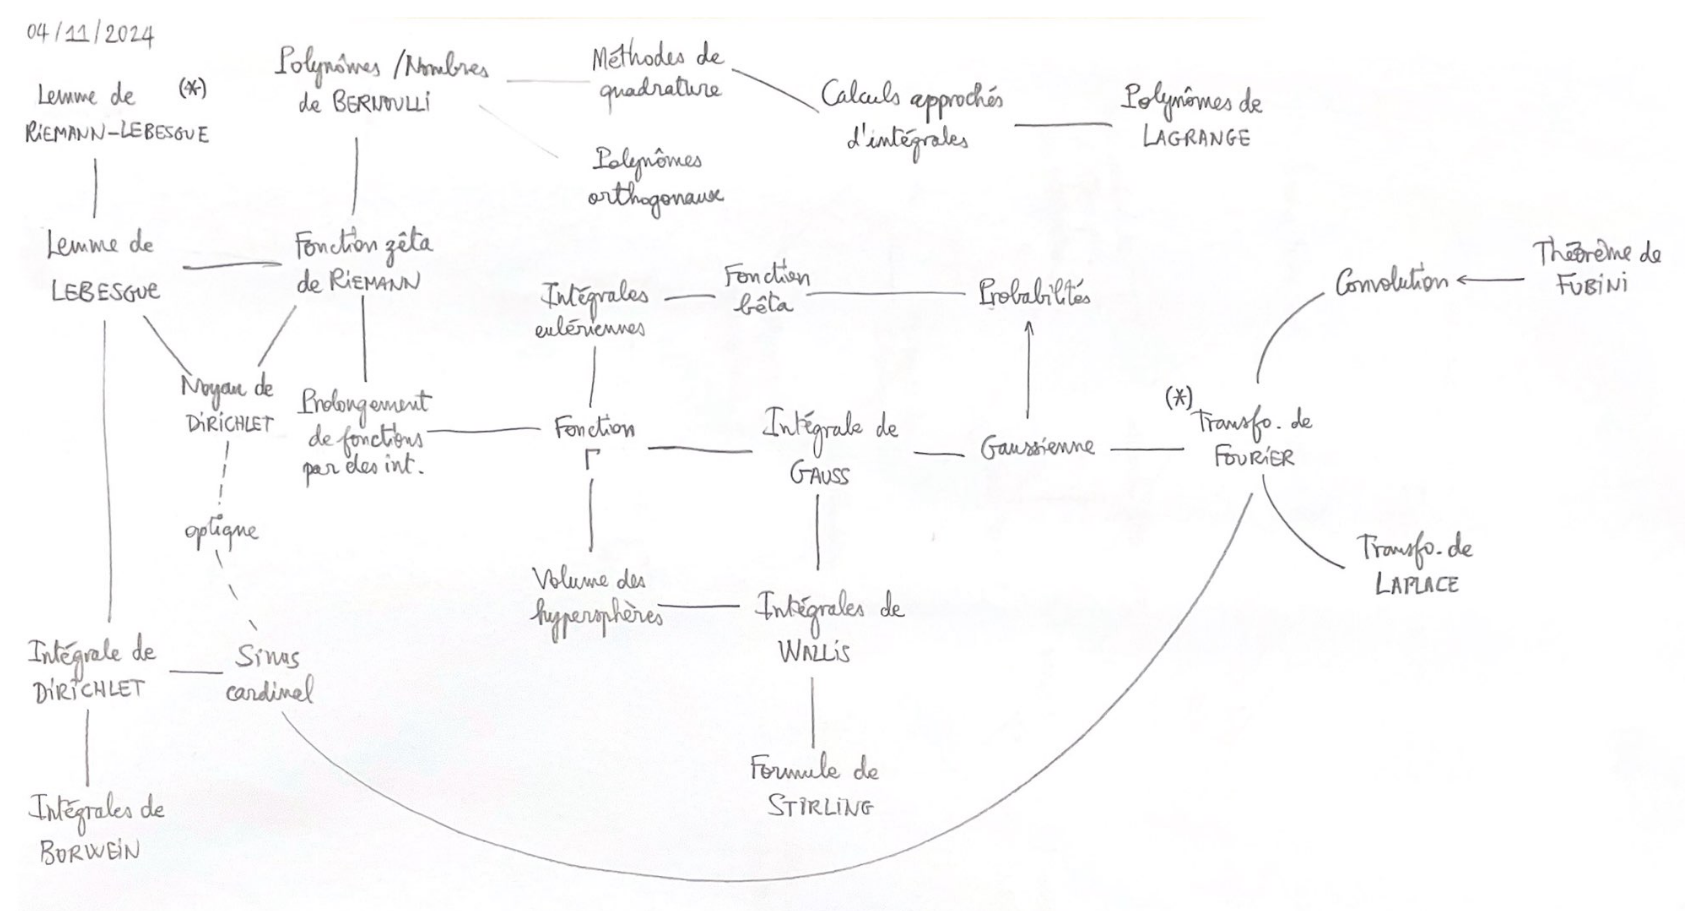
\includegraphics[width=1\linewidth]{chapitres/integration/documents/diagramme_integration.png}
    \caption{Ébauche d'un diagramme des chapitres}
\end{figure}

\todoinline{Chapitres validés : \\
01 : Changement de titre\\
02 : J'ai ajouté un encadré exercice à valider - Le titre de la figure, je le trouve bien - Les liens avec Bernoulli, ça me va mais garder l'encadrer pour rester self-contained.\\
03 : Relire Simpson - Dessins à compléter\\
04 : Peut être un dessin de plus\\
05 : validé \\
07 : Ajouter un graphique ?.\\
08 : Proposition de déplacement\\
09 : TF gaussienne : supprimé car intégré au 10\\
10 : Quelques citations à ajouter\\
11 : Quelques illustrations à terminer\\
12 : Presque validé. Illustrer les boules ?\\
13 : Presque validé après grosse modification pour bêta.\\
14 : Presque validé en supprimant le produit de convolution.\\
}

\todoinline{Créer une annexe avec les théorèmes utilisés ? Comme l'intégration par parties ? Ou alors on met juste un index des théorèmes et il n'y a ensuite qu'à aller chercher dans des livres... ou wikipedia...}

% Régler todo & Mise en forme
\section{Aire et fonction réciproque}

\begin{prop}
Soit $f$ de classe $\mathscr{C}^1$ sur $\interff{a}{b}$ telle que $f'$ soit strictement positive sur $\interff{a}{b}$. Alors,
\[
\int_{a}^{b} f(t) \d t + \int_{f(a)}^{f(b)} f^{-1}(t) \d t = b f(b) - a f(a).
\]
\end{prop}

\begin{elemsolution}
    \begin{enumerate}
    \item Comme $f' > 0$, alors $f$ est strictement croissante. Comme $f$ est continue, d'après le théorème de la bijection monotone, $f$ réalise une bijection de $\interff{a}{b}$ sur $\interff{f(a)}{f(b)}$.
    
    \item On utilise le changement de variable $\fonctionens[\phi]{\interff{a}{b}}{\interff{f(a)}{f(b)}},\, u \mapsto f(u)$. Alors, $\phi$ est de classe $\mathscr{C}^1$ et
    \begin{align*}
    \int_{f(a)}^{f(b)} f^{-1}(t) \d t
    &= \int_a^b f^{-1}\mathopen{}\big(f(u)\big) f'(u) \d u\\
    &= \int_a^b u f'(u) \d u\\
    &= \big[u f(u)\big]_a^b - \int_a^b f(u) \d u,
    \end{align*}
    où on a réalisé une intégration par parties.
    \end{enumerate}

    Finalement,
    \[
    \int_a^b f(t) \d t + \int_{f(a)}^{f(b)} f^{-1}(t) \d t = b f(b) - a f(a).
    \]
\end{elemsolution}

\begin{figure}[H]
    \centering
    \begin{tikzpicture}[line cap=round, >=latex]

\begin{scope}[local bounding box=struct, scale=1]

    \def\u{0.5}
    \def\v{0.2}

    \def\xa{5}
    \def\ya{0.5}
    \def\xb{6.5}
    \def\yb{1.5}
    \def\xc{8}
    \def\yc{4}

    \path (\xa, \ya)    coordinate (A)
        (\xb, \yb)    coordinate (B)
        (\xc, \yc)  coordinate (C)
        (\ya, \xa)    coordinate (A')
        (\yb, \xb)    coordinate (B')
        (\yc, \xc)  coordinate (C');

    \begin{scope}
        \clip (A') ..controls +(0.05*\u, 0.05*\u) and ( $(B') + (-5*\v, -0.5*\u)$ )..
        (B') ..controls +(5*\v, 0.5*\u) and ( $(C') + (-2*\v, -2*\v)$ )..
        (C') |- cycle;
        %\clip (A') ..controls +(0.05*\u, 0.05*\u) and ( $(B') + (-0.5*\v, -0.5*\u)$ )..
        %(B') ..controls +(5*\v, 0.5*\u) and ( $(C') + (-2*\v, -2*\v)$ )..
        %(C') |- cycle;
        \foreach \x in {\ya00, \ya01,...,\yc.000}   
            \draw[blue!15!white, opacity=0.5] (\x,0) -- ++(0,8);
    \end{scope}

    \fill[blue!15!white] (\ya,0) rectangle ++(\yc-\ya,\xa);

    \begin{scope}
        \clip (A) ..controls +(0.05*\u, 0.05*\u) and ( $(B) + (-0.5*\u, -5*\v)$ )..
        (B) ..controls +(0.5*\u, 5*\v) and ( $(C) + (-2*\v, -2*\v)$ )..
            (C) |- cycle;
        \foreach \x in {\xa.000, \xa.001,...,\xc.000}   
            \draw[red!15!white, opacity=0.5] (\x,-\ya) -- ++(0,10);
    \end{scope}

    \draw[thick, blue] 
        (A') ..controls +(0.05*\u, 0.05*\u) and ( $(B') + (-5*\v, -0.5*\u)$ )..
        (B') ..controls +(5*\v, 0.5*\u) and ( $(C') + (-2*\v, -2*\v)$ )..
        (C') node[right] {$\mathcal{C}_f^{-1}$};
        
    \draw[thick, red] 
        (A) ..controls +(0.05*\u, 0.05*\u) and ( $(B) + (-0.5*\u, -5*\v)$ )..
        (B) ..controls +(0.5*\u, 5*\v) and ( $(C) + (-2*\v, -2*\v)$ )..
            (C) node[above] {$\mathcal{C}_f$};


    \fill[red!15!white] (\xa,0) rectangle ++(\xc-\xa,\ya);

    \draw[gray] (-.5, -.5) -- (\xc + 0.5, \xc.5) node[below left] {\contour{white}{\footnotesize$y = x$}};

    \draw[dashed] (\xa, 0) node[black,below]{\footnotesize$a$} -- (A);
    \draw[dashed] (0, \ya) node[black,left]{\footnotesize$f(a)$} -- (A);
    
    \draw[dashed] (\xc, 0) node[black,below]{\footnotesize$b$} -- (C);
    \draw[dashed] (0, \yc) node[black,left]{\footnotesize$f(b)$} -- (C);

    \draw[dashed] (0, \xa) node[black,left]{\footnotesize$a$} -- (A');
    \draw[dashed] (\ya, 0) node[black,below]{\footnotesize$f(a)$} -- (A');
    
    \draw[dashed] (0, \xc) node[black,left]{\footnotesize$b$} -- (C');
    \draw[dashed] (\yc, 0) node[black,below]{\footnotesize$f(b)$} -- (C');

    \draw[->, black] (5.5,2) node[above] 
    {\footnotesize \contour{white}{$\displaystyle \int_a^b f(t)\, \mathrm{d} t$}} to [out=-90,in=180] ($(7,1.5)$);

    % \draw[->, black] (3,-0.5) node[below] 
    % {\footnotesize \contour{white}{$\displaystyle \int_{f(a)}^{f(b)} f^{-1}(t)\, \mathrm{d} t$}} to [out=70,in=-70] ($(3,1.5)$);
    \node at ((2.5, 5) {\footnotesize \contour{blue!15!white}{$\displaystyle \int_{f(a)}^{f(b)} f^{-1}(t)\, \mathrm{d} t$}};

    \draw[thick, ->] (-.5, 0) -- (\xc + 0.5, 0) node[above] {$x$};
    \draw[thick, ->] (0, -.5) -- (0, \xc + 0.5) node[left] {$y$};

\end{scope}

\end{tikzpicture}
    \caption{Illustration géométrique de la formule d'intégration par parties}
    \label{fig:i_01-une_propriete_geometrique_de_l_integrale}
\end{figure}

\begin{comment}
\begin{remarque}
La représentation graphique \ref{fig:i_01-une_propriete_geometrique_de_l_integrale} permet d'illustrer géométriquement la formule d'intégration par parties.

En effet, si $f$, $g$ sont de classe $\mathcal{C}^1$ et strictement monotones, alors elles sont bijectives. On a de plus \mbox{$\big(f \circ g^{-1}\big)^{-1} = g \circ f^{-1}$}. Ainsi, en appliquant la relation précédente à la fonction $f \circ g^{-1}$, on obtient
\begin{align*}
\int_{g(a)}^{g(b)} \big(f \circ g^{-1}\big)(u) \d u + \int_{(f\circ g^{-1})(g(a))}^{(f\circ g^{-1})(g(b))} \big(f \circ g^{-1}\big)^{-1}(u) \d u &= \begin{multlined}[t] 
g(b) \big(f \circ g^{-1}\big)\big(g(b)\big) \\
- g(a) \big(f \circ g^{-1}\big)\big(g(a)\big)
\end{multlined} \\
\int_{g(a)}^{g(b)} \big(f \circ g^{-1}\big)(u) \d u + \int_{f(a)}^{f(b)} \big(g \circ f^{-1}\big)(u) \d u
&= g(b) f(b) - g(a) f(a).
\end{align*}

Ainsi, en effectuant le changement de variable $t \mapsto g(t)$ (resp. $t \mapsto f(t)$) dans la première (resp. seconde) intégrale, on retrouve la formule d'intégration par parties :
\[
\int_a^b f(t) g'(t) \,\mathrm{d}t + \int_a^b g(t) f'(t) \,\mathrm{d}t = f(b) g(b) - f(a) g(a).
\]
\end{remarque}
\end{comment}

% Régler todo & Mise en forme
\section{Lemme de \textsc{Lebesgue}}

\todoinline{Parvenir à décommenter le marginnote suivant. D'après mes recherches sur internet, il faudrait "externaliser" la compilation des figures en pdflatex qui demandent trop de ressources.}

\begin{lemme}
% \marginnote[0cm]{Source : \cite{maths-france} Planche no 37. Intégration sur un segment}
Soit $a < b$.
\begin{enumerate}
\item On suppose que $f$ est une fonction de classe $\mathscr{C}^1$ sur $[a, b]$. Alors,
\[
\lim_{ \lambda \to +\infty} \int_a^b \sin(\lambda t) f(t) \d t = 0.
\]

\item Redémontrer le même résultat en supposant simplement que la fonction $f$ est continue par morceaux sur~$[a, b]$.
\end{enumerate}
\end{lemme}

\todoinline{
Ajout du graphique suivant, à supprimer ou améliorer en coloriant les aires positives et négatives ?
}

\todoarmand{Je suis partant pour laisser le graphique, j'ai ajouté une version avec les aires colorées.}

On constate sur la figure suivante que plus $\lambda$ est grand, plus les oscillations sont élevées et plus les aires comptées positivement et négativement se compensent.
\begin{center}
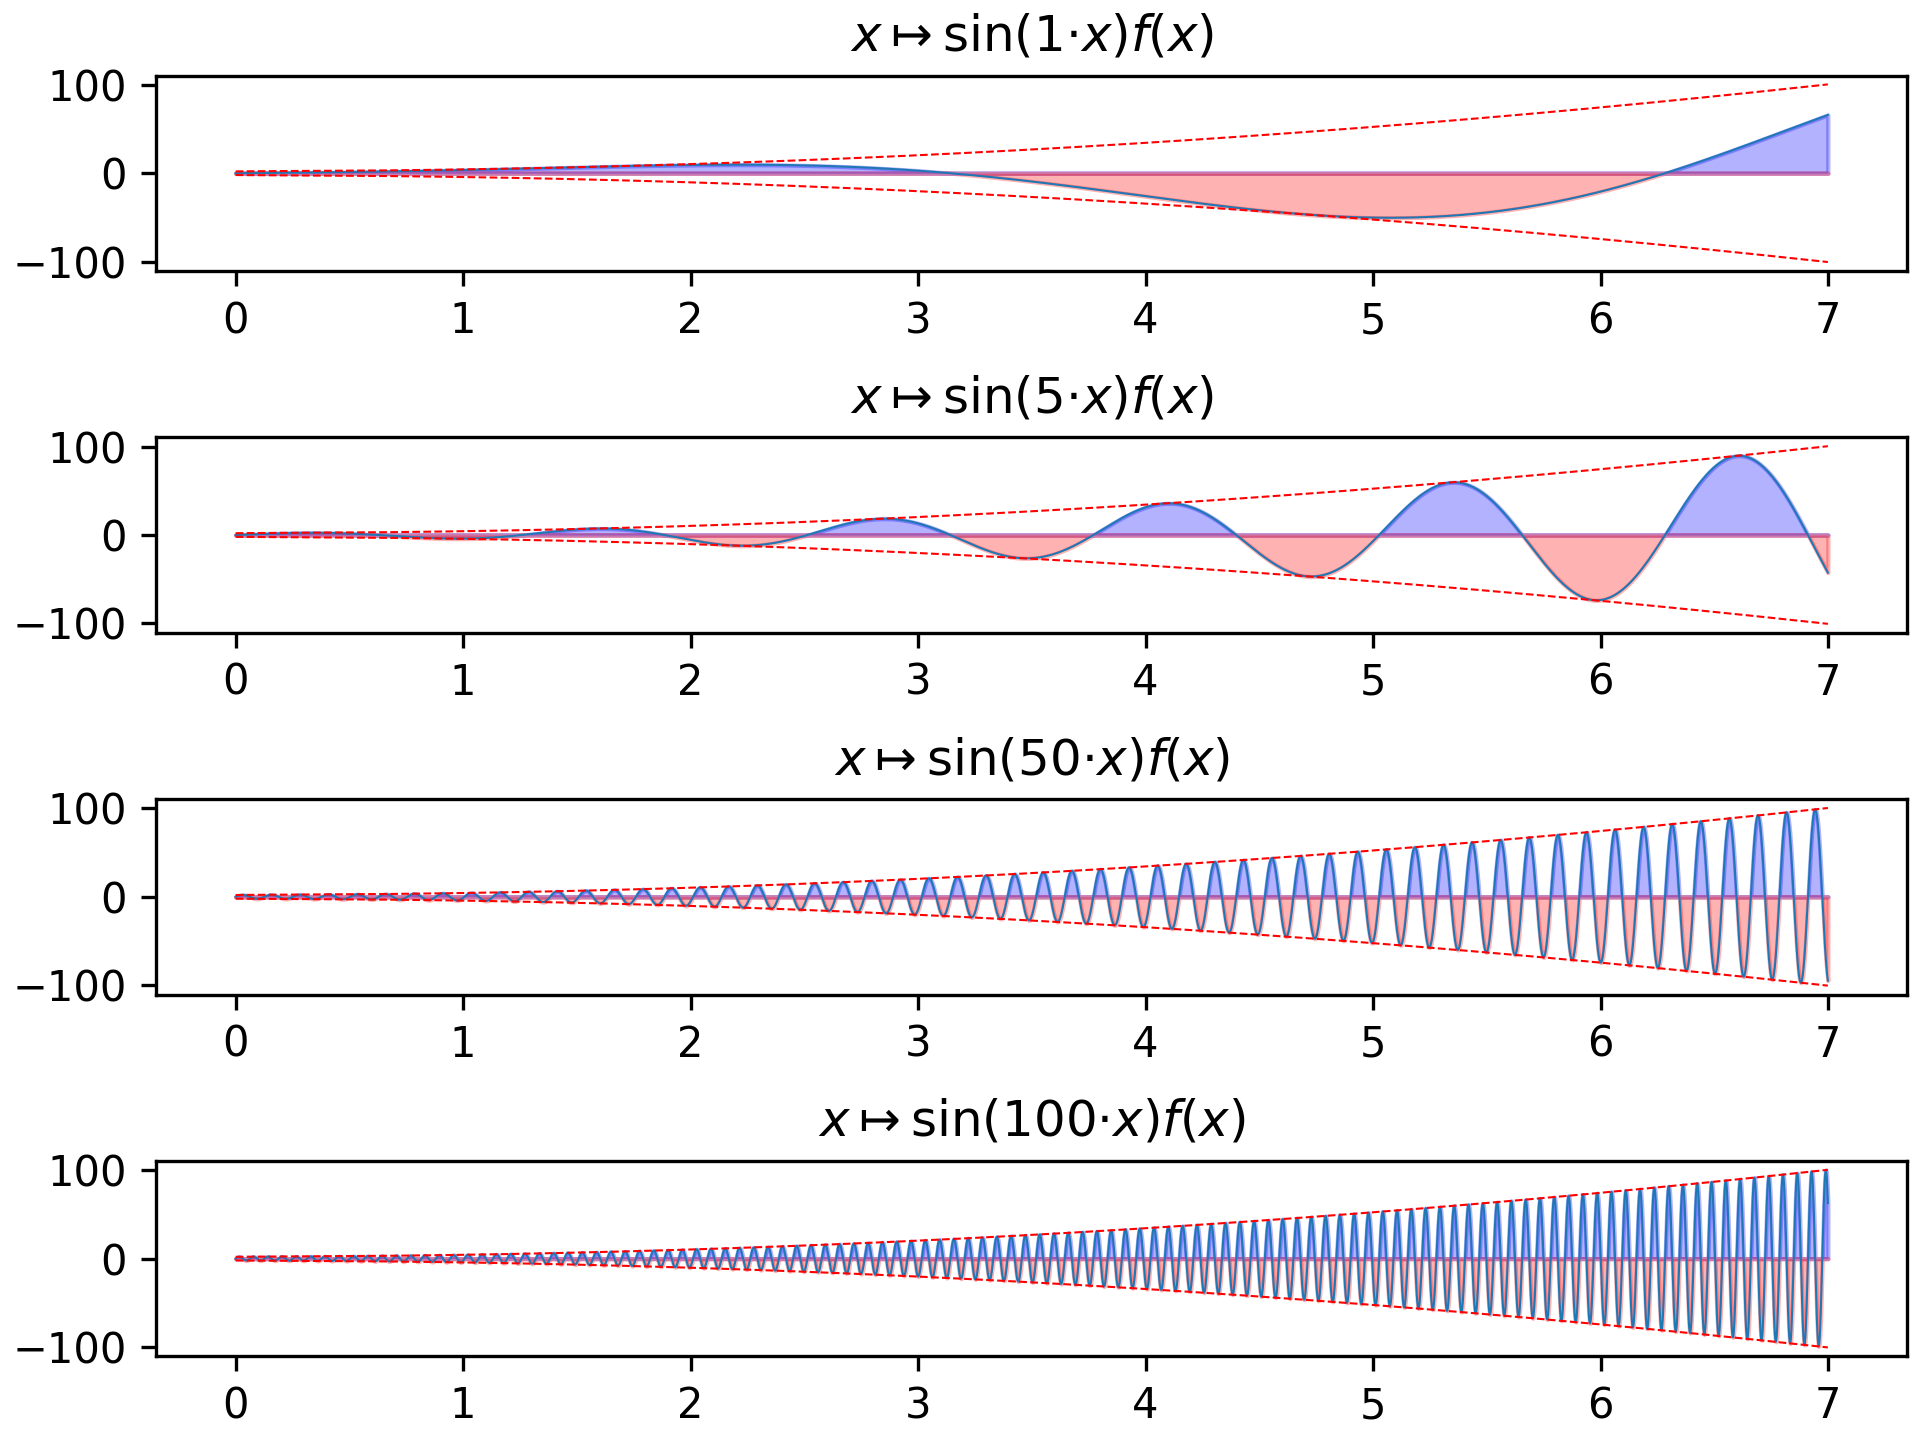
\includegraphics[width=0.75\textwidth]{illustrations/integration-02_lebesgue.png}
\end{center}

\begin{solution}
    \begin{enumerate}
        \item Puisque la fonction $f$ est de classe $\mathscr{C}^1$ sur $[a, b]$, on peut effectuer une intégration par parties qui fournit pour $\lambda > 0$:
        $$\left| \int_a^b f(t) \sin(\lambda t) \d t \right| = \left| \frac{1}{\lambda} \left( -\big[ \cos(\lambda t) f(t) \big]_a^b + \int_a^b f'(t) \cos(\lambda t) \d t  \right) \right| \leqslant \frac{1}{\lambda} \left( |f(a)| + |f(b)| + \int_a^b |f'(t)| \d t \right).$$
        Cette dernière expression tend vers $0$ quand $\lambda$ tend vers $+ \infty$, et donc $\int_a^b f(t) \sin(\lambda t) \d t$ tend vers $0$ quand $\lambda$ tend vers $+\infty$.
        \item Si la fonction $f$ est simplement supposée continue par morceaux, on ne peut donc plus effectuer une intégration par parties. \\
        Le résultat est clair si $f = 1$, car pour $\lambda > 0$, $\left| \int_a^b \sin(\lambda t) \d t \right| = \left| \frac{\cos(\lambda a) - \cos(\lambda b)}{\lambda} \right| \leqslant \frac{2}{\lambda}$. \\
        Le résultat s'étend aux fonctions constantes par linéarité de l'intégrale puis aux fonctions constantes par morceaux par additivité par rapport à l'intervalle d'intégration, c'est-à-dire aux fonctions en escaliers. Pour toute fonction $g$ continue par morceaux sur $[a, b]$, on note $\|g\|_{\infty} = \sup_{[a, b]} |g|$.\\
        Soit alors $f$ une fonction continue par morceaux sur $[a, b]$. \\
        \todoinline{Là on admet un théorème d'approximation non trivial et hors programme en PCSI. Il faut voir ce qu'on indique en introduction du chapitre ?}
        Soit $\varepsilon > 0$. Il existe une fonction en escalier $\varphi$ telle que $\|f - \varphi\|_\infty \leq \varepsilon$. De plus, d'après le point précédent, il existe un réel $\lambda_0$ strictement positif tel que pour tout $\lambda > \lambda_0$,
        \[
        \left|\int_a^b \sin(\lambda t) \varphi(t) \d t\right| \leq \varepsilon.
        \]
        Finalement, d'après l'inégalité triangulaire, pour tout $\lambda > \lambda_0$,
        \begin{align*}
        \left|\int_a^b f(t) \sin(\lambda t) \d t\right|
        &\leq         \left|\int_a^b (f(t) - \varphi(t)) \sin(\lambda t) \d t\right| + \left|\int_a^b \varphi(t) \sin(\lambda t) \d t\right|\\
        &\leq \norme{f - \varphi}_\infty (b - a) + \varepsilon\\
        &\leq \varepsilon (1 + b - a).
        \end{align*}
Finalement, $\lim\limits_{\lambda \to +\infty} \int_a^b f(t) \sin(\lambda t) \d t = 0$.
        \end{enumerate}
\end{solution}


% \todoinline{
% La variante proposée ci-dessous me semble difficile.
%
% Le calcul de $\sum \frac{1}{n^2}$ est classique et pourrait être directement généralisé avec St Cyr 1995 - Je mets une version dans le dossier /chapitres/integration/documents. En plus on ferait un peu de polynômes de Bernoulli.
%
% Le calcul de l'intégrale de Dirichlet est top.
% }

% \todoarmand{Cela me convient, nous pouvons supprimer la variante. On pourrait la remplacer par le  mais en renvoyant vers un exercice du chapitre polynômes.}

\bigskip


\todoinline{Ajouter des liens dans le texte ci-dessous.}

Nous allons utiliser le lemme de Lebesgue pour calculer certaines valeurs de la fonction $\zeta$ de Riemann. Nous verrons ultérieurement une autre utilisation au calcul de la valeur de l'intégrale de Dirichlet.

\todoinline{Partie re-rédigée, à relire !}

\todoinline{Citer sujet St Cyr 1995}

\todoinline{Faire référence à une section sur $\zeta$ et une section sur Bernoulli}

\todoinline{Dans la partie sur Bernoulli, il faudra :
la symétrie, la dérivée et les valeurs de $B_2(0)$ et $B_4(0)$}

On note $(B_n)$ la suite des polynômes de Bernoulli et, pour tout $x > 1$, $\zeta(x) = \sum\limits_{k=1}^{+\infty} \frac{1}{k^x}$.

\begin{theo}
Pour tout $m \geq 1$, $\zeta(2m) = (-1)^{m-1} (2 \pi)^{2m} \frac{B_{2m}(0)}{2}$.
\end{theo}

On rappelle que 
\begin{align*}
B_n(1 - x) &= (-1)^n B_n(x),\\
B_n'(x) &= n B_{n-1}(x).
\end{align*}

\begin{elem_sol}
Pour $k$ et $n$ entiers strictement positifs, on défnit:
\[
I_{n, k} = \int_0^1 B_n(t) \cos(2 k \pi t) \d t.
\]

\begin{enumerate}
\item Pour tout entier $p > 0$,
\[
I_{2p, k} = \frac{(-1)^{p-1}}{(2 k \pi)^{2p}} \quad \text{et} \quad I_{2p+1,k} = 0.
\]

En effet, en utilisant deux intégrations par parties successives,
\[
I_{n,k} = \frac{1}{4k^2 \pi^2} \big(B_{n-1}(1) - B_{n-1}(0) - I_{n-2, k} \big).
\]
De plus, $I_{0,k} = 0$, $I_{1,k} = 0$, $I_{2,k} = \frac{1}{4 \pi^2}$? Donc,
\[
\forall n \geqslant 3,\, I_{n,k} = - \frac{1}{4 k^2 \pi^2}I_{n-2, k}.
\]
On obtient ainsi le résultat annoncé
\end{enumerate}

Pour tout entier naturel $n$ strictement positif, on pose:
\[
\forall t \in \interoo{0}{1}, \quad \varphi_n(t) = \frac{B_n(t) - B_n(0)}{\sin(\pi t)}.
\]

\begin{enumerate}[resume]
\item Pour tout $n \geq 2$, la fonction $\varphi_n$ est prolongeable par continuité à $\interff{0}{1}$ et que le prolongement est de classe $\mathscr{C}^1$. En effet,

\begin{itemize}
\item D'après les quotients de fonctions de classe $\mathscr{C}^1$ dont le dénominateur ne s'annule pas, la fonction $\varphi_n$ est de classe $\mathscr{C}^1$ sur $\interoo{0}{1}$.

\item La fonction $B_n$ étant polynomiale, elle est de classe $\mathscr{C}^1$ en $0$ et, en utilisant la formule de \textsc{Taylor}--\textsc{Young},
\begin{align*}
\varphi_n(t) &= \frac{B'_n(0)t + \frac{B''_n(0)}{2}t^2 + o(t^2)}{\pi t \big(1 + o(t) \big)} \\
&= \frac{B'_n(0)}{\pi} + \frac{B''_n(0)}{2 \pi}t + o(t).
\end{align*}

Ainsi, $\lim\limits_0 \varphi_n = \frac{B'_n(0)}{\pi}$ et $\varphi_n$ est une fonction prolongeable par continuité en $0$.

\item
% De plus, $\lim\limits_{t \to 0} \frac{\varphi_n(t) - \frac{B'_n(0)}{\pi}}{t} = \frac{B''_n(0)}{2 \pi}$.
%
De plus, pour tout $t$ non nul, $\varphi'_n(t) = \frac{B'_n(t) \sin(\pi t) - \big(B_n(t) - B_n(0) \big) \pi \cos(\pi t)}{\sin(\pi t)^2}$. Ainsi, en effectuant un développement limité à l'ordre $2$ du numérateur, alors $\lim\limits_{t \to 0} \varphi'_n(t) = \frac{1}{2 \pi} B''_n(0)$.

D'après le théorème de prolongement des dérivées, $\varphi_n$ est prolongeable en une fonction de classe $\mathscr{C}^1$ sur $\interfo{0}{1}$.

Enfin, $\varphi_n(1-t) = (-1)^n \frac{B_n(t) - B_n(1)}{\sin(\pi t)}$. Comme, pour tout $n \geqslant 2$, $B_n(0) = B_n(1)$, alors la fonction $\varphi_n$ est bien prolongeable en une fonction de classe $\mathscr{C}^1$ sur $\interff{0}{1}$.
\end{itemize}
\end{enumerate}

Pour tout $N$ entier naturel non nul et $t \in \interoo{0}{1}$, on pose :
\[
D_n(t) = 1 + 2 \sum_{k=1}^N \cos(2k \pi t) = \frac{\sin\big((2N+1) \pi t \big)}{\sin(\pi t)}.
\]

\begin{enumerate}[resume]
\item Cette quantité, appelée noyau de Dirichlet, s'exprime simplement à l'aide de la fonction sinus :
\[
D_n(t) = \frac{\sin\big((2N+1) \pi t \big)}{\sin(\pi t)}.
\]
En effet, pour tout $t \in \interoo{0}{1}$, $\e^{2 \i k \pi t} \not= 1$. Ainsi, d'après la somme des termes d'une suite géométrique, 
    \begin{align*}
        \sum_{k=0}^N \e^{2 \i k \pi t} &= \frac{\e^{2 \i (N+1) \pi} - 1}{\e^{2 \i \pi} - 1} \\
        &= \e^{\i N \pi} \frac{\sin(N+1) \pi t}{\sin(\pi t)}. \\
        \sum_{k=0}^N \cos(2 k \pi t) &= \cos(N \pi t) \frac{\sin \big((N+1) \pi t \big)}{\sin(\pi t)}\text{, en prenant les parties réelles,} \\
        1 + 2 \sum_{k=1}^N \cos(2 k \pi t) &= 2 \frac{\cos(N \pi t) \sin \big((N+1) \pi t\big)}{\sin(\pi t)} - 1 \\
        &= \frac{\sin\big((2N+1) \pi t \big) + \sin( \pi t)}{\sin(\pi t)} - 1 \\
        &= \frac{\sin\big((2N+1) \pi t \big)}{\sin(\pi t)}.
    \end{align*}

\item Ainsi,
\[
\int_0^1 \varphi_{2m}(t) \sin \big((2N+1) \pi t \big) \d t
= - B_{2m}(0) + 2 \sum_{k=1}^N \frac{(-1)^{m-1}}{(2 k \pi)^{2m}}.
\]

En effet, d'après la définition de $\varphi_{2m}$,
\begin{align*}
\int_0^1 \varphi_{2m}(t) \sin \big((2N+1) \pi t \big) \d t &= \int_0^1 \big(B_{2m}(t) - B_{2m}(0) \big) \frac{\sin\big((2N+1) \pi t \big)}{\sin(\pi t)} \d t \\
&= \int_0^1 \big( B_{2m}(t) - B_{2m}(0) \big) \d t + \cdots \\
&\cdots + 2 \sum_{k=1}^N \int_0^1 \big(B_{2m}(t) - B_{2m}(0) \big) \cos(2 k \pi t) \d t \\
&= - B_{2m}(0) + 2 \sum_{k=1}^N \frac{(-1)^{m-1}}{(2 k \pi)^{2m}}.
\end{align*}

\item D'après le lemme de Lebesgue,
\[
\lim_{N\to+\infty} \int_0^1 \varphi_{2m}(t) \sin \big((2N+1) \pi t \big) \d t = 0
\]
et on obtient bien le résultat annoncé.
\end{enumerate}
\end{elem_sol}


\begin{remarque}
En utilisant les valeurs remarquables des premiers polynômes de Bernoulli, on obtient
\begin{align*}
\sum_{k=1}^{+\infty} \frac{1}{k^2} &= 2 \pi^2 B_2(0) = \frac{\pi^2}{6} \\
\sum_{k=1}^{+\infty} \frac{1}{k^4} &= -2^3 \pi^4 B_4(0) = \frac{\pi^4}{90}.
\end{align*}
\end{remarque}

% Régler todo & Mise en forme
\section{Calculs approchés d'intégrales}

Nous abordons dans cette section quelques méthodes dont le but est d’estimer la valeur numérique de l'intégrale d'une fonction donnée $f$ définie sur un domaine borné $\interff{a}{b}$:
\[
I = \int_a^b f(t) \d t.
\]
Ces méthodes nous fourniront une valeur approchée $\widetilde{I}$ de l'intégrale $I$ de sorte que \chevron{$\widetilde{I} \approx I$}. \\
Soient $a$ et $b$ deux réels tels que $a < b$. Pour tout entier naturel $p$ non nul, on note $(x_i)_{i\in\llbracket 0, p \rrbracket}$ la subdivision régulière de $[a, b]$ de pas $\frac{b-a}{p}$. Ainsi, pour tout $i \in \llbracket 0, p \rrbracket$,
\[
x_i = a + i\, \frac{b-a}{p}.
\]

\begin{defi}
Une méthode d'intégration est d'\emph{ordre} au moins $n$ si elle est exacte (\emph{i.e.} $\widetilde{I} = I$) pour les polynômes de degrés inférieurs ou égaux $n$ et non exacte pour au moins un polynôme de degré $n+1$.
\end{defi}

%-----------
\subsection{Méthode des rectangles à gauche}

La méthode des rectangles à gauche consiste, pour chacun des intervalles de la subdivision, à approcher l'aire sous la courbe représentative de $f$ par celle d'un rectangle dont la hauteur correspond à la valeur de $f$ sur la borne de gauche. Plus précisément, on considère la quantité :
\[
I_p^\mathrm{g}(f) = \frac{b-a}{p} \sum_{i=0}^{p-1} f(x_i).
\]

\begin{marginfigure}[-3cm]
    \centering
    %https://tex.stackexchange.com/questions/476702/riemann-sum-approaches-area-under-curve

\begin{tikzpicture}[scale=0.8,declare function={f(\x)=((1/3)*(\x)^(3)-3*(\x)^(2)+8*\x-3;}]
\coordinate (start) at (.8,{f(.8)});
\coordinate (x0) at (1,{f(1)});
\coordinate (x1) at (2,{f(2)});
\coordinate (x2) at (3,{f(3)});
\coordinate (x3) at (4,{f(4)});
\coordinate (x4) at (5,{f(5)});
\coordinate (end) at (5.05,{f(5.05)});
\draw[fill=teal!20!white] (1,0) rectangle (2,{f(1)});
\draw[fill=teal!20!white] (2,0) rectangle (3,{f(2)});
\draw[fill=teal!20!white] (3,0) rectangle (4,{f(3)});
\draw[fill=teal!20!white] (4,0) rectangle (5,{f(4)});
%\draw (5,0)--(5,{f(5)});
\draw [-latex] (-0.5,0) -- (6,0) node (xaxis) [below] {$x$};
\draw [-latex] (0,-0.5) -- (0,5) node [left] {$f(x)$};
\foreach \x/\xtext in {1/a=x_0 ,2/x_1, 3/x_2 , 4/x_3 , 5/b=x_4}
 \draw[xshift=\x cm] node[below=2pt,fill=white,font=\small, anchor=south, yshift=-5mm] {$\xtext$};
\draw[domain=.5:5.3,samples=200,variable=\x,blue,thick] plot ({\x},{f(\x)});                 
\foreach \n in {0,1,2,3}
\draw[blue,fill=blue] (x\n) circle (2pt) node[font=\normalsize] {$ $};    
\draw[latex-latex] (2,1)--(3,1) node[midway, anchor=south] {$\frac{b-a}{p}$};      
\end{tikzpicture}
    \caption{Illustration de la méthode des rectangles à gauche}
\end{marginfigure}
\marginnote[3cm]{Animation de la méthode des rectangles à gauche : \url{https://acamanes.github.io/psi/psi_doc/animations/integration_segment/01-methode_des_rectangles_a_gauche.mp4}}

\begin{prop}
La méthode des rectangles à gauche est d'ordre $0$. De plus, si $f$ est de classe $\mathscr{C}^1$, l'erreur commise est en $O(1/p)$.
\end{prop}

\begin{exercice}
Soit $f$ une fonction de classe $\mathscr{C}^1$ sur le segment $\interff{a}{b}$. On note $F$ une primitive de $f$ et $M_1 = \sup_{\interff{a}{b}} \module{f'}$.
\begin{questions}
\item Montrer que
\[
\forall i \in \interent{0}{p-1},\quad 
\module{F(x_{i+1}) - F(x_i) - (x_{i+1} - x_i) F'(x_i)} \leqslant \frac{M_1}{2} (x_{i+1}-x_i)^2.
\]

\item En déduire que
\[
\module{\int_{\interff{a}{b}} f(t) \d t - I_p^\mathrm{g}(f)}
\leqslant \frac{M_1 (b-a)^2}{2 p}.
\]

\item Utiliser la méthode des rectangles à gauche pour calculer une valeur approchée de l'intégrale de la fonction $x \mapsto x - a$.

\item Conclure.
\end{questions}
\end{exercice}

\begin{elemsolution}

\begin{reponses}
\item Il s'agit d'une application de la formule de \textsc{Taylor} avec reste intégal.

\item En utilisant la relation de \textsc{Chasles},
\begin{align*}
\module{\int_{\interff{a}{b}} f(t) \d t - I_p^\mathrm{g}(f)}
&\leqslant \sum_{i=1}^{p-1} \module{\int_{\interff{x_i}{x_{i+1}}} f(x) \d x - (x_{i+1} - x_i) f(x_i)}\\
&\leqslant \sum_{i=1}^{p-1} \frac{M_1}{2} (x_{i+1} - x_i)^2
% &\leq \frac{M_1}{2} (b - a) \sum_{i=1}^{p-1} (x_{i+1} - x_i)\\
\leqslant \frac{M_1 (b-a)^2}{2 p}.
\end{align*}

\item On remarque que, dans ce cas, $M_1 = b - a$ et la borne est atteinte.

\item La méthode des rectangles à gauche est exacte si $f$ est constante. Cependant, le calcul précédent montre que si $\fonctionligne[f]{x}{x - a}$, alors la méthode ne donne pas la valeur exacte de l'intégrale. La méthode est donc d'ordre $0$.
\end{reponses}
\end{elemsolution}

%-----------
\subsection{Méthode des rectangles médians}

La méthode des rectangles médians consiste, pour chacun des intervalles de la subdivision, à approcher l'aire sous la courbe représentative de $f$ par celle d'un rectangle dont la hauteur correspond à la valeur de $f$ au milieu de la subdivision. Plus précisément, on considère la quantité :
\[
I_p^\mathrm{m}(f) = \frac{b-a}{p} \sum_{i=0}^{p-1} f\left(\frac{x_i + x_{i+1}}{2} \right).
\]

\begin{prop}
La méthode des rectangles médians est d'ordre $1$. De plus, si $f$ est de classe $\mathscr{C}^2$, l'erreur commise est en $O(1/p^2)$.
\end{prop}

\begin{marginfigure}[-3cm]
    \centering
    \begin{tikzpicture}[scale=0.8,declare function={f(\x)=((1/3)*(\x)^(3)-3*(\x)^(2)+8*\x-3;}]
\coordinate (start) at (.8,{f(.8)});
\coordinate (x0) at (1.5,{f(1.5)});
\coordinate (x1) at (2.5,{f(2.5)});
\coordinate (x2) at (3.5,{f(3.5)});
\coordinate (x3) at (4.5,{f(4.5)});
\coordinate (x4) at (5.5,{f(5.5)});
\coordinate (end) at (5.05,{f(5.05)});
\draw[fill=teal!20!white] (1,0) rectangle (2,{f(1.5)});
\draw[fill=teal!20!white] (2,0) rectangle (3,{f(2.5)});
\draw[fill=teal!20!white] (3,0) rectangle (4,{f(3.5)});
\draw[fill=teal!20!white] (4,0) rectangle (5,{f(4.5)});

\draw[dashed] (1.5, 0) -- (1.5,{f(1.5)});
\draw[dashed] (2.5, 0) -- (2.5,{f(2.5)});
\draw[dashed] (3.5, 0) -- (3.5,{f(3.5)});
\draw[dashed] (4.5, 0) -- (4.5,{f(4.5)});

\draw [-latex] (-0.5,0) -- (6,0) node (xaxis) [below] {$x$};
\draw [-latex] (0,-0.5) -- (0,5) node [left] {$f(x)$};
\foreach \x/\xtext in {1/a=x_0 ,2/x_1, 3/x_2 , 4/x_3 , 5/b=x_4}
 \draw[xshift=\x cm] node[below=2pt,fill=white,font=\small, anchor=south, yshift=-5mm] {$\xtext$};
\draw[domain=.5:5.3,samples=200,variable=\x,blue,thick] plot ({\x},{f(\x)});                 
\foreach \n in {0,1,2,3}
\draw[blue,fill=blue] (x\n) circle (2pt) node[font=\normalsize] {$ $};    
% \draw[latex-latex] (2,1)--(3,1) node[midway, anchor=south] {$\frac{b-a}{p}$};      
\end{tikzpicture}
    \caption{Illustration de la méthode des rectangles médians}
\end{marginfigure}
\marginnote[3cm]{Animation de la méthode des rectangles médians : \url{https://acamanes.github.io/psi/psi_doc/animations/integration_segment/02-methode_des_rectangles_medians.mp4}}

\begin{exercice}
Soit $f$ une fonction de classe $\mathscr{C}^2$ sur le segment $\interff{a}{b}$. On note $F$ une primitive de $f$ et $M_2 = \sup_{\interff{a}{b}} \module{f''}$. Pour tout entier $i \in \interent{0}{p-1}$, on pose $\gamma_i = \frac{x_i + x_{i+1}}{2}$ le milieu du segment $\interff{x_i}{x_{i+1}}$.
\begin{questions}
\item Montrer que
\[
\forall i \in \interent{0}{p-1},\quad 
(x_{i+1} - x_i) f(\gamma_i) = \int_{x_i}^{x_{i+1}} \left(f(\gamma_i) + (t - \gamma_i) f'(\gamma_i) \right) \d t.
\]    

\item Montrer que
\[
\forall i \in \interent{0}{p-1},\quad 
\module{F(x_{i+1}) - F(x_i) - (x_{i+1} - x_i) F'(\gamma_i)} \leqslant \frac{M_2}{24} (x_{i+1} - x_i)^3.
\]

\item En déduire que
\[
\module{\int_{[a,b]} f(t) \d t- I_p^\mathrm{m}(f)} \leqslant \frac{M_2 (b-a)^3}{24 p^2}.
\]

\item Appliquer l'inégalité précédente à la fonction $x \mapsto (x - a)^2$.

\item Conclure.
\end{questions}
\end{exercice}


\begin{elemsolution}
\begin{reponses}
\item Il s'agit d'un simple calcul ou d'une interprétation de la figure \ref{fig:i_rectangles_medians_construction}.

\item Ainsi, d'après la formule de \textsc{Taylor} avec reste intégral,
\begin{align*}
\module{F(x_{i+1}) - F(x_i) - (x_{i+1} - x_i) F'(\gamma_i)}
&= \module{\int_{x_i}^{x_{i+1}} \left(f(t) - f(\gamma_i) - (t - \gamma_i) f'(\gamma_i)\right) \d t}
\leqslant \frac{M_2}{24} (x_{i+1} - x_i)^3.
\end{align*}

\begin{marginfigure}[0cm]
    \centering
    \begin{tikzpicture}[scale=0.8,declare function={f(\x)=((1/3)*(\x)^(3)-3*(\x)^(2)+8*\x-3;}, declare function={g(\x)=-\x+6;},]
\coordinate (xm) at (3,{f(3)});

\draw[fill=teal!20!white] (2,0) rectangle (4,{f(3)});
\fill[red, opacity=0.2,ultra thick] (2,0) -- (2,{g(2)}) -- (4, {g(4)}) -- (4, 0);

\draw[dashed] (3, 0) -- (3,{f(3)});
\draw[dashed] (2, {f(3)}) -- (2,{g(2)});

\draw [-latex] (-0.5,0) -- (6,0) node (xaxis) [below] {$t$};
\draw [-latex] (0,-0.5) -- (0,5);
% \foreach \x/\xtext in {1/a=x_0 ,2/x_1, 3/x_2 , 4/x_3 , 5/b=x_4}
\draw[xshift=2 cm] node[below=2pt,fill=white,font=\small, anchor=south, yshift=-5mm] {$x_i$};
\draw[xshift=3 cm] node[below=2pt,fill=white,font=\small, anchor=south, yshift=-5mm] {$\gamma_i$};
\draw[xshift=4 cm] node[below=2pt,fill=white,font=\small, anchor=south, yshift=-5mm] {$x_{i+1}$};
\draw[domain=.5:5.3,samples=200,variable=\x,blue,thick] plot ({\x},{f(\x)}) node[right] {$f(t)$};  
\draw[domain=1.5:4.5,samples=200,variable=\x,red,thick] plot ({\x},{g(\x)}) node[right] {$f(\gamma_i) + (t - \gamma_i) f'(\gamma_i)$}; 
% \foreach \n in {0,1,2,3}
\draw[blue,fill=blue] (xm) circle (2pt) node[font=\normalsize] {$ $};    
% \draw[latex-latex] (2,1)--(3,1) node[midway, anchor=south] {$\frac{b-a}{p}$};      
\end{tikzpicture}
    \caption{}
    \label{fig:i_rectangles_medians_construction}
\end{marginfigure}

\item Comme pour la méthode des rectangles à gauche, il s'agit d'une application de la formule de \textsc{Chasles}.

\item On montre que la borne est atteinte pour $f : x \mapsto (x - a)^2$.

\item La méthode des rectangles médians est exacte si $f$ est un polynôme de degré $1$. Cependant, si $f$ est la fonction $x \mapsto (x - a)^2$, le calcul précédent montre que la méthode des rectangles médians ne donne pas la valeur exacte de l'intégrale. La méthode est donc d'ordre $1$.
\end{reponses}
\end{elemsolution}

%-----------
\subsection{Méthode des trapèzes}

La méthode des trapèzes consiste, pour chacun des intervalles de la subdivision, à approcher l'aire sous la courbe représentative de $f$ par celle d'un trapèze. Plus précisément, on considère la quantité :
\[
I_p^\mathrm{t}(f) =  \frac{b-a}{p} \sum_{i=0}^{p-1} \frac{f(x_i) + f(x_{i+1})}{2}.
\]

\begin{marginfigure}[0cm]
    \centering
    \begin{tikzpicture}[scale=0.8,declare function={f(\x)=((1/3)*(\x)^(3)-3*(\x)^(2)+8*\x-3;}]
\coordinate (start) at (.8,{f(.8)});
\coordinate (x0) at (1,{f(1)});
\coordinate (x1) at (2,{f(2)});
\coordinate (x2) at (3,{f(3)});
\coordinate (x3) at (4,{f(4)});
\coordinate (x4) at (5,{f(5)});
\coordinate (end) at (5.05,{f(5.05)});

\draw[fill=teal!20!white] (1,0)--(1,{f(1)})--(2,{f(2)})--(2,0);
\draw[fill=teal!20!white] (2,0)--(2,{f(2)})--(3,{f(3)})--(3,0);
\draw[fill=teal!20!white] (3,0)--(3,{f(3)})--(4,{f(4)})--(4,0);
\draw[fill=teal!20!white] (4,0)--(4,{f(4)})--(5,{f(5)})--(5,0);


%\draw (5,0)--(5,{f(5)});
\draw [-latex] (-0.5,0) -- (6,0) node (xaxis) [below] {$x$};
\draw [-latex] (0,-0.5) -- (0,5) node [left] {$f(x)$};
\foreach \x/\xtext in {1/a=x_0 ,2/x_1, 3/x_2 , 4/x_3 , 5/b=x_4}
 \draw[xshift=\x cm] node[below=2pt,fill=white,font=\small, anchor=south, yshift=-5mm] {$\xtext$};
\draw[domain=.5:5.3,samples=200,variable=\x,blue,thick] plot ({\x},{f(\x)});                 
\foreach \n in {0,1,2,3,4}
\draw[blue,fill=blue] (x\n) circle (2pt) node[font=\normalsize] {$ $};    
% \draw[latex-latex] (2,1)--(3,1) node[midway, anchor=south] {$\frac{b-a}{p}$};      
\end{tikzpicture}
    \caption{Illustration de la méthode des trapèzes}
\end{marginfigure}
\marginnote[6cm]{Animation de la méthode des trapèzes : \url{https://acamanes.github.io/psi/psi_doc/animations/integration_segment/03-methode_des_trapezes.mp4}}

\begin{prop}
La méthode des trapèzes est d'ordre $1$. De plus, si $f$ est de classe $\mathscr{C}^2$, l'erreur commise est en $O(1/p^2)$.
\end{prop}

\begin{exercice}
Soit $f$ une fonction de classe $\mathscr{C}^2$. On note $M_2 = \sup_{[a,b]} \module{f''}$. Pour tout $i \in \interent{0}{p-1}$, on note $\phi_i$ l'approximation affine sur $\interff{x_i}{x_{i+1}}$ de $f$ et $g_i = f - \phi_i$.
\begin{questions}
\item Montrer que
\[
\forall i \in \interent{0}{p-1},\quad 
\int_{x_i}^{x_{i+1}} f''(t)\,(t - x_i) (x_{i+1} - t) \d t = - 2 \int_{x_i}^{x_{i+1}} g_i(t) \d t.
\]

\item Montrer que
\[
\forall i \in \interent{0}{p-1},\quad 
\module{\int_{x_i}^{x_{i+1}} f(t) \d t - I_p^\mathrm{t}(f)}
\leqslant \frac{M_2}{2} \cdot \frac{(b - a)^3}{6}.
\]

\item En déduire que
\[
\module{\int_{[a,b]} f(t) \d t - I_p^\mathrm{t}(f)} \leqslant \frac{M_2 (b-a)^3}{12 p^2}.
\]

\item Appliquer l'égalité précédente à la fonction $x \mapsto (x - a)^2$.

\item Conclure.
\end{questions}
\end{exercice}

\begin{elemsolution}
\begin{reponses}
\item Il suffit d'effectuer deux intégrations par parties successives.

\item D'après la relation précédente, on établit que
\begin{align*}
\module{\int_{x_i}^{x_{i+1}} f(t) \d t - I_p^\mathrm{t}(f)}
&\leqslant \int_{x_i}^{x_{i+1}} \module{f(t) - \phi_i(t)} \d t\\
&\leqslant \frac{M_2}{2} \int_{x_i}^{x_{i+1}} (t - x_i) (x_{i+1} - t) \d t
\leqslant \frac{M_2}{2} \cdot \frac{(b - a)^3}{6}.
\end{align*}

\item Comme pour les méthodes précédentes, on utilise la relation de \textsc{Chasles}.

\item On montre que cette borne est atteinte pour $f : x \mapsto (x - a)^2$.

\item La méthode des trapèzes est exacte si $f$ est un polynôme de degré $1$. Cependant, si $f$ est la fonction $x \mapsto (x - a)^2$, le calcul précédent montre qur la méthode des trapèzes ne donne pas la valeur exacte de l'intégrale. La méthode est donc d'ordre $2$.
\end{reponses}
\end{elemsolution}

\begin{marginfigure}[-1cm]
\begin{subfigure}{.5\textwidth}
    \centering
\begin{tikzpicture}[scale=0.6]

\pgfmathdeclarefunction{f}{1}{%
    \pgfmathparse{((#1 - 3) / 1.5)^2 + 1}%
}
% ,declare function={f(\x)=((\x-3)/1.5)^2+1;}]
\coordinate (start) at (.8,{f(.8)});
\coordinate (x0) at (1,{f(1)});
\coordinate (x1) at (1+4/3,{f(1+4/3)});
\coordinate (x2) at (1+8/3,{f(1+8/3)});
\coordinate (x3) at (1+12/3,{f(1+12/3)});
\coordinate (end) at (5.05,{f(5.05)});

\draw[fill=teal!20!white] (1,0)--(1,{f(1)})--(1+4/3,{f(1+4/3)})--(1+4/3,0);
\draw[fill=teal!20!white] (1+4/3,0)--(1+4/3,{f(1+4/3)})--(1+8/3,{f(1+8/3)})--(1+8/3,0);
\draw[fill=teal!20!white] (1+8/3,0)--(1+8/3,{f(1+8/3)})--(5,{f(5)})--(5,0);

\draw[domain=.5:5.3,samples=200,variable=\x,blue,thick] plot ({\x},{f(\x)});                 

\draw[blue,fill=blue] (x0) circle (2pt);    
\draw[blue,fill=blue] (x1) circle (2pt);    
\draw[blue,fill=blue] (x2) circle (2pt);    
\draw[blue,fill=blue] (x3) circle (2pt);    

\end{tikzpicture}
    \caption{Cas convexe}
\end{subfigure}%
\begin{subfigure}{.5\textwidth}
    \centering
\begin{tikzpicture}[scale=0.6
% ,declare function={f(\x)=-((\x-3)/1.5)^2+3.5;}
]

\pgfmathdeclarefunction{f}{1}{%
    \pgfmathparse{-((#1 - 3) / 1.5)^2 + 3.5}%
}
\coordinate (start) at (.8,{f(.8)});
\coordinate (x0) at (1,{f(1)});
\coordinate (x1) at (1+4/3,{f(1+4/3)});
\coordinate (x2) at (1+8/3,{f(1+8/3)});
\coordinate (x3) at (1+12/3,{f(1+12/3)});
\coordinate (end) at (5.05,{f(5.05)});

\draw[fill=teal!20!white] (1,0)--(1,{f(1)})--(1+4/3,{f(1+4/3)})--(1+4/3,0);
\draw[fill=teal!20!white] (1+4/3,0)--(1+4/3,{f(1+4/3)})--(1+8/3,{f(1+8/3)})--(1+8/3,0);
\draw[fill=teal!20!white] (1+8/3,0)--(1+8/3,{f(1+8/3)})--(5,{f(5)})--(5,0);

\draw[domain=.5:5.3,samples=200,variable=\x,blue,thick] plot ({\x},{f(\x)});                 

\draw[blue,fill=blue] (x0) circle (2pt);    
\draw[blue,fill=blue] (x1) circle (2pt);    
\draw[blue,fill=blue] (x2) circle (2pt);    
\draw[blue,fill=blue] (x3) circle (2pt);  

\end{tikzpicture}
    \caption{Cas concave}
\end{subfigure}
\caption{Illustration de la remarque \ref{remarquemethodetrapezes}}
\end{marginfigure}

\begin{remarque}\label{remarquemethodetrapezes}
Lorsque $f$ est de classe $\mathscr{C}^2$ et convexe (resp. concave), alors $f'' \geqslant 0$ (resp. $\leqslant 0$) et, pour tout $p$ entier naturel, \mbox{$\int_{[a,b]} f \leqslant I_p^\mathrm{t}(f)$} (resp. \mbox{$\int_{[a,b]} f \geqslant I_p^\mathrm{t}(f)$}). On obtient ainsi une valeur approchée par excès (resp. par défaut) de l'intégrale.
\end{remarque}

\subsection{Méthode de \textsc{Simpson}}

La méthode de \textsc{Simpson} consiste, pour chacun des intervalles de la subdivision, à approcher la fonction $f$ par un polynôme de degré inférieur ou égal à $2$. Plus précisément, on considère la quantité :
\[
I_p^\mathrm{s}(f) = \frac{b-a}{6 p} \sum_{i=0}^{p-1} \left[f(x_i)+ 4 f\left(\frac{x_i + x_{i+1}}{2}\right) + f(x_{i+1})\right].
\]

\begin{prop}
Dans la méthode de \textsc{Simpson}, si $f$ est de classe $\mathscr{C}^4$, l'erreur commise est en $O(1/p^4)$.
\end{prop}

\todoinline{Tu aurais le courage de vérifier le calcul suivant ?}

\begin{exercice}
Soit $f$ une fonction de classe $\mathscr{C}^4$ sur le segment $[a, b]$. On pose $M_4 = \sup_{[a,b]} \big\vert f^{(4)} \big\vert$.

Pour tout $i \in \interent{0}{p-1}$, notons $\gamma_i = \frac{x_i + x_{i+1}}{2}$ le milieu de la subdivision et $h_i = \frac{x_{i+1} - x_i}{2}$ la moitié de sa longueur.
\begin{questions}
\item Montrer que pour tout $i \in \interent{0}{p-1}$,
\[
F(x_{i+1}) - F(x_i)
= \begin{multlined}[t] 
2 h_i f(\gamma_i) + \frac{h_i{}^3}{3} f''(\gamma_i) \\
+ \frac{h_i{}^5}{24} \int_0^1 (1 - t)^4 \left[f^{(4)}(\gamma_i + t h_i) + f^{(4)}(\gamma_i - t h_i)\right] \d t.
\end{multlined} 
\]

\item Montrer que pour tout $i \in \interent{0}{p-1}$,
\[
\module{f(x_{i+1}) + f(x_i) - 2 f(\gamma_i) - h_i{}^2 f(\gamma_i)} \leqslant \frac{h_i{}^4 \times 2 M_4}{4!}.
\]

\item En déduire que pour tout $i \in \interent{0}{p-1}$,
\[
\module{\int_{x_i}^{x_{i+1}} f(t) \d t - \frac{h_i}{3} \left[f(x_i) + 4 f(\gamma_i) + f(x_{i+1})\right]}
\leqslant \frac{(x_{i+1} - x_i)^5}{720}.
\]

\item Conclure.
\end{questions}
\end{exercice}

\begin{elemsolution}
\begin{reponses}
\item D'après la formule de \textsc{Taylor} avec reste intégral appliquée à une primitive $F$ de $f$,
\begin{align*}
F(\gamma_i + h_i)
&= \begin{aligned}[t]F(\gamma_i) + h_i f(\gamma_i) + \frac{h_i{}^2}{2} f'(\gamma_i) + \frac{h_i{}^3}{6} f''(\gamma_i) + \frac{h_i{}^4}{24} f'''(\gamma_i) \\ + \frac{h_i{}^5}{24} \int_0^1 (1 - t)^4 f^{(4)}(\gamma_i + t h_i) \d t,\\
\end{aligned} \\
\intertext{et}
F(\gamma_i - h_i)
&= \begin{aligned}[t]F(\gamma_i) - h_i f(\gamma_i) + \frac{h_i{}^2}{2} f'(\gamma_i) - \frac{h_i{}^3}{6} f''(\gamma_i) + \frac{h_i{}^4}{24} f'''(\gamma_i) \\ - \frac{h_i{}^5}{24} \int_0^1 (1 - t)^4 f^{(4)}(\gamma_i - t h_i) \d t.
\end{aligned}
\end{align*}

Comme $\gamma_i - h_i = x_i$ et $\gamma_i + h_i = x_{i+1}$, le résultat s'obtient en soustrayant les deux relations précédentes.


\item On applique la formule de \textsc{Taylor} avec reste intégral à la fonction $f$ sur $[\gamma_i - h_i, \gamma_i]$ et $[\gamma_i, \gamma_i + h_i]$.

\item Finalement,
\begin{align*}
\module{\int_{x_i}^{x_{i+1}} f(t) \d t - \frac{h_i}{3} \left[f(x_i) + 4 f(\gamma_i) + f(x_{i+1})\right]}
&\leqslant \module{\frac{h_i}{3} \left[f(x_i) - 2 f(\gamma_i) + f(x_{i+1}) - h_i{}^2 f''(\gamma_i)\right]} + \frac{h_i{}^5 2 M_4}{5! p^5}\\
&\leqslant h_i{}^5 \left[\frac{2}{3 \times 4!} + \frac{2}{5!}\right]\\
&\leqslant \frac{2 h_i{}^5}{45}
\leqslant \frac{(x_{i+1} - x_i)^5}{720}.
\end{align*}

\item On conclut à l'aide de la relation de \textsc{Chasles} :
\[
\module{\int_a^b f(t) \d t - I_p^\mathrm{s}(f)} \leq \frac{M_4 (b-a)^5}{720 p^4}.
\]
% \[
% \module{I_p^s(f) - \int_a^b f(t) \d t} \leq \frac{M_4 (b-a)^5}{2880 p^4}.
% \]
\end{reponses}
\end{elemsolution}

\begin{figure}[H]
    \centering
    \newcommand*{\parabolaShading}[6]{
\fill [cyan!10, domain=(#1:#5), variable=\x] (#1,0)  -- plot 
    (  {\x},{(#2*(\x-#3)*(\x-#5)/((#1-#3)*(#1-#5)))+
            (#4*(\x-#1)*(\x-#5)/((#3-#1)*(#3-#5)))+
            (#6*(\x-#1)*(\x-#3)/((#5-#1)*(#5-#3)))} )
    -- (#5,0) -- cycle;
}
\newcommand*{\parabolaLines}[6]{
\draw plot [domain=(#1-0.25):(#5+0.25)] %can be adjusted
    (   {\x},{(#2*(\x-#3)*(\x-#5)/((#1-#3)*(#1-#5)))+
            (#4*(\x-#1)*(\x-#5)/((#3-#1)*(#3-#5)))+
            (#6*(\x-#1)*(\x-#3)/((#5-#1)*(#5-#3)))} );
}
\newcommand*{\shadeWithBoundedDomainAndColor}[9]{ %first 6 are points; 7,8 are domain; 9 is color
\fill [#9, domain=(#7:#8), variable=\x] (#7,0)  -- plot 
    (  {\x},{(#2*(\x-#3)*(\x-#5)/((#1-#3)*(#1-#5)))+
            (#4*(\x-#1)*(\x-#5)/((#3-#1)*(#3-#5)))+
            (#6*(\x-#1)*(\x-#3)/((#5-#1)*(#5-#3)))} )
    -- (#8,0) -- cycle;
}

\begin{tikzpicture}
\coordinate (p1) at (0.7,3);
\coordinate (p2) at (1,3.3);
\coordinate (p3) at (2,2.5);
\coordinate (p4) at (3,2.5);
\coordinate (p5) at (4,3.5);
\coordinate (p6) at (5,4.1);
\coordinate (p7) at (6,3.4);
\coordinate (p8) at (7,4.1);
\coordinate (p9) at (8,4.6);
\coordinate (p10) at (9,4);
\coordinate (p11) at (9.5,4.7);

%Shading
\parabolaShading{1}{3.3}{2}{2.5}{3}{2.5}
%\parabolaShading{2}{2.5}{3}{2.5}{4}{3.5}
\parabolaShading{3}{2.5}{4}{3.5}{5}{4.1}
%\parabolaShading{4}{3.5}{5}{4.1}{6}{3.4}
\parabolaShading{5}{4.1}{6}{3.4}{7}{4.1}
%\parabolaShading{6}{3.4}{7}{4.1}{8}{4.6}
\parabolaShading{7}{4.1}{8}{4.6}{9}{4}
\shadeWithBoundedDomainAndColor{5}{4.1}{6}{3.4}{7}{4.1}{5}{6}{cyan!30}

% the curve
\draw[thick,cyan]
  (p1) to[out=70,in=180] (p2) to[out=0,in=150]
  (p3) to[out=-50,in=230] (p4) to[out=30,in=220]
  (p5) to[out=50,in=150] (p6) to[out=-30,in=180]
  (p7) to[out=0,in=230] (p8) to[out=40,in=180]
  (p9) to[out=-30,in=180] (p10) to[out=0,in=260] (p11);

%uncomment the rest for all of the parabolas
\parabolaLines{1}{3.3}{2}{2.5}{3}{2.5}
%\parabolaLines{2}{2.5}{3}{2.5}{4}{3.5}
\parabolaLines{3}{2.5}{4}{3.5}{5}{4.1}
%\parabolaLines{4}{3.5}{5}{4.1}{6}{3.4}
\parabolaLines{5}{4.1}{6}{3.4}{7}{4.1}
%\parabolaLines{6}{3.4}{7}{4.1}{8}{4.6}
\parabolaLines{7}{4.1}{8}{4.6}{9}{4}

% vertical lines and labels
\foreach \n/\texto in {2/{a=x_0},3/{x_1},4/{},5/{},6/{x_{k-1}},7/{x_k},8/{},9/{x_{n-1}},10/{b=x_n}}
{
  \draw (p\n|-0,0) -- (p\n);
  \node[below,text height=1.5ex,text depth=1ex,font=\small] at (p\n|-0,0) {$\texto$};
}
% The axes
\draw[-latex] (-0.5,0) -- (10,0) coordinate (x axis);
\draw[-latex] (0,-0.5) -- (0,6) coordinate (y axis);
% labels for the axes
\node[below] at (x axis) {$x$};
\node[left] at (y axis) {$y$};
% label for the function
\node[above,text=cyan] at (p11) {$y=f(x)$};

\end{tikzpicture}
    \caption{Illustration de la méthode de \textsc{Simpson}}
\end{figure}
\todoarmand{Figure à reprendre, pour l'instant reprise de \url{https://tex.stackexchange.com/questions/429634/parabola-through-three-points-with-tikz}}

\todoinline{Très bonne idée}

%-----------
\subsection{Et ensuite ?}

Nous constatons que pour chacune des méthodes précédentes la stratégie est identique :
\begin{itemize}
\item découper le segment en une subdivision régulière $a = x_0 \leqslant \cdots \leqslant x_n = b$,

\item sur chacun des intervalles de cette subdivision, approcher la fonction par une fonction dont l'intégrale est plus simple.

Sur l'intervalle $[x_i, x_{i+1}]$ : pour la méthode des rectangles, on approche la fonction par une droite horizontale, pour celle des trapèzes, par une droite affine passant par les points $(x_i, f(x_i))$ et $(x_{i+1}, f(x_{i+1}))$.
\end{itemize}

Plus généralement, on peut découper le segment $\interff{x_i}{x_{i+1}}$ en une subdivision régulière $x_i = y_{i,0} \leqslant \ldots \leqslant y_{i,p} \leqslant x_{i+1}$. On peut ensuite approcher la fonction par le polynôme d'interpolation de \textsc{Lagrange} qui passe par les points de coordonnées $(y_{i,0}, f(y_{i,0})), \ldots, (y_{i,p}, f(y_{i,p}))$.

Cette méthode est appelée \emph{méthode de \textsc{Newton}--\textsc{Cotes}}.

Plus précisément, on considère une subdivision $0 = y_0 \leqslant \cdots \leqslant y_p = 1$ de l'intervalle $\interff{0}{1}$ et on note $(L_0,\ldots,L_p)$ la famille des \hyperref[sec:polynomes_de_lagrange]{polynômes d'interpolation de \textsc{Lagrange}} associée à cette subdivision, i.e.
\[
\forall i \in \interent{0}{p},\quad L_i(X) = \prod_{j \neq i} \frac{X - y_j}{y_i - y_j}.
\]

On pose alors $\gamma_j = \int_0^1 L_j(t) \d t$.

On approche alors l'intégrale de $f$ sur $[x_i, x_{i+1}]$ par la somme
\[
I_p^i(f) = (x_{i+1} - x_i) \sum_{j=0}^p \gamma_j g(x_i + (x_{i+1} - x_i) y_j),
\]
puis l'intégrale sur le segment $\interff{a}{b}$ par
\[
I_p(f) = \sum_{i=0}^{n-1} (x_{i+1} - x_i) \bigg[ \sum_{j=0}^p \gamma_j f(x_i + (x_{i+1} - x_i) y_j) \bigg].
\] 

On peut montrer que :
\begin{itemize}
\item lorsque $n = 1$, on retrouve la formule des trapèzes.

\item lorque $n = 2$, on retrouve la méthode de \textsc{Simpson}.
\end{itemize}

On peut montrer que la méthode de \textsc{Simpson} est d'ordre $3$. On peut augmenter le nombre des n\oe{}uds où est évaluée la fonction à intégrer ($2$ n\oe{}uds pour la méthode des trapèzes, $3$ pour la méthode de \textsc{Simpson},\ldots). Cependant, lorsque le nombre de n\oe{}uds dépasse $8$, des coefficients négatifs apparaissent ce qui engendre des erreurs d'arrondis. \\

\begin{table}[]
    \centering
    \begin{tblr}{
    hlines,vlines,
    hline{2} = {2pt},
    cells={c}
    }
    \textbf{Méthode} & \textbf{Ordre} & \textbf{Vitesse de conv.} & \textbf{\textsc{Newton}--\textsc{Cotes}} \\
    À gauche & $0$ & $O(1/p)$ & X\\
    À droite & $0$ & $O(1/p)$ & X\\
    Médians & $1$ & $O(1/p^2)$ & X\\
    Trapèzes & $1$ & $O(1/p^2)$ & 1\\
    \textsc{Simpson} & $3$ & $O(1/p^4)$ & 2
    \end{tblr}
    \caption{Résumé des propriétés des méthodes de calculs approchés d’intégrales}
\end{table} % margintable

\todoinline{
Je veux bien que tu t'occupes de ces deux points rapides, je ne maîtrise pas encore les différentes fonctions.

Mettre ici un lien vers un thème sur les polynômes d'interpolation de Lagrange.

On pourrait ajouter vers le livre Demailly - Analyse numérique et équations différentielles}


% Régler todo & Mise en forme
\section{Fonctions décroissantes}

\todoarmand{Pour une raison que je ne comprends pas, je n'arrive plus à compiler deux des figures.}

\todoinline{Ici, on n'a pas de théorème, que des exercices. Ce n'est pas un problème mais chercherait-on une présentation uniforme sur ces premiers thèmes ?}

\begin{exercice}
    \marginnote[0cm]{Source : \cite{exos_oraux} p. 268}
    Soit $\fonctionens[f]{\Rp}{\R}$ une fonction continue, décroissante et intégrable. Montrer que $x f(x) \to 0$ lorsque $x \to +\infty$.
\end{exercice}

\begin{marginfigure}[-2cm]
    \centering
    % \begin{tikzpicture}[scale=0.5]
  
  \def\xmax{4.5}
  \def\ymax{1.5}
  \def\ymin{-2}
  \def\xzero{2}
  \def\x{5}

    \begin{axis}[
        restrict x to domain=0:8,
        samples=100, % you don't need 1000, it only slows things down
        ticks=none,
        xmin = -1, xmax = \xmax+1,
        ymin = \ymin, ymax = \ymax,
        unbounded coords=jump,
        axis x line=middle,
        axis y line=middle,
        % xlabel={$x$},
        % ylabel={$y$},
        x label style={
          at={(axis cs:5.1,0.2)},
          anchor=west,
        },
        every axis y label/.style={
          at={(axis cs:0,1.5)},
          anchor=south
        },
        legend style={
          at={(axis cs:-5.2,4)},
          anchor=west, font=\scriptsize
        },
        declare function={f(\x)=2*e^(-\x^2/2)-(\x/7)^2-1;},
        ] 
      \addplot[name path=A,very thick,color=blue, mark=none, domain=0:\xmax] {f(x)}
          node [above=8mm,near start] {$f\textcolor{black}{(x)}$};
          
      \addplot[mark=*,fill=white] coordinates {(\xzero,{f(\xzero)})};
      \draw[dashed] (axis cs:0,{f(\xzero)}) node[left=1mm] (l) {$f(x_0)$} -| (axis cs:2,0) node[above] (a) {$x_0$}; 
      \draw (axis cs:\x-0.5,0) node[above] {$x$};

    \path [name path=B] (0,0)--(\xmax, 0);
    \addplot [blue!20!white] fill between [of=A and B, soft clip={domain=\xzero:\x}];

    \fill[red!30!white, pattern=north east lines] (\xzero,0) rectangle (\x-0.5,f(\xzero);
    
    \end{axis}

    \draw[->, black, thick] (5, 4) node[above] {$f(x_0) (x - x_0)$} to [out=-90,in=90] ($(4.5,2.6)$);

    \draw[->, black, thick] (4, 1) node[left] {\color{blue}$\displaystyle \int_{x_0}^x f(t)\, \mathrm{d} t$} to [out=0,in=-90] ($(4.5,1.6)$);
    
  \end{tikzpicture}
    \caption{ébauche}
\end{marginfigure}

\begin{elemsolution}
\begin{itemize}
\item Comme $f$ est décroissante, d'après le théorème de la limite monotone, il existe $\ell \in \R \cup \ens{-\infty}$ tel que $\lim\limits_{x\to+\infty} f(x) = \ell$.

\item Montrons par l'absurde que $f$ est positive. S'il existe $x_0 \geqslant 0$ tel que $f(x_0) < 0$, comme $f$ est décroissante,
\[
\forall\ x \geqslant x_0,\quad f(x) \leq f(x_0).
\]
Ainsi,
\[
\forall\ x \geqslant x_0,\quad \displaystyle\int_{x_0}^x f(t) \d t \leqslant f(x_0) (x - x_0).
\]
D'après le théorème d'encadrement, $\lim\limits_{x\to+\infty} \displaystyle\int_{x_0}^x f(t) \d t = -\infty$, ce qui est impossible car $f$ est intégrable. Ainsi, $f$ est à valeurs positives et $\ell \geqslant 0$.

\item Supposons par l'absurde que $\ell > 0$. Alors, il existe un réel $A$ tel que
\[
\forall\ x \geqslant A,\quad f(x) \geqslant \frac{\ell}{2}.
\]
Ainsi,
\[
\forall\ x \geqslant A,\quad \displaystyle\int_A^x f(t) \d t \geqslant \frac{\ell}{2} (x - A).
\]
D'après le théorème d'encadrement, $\lim\limits_{x\to+\infty} \displaystyle\int_A^x f(t) \mathrm{d}t = +\infty$, ce qui est impossible car $f$ est intégrable.

Finalement, $\lim\limits_{x\to+\infty} f(x) = 0$.

\item Soit $x \geqslant 0$. Comme $f$ est décroissante,
\[
\int_x^{2 x} f(t) \d t \leqslant (2 x - x) f(x).
\]

De même,
\[
\int_{x/2}^x f(t) \d t \geqslant \frac{x}{2} f(x).
\]

\begin{marginfigure}
    \centering
    % \begin{tikzpicture}

  % https://copyprogramming.com/howto/how-do-i-draw-arrows-at-coordinate-on-a-plot
  
  \def\xmax{5.5}
  \def\ymax{1.2}
  \def\ymin{-0.2}
  \def\x{2.5}
  \def\xzero{\x/2}

  \def\colfonc{green!70!black}

    \begin{axis}[
        restrict x to domain=0:10,
        samples=100, % you don't need 1000, it only slows things down
        ticks=none,
        xmin = -1, xmax = \xmax+1,
        ymin = \ymin, ymax = \ymax,
        unbounded coords=jump,
        axis x line=middle,
        axis y line=middle,
        axis line style={-latex},
        % xlabel={$x$},
        % ylabel={$y$},
        x label style={
          at={(axis cs:5.1,0.2)},
          anchor=west,
        },
        every axis y label/.style={
          at={(axis cs:0,1.5)},
          anchor=south
        },
        legend style={
          at={(axis cs:-5.2,4)},
          anchor=west, font=\scriptsize
        },
        % ,declare function={f(\x)=e^(-\x^2/8);},
        ] 

\pgfmathdeclarefunction{f}{1}{%
\pgfmathparse{e^(-#1^2/8)}%
}
      \addplot[name path=A,very thick,color=\colfonc, mark=none, domain=0:\xmax] {f(x)} node [above=2mm,near start] {$f$};
          
      % \addplot[mark=*,fill=white] coordinates {(\xzero,{f(\xzero)})};
      % \draw[dashed] (axis cs:0,{f(\xzero)}) node[left=1mm] (l) {$f(x_0)$} -| (axis cs:2,0) node[above] (a) {$x_0$}; 
      \draw (\xzero,0) node[below] {$x/2$};

      \draw[dashed] (axis cs:0,{f(\x)}) node[left=1mm] (l) {$f(x)$} -| (axis cs:\x,0) node[below] (a) {$\vphantom{x/2}x$};
      
      % \draw (\x,0) node[below] {$x$};
      \draw (2*\x,0) node[below] {$\vphantom{x/2}2x$};

    \path [name path=B] (0,0)--(\xmax, 0);
    \addplot [blue!20!white] fill between [of=A and B, soft clip={domain=\xzero:\x}];

    \addplot [red!20!white] fill between [of=A and B, soft clip={domain=\x:2*\x}];

    \fill[pattern color=blue, pattern=north east lines] (\xzero,0) rectangle (\x,f(\x);
    \fill[pattern color=red, pattern=north east lines] (\x,0) rectangle (2*\x,f(\x);

    \end{axis}

    % \draw[->, black, thick] (5, 4) node[above] {$f(x_0) (x - x_0)$} to [out=-90,in=90] ($(4.5,2.6)$);

    % \draw[->, black, thick] (4, 1) node[left] {\color{blue}$\displaystyle \int_{x_0}^x f(t)\, \mathrm{d} t$} to [out=0,in=-90] ($(4.5,1.6)$);
    
\end{tikzpicture}
    \caption{ébauche}
\end{marginfigure}

\todoinline{On pourrait illustrer les deux inégalités précédentes en dessinant les aires sous des rectangles en hachuré et les aires sous les courbes en couleur pastel. On pourrait mettre une couleur pour $[x/2, x]$ et une différente sur $[x, 2x]$}


Ainsi,
\[
\int_x^{2 x} f(t) \d t \leqslant x f(x) \leqslant 2 \int_{x/2}^x f(t) \d t.
\]
En notant $\fonctionligne[F]{x}{\displaystyle\int_0^x f(t) \d t}$, comme $f$ est intégrable, alors $F$ possède une limite finie en $+\infty$.

Ainsi,
\[
F(2 x) - F(x) \leqslant x f(x) \leqslant 2 (F(x) - F(x/2)).
\]

Ainsi, d'après le théorème d'encadrement, $\lim\limits_{x\to 0} x f(x) = 0$.
\end{itemize}
\end{elemsolution}

\todoarmand{Mettre un lien vers \url{http://ddmaths.free.fr/section115.html} ou pas car c'est très classique}



\begin{exercice}
    \marginnote[0cm]{Source : \cite{truc2019} p. 268}
    Soit $\fonctionligne[f]{\interof{0}{1}}{\R}$ une fonction continue, décroissante et intégrable. Alors,
    \[
    \lim\limits_{n \to +\infty} \frac{1}{n} \sum\limits_{k=1}^n f\mathopen{}\left(\frac{k}{n}\right) =\int_0^1 f(t) \d t.
    \]
\end{exercice}

\begin{marginfigure}
    \centering
    %% Creator: Matplotlib, PGF backend
%%
%% To include the figure in your LaTeX document, write
%%   \input{<filename>.pgf}
%%
%% Make sure the required packages are loaded in your preamble
%%   \usepackage{pgf}
%%
%% Also ensure that all the required font packages are loaded; for instance,
%% the lmodern package is sometimes necessary when using math font.
%%   \usepackage{lmodern}
%%
%% Figures using additional raster images can only be included by \input if
%% they are in the same directory as the main LaTeX file. For loading figures
%% from other directories you can use the `import` package
%%   \usepackage{import}
%%
%% and then include the figures with
%%   \import{<path to file>}{<filename>.pgf}
%%
%% Matplotlib used the following preamble
%%   
%%   \usepackage{fontspec}
%%   \setmainfont{DejaVuSerif.ttf}[Path=\detokenize{/home/wayoff/.pyenv/versions/3.8.10/lib/python3.8/site-packages/matplotlib/mpl-data/fonts/ttf/}]
%%   \setsansfont{DejaVuSans.ttf}[Path=\detokenize{/home/wayoff/.pyenv/versions/3.8.10/lib/python3.8/site-packages/matplotlib/mpl-data/fonts/ttf/}]
%%   \setmonofont{DejaVuSansMono.ttf}[Path=\detokenize{/home/wayoff/.pyenv/versions/3.8.10/lib/python3.8/site-packages/matplotlib/mpl-data/fonts/ttf/}]
%%   \makeatletter\@ifpackageloaded{underscore}{}{\usepackage[strings]{underscore}}\makeatother
%%
\begingroup%
\makeatletter%
\begin{pgfpicture}%
\pgfpathrectangle{\pgfpointorigin}{\pgfqpoint{3.000000in}{3.000000in}}%
\pgfusepath{use as bounding box, clip}%
\begin{pgfscope}%
\pgfsetbuttcap%
\pgfsetmiterjoin%
\definecolor{currentfill}{rgb}{1.000000,1.000000,1.000000}%
\pgfsetfillcolor{currentfill}%
\pgfsetlinewidth{0.000000pt}%
\definecolor{currentstroke}{rgb}{1.000000,1.000000,1.000000}%
\pgfsetstrokecolor{currentstroke}%
\pgfsetdash{}{0pt}%
\pgfpathmoveto{\pgfqpoint{0.000000in}{0.000000in}}%
\pgfpathlineto{\pgfqpoint{3.000000in}{0.000000in}}%
\pgfpathlineto{\pgfqpoint{3.000000in}{3.000000in}}%
\pgfpathlineto{\pgfqpoint{0.000000in}{3.000000in}}%
\pgfpathlineto{\pgfqpoint{0.000000in}{0.000000in}}%
\pgfpathclose%
\pgfusepath{fill}%
\end{pgfscope}%
\begin{pgfscope}%
\pgfsetbuttcap%
\pgfsetmiterjoin%
\definecolor{currentfill}{rgb}{1.000000,1.000000,1.000000}%
\pgfsetfillcolor{currentfill}%
\pgfsetlinewidth{0.000000pt}%
\definecolor{currentstroke}{rgb}{0.000000,0.000000,0.000000}%
\pgfsetstrokecolor{currentstroke}%
\pgfsetstrokeopacity{0.000000}%
\pgfsetdash{}{0pt}%
\pgfpathmoveto{\pgfqpoint{0.580556in}{0.576079in}}%
\pgfpathlineto{\pgfqpoint{2.850000in}{0.576079in}}%
\pgfpathlineto{\pgfqpoint{2.850000in}{2.850000in}}%
\pgfpathlineto{\pgfqpoint{0.580556in}{2.850000in}}%
\pgfpathlineto{\pgfqpoint{0.580556in}{0.576079in}}%
\pgfpathclose%
\pgfusepath{fill}%
\end{pgfscope}%
\begin{pgfscope}%
\pgfpathrectangle{\pgfqpoint{0.580556in}{0.576079in}}{\pgfqpoint{2.269444in}{2.273921in}}%
\pgfusepath{clip}%
\pgfsetbuttcap%
\pgfsetmiterjoin%
\definecolor{currentfill}{rgb}{0.000000,0.501961,0.501961}%
\pgfsetfillcolor{currentfill}%
\pgfsetfillopacity{0.500000}%
\pgfsetlinewidth{1.003750pt}%
\definecolor{currentstroke}{rgb}{0.000000,0.000000,0.000000}%
\pgfsetstrokecolor{currentstroke}%
\pgfsetstrokeopacity{0.500000}%
\pgfsetdash{}{0pt}%
\pgfpathmoveto{\pgfqpoint{0.683713in}{0.576079in}}%
\pgfpathlineto{\pgfqpoint{0.890026in}{0.576079in}}%
\pgfpathlineto{\pgfqpoint{0.890026in}{2.741718in}}%
\pgfpathlineto{\pgfqpoint{0.683713in}{2.741718in}}%
\pgfpathlineto{\pgfqpoint{0.683713in}{0.576079in}}%
\pgfpathclose%
\pgfusepath{stroke,fill}%
\end{pgfscope}%
\begin{pgfscope}%
\pgfpathrectangle{\pgfqpoint{0.580556in}{0.576079in}}{\pgfqpoint{2.269444in}{2.273921in}}%
\pgfusepath{clip}%
\pgfsetbuttcap%
\pgfsetmiterjoin%
\definecolor{currentfill}{rgb}{0.000000,0.501961,0.501961}%
\pgfsetfillcolor{currentfill}%
\pgfsetfillopacity{0.500000}%
\pgfsetlinewidth{1.003750pt}%
\definecolor{currentstroke}{rgb}{0.000000,0.000000,0.000000}%
\pgfsetstrokecolor{currentstroke}%
\pgfsetstrokeopacity{0.500000}%
\pgfsetdash{}{0pt}%
\pgfpathmoveto{\pgfqpoint{0.890026in}{0.576079in}}%
\pgfpathlineto{\pgfqpoint{1.096339in}{0.576079in}}%
\pgfpathlineto{\pgfqpoint{1.096339in}{1.232032in}}%
\pgfpathlineto{\pgfqpoint{0.890026in}{1.232032in}}%
\pgfpathlineto{\pgfqpoint{0.890026in}{0.576079in}}%
\pgfpathclose%
\pgfusepath{stroke,fill}%
\end{pgfscope}%
\begin{pgfscope}%
\pgfpathrectangle{\pgfqpoint{0.580556in}{0.576079in}}{\pgfqpoint{2.269444in}{2.273921in}}%
\pgfusepath{clip}%
\pgfsetbuttcap%
\pgfsetmiterjoin%
\definecolor{currentfill}{rgb}{0.000000,0.501961,0.501961}%
\pgfsetfillcolor{currentfill}%
\pgfsetfillopacity{0.500000}%
\pgfsetlinewidth{1.003750pt}%
\definecolor{currentstroke}{rgb}{0.000000,0.000000,0.000000}%
\pgfsetstrokecolor{currentstroke}%
\pgfsetstrokeopacity{0.500000}%
\pgfsetdash{}{0pt}%
\pgfpathmoveto{\pgfqpoint{1.096339in}{0.576079in}}%
\pgfpathlineto{\pgfqpoint{1.302652in}{0.576079in}}%
\pgfpathlineto{\pgfqpoint{1.302652in}{1.050927in}}%
\pgfpathlineto{\pgfqpoint{1.096339in}{1.050927in}}%
\pgfpathlineto{\pgfqpoint{1.096339in}{0.576079in}}%
\pgfpathclose%
\pgfusepath{stroke,fill}%
\end{pgfscope}%
\begin{pgfscope}%
\pgfpathrectangle{\pgfqpoint{0.580556in}{0.576079in}}{\pgfqpoint{2.269444in}{2.273921in}}%
\pgfusepath{clip}%
\pgfsetbuttcap%
\pgfsetmiterjoin%
\definecolor{currentfill}{rgb}{0.000000,0.501961,0.501961}%
\pgfsetfillcolor{currentfill}%
\pgfsetfillopacity{0.500000}%
\pgfsetlinewidth{1.003750pt}%
\definecolor{currentstroke}{rgb}{0.000000,0.000000,0.000000}%
\pgfsetstrokecolor{currentstroke}%
\pgfsetstrokeopacity{0.500000}%
\pgfsetdash{}{0pt}%
\pgfpathmoveto{\pgfqpoint{1.302652in}{0.576079in}}%
\pgfpathlineto{\pgfqpoint{1.508965in}{0.576079in}}%
\pgfpathlineto{\pgfqpoint{1.508965in}{0.966935in}}%
\pgfpathlineto{\pgfqpoint{1.302652in}{0.966935in}}%
\pgfpathlineto{\pgfqpoint{1.302652in}{0.576079in}}%
\pgfpathclose%
\pgfusepath{stroke,fill}%
\end{pgfscope}%
\begin{pgfscope}%
\pgfpathrectangle{\pgfqpoint{0.580556in}{0.576079in}}{\pgfqpoint{2.269444in}{2.273921in}}%
\pgfusepath{clip}%
\pgfsetbuttcap%
\pgfsetmiterjoin%
\definecolor{currentfill}{rgb}{0.000000,0.501961,0.501961}%
\pgfsetfillcolor{currentfill}%
\pgfsetfillopacity{0.500000}%
\pgfsetlinewidth{1.003750pt}%
\definecolor{currentstroke}{rgb}{0.000000,0.000000,0.000000}%
\pgfsetstrokecolor{currentstroke}%
\pgfsetstrokeopacity{0.500000}%
\pgfsetdash{}{0pt}%
\pgfpathmoveto{\pgfqpoint{1.508965in}{0.576079in}}%
\pgfpathlineto{\pgfqpoint{1.715278in}{0.576079in}}%
\pgfpathlineto{\pgfqpoint{1.715278in}{0.915957in}}%
\pgfpathlineto{\pgfqpoint{1.508965in}{0.915957in}}%
\pgfpathlineto{\pgfqpoint{1.508965in}{0.576079in}}%
\pgfpathclose%
\pgfusepath{stroke,fill}%
\end{pgfscope}%
\begin{pgfscope}%
\pgfpathrectangle{\pgfqpoint{0.580556in}{0.576079in}}{\pgfqpoint{2.269444in}{2.273921in}}%
\pgfusepath{clip}%
\pgfsetbuttcap%
\pgfsetmiterjoin%
\definecolor{currentfill}{rgb}{0.000000,0.501961,0.501961}%
\pgfsetfillcolor{currentfill}%
\pgfsetfillopacity{0.500000}%
\pgfsetlinewidth{1.003750pt}%
\definecolor{currentstroke}{rgb}{0.000000,0.000000,0.000000}%
\pgfsetstrokecolor{currentstroke}%
\pgfsetstrokeopacity{0.500000}%
\pgfsetdash{}{0pt}%
\pgfpathmoveto{\pgfqpoint{1.715278in}{0.576079in}}%
\pgfpathlineto{\pgfqpoint{1.921591in}{0.576079in}}%
\pgfpathlineto{\pgfqpoint{1.921591in}{0.880827in}}%
\pgfpathlineto{\pgfqpoint{1.715278in}{0.880827in}}%
\pgfpathlineto{\pgfqpoint{1.715278in}{0.576079in}}%
\pgfpathclose%
\pgfusepath{stroke,fill}%
\end{pgfscope}%
\begin{pgfscope}%
\pgfpathrectangle{\pgfqpoint{0.580556in}{0.576079in}}{\pgfqpoint{2.269444in}{2.273921in}}%
\pgfusepath{clip}%
\pgfsetbuttcap%
\pgfsetmiterjoin%
\definecolor{currentfill}{rgb}{0.000000,0.501961,0.501961}%
\pgfsetfillcolor{currentfill}%
\pgfsetfillopacity{0.500000}%
\pgfsetlinewidth{1.003750pt}%
\definecolor{currentstroke}{rgb}{0.000000,0.000000,0.000000}%
\pgfsetstrokecolor{currentstroke}%
\pgfsetstrokeopacity{0.500000}%
\pgfsetdash{}{0pt}%
\pgfpathmoveto{\pgfqpoint{1.921591in}{0.576079in}}%
\pgfpathlineto{\pgfqpoint{2.127904in}{0.576079in}}%
\pgfpathlineto{\pgfqpoint{2.127904in}{0.854735in}}%
\pgfpathlineto{\pgfqpoint{1.921591in}{0.854735in}}%
\pgfpathlineto{\pgfqpoint{1.921591in}{0.576079in}}%
\pgfpathclose%
\pgfusepath{stroke,fill}%
\end{pgfscope}%
\begin{pgfscope}%
\pgfpathrectangle{\pgfqpoint{0.580556in}{0.576079in}}{\pgfqpoint{2.269444in}{2.273921in}}%
\pgfusepath{clip}%
\pgfsetbuttcap%
\pgfsetmiterjoin%
\definecolor{currentfill}{rgb}{0.000000,0.501961,0.501961}%
\pgfsetfillcolor{currentfill}%
\pgfsetfillopacity{0.500000}%
\pgfsetlinewidth{1.003750pt}%
\definecolor{currentstroke}{rgb}{0.000000,0.000000,0.000000}%
\pgfsetstrokecolor{currentstroke}%
\pgfsetstrokeopacity{0.500000}%
\pgfsetdash{}{0pt}%
\pgfpathmoveto{\pgfqpoint{2.127904in}{0.576079in}}%
\pgfpathlineto{\pgfqpoint{2.334217in}{0.576079in}}%
\pgfpathlineto{\pgfqpoint{2.334217in}{0.834370in}}%
\pgfpathlineto{\pgfqpoint{2.127904in}{0.834370in}}%
\pgfpathlineto{\pgfqpoint{2.127904in}{0.576079in}}%
\pgfpathclose%
\pgfusepath{stroke,fill}%
\end{pgfscope}%
\begin{pgfscope}%
\pgfpathrectangle{\pgfqpoint{0.580556in}{0.576079in}}{\pgfqpoint{2.269444in}{2.273921in}}%
\pgfusepath{clip}%
\pgfsetbuttcap%
\pgfsetmiterjoin%
\definecolor{currentfill}{rgb}{0.000000,0.501961,0.501961}%
\pgfsetfillcolor{currentfill}%
\pgfsetfillopacity{0.500000}%
\pgfsetlinewidth{1.003750pt}%
\definecolor{currentstroke}{rgb}{0.000000,0.000000,0.000000}%
\pgfsetstrokecolor{currentstroke}%
\pgfsetstrokeopacity{0.500000}%
\pgfsetdash{}{0pt}%
\pgfpathmoveto{\pgfqpoint{2.334217in}{0.576079in}}%
\pgfpathlineto{\pgfqpoint{2.540530in}{0.576079in}}%
\pgfpathlineto{\pgfqpoint{2.540530in}{0.817903in}}%
\pgfpathlineto{\pgfqpoint{2.334217in}{0.817903in}}%
\pgfpathlineto{\pgfqpoint{2.334217in}{0.576079in}}%
\pgfpathclose%
\pgfusepath{stroke,fill}%
\end{pgfscope}%
\begin{pgfscope}%
\pgfpathrectangle{\pgfqpoint{0.580556in}{0.576079in}}{\pgfqpoint{2.269444in}{2.273921in}}%
\pgfusepath{clip}%
\pgfsetbuttcap%
\pgfsetmiterjoin%
\definecolor{currentfill}{rgb}{0.000000,0.501961,0.501961}%
\pgfsetfillcolor{currentfill}%
\pgfsetfillopacity{0.500000}%
\pgfsetlinewidth{1.003750pt}%
\definecolor{currentstroke}{rgb}{0.000000,0.000000,0.000000}%
\pgfsetstrokecolor{currentstroke}%
\pgfsetstrokeopacity{0.500000}%
\pgfsetdash{}{0pt}%
\pgfpathmoveto{\pgfqpoint{2.540530in}{0.576079in}}%
\pgfpathlineto{\pgfqpoint{2.746843in}{0.576079in}}%
\pgfpathlineto{\pgfqpoint{2.746843in}{0.804231in}}%
\pgfpathlineto{\pgfqpoint{2.540530in}{0.804231in}}%
\pgfpathlineto{\pgfqpoint{2.540530in}{0.576079in}}%
\pgfpathclose%
\pgfusepath{stroke,fill}%
\end{pgfscope}%
\begin{pgfscope}%
\pgfpathrectangle{\pgfqpoint{0.580556in}{0.576079in}}{\pgfqpoint{2.269444in}{2.273921in}}%
\pgfusepath{clip}%
\pgfsetrectcap%
\pgfsetroundjoin%
\pgfsetlinewidth{0.803000pt}%
\definecolor{currentstroke}{rgb}{0.690196,0.690196,0.690196}%
\pgfsetstrokecolor{currentstroke}%
\pgfsetdash{}{0pt}%
\pgfpathmoveto{\pgfqpoint{0.662873in}{0.576079in}}%
\pgfpathlineto{\pgfqpoint{0.662873in}{2.850000in}}%
\pgfusepath{stroke}%
\end{pgfscope}%
\begin{pgfscope}%
\pgfsetbuttcap%
\pgfsetroundjoin%
\definecolor{currentfill}{rgb}{0.000000,0.000000,0.000000}%
\pgfsetfillcolor{currentfill}%
\pgfsetlinewidth{0.803000pt}%
\definecolor{currentstroke}{rgb}{0.000000,0.000000,0.000000}%
\pgfsetstrokecolor{currentstroke}%
\pgfsetdash{}{0pt}%
\pgfsys@defobject{currentmarker}{\pgfqpoint{0.000000in}{-0.048611in}}{\pgfqpoint{0.000000in}{0.000000in}}{%
\pgfpathmoveto{\pgfqpoint{0.000000in}{0.000000in}}%
\pgfpathlineto{\pgfqpoint{0.000000in}{-0.048611in}}%
\pgfusepath{stroke,fill}%
}%
\begin{pgfscope}%
\pgfsys@transformshift{0.662873in}{0.576079in}%
\pgfsys@useobject{currentmarker}{}%
\end{pgfscope}%
\end{pgfscope}%
\begin{pgfscope}%
\definecolor{textcolor}{rgb}{0.000000,0.000000,0.000000}%
\pgfsetstrokecolor{textcolor}%
\pgfsetfillcolor{textcolor}%
\pgftext[x=0.662873in,y=0.478857in,,top]{\color{textcolor}\sffamily\fontsize{10.000000}{12.000000}\selectfont \(\displaystyle 0\)}%
\end{pgfscope}%
\begin{pgfscope}%
\pgfpathrectangle{\pgfqpoint{0.580556in}{0.576079in}}{\pgfqpoint{2.269444in}{2.273921in}}%
\pgfusepath{clip}%
\pgfsetrectcap%
\pgfsetroundjoin%
\pgfsetlinewidth{0.803000pt}%
\definecolor{currentstroke}{rgb}{0.690196,0.690196,0.690196}%
\pgfsetstrokecolor{currentstroke}%
\pgfsetdash{}{0pt}%
\pgfpathmoveto{\pgfqpoint{1.183865in}{0.576079in}}%
\pgfpathlineto{\pgfqpoint{1.183865in}{2.850000in}}%
\pgfusepath{stroke}%
\end{pgfscope}%
\begin{pgfscope}%
\pgfsetbuttcap%
\pgfsetroundjoin%
\definecolor{currentfill}{rgb}{0.000000,0.000000,0.000000}%
\pgfsetfillcolor{currentfill}%
\pgfsetlinewidth{0.803000pt}%
\definecolor{currentstroke}{rgb}{0.000000,0.000000,0.000000}%
\pgfsetstrokecolor{currentstroke}%
\pgfsetdash{}{0pt}%
\pgfsys@defobject{currentmarker}{\pgfqpoint{0.000000in}{-0.048611in}}{\pgfqpoint{0.000000in}{0.000000in}}{%
\pgfpathmoveto{\pgfqpoint{0.000000in}{0.000000in}}%
\pgfpathlineto{\pgfqpoint{0.000000in}{-0.048611in}}%
\pgfusepath{stroke,fill}%
}%
\begin{pgfscope}%
\pgfsys@transformshift{1.183865in}{0.576079in}%
\pgfsys@useobject{currentmarker}{}%
\end{pgfscope}%
\end{pgfscope}%
\begin{pgfscope}%
\definecolor{textcolor}{rgb}{0.000000,0.000000,0.000000}%
\pgfsetstrokecolor{textcolor}%
\pgfsetfillcolor{textcolor}%
\pgftext[x=1.183865in,y=0.478857in,,top]{\color{textcolor}\sffamily\fontsize{10.000000}{12.000000}\selectfont \(\displaystyle 1/4\)}%
\end{pgfscope}%
\begin{pgfscope}%
\pgfpathrectangle{\pgfqpoint{0.580556in}{0.576079in}}{\pgfqpoint{2.269444in}{2.273921in}}%
\pgfusepath{clip}%
\pgfsetrectcap%
\pgfsetroundjoin%
\pgfsetlinewidth{0.803000pt}%
\definecolor{currentstroke}{rgb}{0.690196,0.690196,0.690196}%
\pgfsetstrokecolor{currentstroke}%
\pgfsetdash{}{0pt}%
\pgfpathmoveto{\pgfqpoint{1.704858in}{0.576079in}}%
\pgfpathlineto{\pgfqpoint{1.704858in}{2.850000in}}%
\pgfusepath{stroke}%
\end{pgfscope}%
\begin{pgfscope}%
\pgfsetbuttcap%
\pgfsetroundjoin%
\definecolor{currentfill}{rgb}{0.000000,0.000000,0.000000}%
\pgfsetfillcolor{currentfill}%
\pgfsetlinewidth{0.803000pt}%
\definecolor{currentstroke}{rgb}{0.000000,0.000000,0.000000}%
\pgfsetstrokecolor{currentstroke}%
\pgfsetdash{}{0pt}%
\pgfsys@defobject{currentmarker}{\pgfqpoint{0.000000in}{-0.048611in}}{\pgfqpoint{0.000000in}{0.000000in}}{%
\pgfpathmoveto{\pgfqpoint{0.000000in}{0.000000in}}%
\pgfpathlineto{\pgfqpoint{0.000000in}{-0.048611in}}%
\pgfusepath{stroke,fill}%
}%
\begin{pgfscope}%
\pgfsys@transformshift{1.704858in}{0.576079in}%
\pgfsys@useobject{currentmarker}{}%
\end{pgfscope}%
\end{pgfscope}%
\begin{pgfscope}%
\definecolor{textcolor}{rgb}{0.000000,0.000000,0.000000}%
\pgfsetstrokecolor{textcolor}%
\pgfsetfillcolor{textcolor}%
\pgftext[x=1.704858in,y=0.478857in,,top]{\color{textcolor}\sffamily\fontsize{10.000000}{12.000000}\selectfont \(\displaystyle 1/2\)}%
\end{pgfscope}%
\begin{pgfscope}%
\pgfpathrectangle{\pgfqpoint{0.580556in}{0.576079in}}{\pgfqpoint{2.269444in}{2.273921in}}%
\pgfusepath{clip}%
\pgfsetrectcap%
\pgfsetroundjoin%
\pgfsetlinewidth{0.803000pt}%
\definecolor{currentstroke}{rgb}{0.690196,0.690196,0.690196}%
\pgfsetstrokecolor{currentstroke}%
\pgfsetdash{}{0pt}%
\pgfpathmoveto{\pgfqpoint{2.225851in}{0.576079in}}%
\pgfpathlineto{\pgfqpoint{2.225851in}{2.850000in}}%
\pgfusepath{stroke}%
\end{pgfscope}%
\begin{pgfscope}%
\pgfsetbuttcap%
\pgfsetroundjoin%
\definecolor{currentfill}{rgb}{0.000000,0.000000,0.000000}%
\pgfsetfillcolor{currentfill}%
\pgfsetlinewidth{0.803000pt}%
\definecolor{currentstroke}{rgb}{0.000000,0.000000,0.000000}%
\pgfsetstrokecolor{currentstroke}%
\pgfsetdash{}{0pt}%
\pgfsys@defobject{currentmarker}{\pgfqpoint{0.000000in}{-0.048611in}}{\pgfqpoint{0.000000in}{0.000000in}}{%
\pgfpathmoveto{\pgfqpoint{0.000000in}{0.000000in}}%
\pgfpathlineto{\pgfqpoint{0.000000in}{-0.048611in}}%
\pgfusepath{stroke,fill}%
}%
\begin{pgfscope}%
\pgfsys@transformshift{2.225851in}{0.576079in}%
\pgfsys@useobject{currentmarker}{}%
\end{pgfscope}%
\end{pgfscope}%
\begin{pgfscope}%
\definecolor{textcolor}{rgb}{0.000000,0.000000,0.000000}%
\pgfsetstrokecolor{textcolor}%
\pgfsetfillcolor{textcolor}%
\pgftext[x=2.225851in,y=0.478857in,,top]{\color{textcolor}\sffamily\fontsize{10.000000}{12.000000}\selectfont \(\displaystyle 3/4\)}%
\end{pgfscope}%
\begin{pgfscope}%
\pgfpathrectangle{\pgfqpoint{0.580556in}{0.576079in}}{\pgfqpoint{2.269444in}{2.273921in}}%
\pgfusepath{clip}%
\pgfsetrectcap%
\pgfsetroundjoin%
\pgfsetlinewidth{0.803000pt}%
\definecolor{currentstroke}{rgb}{0.690196,0.690196,0.690196}%
\pgfsetstrokecolor{currentstroke}%
\pgfsetdash{}{0pt}%
\pgfpathmoveto{\pgfqpoint{2.746843in}{0.576079in}}%
\pgfpathlineto{\pgfqpoint{2.746843in}{2.850000in}}%
\pgfusepath{stroke}%
\end{pgfscope}%
\begin{pgfscope}%
\pgfsetbuttcap%
\pgfsetroundjoin%
\definecolor{currentfill}{rgb}{0.000000,0.000000,0.000000}%
\pgfsetfillcolor{currentfill}%
\pgfsetlinewidth{0.803000pt}%
\definecolor{currentstroke}{rgb}{0.000000,0.000000,0.000000}%
\pgfsetstrokecolor{currentstroke}%
\pgfsetdash{}{0pt}%
\pgfsys@defobject{currentmarker}{\pgfqpoint{0.000000in}{-0.048611in}}{\pgfqpoint{0.000000in}{0.000000in}}{%
\pgfpathmoveto{\pgfqpoint{0.000000in}{0.000000in}}%
\pgfpathlineto{\pgfqpoint{0.000000in}{-0.048611in}}%
\pgfusepath{stroke,fill}%
}%
\begin{pgfscope}%
\pgfsys@transformshift{2.746843in}{0.576079in}%
\pgfsys@useobject{currentmarker}{}%
\end{pgfscope}%
\end{pgfscope}%
\begin{pgfscope}%
\definecolor{textcolor}{rgb}{0.000000,0.000000,0.000000}%
\pgfsetstrokecolor{textcolor}%
\pgfsetfillcolor{textcolor}%
\pgftext[x=2.746843in,y=0.478857in,,top]{\color{textcolor}\sffamily\fontsize{10.000000}{12.000000}\selectfont \(\displaystyle 1\)}%
\end{pgfscope}%
\begin{pgfscope}%
\definecolor{textcolor}{rgb}{0.000000,0.000000,0.000000}%
\pgfsetstrokecolor{textcolor}%
\pgfsetfillcolor{textcolor}%
\pgftext[x=1.715278in,y=0.284413in,,top]{\color{textcolor}\sffamily\fontsize{10.000000}{12.000000}\selectfont \(\displaystyle x\)}%
\end{pgfscope}%
\begin{pgfscope}%
\pgfpathrectangle{\pgfqpoint{0.580556in}{0.576079in}}{\pgfqpoint{2.269444in}{2.273921in}}%
\pgfusepath{clip}%
\pgfsetrectcap%
\pgfsetroundjoin%
\pgfsetlinewidth{0.803000pt}%
\definecolor{currentstroke}{rgb}{0.690196,0.690196,0.690196}%
\pgfsetstrokecolor{currentstroke}%
\pgfsetdash{}{0pt}%
\pgfpathmoveto{\pgfqpoint{0.580556in}{0.576079in}}%
\pgfpathlineto{\pgfqpoint{2.850000in}{0.576079in}}%
\pgfusepath{stroke}%
\end{pgfscope}%
\begin{pgfscope}%
\pgfsetbuttcap%
\pgfsetroundjoin%
\definecolor{currentfill}{rgb}{0.000000,0.000000,0.000000}%
\pgfsetfillcolor{currentfill}%
\pgfsetlinewidth{0.803000pt}%
\definecolor{currentstroke}{rgb}{0.000000,0.000000,0.000000}%
\pgfsetstrokecolor{currentstroke}%
\pgfsetdash{}{0pt}%
\pgfsys@defobject{currentmarker}{\pgfqpoint{-0.048611in}{0.000000in}}{\pgfqpoint{-0.000000in}{0.000000in}}{%
\pgfpathmoveto{\pgfqpoint{-0.000000in}{0.000000in}}%
\pgfpathlineto{\pgfqpoint{-0.048611in}{0.000000in}}%
\pgfusepath{stroke,fill}%
}%
\begin{pgfscope}%
\pgfsys@transformshift{0.580556in}{0.576079in}%
\pgfsys@useobject{currentmarker}{}%
\end{pgfscope}%
\end{pgfscope}%
\begin{pgfscope}%
\definecolor{textcolor}{rgb}{0.000000,0.000000,0.000000}%
\pgfsetstrokecolor{textcolor}%
\pgfsetfillcolor{textcolor}%
\pgftext[x=0.413889in, y=0.523318in, left, base]{\color{textcolor}\sffamily\fontsize{10.000000}{12.000000}\selectfont \(\displaystyle 0\)}%
\end{pgfscope}%
\begin{pgfscope}%
\pgfpathrectangle{\pgfqpoint{0.580556in}{0.576079in}}{\pgfqpoint{2.269444in}{2.273921in}}%
\pgfusepath{clip}%
\pgfsetrectcap%
\pgfsetroundjoin%
\pgfsetlinewidth{0.803000pt}%
\definecolor{currentstroke}{rgb}{0.690196,0.690196,0.690196}%
\pgfsetstrokecolor{currentstroke}%
\pgfsetdash{}{0pt}%
\pgfpathmoveto{\pgfqpoint{0.580556in}{1.658899in}}%
\pgfpathlineto{\pgfqpoint{2.850000in}{1.658899in}}%
\pgfusepath{stroke}%
\end{pgfscope}%
\begin{pgfscope}%
\pgfsetbuttcap%
\pgfsetroundjoin%
\definecolor{currentfill}{rgb}{0.000000,0.000000,0.000000}%
\pgfsetfillcolor{currentfill}%
\pgfsetlinewidth{0.803000pt}%
\definecolor{currentstroke}{rgb}{0.000000,0.000000,0.000000}%
\pgfsetstrokecolor{currentstroke}%
\pgfsetdash{}{0pt}%
\pgfsys@defobject{currentmarker}{\pgfqpoint{-0.048611in}{0.000000in}}{\pgfqpoint{-0.000000in}{0.000000in}}{%
\pgfpathmoveto{\pgfqpoint{-0.000000in}{0.000000in}}%
\pgfpathlineto{\pgfqpoint{-0.048611in}{0.000000in}}%
\pgfusepath{stroke,fill}%
}%
\begin{pgfscope}%
\pgfsys@transformshift{0.580556in}{1.658899in}%
\pgfsys@useobject{currentmarker}{}%
\end{pgfscope}%
\end{pgfscope}%
\begin{pgfscope}%
\definecolor{textcolor}{rgb}{0.000000,0.000000,0.000000}%
\pgfsetstrokecolor{textcolor}%
\pgfsetfillcolor{textcolor}%
\pgftext[x=0.413889in, y=1.606137in, left, base]{\color{textcolor}\sffamily\fontsize{10.000000}{12.000000}\selectfont \(\displaystyle 5\)}%
\end{pgfscope}%
\begin{pgfscope}%
\pgfpathrectangle{\pgfqpoint{0.580556in}{0.576079in}}{\pgfqpoint{2.269444in}{2.273921in}}%
\pgfusepath{clip}%
\pgfsetrectcap%
\pgfsetroundjoin%
\pgfsetlinewidth{0.803000pt}%
\definecolor{currentstroke}{rgb}{0.690196,0.690196,0.690196}%
\pgfsetstrokecolor{currentstroke}%
\pgfsetdash{}{0pt}%
\pgfpathmoveto{\pgfqpoint{0.580556in}{2.741718in}}%
\pgfpathlineto{\pgfqpoint{2.850000in}{2.741718in}}%
\pgfusepath{stroke}%
\end{pgfscope}%
\begin{pgfscope}%
\pgfsetbuttcap%
\pgfsetroundjoin%
\definecolor{currentfill}{rgb}{0.000000,0.000000,0.000000}%
\pgfsetfillcolor{currentfill}%
\pgfsetlinewidth{0.803000pt}%
\definecolor{currentstroke}{rgb}{0.000000,0.000000,0.000000}%
\pgfsetstrokecolor{currentstroke}%
\pgfsetdash{}{0pt}%
\pgfsys@defobject{currentmarker}{\pgfqpoint{-0.048611in}{0.000000in}}{\pgfqpoint{-0.000000in}{0.000000in}}{%
\pgfpathmoveto{\pgfqpoint{-0.000000in}{0.000000in}}%
\pgfpathlineto{\pgfqpoint{-0.048611in}{0.000000in}}%
\pgfusepath{stroke,fill}%
}%
\begin{pgfscope}%
\pgfsys@transformshift{0.580556in}{2.741718in}%
\pgfsys@useobject{currentmarker}{}%
\end{pgfscope}%
\end{pgfscope}%
\begin{pgfscope}%
\definecolor{textcolor}{rgb}{0.000000,0.000000,0.000000}%
\pgfsetstrokecolor{textcolor}%
\pgfsetfillcolor{textcolor}%
\pgftext[x=0.344444in, y=2.688957in, left, base]{\color{textcolor}\sffamily\fontsize{10.000000}{12.000000}\selectfont \(\displaystyle 10\)}%
\end{pgfscope}%
\begin{pgfscope}%
\definecolor{textcolor}{rgb}{0.000000,0.000000,0.000000}%
\pgfsetstrokecolor{textcolor}%
\pgfsetfillcolor{textcolor}%
\pgftext[x=0.288889in,y=1.713040in,,bottom,rotate=90.000000]{\color{textcolor}\sffamily\fontsize{10.000000}{12.000000}\selectfont \(\displaystyle f(x)\)}%
\end{pgfscope}%
\begin{pgfscope}%
\pgfpathrectangle{\pgfqpoint{0.580556in}{0.576079in}}{\pgfqpoint{2.269444in}{2.273921in}}%
\pgfusepath{clip}%
\pgfsetrectcap%
\pgfsetroundjoin%
\pgfsetlinewidth{1.505625pt}%
\definecolor{currentstroke}{rgb}{0.000000,0.000000,1.000000}%
\pgfsetstrokecolor{currentstroke}%
\pgfsetdash{}{0pt}%
\pgfpathmoveto{\pgfqpoint{0.683713in}{2.741718in}}%
\pgfpathlineto{\pgfqpoint{0.689908in}{2.477448in}}%
\pgfpathlineto{\pgfqpoint{0.696104in}{2.291066in}}%
\pgfpathlineto{\pgfqpoint{0.704364in}{2.110878in}}%
\pgfpathlineto{\pgfqpoint{0.712625in}{1.977681in}}%
\pgfpathlineto{\pgfqpoint{0.722951in}{1.851556in}}%
\pgfpathlineto{\pgfqpoint{0.733277in}{1.754314in}}%
\pgfpathlineto{\pgfqpoint{0.743603in}{1.676385in}}%
\pgfpathlineto{\pgfqpoint{0.755994in}{1.600567in}}%
\pgfpathlineto{\pgfqpoint{0.768386in}{1.538532in}}%
\pgfpathlineto{\pgfqpoint{0.780777in}{1.486554in}}%
\pgfpathlineto{\pgfqpoint{0.795233in}{1.435395in}}%
\pgfpathlineto{\pgfqpoint{0.809689in}{1.391993in}}%
\pgfpathlineto{\pgfqpoint{0.826211in}{1.349628in}}%
\pgfpathlineto{\pgfqpoint{0.842733in}{1.313244in}}%
\pgfpathlineto{\pgfqpoint{0.861319in}{1.277874in}}%
\pgfpathlineto{\pgfqpoint{0.879906in}{1.247151in}}%
\pgfpathlineto{\pgfqpoint{0.900558in}{1.217334in}}%
\pgfpathlineto{\pgfqpoint{0.923275in}{1.188725in}}%
\pgfpathlineto{\pgfqpoint{0.945992in}{1.163632in}}%
\pgfpathlineto{\pgfqpoint{0.970775in}{1.139491in}}%
\pgfpathlineto{\pgfqpoint{0.997622in}{1.116425in}}%
\pgfpathlineto{\pgfqpoint{1.026535in}{1.094501in}}%
\pgfpathlineto{\pgfqpoint{1.057513in}{1.073738in}}%
\pgfpathlineto{\pgfqpoint{1.092621in}{1.052976in}}%
\pgfpathlineto{\pgfqpoint{1.129795in}{1.033599in}}%
\pgfpathlineto{\pgfqpoint{1.171099in}{1.014614in}}%
\pgfpathlineto{\pgfqpoint{1.216533in}{0.996235in}}%
\pgfpathlineto{\pgfqpoint{1.266098in}{0.978604in}}%
\pgfpathlineto{\pgfqpoint{1.321858in}{0.961198in}}%
\pgfpathlineto{\pgfqpoint{1.383814in}{0.944278in}}%
\pgfpathlineto{\pgfqpoint{1.451965in}{0.928019in}}%
\pgfpathlineto{\pgfqpoint{1.528378in}{0.912124in}}%
\pgfpathlineto{\pgfqpoint{1.613051in}{0.896802in}}%
\pgfpathlineto{\pgfqpoint{1.708050in}{0.881879in}}%
\pgfpathlineto{\pgfqpoint{1.815440in}{0.867284in}}%
\pgfpathlineto{\pgfqpoint{1.937287in}{0.853014in}}%
\pgfpathlineto{\pgfqpoint{2.075655in}{0.839103in}}%
\pgfpathlineto{\pgfqpoint{2.232610in}{0.825607in}}%
\pgfpathlineto{\pgfqpoint{2.412282in}{0.812446in}}%
\pgfpathlineto{\pgfqpoint{2.618801in}{0.799619in}}%
\pgfpathlineto{\pgfqpoint{2.746843in}{0.792643in}}%
\pgfpathlineto{\pgfqpoint{2.746843in}{0.792643in}}%
\pgfusepath{stroke}%
\end{pgfscope}%
\begin{pgfscope}%
\pgfsetrectcap%
\pgfsetmiterjoin%
\pgfsetlinewidth{0.803000pt}%
\definecolor{currentstroke}{rgb}{0.000000,0.000000,0.000000}%
\pgfsetstrokecolor{currentstroke}%
\pgfsetdash{}{0pt}%
\pgfpathmoveto{\pgfqpoint{0.580556in}{0.576079in}}%
\pgfpathlineto{\pgfqpoint{0.580556in}{2.850000in}}%
\pgfusepath{stroke}%
\end{pgfscope}%
\begin{pgfscope}%
\pgfsetrectcap%
\pgfsetmiterjoin%
\pgfsetlinewidth{0.803000pt}%
\definecolor{currentstroke}{rgb}{0.000000,0.000000,0.000000}%
\pgfsetstrokecolor{currentstroke}%
\pgfsetdash{}{0pt}%
\pgfpathmoveto{\pgfqpoint{2.850000in}{0.576079in}}%
\pgfpathlineto{\pgfqpoint{2.850000in}{2.850000in}}%
\pgfusepath{stroke}%
\end{pgfscope}%
\begin{pgfscope}%
\pgfsetrectcap%
\pgfsetmiterjoin%
\pgfsetlinewidth{0.803000pt}%
\definecolor{currentstroke}{rgb}{0.000000,0.000000,0.000000}%
\pgfsetstrokecolor{currentstroke}%
\pgfsetdash{}{0pt}%
\pgfpathmoveto{\pgfqpoint{0.580556in}{0.576079in}}%
\pgfpathlineto{\pgfqpoint{2.850000in}{0.576079in}}%
\pgfusepath{stroke}%
\end{pgfscope}%
\begin{pgfscope}%
\pgfsetrectcap%
\pgfsetmiterjoin%
\pgfsetlinewidth{0.803000pt}%
\definecolor{currentstroke}{rgb}{0.000000,0.000000,0.000000}%
\pgfsetstrokecolor{currentstroke}%
\pgfsetdash{}{0pt}%
\pgfpathmoveto{\pgfqpoint{0.580556in}{2.850000in}}%
\pgfpathlineto{\pgfqpoint{2.850000in}{2.850000in}}%
\pgfusepath{stroke}%
\end{pgfscope}%
\begin{pgfscope}%
\pgfsetbuttcap%
\pgfsetmiterjoin%
\definecolor{currentfill}{rgb}{1.000000,1.000000,1.000000}%
\pgfsetfillcolor{currentfill}%
\pgfsetfillopacity{0.800000}%
\pgfsetlinewidth{1.003750pt}%
\definecolor{currentstroke}{rgb}{0.800000,0.800000,0.800000}%
\pgfsetstrokecolor{currentstroke}%
\pgfsetstrokeopacity{0.800000}%
\pgfsetdash{}{0pt}%
\pgfpathmoveto{\pgfqpoint{1.624345in}{2.356814in}}%
\pgfpathlineto{\pgfqpoint{2.752778in}{2.356814in}}%
\pgfpathquadraticcurveto{\pgfqpoint{2.780556in}{2.356814in}}{\pgfqpoint{2.780556in}{2.384591in}}%
\pgfpathlineto{\pgfqpoint{2.780556in}{2.752778in}}%
\pgfpathquadraticcurveto{\pgfqpoint{2.780556in}{2.780556in}}{\pgfqpoint{2.752778in}{2.780556in}}%
\pgfpathlineto{\pgfqpoint{1.624345in}{2.780556in}}%
\pgfpathquadraticcurveto{\pgfqpoint{1.596567in}{2.780556in}}{\pgfqpoint{1.596567in}{2.752778in}}%
\pgfpathlineto{\pgfqpoint{1.596567in}{2.384591in}}%
\pgfpathquadraticcurveto{\pgfqpoint{1.596567in}{2.356814in}}{\pgfqpoint{1.624345in}{2.356814in}}%
\pgfpathlineto{\pgfqpoint{1.624345in}{2.356814in}}%
\pgfpathclose%
\pgfusepath{stroke,fill}%
\end{pgfscope}%
\begin{pgfscope}%
\pgfsetrectcap%
\pgfsetroundjoin%
\pgfsetlinewidth{1.505625pt}%
\definecolor{currentstroke}{rgb}{0.000000,0.000000,1.000000}%
\pgfsetstrokecolor{currentstroke}%
\pgfsetdash{}{0pt}%
\pgfpathmoveto{\pgfqpoint{1.652122in}{2.590146in}}%
\pgfpathlineto{\pgfqpoint{1.791011in}{2.590146in}}%
\pgfpathlineto{\pgfqpoint{1.929900in}{2.590146in}}%
\pgfusepath{stroke}%
\end{pgfscope}%
\begin{pgfscope}%
\definecolor{textcolor}{rgb}{0.000000,0.000000,0.000000}%
\pgfsetstrokecolor{textcolor}%
\pgfsetfillcolor{textcolor}%
\pgftext[x=2.041011in,y=2.541534in,left,base]{\color{textcolor}\sffamily\fontsize{10.000000}{12.000000}\selectfont \(\displaystyle f(x) = \frac{1}{\sqrt{x}}\)}%
\end{pgfscope}%
\end{pgfpicture}%
\makeatother%
\endgroup%

    \caption{Exemple d'une fonction continue, décroissante et intégrable sur $\interof{0}{1}$.}
\end{marginfigure}

\begin{elemsolution}
On note $R_n(f) = \frac{1}{n} \sum\limits_{k=1}^n f\left(\frac{k}{n}\right)$.
\begin{itemize}
\item Soit $n \geqslant 1$. En utilisant la décroissance de la fonction $f$, pour tout $k \leqslant t \leqslant k + 1 \leqslant n-1$,
\begin{align*}
\frac{1}{n} f\mathopen{}\left(\frac{k+1}{n}\right) &\leqslant \int_{k/n}^{(k+1)/n} f(t) \d t \leqslant \frac{1}{n} f\mathopen{}\left(\frac{k}{n}\right),\\
\intertext{en sommant pour $k \in \interent{1}{n-1}$}
\frac{1}{n} \sum\limits_{k=2}^{n} f\mathopen{}\left(\frac{k}{n}\right) &\leqslant \displaystyle\int_{1/n}^1 f(t) \d t \leqslant \frac{1}{n} \sum\limits_{k=1}^{n-1} f\mathopen{}\left(\frac{k}{n}\right),\\
\intertext{soit}
R_n - \frac{1}{n} f\mathopen{}\left(\frac{1}{n}\right) &\leqslant \displaystyle\int_{1/n}^1 f(t) \d t \leqslant R_n - \frac{f(1)}{n}.
\end{align*}

Ainsi,
\begin{align*}
\displaystyle\int_{1/n}^1 f(t) \d t + \frac{f(1)}{n} &\leqslant R_n \leqslant \displaystyle\int_{1/n} f(t) \d t + \frac{1}{n}  f\mathopen{}\left(\frac{1}{n}\right).
\end{align*}

\item Comme $f$ est décroissante et intégrable sur $]0, 1]$,
\[
\frac{1}{n} f\mathopen{}\left(\frac{1}{n}\right) \leqslant \displaystyle\int_0^{1/n} f(t) \d t.
\]

\item Comme $f$ est intégrable sur $]0, 1]$,
\[
\lim\limits_{n\to+\infty} \displaystyle\int_{1/n}^1 f(t) \d t = \displaystyle\int_0^1 f(t) \d t.
\]
\end{itemize}

Ainsi, d'après le théorème d'encadrement,
\[
\lim\limits_{n\to+\infty} R_n(f) = \displaystyle\int_0^1 f(t) \d t.
\]
\end{elemsolution}

\begin{remarque}
Une étude plus détaillée de ce résultats et de ses limites est discutée dans \cite{truc2019} p. 268.
\end{remarque}

%---------------

\begin{exercice}[{\cite{RMS 888 2016 - ENSAM}}]
Soit $\fonctionligne[f]{x}{\frac{1}{x \sqrt{x^2 - 1}}}$ définie sur $\interoo{1}{+\infty}$.
\begin{enumerate}
\item Étudier et tracer la fonction $f$.
\end{enumerate}
Pour tout entier naturel $n$, on pose $S_n = \sum\limits_{k=n+1}^{+\infty} \frac{1}{k \sqrt{k^2 - n^2}}$.
\begin{enumerate}[resume]
\item Étudier la convergence et la limite de la suite $(S_n)$.

\item Même question avec la suite $(n S_n)$.
\end{enumerate}
\end{exercice}

\todoinline{Illustrer $n S_n$ et $\int_{1}^{+\infty} f(t) \d t$ sur un même graphique ?}

\begin{marginfigure}
    \centering
    %% Creator: Matplotlib, PGF backend
%%
%% To include the figure in your LaTeX document, write
%%   \input{<filename>.pgf}
%%
%% Make sure the required packages are loaded in your preamble
%%   \usepackage{pgf}
%%
%% Also ensure that all the required font packages are loaded; for instance,
%% the lmodern package is sometimes necessary when using math font.
%%   \usepackage{lmodern}
%%
%% Figures using additional raster images can only be included by \input if
%% they are in the same directory as the main LaTeX file. For loading figures
%% from other directories you can use the `import` package
%%   \usepackage{import}
%%
%% and then include the figures with
%%   \import{<path to file>}{<filename>.pgf}
%%
%% Matplotlib used the following preamble
%%   
%%   \usepackage{fontspec}
%%   \setmainfont{DejaVuSerif.ttf}[Path=\detokenize{/home/wayoff/.pyenv/versions/3.8.10/lib/python3.8/site-packages/matplotlib/mpl-data/fonts/ttf/}]
%%   \setsansfont{DejaVuSans.ttf}[Path=\detokenize{/home/wayoff/.pyenv/versions/3.8.10/lib/python3.8/site-packages/matplotlib/mpl-data/fonts/ttf/}]
%%   \setmonofont{DejaVuSansMono.ttf}[Path=\detokenize{/home/wayoff/.pyenv/versions/3.8.10/lib/python3.8/site-packages/matplotlib/mpl-data/fonts/ttf/}]
%%   \makeatletter\@ifpackageloaded{underscore}{}{\usepackage[strings]{underscore}}\makeatother
%%
\begingroup%
\makeatletter%
\begin{pgfpicture}%
\pgfpathrectangle{\pgfpointorigin}{\pgfqpoint{3.000000in}{3.000000in}}%
\pgfusepath{use as bounding box, clip}%
\begin{pgfscope}%
\pgfsetbuttcap%
\pgfsetmiterjoin%
\definecolor{currentfill}{rgb}{1.000000,1.000000,1.000000}%
\pgfsetfillcolor{currentfill}%
\pgfsetlinewidth{0.000000pt}%
\definecolor{currentstroke}{rgb}{1.000000,1.000000,1.000000}%
\pgfsetstrokecolor{currentstroke}%
\pgfsetdash{}{0pt}%
\pgfpathmoveto{\pgfqpoint{0.000000in}{0.000000in}}%
\pgfpathlineto{\pgfqpoint{3.000000in}{0.000000in}}%
\pgfpathlineto{\pgfqpoint{3.000000in}{3.000000in}}%
\pgfpathlineto{\pgfqpoint{0.000000in}{3.000000in}}%
\pgfpathlineto{\pgfqpoint{0.000000in}{0.000000in}}%
\pgfpathclose%
\pgfusepath{fill}%
\end{pgfscope}%
\begin{pgfscope}%
\pgfsetbuttcap%
\pgfsetmiterjoin%
\definecolor{currentfill}{rgb}{1.000000,1.000000,1.000000}%
\pgfsetfillcolor{currentfill}%
\pgfsetlinewidth{0.000000pt}%
\definecolor{currentstroke}{rgb}{0.000000,0.000000,0.000000}%
\pgfsetstrokecolor{currentstroke}%
\pgfsetstrokeopacity{0.000000}%
\pgfsetdash{}{0pt}%
\pgfpathmoveto{\pgfqpoint{0.468102in}{0.571603in}}%
\pgfpathlineto{\pgfqpoint{2.850000in}{0.571603in}}%
\pgfpathlineto{\pgfqpoint{2.850000in}{2.832283in}}%
\pgfpathlineto{\pgfqpoint{0.468102in}{2.832283in}}%
\pgfpathlineto{\pgfqpoint{0.468102in}{0.571603in}}%
\pgfpathclose%
\pgfusepath{fill}%
\end{pgfscope}%
\begin{pgfscope}%
\pgfpathrectangle{\pgfqpoint{0.468102in}{0.571603in}}{\pgfqpoint{2.381898in}{2.260680in}}%
\pgfusepath{clip}%
\pgfsetrectcap%
\pgfsetroundjoin%
\pgfsetlinewidth{0.803000pt}%
\definecolor{currentstroke}{rgb}{0.690196,0.690196,0.690196}%
\pgfsetstrokecolor{currentstroke}%
\pgfsetdash{}{0pt}%
\pgfpathmoveto{\pgfqpoint{0.552040in}{0.571603in}}%
\pgfpathlineto{\pgfqpoint{0.552040in}{2.832283in}}%
\pgfusepath{stroke}%
\end{pgfscope}%
\begin{pgfscope}%
\pgfsetbuttcap%
\pgfsetroundjoin%
\definecolor{currentfill}{rgb}{0.000000,0.000000,0.000000}%
\pgfsetfillcolor{currentfill}%
\pgfsetlinewidth{0.803000pt}%
\definecolor{currentstroke}{rgb}{0.000000,0.000000,0.000000}%
\pgfsetstrokecolor{currentstroke}%
\pgfsetdash{}{0pt}%
\pgfsys@defobject{currentmarker}{\pgfqpoint{0.000000in}{-0.048611in}}{\pgfqpoint{0.000000in}{0.000000in}}{%
\pgfpathmoveto{\pgfqpoint{0.000000in}{0.000000in}}%
\pgfpathlineto{\pgfqpoint{0.000000in}{-0.048611in}}%
\pgfusepath{stroke,fill}%
}%
\begin{pgfscope}%
\pgfsys@transformshift{0.552040in}{0.571603in}%
\pgfsys@useobject{currentmarker}{}%
\end{pgfscope}%
\end{pgfscope}%
\begin{pgfscope}%
\definecolor{textcolor}{rgb}{0.000000,0.000000,0.000000}%
\pgfsetstrokecolor{textcolor}%
\pgfsetfillcolor{textcolor}%
\pgftext[x=0.552040in,y=0.474381in,,top]{\color{textcolor}\sffamily\fontsize{10.000000}{12.000000}\selectfont 0}%
\end{pgfscope}%
\begin{pgfscope}%
\pgfpathrectangle{\pgfqpoint{0.468102in}{0.571603in}}{\pgfqpoint{2.381898in}{2.260680in}}%
\pgfusepath{clip}%
\pgfsetrectcap%
\pgfsetroundjoin%
\pgfsetlinewidth{0.803000pt}%
\definecolor{currentstroke}{rgb}{0.690196,0.690196,0.690196}%
\pgfsetstrokecolor{currentstroke}%
\pgfsetdash{}{0pt}%
\pgfpathmoveto{\pgfqpoint{1.038638in}{0.571603in}}%
\pgfpathlineto{\pgfqpoint{1.038638in}{2.832283in}}%
\pgfusepath{stroke}%
\end{pgfscope}%
\begin{pgfscope}%
\pgfsetbuttcap%
\pgfsetroundjoin%
\definecolor{currentfill}{rgb}{0.000000,0.000000,0.000000}%
\pgfsetfillcolor{currentfill}%
\pgfsetlinewidth{0.803000pt}%
\definecolor{currentstroke}{rgb}{0.000000,0.000000,0.000000}%
\pgfsetstrokecolor{currentstroke}%
\pgfsetdash{}{0pt}%
\pgfsys@defobject{currentmarker}{\pgfqpoint{0.000000in}{-0.048611in}}{\pgfqpoint{0.000000in}{0.000000in}}{%
\pgfpathmoveto{\pgfqpoint{0.000000in}{0.000000in}}%
\pgfpathlineto{\pgfqpoint{0.000000in}{-0.048611in}}%
\pgfusepath{stroke,fill}%
}%
\begin{pgfscope}%
\pgfsys@transformshift{1.038638in}{0.571603in}%
\pgfsys@useobject{currentmarker}{}%
\end{pgfscope}%
\end{pgfscope}%
\begin{pgfscope}%
\definecolor{textcolor}{rgb}{0.000000,0.000000,0.000000}%
\pgfsetstrokecolor{textcolor}%
\pgfsetfillcolor{textcolor}%
\pgftext[x=1.038638in,y=0.474381in,,top]{\color{textcolor}\sffamily\fontsize{10.000000}{12.000000}\selectfont 20}%
\end{pgfscope}%
\begin{pgfscope}%
\pgfpathrectangle{\pgfqpoint{0.468102in}{0.571603in}}{\pgfqpoint{2.381898in}{2.260680in}}%
\pgfusepath{clip}%
\pgfsetrectcap%
\pgfsetroundjoin%
\pgfsetlinewidth{0.803000pt}%
\definecolor{currentstroke}{rgb}{0.690196,0.690196,0.690196}%
\pgfsetstrokecolor{currentstroke}%
\pgfsetdash{}{0pt}%
\pgfpathmoveto{\pgfqpoint{1.525236in}{0.571603in}}%
\pgfpathlineto{\pgfqpoint{1.525236in}{2.832283in}}%
\pgfusepath{stroke}%
\end{pgfscope}%
\begin{pgfscope}%
\pgfsetbuttcap%
\pgfsetroundjoin%
\definecolor{currentfill}{rgb}{0.000000,0.000000,0.000000}%
\pgfsetfillcolor{currentfill}%
\pgfsetlinewidth{0.803000pt}%
\definecolor{currentstroke}{rgb}{0.000000,0.000000,0.000000}%
\pgfsetstrokecolor{currentstroke}%
\pgfsetdash{}{0pt}%
\pgfsys@defobject{currentmarker}{\pgfqpoint{0.000000in}{-0.048611in}}{\pgfqpoint{0.000000in}{0.000000in}}{%
\pgfpathmoveto{\pgfqpoint{0.000000in}{0.000000in}}%
\pgfpathlineto{\pgfqpoint{0.000000in}{-0.048611in}}%
\pgfusepath{stroke,fill}%
}%
\begin{pgfscope}%
\pgfsys@transformshift{1.525236in}{0.571603in}%
\pgfsys@useobject{currentmarker}{}%
\end{pgfscope}%
\end{pgfscope}%
\begin{pgfscope}%
\definecolor{textcolor}{rgb}{0.000000,0.000000,0.000000}%
\pgfsetstrokecolor{textcolor}%
\pgfsetfillcolor{textcolor}%
\pgftext[x=1.525236in,y=0.474381in,,top]{\color{textcolor}\sffamily\fontsize{10.000000}{12.000000}\selectfont 40}%
\end{pgfscope}%
\begin{pgfscope}%
\pgfpathrectangle{\pgfqpoint{0.468102in}{0.571603in}}{\pgfqpoint{2.381898in}{2.260680in}}%
\pgfusepath{clip}%
\pgfsetrectcap%
\pgfsetroundjoin%
\pgfsetlinewidth{0.803000pt}%
\definecolor{currentstroke}{rgb}{0.690196,0.690196,0.690196}%
\pgfsetstrokecolor{currentstroke}%
\pgfsetdash{}{0pt}%
\pgfpathmoveto{\pgfqpoint{2.011835in}{0.571603in}}%
\pgfpathlineto{\pgfqpoint{2.011835in}{2.832283in}}%
\pgfusepath{stroke}%
\end{pgfscope}%
\begin{pgfscope}%
\pgfsetbuttcap%
\pgfsetroundjoin%
\definecolor{currentfill}{rgb}{0.000000,0.000000,0.000000}%
\pgfsetfillcolor{currentfill}%
\pgfsetlinewidth{0.803000pt}%
\definecolor{currentstroke}{rgb}{0.000000,0.000000,0.000000}%
\pgfsetstrokecolor{currentstroke}%
\pgfsetdash{}{0pt}%
\pgfsys@defobject{currentmarker}{\pgfqpoint{0.000000in}{-0.048611in}}{\pgfqpoint{0.000000in}{0.000000in}}{%
\pgfpathmoveto{\pgfqpoint{0.000000in}{0.000000in}}%
\pgfpathlineto{\pgfqpoint{0.000000in}{-0.048611in}}%
\pgfusepath{stroke,fill}%
}%
\begin{pgfscope}%
\pgfsys@transformshift{2.011835in}{0.571603in}%
\pgfsys@useobject{currentmarker}{}%
\end{pgfscope}%
\end{pgfscope}%
\begin{pgfscope}%
\definecolor{textcolor}{rgb}{0.000000,0.000000,0.000000}%
\pgfsetstrokecolor{textcolor}%
\pgfsetfillcolor{textcolor}%
\pgftext[x=2.011835in,y=0.474381in,,top]{\color{textcolor}\sffamily\fontsize{10.000000}{12.000000}\selectfont 60}%
\end{pgfscope}%
\begin{pgfscope}%
\pgfpathrectangle{\pgfqpoint{0.468102in}{0.571603in}}{\pgfqpoint{2.381898in}{2.260680in}}%
\pgfusepath{clip}%
\pgfsetrectcap%
\pgfsetroundjoin%
\pgfsetlinewidth{0.803000pt}%
\definecolor{currentstroke}{rgb}{0.690196,0.690196,0.690196}%
\pgfsetstrokecolor{currentstroke}%
\pgfsetdash{}{0pt}%
\pgfpathmoveto{\pgfqpoint{2.498433in}{0.571603in}}%
\pgfpathlineto{\pgfqpoint{2.498433in}{2.832283in}}%
\pgfusepath{stroke}%
\end{pgfscope}%
\begin{pgfscope}%
\pgfsetbuttcap%
\pgfsetroundjoin%
\definecolor{currentfill}{rgb}{0.000000,0.000000,0.000000}%
\pgfsetfillcolor{currentfill}%
\pgfsetlinewidth{0.803000pt}%
\definecolor{currentstroke}{rgb}{0.000000,0.000000,0.000000}%
\pgfsetstrokecolor{currentstroke}%
\pgfsetdash{}{0pt}%
\pgfsys@defobject{currentmarker}{\pgfqpoint{0.000000in}{-0.048611in}}{\pgfqpoint{0.000000in}{0.000000in}}{%
\pgfpathmoveto{\pgfqpoint{0.000000in}{0.000000in}}%
\pgfpathlineto{\pgfqpoint{0.000000in}{-0.048611in}}%
\pgfusepath{stroke,fill}%
}%
\begin{pgfscope}%
\pgfsys@transformshift{2.498433in}{0.571603in}%
\pgfsys@useobject{currentmarker}{}%
\end{pgfscope}%
\end{pgfscope}%
\begin{pgfscope}%
\definecolor{textcolor}{rgb}{0.000000,0.000000,0.000000}%
\pgfsetstrokecolor{textcolor}%
\pgfsetfillcolor{textcolor}%
\pgftext[x=2.498433in,y=0.474381in,,top]{\color{textcolor}\sffamily\fontsize{10.000000}{12.000000}\selectfont 80}%
\end{pgfscope}%
\begin{pgfscope}%
\definecolor{textcolor}{rgb}{0.000000,0.000000,0.000000}%
\pgfsetstrokecolor{textcolor}%
\pgfsetfillcolor{textcolor}%
\pgftext[x=1.659051in,y=0.284413in,,top]{\color{textcolor}\sffamily\fontsize{10.000000}{12.000000}\selectfont \(\displaystyle n\)}%
\end{pgfscope}%
\begin{pgfscope}%
\pgfpathrectangle{\pgfqpoint{0.468102in}{0.571603in}}{\pgfqpoint{2.381898in}{2.260680in}}%
\pgfusepath{clip}%
\pgfsetrectcap%
\pgfsetroundjoin%
\pgfsetlinewidth{0.803000pt}%
\definecolor{currentstroke}{rgb}{0.690196,0.690196,0.690196}%
\pgfsetstrokecolor{currentstroke}%
\pgfsetdash{}{0pt}%
\pgfpathmoveto{\pgfqpoint{0.468102in}{0.922564in}}%
\pgfpathlineto{\pgfqpoint{2.850000in}{0.922564in}}%
\pgfusepath{stroke}%
\end{pgfscope}%
\begin{pgfscope}%
\pgfsetbuttcap%
\pgfsetroundjoin%
\definecolor{currentfill}{rgb}{0.000000,0.000000,0.000000}%
\pgfsetfillcolor{currentfill}%
\pgfsetlinewidth{0.803000pt}%
\definecolor{currentstroke}{rgb}{0.000000,0.000000,0.000000}%
\pgfsetstrokecolor{currentstroke}%
\pgfsetdash{}{0pt}%
\pgfsys@defobject{currentmarker}{\pgfqpoint{-0.048611in}{0.000000in}}{\pgfqpoint{-0.000000in}{0.000000in}}{%
\pgfpathmoveto{\pgfqpoint{-0.000000in}{0.000000in}}%
\pgfpathlineto{\pgfqpoint{-0.048611in}{0.000000in}}%
\pgfusepath{stroke,fill}%
}%
\begin{pgfscope}%
\pgfsys@transformshift{0.468102in}{0.922564in}%
\pgfsys@useobject{currentmarker}{}%
\end{pgfscope}%
\end{pgfscope}%
\begin{pgfscope}%
\definecolor{textcolor}{rgb}{0.000000,0.000000,0.000000}%
\pgfsetstrokecolor{textcolor}%
\pgfsetfillcolor{textcolor}%
\pgftext[x=0.150000in, y=0.869803in, left, base]{\color{textcolor}\sffamily\fontsize{10.000000}{12.000000}\selectfont 0.8}%
\end{pgfscope}%
\begin{pgfscope}%
\pgfpathrectangle{\pgfqpoint{0.468102in}{0.571603in}}{\pgfqpoint{2.381898in}{2.260680in}}%
\pgfusepath{clip}%
\pgfsetrectcap%
\pgfsetroundjoin%
\pgfsetlinewidth{0.803000pt}%
\definecolor{currentstroke}{rgb}{0.690196,0.690196,0.690196}%
\pgfsetstrokecolor{currentstroke}%
\pgfsetdash{}{0pt}%
\pgfpathmoveto{\pgfqpoint{0.468102in}{1.391420in}}%
\pgfpathlineto{\pgfqpoint{2.850000in}{1.391420in}}%
\pgfusepath{stroke}%
\end{pgfscope}%
\begin{pgfscope}%
\pgfsetbuttcap%
\pgfsetroundjoin%
\definecolor{currentfill}{rgb}{0.000000,0.000000,0.000000}%
\pgfsetfillcolor{currentfill}%
\pgfsetlinewidth{0.803000pt}%
\definecolor{currentstroke}{rgb}{0.000000,0.000000,0.000000}%
\pgfsetstrokecolor{currentstroke}%
\pgfsetdash{}{0pt}%
\pgfsys@defobject{currentmarker}{\pgfqpoint{-0.048611in}{0.000000in}}{\pgfqpoint{-0.000000in}{0.000000in}}{%
\pgfpathmoveto{\pgfqpoint{-0.000000in}{0.000000in}}%
\pgfpathlineto{\pgfqpoint{-0.048611in}{0.000000in}}%
\pgfusepath{stroke,fill}%
}%
\begin{pgfscope}%
\pgfsys@transformshift{0.468102in}{1.391420in}%
\pgfsys@useobject{currentmarker}{}%
\end{pgfscope}%
\end{pgfscope}%
\begin{pgfscope}%
\definecolor{textcolor}{rgb}{0.000000,0.000000,0.000000}%
\pgfsetstrokecolor{textcolor}%
\pgfsetfillcolor{textcolor}%
\pgftext[x=0.150000in, y=1.338658in, left, base]{\color{textcolor}\sffamily\fontsize{10.000000}{12.000000}\selectfont 1.0}%
\end{pgfscope}%
\begin{pgfscope}%
\pgfpathrectangle{\pgfqpoint{0.468102in}{0.571603in}}{\pgfqpoint{2.381898in}{2.260680in}}%
\pgfusepath{clip}%
\pgfsetrectcap%
\pgfsetroundjoin%
\pgfsetlinewidth{0.803000pt}%
\definecolor{currentstroke}{rgb}{0.690196,0.690196,0.690196}%
\pgfsetstrokecolor{currentstroke}%
\pgfsetdash{}{0pt}%
\pgfpathmoveto{\pgfqpoint{0.468102in}{1.860275in}}%
\pgfpathlineto{\pgfqpoint{2.850000in}{1.860275in}}%
\pgfusepath{stroke}%
\end{pgfscope}%
\begin{pgfscope}%
\pgfsetbuttcap%
\pgfsetroundjoin%
\definecolor{currentfill}{rgb}{0.000000,0.000000,0.000000}%
\pgfsetfillcolor{currentfill}%
\pgfsetlinewidth{0.803000pt}%
\definecolor{currentstroke}{rgb}{0.000000,0.000000,0.000000}%
\pgfsetstrokecolor{currentstroke}%
\pgfsetdash{}{0pt}%
\pgfsys@defobject{currentmarker}{\pgfqpoint{-0.048611in}{0.000000in}}{\pgfqpoint{-0.000000in}{0.000000in}}{%
\pgfpathmoveto{\pgfqpoint{-0.000000in}{0.000000in}}%
\pgfpathlineto{\pgfqpoint{-0.048611in}{0.000000in}}%
\pgfusepath{stroke,fill}%
}%
\begin{pgfscope}%
\pgfsys@transformshift{0.468102in}{1.860275in}%
\pgfsys@useobject{currentmarker}{}%
\end{pgfscope}%
\end{pgfscope}%
\begin{pgfscope}%
\definecolor{textcolor}{rgb}{0.000000,0.000000,0.000000}%
\pgfsetstrokecolor{textcolor}%
\pgfsetfillcolor{textcolor}%
\pgftext[x=0.150000in, y=1.807514in, left, base]{\color{textcolor}\sffamily\fontsize{10.000000}{12.000000}\selectfont 1.2}%
\end{pgfscope}%
\begin{pgfscope}%
\pgfpathrectangle{\pgfqpoint{0.468102in}{0.571603in}}{\pgfqpoint{2.381898in}{2.260680in}}%
\pgfusepath{clip}%
\pgfsetrectcap%
\pgfsetroundjoin%
\pgfsetlinewidth{0.803000pt}%
\definecolor{currentstroke}{rgb}{0.690196,0.690196,0.690196}%
\pgfsetstrokecolor{currentstroke}%
\pgfsetdash{}{0pt}%
\pgfpathmoveto{\pgfqpoint{0.468102in}{2.329131in}}%
\pgfpathlineto{\pgfqpoint{2.850000in}{2.329131in}}%
\pgfusepath{stroke}%
\end{pgfscope}%
\begin{pgfscope}%
\pgfsetbuttcap%
\pgfsetroundjoin%
\definecolor{currentfill}{rgb}{0.000000,0.000000,0.000000}%
\pgfsetfillcolor{currentfill}%
\pgfsetlinewidth{0.803000pt}%
\definecolor{currentstroke}{rgb}{0.000000,0.000000,0.000000}%
\pgfsetstrokecolor{currentstroke}%
\pgfsetdash{}{0pt}%
\pgfsys@defobject{currentmarker}{\pgfqpoint{-0.048611in}{0.000000in}}{\pgfqpoint{-0.000000in}{0.000000in}}{%
\pgfpathmoveto{\pgfqpoint{-0.000000in}{0.000000in}}%
\pgfpathlineto{\pgfqpoint{-0.048611in}{0.000000in}}%
\pgfusepath{stroke,fill}%
}%
\begin{pgfscope}%
\pgfsys@transformshift{0.468102in}{2.329131in}%
\pgfsys@useobject{currentmarker}{}%
\end{pgfscope}%
\end{pgfscope}%
\begin{pgfscope}%
\definecolor{textcolor}{rgb}{0.000000,0.000000,0.000000}%
\pgfsetstrokecolor{textcolor}%
\pgfsetfillcolor{textcolor}%
\pgftext[x=0.150000in, y=2.276370in, left, base]{\color{textcolor}\sffamily\fontsize{10.000000}{12.000000}\selectfont 1.4}%
\end{pgfscope}%
\begin{pgfscope}%
\pgfpathrectangle{\pgfqpoint{0.468102in}{0.571603in}}{\pgfqpoint{2.381898in}{2.260680in}}%
\pgfusepath{clip}%
\pgfsetrectcap%
\pgfsetroundjoin%
\pgfsetlinewidth{0.803000pt}%
\definecolor{currentstroke}{rgb}{0.690196,0.690196,0.690196}%
\pgfsetstrokecolor{currentstroke}%
\pgfsetdash{}{0pt}%
\pgfpathmoveto{\pgfqpoint{0.468102in}{2.797987in}}%
\pgfpathlineto{\pgfqpoint{2.850000in}{2.797987in}}%
\pgfusepath{stroke}%
\end{pgfscope}%
\begin{pgfscope}%
\pgfsetbuttcap%
\pgfsetroundjoin%
\definecolor{currentfill}{rgb}{0.000000,0.000000,0.000000}%
\pgfsetfillcolor{currentfill}%
\pgfsetlinewidth{0.803000pt}%
\definecolor{currentstroke}{rgb}{0.000000,0.000000,0.000000}%
\pgfsetstrokecolor{currentstroke}%
\pgfsetdash{}{0pt}%
\pgfsys@defobject{currentmarker}{\pgfqpoint{-0.048611in}{0.000000in}}{\pgfqpoint{-0.000000in}{0.000000in}}{%
\pgfpathmoveto{\pgfqpoint{-0.000000in}{0.000000in}}%
\pgfpathlineto{\pgfqpoint{-0.048611in}{0.000000in}}%
\pgfusepath{stroke,fill}%
}%
\begin{pgfscope}%
\pgfsys@transformshift{0.468102in}{2.797987in}%
\pgfsys@useobject{currentmarker}{}%
\end{pgfscope}%
\end{pgfscope}%
\begin{pgfscope}%
\definecolor{textcolor}{rgb}{0.000000,0.000000,0.000000}%
\pgfsetstrokecolor{textcolor}%
\pgfsetfillcolor{textcolor}%
\pgftext[x=0.150000in, y=2.745225in, left, base]{\color{textcolor}\sffamily\fontsize{10.000000}{12.000000}\selectfont 1.6}%
\end{pgfscope}%
\begin{pgfscope}%
\pgfpathrectangle{\pgfqpoint{0.468102in}{0.571603in}}{\pgfqpoint{2.381898in}{2.260680in}}%
\pgfusepath{clip}%
\pgfsetrectcap%
\pgfsetroundjoin%
\pgfsetlinewidth{1.505625pt}%
\definecolor{currentstroke}{rgb}{0.121569,0.466667,0.705882}%
\pgfsetstrokecolor{currentstroke}%
\pgfsetdash{}{0pt}%
\pgfpathmoveto{\pgfqpoint{0.576370in}{0.674362in}}%
\pgfpathlineto{\pgfqpoint{0.625030in}{1.410118in}}%
\pgfpathlineto{\pgfqpoint{0.698019in}{1.768478in}}%
\pgfpathlineto{\pgfqpoint{0.795339in}{1.975105in}}%
\pgfpathlineto{\pgfqpoint{1.038638in}{2.188321in}}%
\pgfpathlineto{\pgfqpoint{1.281937in}{2.283134in}}%
\pgfpathlineto{\pgfqpoint{1.525236in}{2.339089in}}%
\pgfpathlineto{\pgfqpoint{1.768535in}{2.376672in}}%
\pgfpathlineto{\pgfqpoint{2.011835in}{2.403866in}}%
\pgfpathlineto{\pgfqpoint{2.255134in}{2.424513in}}%
\pgfpathlineto{\pgfqpoint{2.498433in}{2.440723in}}%
\pgfpathlineto{\pgfqpoint{2.741732in}{2.453760in}}%
\pgfusepath{stroke}%
\end{pgfscope}%
\begin{pgfscope}%
\pgfpathrectangle{\pgfqpoint{0.468102in}{0.571603in}}{\pgfqpoint{2.381898in}{2.260680in}}%
\pgfusepath{clip}%
\pgfsetbuttcap%
\pgfsetroundjoin%
\definecolor{currentfill}{rgb}{0.121569,0.466667,0.705882}%
\pgfsetfillcolor{currentfill}%
\pgfsetlinewidth{1.003750pt}%
\definecolor{currentstroke}{rgb}{0.121569,0.466667,0.705882}%
\pgfsetstrokecolor{currentstroke}%
\pgfsetdash{}{0pt}%
\pgfsys@defobject{currentmarker}{\pgfqpoint{-0.041667in}{-0.041667in}}{\pgfqpoint{0.041667in}{0.041667in}}{%
\pgfpathmoveto{\pgfqpoint{0.000000in}{-0.041667in}}%
\pgfpathcurveto{\pgfqpoint{0.011050in}{-0.041667in}}{\pgfqpoint{0.021649in}{-0.037276in}}{\pgfqpoint{0.029463in}{-0.029463in}}%
\pgfpathcurveto{\pgfqpoint{0.037276in}{-0.021649in}}{\pgfqpoint{0.041667in}{-0.011050in}}{\pgfqpoint{0.041667in}{0.000000in}}%
\pgfpathcurveto{\pgfqpoint{0.041667in}{0.011050in}}{\pgfqpoint{0.037276in}{0.021649in}}{\pgfqpoint{0.029463in}{0.029463in}}%
\pgfpathcurveto{\pgfqpoint{0.021649in}{0.037276in}}{\pgfqpoint{0.011050in}{0.041667in}}{\pgfqpoint{0.000000in}{0.041667in}}%
\pgfpathcurveto{\pgfqpoint{-0.011050in}{0.041667in}}{\pgfqpoint{-0.021649in}{0.037276in}}{\pgfqpoint{-0.029463in}{0.029463in}}%
\pgfpathcurveto{\pgfqpoint{-0.037276in}{0.021649in}}{\pgfqpoint{-0.041667in}{0.011050in}}{\pgfqpoint{-0.041667in}{0.000000in}}%
\pgfpathcurveto{\pgfqpoint{-0.041667in}{-0.011050in}}{\pgfqpoint{-0.037276in}{-0.021649in}}{\pgfqpoint{-0.029463in}{-0.029463in}}%
\pgfpathcurveto{\pgfqpoint{-0.021649in}{-0.037276in}}{\pgfqpoint{-0.011050in}{-0.041667in}}{\pgfqpoint{0.000000in}{-0.041667in}}%
\pgfpathlineto{\pgfqpoint{0.000000in}{-0.041667in}}%
\pgfpathclose%
\pgfusepath{stroke,fill}%
}%
\begin{pgfscope}%
\pgfsys@transformshift{0.576370in}{0.674362in}%
\pgfsys@useobject{currentmarker}{}%
\end{pgfscope}%
\begin{pgfscope}%
\pgfsys@transformshift{0.625030in}{1.410118in}%
\pgfsys@useobject{currentmarker}{}%
\end{pgfscope}%
\begin{pgfscope}%
\pgfsys@transformshift{0.698019in}{1.768478in}%
\pgfsys@useobject{currentmarker}{}%
\end{pgfscope}%
\begin{pgfscope}%
\pgfsys@transformshift{0.795339in}{1.975105in}%
\pgfsys@useobject{currentmarker}{}%
\end{pgfscope}%
\begin{pgfscope}%
\pgfsys@transformshift{1.038638in}{2.188321in}%
\pgfsys@useobject{currentmarker}{}%
\end{pgfscope}%
\begin{pgfscope}%
\pgfsys@transformshift{1.281937in}{2.283134in}%
\pgfsys@useobject{currentmarker}{}%
\end{pgfscope}%
\begin{pgfscope}%
\pgfsys@transformshift{1.525236in}{2.339089in}%
\pgfsys@useobject{currentmarker}{}%
\end{pgfscope}%
\begin{pgfscope}%
\pgfsys@transformshift{1.768535in}{2.376672in}%
\pgfsys@useobject{currentmarker}{}%
\end{pgfscope}%
\begin{pgfscope}%
\pgfsys@transformshift{2.011835in}{2.403866in}%
\pgfsys@useobject{currentmarker}{}%
\end{pgfscope}%
\begin{pgfscope}%
\pgfsys@transformshift{2.255134in}{2.424513in}%
\pgfsys@useobject{currentmarker}{}%
\end{pgfscope}%
\begin{pgfscope}%
\pgfsys@transformshift{2.498433in}{2.440723in}%
\pgfsys@useobject{currentmarker}{}%
\end{pgfscope}%
\begin{pgfscope}%
\pgfsys@transformshift{2.741732in}{2.453760in}%
\pgfsys@useobject{currentmarker}{}%
\end{pgfscope}%
\end{pgfscope}%
\begin{pgfscope}%
\pgfpathrectangle{\pgfqpoint{0.468102in}{0.571603in}}{\pgfqpoint{2.381898in}{2.260680in}}%
\pgfusepath{clip}%
\pgfsetbuttcap%
\pgfsetroundjoin%
\pgfsetlinewidth{1.505625pt}%
\definecolor{currentstroke}{rgb}{1.000000,0.000000,0.000000}%
\pgfsetstrokecolor{currentstroke}%
\pgfsetdash{{5.550000pt}{2.400000pt}}{0.000000pt}%
\pgfpathmoveto{\pgfqpoint{0.468102in}{2.729525in}}%
\pgfpathlineto{\pgfqpoint{2.850000in}{2.729525in}}%
\pgfusepath{stroke}%
\end{pgfscope}%
\begin{pgfscope}%
\pgfsetrectcap%
\pgfsetmiterjoin%
\pgfsetlinewidth{0.803000pt}%
\definecolor{currentstroke}{rgb}{0.000000,0.000000,0.000000}%
\pgfsetstrokecolor{currentstroke}%
\pgfsetdash{}{0pt}%
\pgfpathmoveto{\pgfqpoint{0.468102in}{0.571603in}}%
\pgfpathlineto{\pgfqpoint{0.468102in}{2.832283in}}%
\pgfusepath{stroke}%
\end{pgfscope}%
\begin{pgfscope}%
\pgfsetrectcap%
\pgfsetmiterjoin%
\pgfsetlinewidth{0.803000pt}%
\definecolor{currentstroke}{rgb}{0.000000,0.000000,0.000000}%
\pgfsetstrokecolor{currentstroke}%
\pgfsetdash{}{0pt}%
\pgfpathmoveto{\pgfqpoint{2.850000in}{0.571603in}}%
\pgfpathlineto{\pgfqpoint{2.850000in}{2.832283in}}%
\pgfusepath{stroke}%
\end{pgfscope}%
\begin{pgfscope}%
\pgfsetrectcap%
\pgfsetmiterjoin%
\pgfsetlinewidth{0.803000pt}%
\definecolor{currentstroke}{rgb}{0.000000,0.000000,0.000000}%
\pgfsetstrokecolor{currentstroke}%
\pgfsetdash{}{0pt}%
\pgfpathmoveto{\pgfqpoint{0.468102in}{0.571603in}}%
\pgfpathlineto{\pgfqpoint{2.850000in}{0.571603in}}%
\pgfusepath{stroke}%
\end{pgfscope}%
\begin{pgfscope}%
\pgfsetrectcap%
\pgfsetmiterjoin%
\pgfsetlinewidth{0.803000pt}%
\definecolor{currentstroke}{rgb}{0.000000,0.000000,0.000000}%
\pgfsetstrokecolor{currentstroke}%
\pgfsetdash{}{0pt}%
\pgfpathmoveto{\pgfqpoint{0.468102in}{2.832283in}}%
\pgfpathlineto{\pgfqpoint{2.850000in}{2.832283in}}%
\pgfusepath{stroke}%
\end{pgfscope}%
\begin{pgfscope}%
\pgfsetbuttcap%
\pgfsetmiterjoin%
\definecolor{currentfill}{rgb}{1.000000,1.000000,1.000000}%
\pgfsetfillcolor{currentfill}%
\pgfsetfillopacity{0.800000}%
\pgfsetlinewidth{1.003750pt}%
\definecolor{currentstroke}{rgb}{0.800000,0.800000,0.800000}%
\pgfsetstrokecolor{currentstroke}%
\pgfsetstrokeopacity{0.800000}%
\pgfsetdash{}{0pt}%
\pgfpathmoveto{\pgfqpoint{1.540027in}{0.641048in}}%
\pgfpathlineto{\pgfqpoint{2.752778in}{0.641048in}}%
\pgfpathquadraticcurveto{\pgfqpoint{2.780556in}{0.641048in}}{\pgfqpoint{2.780556in}{0.668826in}}%
\pgfpathlineto{\pgfqpoint{2.780556in}{1.269677in}}%
\pgfpathquadraticcurveto{\pgfqpoint{2.780556in}{1.297455in}}{\pgfqpoint{2.752778in}{1.297455in}}%
\pgfpathlineto{\pgfqpoint{1.540027in}{1.297455in}}%
\pgfpathquadraticcurveto{\pgfqpoint{1.512249in}{1.297455in}}{\pgfqpoint{1.512249in}{1.269677in}}%
\pgfpathlineto{\pgfqpoint{1.512249in}{0.668826in}}%
\pgfpathquadraticcurveto{\pgfqpoint{1.512249in}{0.641048in}}{\pgfqpoint{1.540027in}{0.641048in}}%
\pgfpathlineto{\pgfqpoint{1.540027in}{0.641048in}}%
\pgfpathclose%
\pgfusepath{stroke,fill}%
\end{pgfscope}%
\begin{pgfscope}%
\pgfsetrectcap%
\pgfsetroundjoin%
\pgfsetlinewidth{1.505625pt}%
\definecolor{currentstroke}{rgb}{0.121569,0.466667,0.705882}%
\pgfsetstrokecolor{currentstroke}%
\pgfsetdash{}{0pt}%
\pgfpathmoveto{\pgfqpoint{1.567804in}{1.184987in}}%
\pgfpathlineto{\pgfqpoint{1.706693in}{1.184987in}}%
\pgfpathlineto{\pgfqpoint{1.845582in}{1.184987in}}%
\pgfusepath{stroke}%
\end{pgfscope}%
\begin{pgfscope}%
\pgfsetbuttcap%
\pgfsetroundjoin%
\definecolor{currentfill}{rgb}{0.121569,0.466667,0.705882}%
\pgfsetfillcolor{currentfill}%
\pgfsetlinewidth{1.003750pt}%
\definecolor{currentstroke}{rgb}{0.121569,0.466667,0.705882}%
\pgfsetstrokecolor{currentstroke}%
\pgfsetdash{}{0pt}%
\pgfsys@defobject{currentmarker}{\pgfqpoint{-0.041667in}{-0.041667in}}{\pgfqpoint{0.041667in}{0.041667in}}{%
\pgfpathmoveto{\pgfqpoint{0.000000in}{-0.041667in}}%
\pgfpathcurveto{\pgfqpoint{0.011050in}{-0.041667in}}{\pgfqpoint{0.021649in}{-0.037276in}}{\pgfqpoint{0.029463in}{-0.029463in}}%
\pgfpathcurveto{\pgfqpoint{0.037276in}{-0.021649in}}{\pgfqpoint{0.041667in}{-0.011050in}}{\pgfqpoint{0.041667in}{0.000000in}}%
\pgfpathcurveto{\pgfqpoint{0.041667in}{0.011050in}}{\pgfqpoint{0.037276in}{0.021649in}}{\pgfqpoint{0.029463in}{0.029463in}}%
\pgfpathcurveto{\pgfqpoint{0.021649in}{0.037276in}}{\pgfqpoint{0.011050in}{0.041667in}}{\pgfqpoint{0.000000in}{0.041667in}}%
\pgfpathcurveto{\pgfqpoint{-0.011050in}{0.041667in}}{\pgfqpoint{-0.021649in}{0.037276in}}{\pgfqpoint{-0.029463in}{0.029463in}}%
\pgfpathcurveto{\pgfqpoint{-0.037276in}{0.021649in}}{\pgfqpoint{-0.041667in}{0.011050in}}{\pgfqpoint{-0.041667in}{0.000000in}}%
\pgfpathcurveto{\pgfqpoint{-0.041667in}{-0.011050in}}{\pgfqpoint{-0.037276in}{-0.021649in}}{\pgfqpoint{-0.029463in}{-0.029463in}}%
\pgfpathcurveto{\pgfqpoint{-0.021649in}{-0.037276in}}{\pgfqpoint{-0.011050in}{-0.041667in}}{\pgfqpoint{0.000000in}{-0.041667in}}%
\pgfpathlineto{\pgfqpoint{0.000000in}{-0.041667in}}%
\pgfpathclose%
\pgfusepath{stroke,fill}%
}%
\begin{pgfscope}%
\pgfsys@transformshift{1.706693in}{1.184987in}%
\pgfsys@useobject{currentmarker}{}%
\end{pgfscope}%
\end{pgfscope}%
\begin{pgfscope}%
\definecolor{textcolor}{rgb}{0.000000,0.000000,0.000000}%
\pgfsetstrokecolor{textcolor}%
\pgfsetfillcolor{textcolor}%
\pgftext[x=1.956693in,y=1.136376in,left,base]{\color{textcolor}\sffamily\fontsize{10.000000}{12.000000}\selectfont \(\displaystyle n S_n\)}%
\end{pgfscope}%
\begin{pgfscope}%
\pgfsetbuttcap%
\pgfsetroundjoin%
\pgfsetlinewidth{1.505625pt}%
\definecolor{currentstroke}{rgb}{1.000000,0.000000,0.000000}%
\pgfsetstrokecolor{currentstroke}%
\pgfsetdash{{5.550000pt}{2.400000pt}}{0.000000pt}%
\pgfpathmoveto{\pgfqpoint{1.567804in}{0.871759in}}%
\pgfpathlineto{\pgfqpoint{1.706693in}{0.871759in}}%
\pgfpathlineto{\pgfqpoint{1.845582in}{0.871759in}}%
\pgfusepath{stroke}%
\end{pgfscope}%
\begin{pgfscope}%
\definecolor{textcolor}{rgb}{0.000000,0.000000,0.000000}%
\pgfsetstrokecolor{textcolor}%
\pgfsetfillcolor{textcolor}%
\pgftext[x=1.956693in,y=0.823148in,left,base]{\color{textcolor}\sffamily\fontsize{10.000000}{12.000000}\selectfont \(\displaystyle \int_{1}^{+\infty} f(t) \, \mathrm{d}t\)}%
\end{pgfscope}%
\end{pgfpicture}%
\makeatother%
\endgroup%

    \caption{La convergence est très lente, donc je ne suis pas sûr que cette illustration soit très convaincante}
\end{marginfigure}

\begin{elemsolution}
\begin{enumerate}
\item La fonction $f$ est décroisante, à valeurs positives, $\lim\limits_{1^+} f = +\infty$ et $\lim\limits_{+\infty} f = 0$. De plus, $f$ est continue et dérivable.

\item D'après la définition de $f$,
\[
S_n = \frac{1}{n^2} \sum\limits_{k=n+1}^{+\infty} f\mathopen{}\left(\frac{k}{n}\right).
\]
Comme $f$ est décroissante, pour tout $t \in [k/n,(k+1)/n]$,
\begin{align*}
f((k+1)/n) &\leq f(t) \leq f(k/n) \\
n^{-1} \sum\limits_{k=n+2}^{N+1} f(k/n) &\leq \displaystyle\int_{1+1/n}^{N/n} f(t) \mathrm{d}t \leq n^{-1} \sum\limits_{k=n+1}^{N} f(k/n).
\end{align*}
Comme $f(x) \sim_{+\infty} \frac{1}{x^2}$, la suite $(S_{n,N})_N$ est croissante et majorée par $\displaystyle\int_{1+1/n}^{+\infty} f(t) \mathrm{d}t$ qui est convergente. Ainsi, en passant à la limite dans l'inégalité,
\begin{align*}
n S_n - f((n+1)/n) &\leq \displaystyle\int_{1+1/n}^{+\infty} f(t) \mathrm{d}t \leq n S_n \\
\frac{1}{n} \displaystyle\int_{1+1/n}^{+\infty} f(t) \mathrm{d}t &\leq S_n \leq \frac{1}{n} \displaystyle\int_{1+1/n}^{+\infty} f(t) \mathrm{d}t + \frac{1}{n^2} f((n+1)/n).
\end{align*}
De plus, $f(x) \sim_1 \frac{1}{\sqrt{2 (x - 1)}}$, donc $f$ est intégrable en $1$ et $(S_n)$ converge vers $0$ car $f((n+1)/n) \sim n^{1/2}$.

\item En reprenant l'encadrement précédent, $\left(n^{-1} f((n+1)/n)\right)$ converge toujours vers $0$ et $(n S_n)$ converge vers $\displaystyle\int_1^{+\infty} f(t) \mathrm{d}t$.

\textbf{Remarque.} $\displaystyle\int^x f(t) \mathrm{d}t = - \arctan\frac{1}{\sqrt{x^2 - 1}}$ et $\displaystyle\int_1^{+\infty} f = \frac{\pi}{2}$.
\end{enumerate}
\end{elemsolution}

% Régler todo & Mise en forme
\section{Utilisation de symétries}

% \todoinline{Modification du titre et de l'ordre pour avoir segment / impropre et trigo / impropre et pas 1/x}
\begin{prop}{}{}
\[
\int_0^{\pi/4} \ln(1 + \tan x) \d x = \frac{\pi}{8} \ln(2).
\]
\end{prop}


\begin{exercice}
On pose $I = \int_0^{\pi/4} \ln(1+\tan x) \d x$.
\begin{questions}
\item Pour tout $x$ réel, exprimer $\cos x + \sin x$ en fonction de $\cos\mathopen{}\left(x - \frac{\pi}{4}\right)$.

\item En déduire la valeur de $I$.
\end{questions}
\end{exercice}

\begin{elemsolution}
L'intégrande est bien une fonction continue sur le segment $\interff{0}{\pi/4}$ donc l'intégrale est bien définie.
\begin{reponses}
\item En utilisant les formules d'addition,
\[
\cos x + \sin x = \sqrt{2} \cos\mathopen{}\left(x-\frac{\pi}{4}\right).
\]

\item On commence par substituer la fonction tangente pour faire apparaître des symétries :
\begin{align*}
\int_0^{\pi/4} \ln(1+\tan x) \d x &= \int_0^{\pi/4} \ln(1+\frac{\sin x}{\cos x}) \d x\\
 &= \int_0^{\pi/4} \ln(\sin x+\cos x) \d x - \int_0^{\pi/4} \ln(\cos x)\d x.
\end{align*}

On utilise ensuite la question précédente puis le changement de variable affine $u = \frac{\pi}{4} - x$ :
\begin{align*}
\int_0^{\pi/4} \ln(1+\tan x) \d x &= \int_0^{\pi/4} \ln\mathopen{}\big(\sqrt{2}\big) \d x + \int_0^{\pi/4} \ln(\cos x) \d x - \int_0^{\pi/4} \ln(\cos x) \d x\\
&= \frac{\pi}{8} \ln 2.
\end{align*}
\end{reponses}
\end{elemsolution}

\begin{marginfigure}[0cm]
    \begin{tikzpicture}
\begin{axis}[
    width=8cm,
    unit vector ratio*=1 0.5 1,
    xlabel={},
    ylabel={},
    xmin=-0.1, xmax=1.7,
    ymin=-5, ymax=1,
    xtick={0,0.7854,1.5708}, 
    xticklabel style={above=5pt},
    xticklabels={$0$,$\displaystyle \frac{\pi}{4}$,$\displaystyle \frac{\pi}{2}$},
    ytick={-1,-4},
    yticklabels={$-1$, $-4$},
    ticklabel style={fill=white},
    xmajorgrids,
    axis lines=middle,
    axis line style=thick,
    axis line style={-latex},
    samples=100,
    % legend pos=south center,
    legend style={
            at={(0.5,0.3)},
            anchor=south, 
            % at={(1.5708,0.5)},
            % anchor=north,
            legend cell align=left,
            draw=none % Unterdrücke Box
        },
]

\addplot[blue,thick, domain=0.001:1.5708] {ln(sin(deg(x)))};
\addplot[red,thick, domain=0.001:1.5708] {ln(cos(deg(x)))};
\legend{$\ln(\sin x)$, $\ln(\cos x)$}

\end{axis}
\end{tikzpicture}

\end{marginfigure}

% \todoinline{L'intégrale suivante semble s'appeler l'intégrale d'Euler - \url{https://fr.wikipedia.org/wiki/Table_d'intégrales}}

\begin{prop}[Intégrale d'\nom{Euler}]
\[
\int_0^{\pi/2} \ln(\sin x) \d x
= \int_0^{\pi/2} \ln(\cos x) \d x
= -\frac{\pi}{2} \ln(2).
\]
\end{prop}

\source{Oral - CCP-PSI-2016}
\begin{exercice}[Intégrale d'\nom{Euler}]\label{exercice:integraleEuler}
    Soient $I = \int_0^{\pi/2} \ln(\sin x) \d x$ et $J = \int_0^{\pi/2} \ln(\cos x) \d x$.
    \begin{questions}
        \item Montrer que $I$ et $J$ sont convergentes et que $I = J$.
        \item Calculer $I + J$ et en déduire $I$ et $J$.
    \end{questions}
\end{exercice}

% \todoinline{En mettre un peu plus sur la démo ? J'ai la version suivante à relire et changer les dt (CCP-PSI-2016) :}

\begin{elemsolution}
\begin{reponses}
\item La fonction $x \mapsto \ln(\sin x)$ est continue sur $\interof{0}{\pi/2}$. De plus, en $0$,
\[
\ln(\sin x) = \ln\mathopen{}\big(x + o(x)\big) = \ln(x) + \ln\mathopen{}\big(1 + o(1)\big) \sim_0 \ln x.
\]
Ainsi, d'après le \theoremeutilise{théorème de comparaison des fonctions de signe constant}{theo:comparaisonfonctionssigneconstant}, la fonction $x \mapsto \ln(\sin x)$ est intégrable en $0$.

Le changement de variable affine $\fonctionligne[\varphi]{u}{\frac{\pi}{2} - u}$ assure la convergence de $J$ ainsi que l'égalité $I = J$.

\item Comme ces intégrales sont bien définies, en utilisant la linéarité de l'intégrale et la symétrie dans la dernière égalité,
\begin{align*}
I + J &= \int_0^{\pi/2} \ln\mathopen{}\big( \sin(x) \cos(x) \big) \d x = \int_0^{\pi/2} \ln(\frac{\sin(2x)}{2}) \d x = \frac{1}{2} \int_0^\pi \ln(\sin x) \d x - \frac{\pi}{2} \ln(2) \\
&= I - \frac{\pi}{2} \ln(2).
\end{align*}
Ainsi, $I = J = -\frac{\pi}{2} \ln(2)$.
\end{reponses}
\end{elemsolution}
Voir le calcul de l'\hyperref[exercice:integralePoisson]{intégrale de \nom{Poisson}} pour une utilisation de l'intégrale d'\nom{Euler}.

\begin{prop}
\[
\int_0^{+\infty} \frac{x \ln(x)}{(1 + x^2)^2} \d x
= 0.
\]
\end{prop}

\begin{exercice}
On pose $I = \int_0^{+\infty} \frac{x \ln(x)}{(1 + x^2)^2} \d x$.
\begin{questions}
\item Montrer que l'intégrale $I$ est convergente.

\item En découpant l'intervalle $\interoo{0}{+\infty}$ en $\interfo{0}{1} \cup \interfo{1}{+\infty}$ et en effectuant un changement de variable, calculer~$I$.
\end{questions}
\end{exercice}

\begin{elemsolution}
\begin{reponses}
\item La fonction $f \colon x \mapsto \frac{x \ln(x)}{(1 + x^2)^2}$ est continue sur $\interoo{0}{+\infty}$.

Comme $f$ tend vers $0$ en $0$ par croissances comparées, on peut la prolonger par continuité en $0$ en posant $f(0) = 0$.

De plus, $\frac{x \ln(x)}{(1+x^2)^2} = o_{+\infty}\mathopen{}\left( \frac{1}{x^2} \right)$.

On en déduit que l'intégrale $\int_0^{+\infty} \frac{x \ln(x)}{(1 + x^2)^2} \d x$ converge.

\item D'après la relation de \nom{Chasles},
\[
\int_0^{+\infty} \frac{x \ln(x)}{(1 + x^2)^2} \d x
= \int_0^1 \frac{x \ln(x)}{(1 + x^2)^2} \d x + \int_1^{+\infty} \frac{x \ln(x)}{(1 + x^2)^2} \d x.
\]

Dans la seconde intégrale, on effectue le changement de variable $\fonction[\varphi]{\interfo{1}{+\infty}}{\interof{0}{1}}{u}{\frac{1}{u}}$ qui est bien $\mathscr{C}^1$ et bijectif :
\begin{align*}
\int_0^{+\infty} \frac{x \ln(x)}{(1 + x^2)^2} \d x
&= \int_0^1 \frac{x \ln(x)}{(1 + x^2)^2} \d x + \int_0^1 \frac{\frac{1}{u} \ln \frac{1}{u}}{\big(1 + \frac{1}{u^2}\big)^2} \times \frac{1}{u^2} \d u\\
&= \int_0^1 \frac{x \ln(x)}{(1 + x^2)^2} \d x - \int_0^1 \frac{u \ln(u)}{(u^2 + 1)^2} \d u
= 0.
\end{align*}
\end{reponses}
\end{elemsolution}

% Régler todo & Mise en forme
\section{Permutation somme/intégrale}

%-----------
\subsection{Du continu au discret}

\begin{prop}{Développement asymptotique de la factorielle}
Il existe une constante $\delta$ telle que
\[
n! = \delta n^{n + \frac{1}{2}} \e^{-n} \left(1 + \frac{1}{12 n} + o\left(\frac{1}{n}\right)\right).
\]
Le résultat sur la formule de \nom{Stirling} montre que $\delta = \sqrt{2\pi}$.
\end{prop}

\begin{remarque}
Une méthode pour déterminer la valeur de la constante $\delta$ est développée dans la partie~\ref{preuve_stirling}.
\end{remarque}

\begin{exercice}
Soient $f$, $g$ deux fonctions continues sur $\Rp$ à valeurs positives. On suppose que $\int_0^{+\infty} f(t) \d t$ converge. On définit la suite $(b_n)_{n\in\N}$ par
\[
b_0 = 0,\,
b_1 = 1
\text{ et }
b_n = 1 + \left(n - \frac{1}{2}\right) \ln\left(1 - \frac{1}{n}\right),\, \forall\, n \in \N.
\]
On considère enfin une suite $(a_n)_{n\in\N}$ de réels positifs.
\begin{questions}
\item Si $f(x) \sim_{+\infty} g(x)$, montrer que $\displaystyle \int_x^{+\infty} f(t) \d t \sim_{+\infty} \int_x^{+\infty} g(t) \d t$.

\item En appliquant la question précédente aux fonctions en escalier $f(t) = \sum_{k=0}^{+\infty} a_k \indicatrice{[k,k+1[}(t)$ et \mbox{$g(t) = \sum_{k=0}^{+\infty} b_k \indicatrice{[k, k+1[}(t)$}, montrer que si $a_n \sim b_n$ et $\sum a_n$ converge, alors $\sum\limits_{k=n+1}^{+\infty} a_k \sim \sum\limits_{k=n+1}^{+\infty} b_k$.

\item Montrer que $\sum b_n$ converge.

\item Montrer que $\sum\limits_{k=n+1}^{+\infty} \frac{1}{k^2} \sim \frac{1}{n}$.

\item Conclure.
\end{questions}
\end{exercice}

\begin{elemdemo}
\begin{reponses}
\item Soit $\varepsilon > 0$. La fonction $g$ étant strictement positive et comme $f \sim g$, il existe $a \in \Rp$ tel que
\[
\forall\, t \in [a, +\infty[,\, 0 < \abs{f(t) - g(t)} \leq \varepsilon g(t).
\]
Ainsi, comme $g$ est intégrable sur $[a, +\infty[$, alors $f - g$ l'est également. D'après la croissance de l'intégrale et l'inégalité triangulaire,
\[
\forall\, x \in [a, +\infty[,\, 0 \leq \abs{\int_x^{+\infty} f(t) \d t - \int_x^{+\infty} g(t) \d t} \leq \varepsilon \int_x^{+\infty} g(t) \d t.
\]
Ainsi, $\int_x^{+\infty} f(t) \d t \sim_{+\infty} \int_x^{+\infty} g(t) \d t$.

\item Posons $f_k : t \mapsto a_k \indicatrice{[k,k+1[}(t)$. Alors, $\sum f_k$ converge simplement sur $\Rp$ vers $f$. De plus, la fonction $f$ est continue par morceaux. Enfin,
\[
\sum \int_0^{+\infty} f_k(t) \d t = \sum a_k
\]
converge. Ainsi, d'après le théorème d'intégration terme à terme,
\[
\int_0^{+\infty} f(t)
= \sum_{n=0}^{+\infty} \int_0^{+\infty} f_n(t) \d t
= \sum_{n=0}^{+\infty} a_n.
\]
Le même résultat est obtenu pour la fonction $g$.

Il suffit alors d'appliquer la question précédente aux fonctions $f$ et $g$.

\item On remarque que $b_n \sim -\frac{1}{12 n^2}$. En posant $a_n = -\frac{1}{12 n^2}$, alors $\sum a_n$ converge. Ainsi, d'après la question précédente,
\[
\sum_{k=n+1}^{+\infty} a_n \sim \sum_{k=n+1}^{+\infty} b_n.
\]

\item On utilise une comparaison série / intégrale. La fonction $x \mapsto \frac{1}{x^2}$ est décroissante. Pour $k > 2$ et $t \in [k, k + 1]$,
\begin{align*}
\frac{1}{t^2} &\leq \frac{1}{k^2} \leq \frac{1}{(t - 1)^2}\\
\int_k^{k+1} \frac{\d t}{t^2} &\leq \frac{1}{k^2} \leq \int_k^{k+1} \frac{\d t}{(t - 1)^2}\\
\int_{n+1}^{+\infty} \frac{\d t}{t^2} &\leq \sum_{k=n+1}^{+\infty} \frac{1}{k^2} \leq \int_{n+1}^{+\infty} \frac{\d t}{(t - 1)^2}\\
\frac{1}{n + 1} &\leq \sum_{k=n+1}^{+\infty} \frac{1}{k^2} \leq \frac{1}{n}.
\end{align*}
Ainsi, d'après le théorème d'encadrement,
\[
\sum_{k=n+1}^{+\infty} \frac{1}{k^2} \sim \int_n^{+\infty} \frac{\d t}{t^2} = \frac{1}{n}.
\]

\item D'après la question précédente,
\[
\sum_{k=n+1}^{+\infty} b_k = -\frac{1}{12 n} + o\left(\frac{1}{n}\right).
\]

Ainsi, en notant $\ell = \sum_{k=1}^{+\infty} \frac{1}{k^2}$, alors
\[
\sum_{k=0}^n b_k = \ln\left(\frac{n! \e^n}{n^{n+\frac{1}{2}}}\right) = \ell + \frac{1}{12 n} + o\left(\frac{1}{n}\right).
\]

En utilisant la fonction expontentielle,
\[
\frac{n! \e^n}{n^{n+\frac{1}{2}}} = \e^{\ell} \times \e^{\frac{1}{12 n} + o\left(\frac{1}{n}\right)}.
\]

On obtient le résultat attendu en utilisant le développement limité à l'ordre $1$ de la fonction exponentielle.
\end{reponses}
\end{elemdemo}

\begin{comment}
\begin{prop}
    Soit $f: \Rp \rightarrow \C$ une fonction continue par morceaux et $g, h:\Rp \rightarrow \Rp$ deux fonctions continues par morceaux, strictement positives. On suppose que $f = o_{+\infty}(g)$ et $f \sim_{+\infty} h$.\\
    \begin{itemize}
        \item Si $g$ et $h$ ne sont pas intégrables sur $\Rp$,
        $$\int_{0}^{x} f = o_{+\infty} \left(\int_{0}^{x} g \right) \text{ et } \int_{0}^{x} f \sim_{+\infty} \int_{0}^{x} h.$$
        \item Si $g$ et $h$ sont intégrables sur $\Rp$,
        $$\int_{x}^{+\infty} f = o_{+\infty} \left(\int_{x}^{+\infty} g \right) \text{ et } \int_{x}^{+\infty} f \sim_{+\infty} \int_{x}^{+\infty} h.$$
    \end{itemize}
\end{prop} 

La démonstration est analogue à celle de la \nameref{sommation_relations_comparaison}


\todoinline{J'ai relu. Sans illustrations et sans application, est-ce qu'on le laisse ? Ou alors on trouve une application, mais je n'en ai pas sous le coude à l'instant !}

\begin{theo}[Intégrales de \textsc{Bertrand}]
    Soient $(\alpha, \beta) \in  \R^2$ et 
    $$f:t \mapsto \frac{1}{t^{\alpha} \ln^{\beta} (t)}.$$
    Alors,
    $$\int_{2}^{+ \infty} f(t) \d t \text{ converge si et seulement si }
    \begin{cases}
    \alpha > 1 \\
    \text{ou}\\
    \alpha = 1 \text{ et } \beta > 1
    \end{cases}.
    $$
\end{theo}

% \todoinline{On écrit plutôt $\int_2^{+\infty} f(t) dt$ et $\int_{[2,+\infty[} f$.}

\begin{demo}
    Distinguons trois cas selon les valeurs prises par $\alpha$:
    \begin{enumerate}
        \item[$\rhd$] \textbf{Cas où $\alpha > 1$.} Soit $\gamma \in \interoo{1}{\alpha}$. Par croissances comparées,
        $$\displaystyle \frac{1}{t^{\alpha} \ln^{\beta} (t)} = o_{+ \infty} \left( \frac{1}{t^{\gamma}} \right).$$
        Or, d'après la convergence des intégrales de \textsc{Riemann}, la fonction $t \mapsto \frac{1}{t^\gamma}$ est intégrable sur $[2, +\infty[$ car $\gamma > 1$. Ainsi, en appliquant les théorèmes de comparaison, $\int_2^{+ \infty} f$ converge.

        \item[$\rhd$] \textbf{Cas où $\alpha < 1$.} Soit $\gamma \in \interoo{\alpha}{1}$. Par croissances comparées,
        $$t^{\gamma} f(t) \xrightarrow[t \to + \infty]{} + \infty$$
        donc à partir d'un certain rang, $f(t) \geqslant \frac{1}{t^{\gamma}} > 0$. Or, d'après la convergence des intégrales de \textsc{Riemann}, la fonction $t \mapsto \frac{1}{t^\gamma}$ n'est intégrable pas sur $[2, +\infty[$ car $\gamma < 1$. Ainsi, en appliquant les théorèmes de comparaison (les intégrandes sont positives), $\int_2^{+ \infty} f$ diverge.
        
        \item[$\rhd$] \textbf{Cas où $\alpha = 1$.} Revenons aux intégrales partielles: soit $X > 2$,
        $$\int_{2}^{X} \frac{1}{t \ln^{\beta} (t)} \d t = 
        \begin{cases}
            \left[ \frac{\ln ^{1-\beta} (t)}{1-\beta} \right]_2 ^X & \text{si } \beta \not = 1, \\
            \left[\ln (\ln t) \right]_2 ^X & \text{si } \beta = 1.
        \end{cases}
        $$
        On en déduit que l'intégrale de la fonction $t \mapsto \frac{1}{t \ln^{\beta} (t)}$ converge sur $[2, + \infty[$ si et seulement si $\beta > 1$.
    \end{enumerate}
\end{demo}
\end{comment}

\begin{comment}
\todoinline{J'ai mis dans "documents" le sujet Centrale PC 2003 - Il fait à la fois des relations de comparaisons, de l'intégrale de Bertrand à la fin et une intégrale fonction des bornes. C'est peut être une bonne idée !}

\todoarmand{Effectivement, c'est une bonne idée. Ça permettrait de supprimer l'exercice sur l'intégrale de Bertrand et de l'intégrer avec celui-ci}

\begin{exercice}
Soient $a\in \R,\, b \in \interoo{a}{+\infty} \cup \ens{+\infty}$ et $f, g$ deux applications continues par morceaux sur $\interfo{a}{b}$ à valeurs strictement positives.
\begin{questions}
    \item On suppose que $g$ est intégrable sur $\interfo{a}{b}$.
    \begin{questions}
        \item Montrer que, en $b$, la relation $f = o(g)$ entraîne $\int_x^{b} f = o\left(\int_x^b g\right)$. \\
        \emph{
        On n'hésitera pas à raisonner en utilisant des $\eg$.
        }
        \item Montrer que, en $b$, la relation $f \sim g$ entraîne $\int_x^{b}f \sim \left(\int_x^b g\right)$. \\
        \emph{
        On justifiera l'intégrabilité de $f$ sur les intervalles $\interfo{x}{b}$ considérés.
        }
    \end{questions}
    \item On suppose que $g$ n'est pas intégrable sur $\interfo{a}{b}$
    \begin{questions}
        \item Montrer que, en $b$, la relation $f = o(g)$ entraîne $\int_a^{x} f(t) \d t = o\left(\int_a^x g(t) \d t\right)$.
        Montrer à l'aide d'exemples que l'on ne peut rien dire de l'intégrabilité de $f$ sur $\interfo{a}{b}$.
        \item Montrer que, en $b$, la relation $f \sim g$ entraîne $\int_a^{x} f(t) \d t \sim \int_a^x g(t) \d t$.
        Que peut-on dire de l'intégrabilité de $f$ sur $\interfo{a}{b}$ ?
    \end{questions}
\end{questions}
\end{exercice}

\begin{exercice}
Soit $a$ un nombre réel et $f$ une application de classe $\mathscr{C}^1$ sur $\interfo{a}{+\infty}$ à valeurs strictement positives. On suppose que le quotient $\frac{x f'(x)}{f(x)}$ tend vers une limite finie $\alpha$ en $+\infty.$
\begin{questions}
    \item Montrer, à l'aide des préliminaires que, en $+\infty$, $\frac{\ln(f(x))}{\ln(x)}$ tend vers $\alpha$. \\
    \emph{
    On peut distinguer le cas $\alpha = 0$.
    }
    \item On suppose dans cette question $\alpha < -1.$
    \begin{questions}
        \item Montrer que $f$ est intégrable sur $\interfo{a}{+\infty}$.
        \item Montrer que, en $+\infty$, on a $\int_x^{+\infty} f(t) \d t \sim -\frac{x f(x)}{\alpha + 1}$. \\
        \emph{
        On pourrra considérer $\frac{x f(x)}{\alpha+1}$ et utiliser les préliminaires.
        } 
    \end{questions}
    \item On suppose dans cette question $\alpha > -1.$
    \begin{questions}
        \item Étudier l'intégrabilité de $f$ sur $\interfo{a}{+\infty}.$
        \item Montrer que, en $+\infty$, on a $\int_a^{x} f(t) \d t \sim \frac{x f(x)}{\alpha + 1}$.
        \item Donner un exemple d'application $f$ de classe $\mathscr{C}^1$ sur $\interfo{a}{+\infty}$ à valeurs positives telle qu'en $+\infty$ le quotient $\frac{\ln(f(x))}{\ln(x)}$ tend vers $\alpha > -1,$ mais telle que l'on n'ait pas $\int_a^{x} f(t) \d t \sim \frac{x f(x)}{\alpha+1}$.
    \end{questions}
    \item Étudier l'intégrabilité sur $\interfo{2}{+\infty}$ des applications $ x \mapsto \frac{1}{x (\ln x)^{\beta}}$ selon les valeurs du réel $\beta$.
    \begin{questions}
        \item Étudier, à l'aide des questions précédentes, l'intégrabilité sur $\interfo{2}{+\infty}$ des applications $x \mapsto \frac{1}{x^{\gamma}(\ln x)^{\beta}}$, selon les valeurs des réels $\beta$ et $\gamma$.
        \item Que conclure quant à l'intégrabilité de $f$ sur $\interfo{a}{+\infty}$ dans le cas $\alpha =-1$ ?
    \end{questions}
\end{questions}
\end{exercice}
\end{comment}



%-----------
\subsection{Un exemple avec les séries alternées}

\todoinline{Je pense que l'intérêt de l'écriture sur la somme est d'avoir une approximation de l'intégrale. On tente une illustration de cette rapidité de convergence ?}

\begin{prop}{}
\[
\frac{1}{2} \int_{0}^{+ \infty} \frac{\cos (xt)}{\ch t} \d t = \sum_{n=0}^{+ \infty} \frac{(-1)^n (2n+1)}{(2n+1)^2 + x^2}.
\]
\end{prop}

\begin{exercice}
On pose $f : t \mapsto \frac{\cos(x t)}{\e^t + \e^{-t}}$ et $f_n : t \mapsto (-1)^n \cos(x t) \e^{-(n + 1) t}$.
\begin{questions}
\item Justifier la convergence de $\displaystyle\frac{1}{2} \int_{0}^{+ \infty} \frac{\cos (xt)}{\ch t} \d t$.

\item Montrer que $f(x) = \sum\limits_{n=0}^{+\infty} (-1)^n \cos(x t) \e^{-(2 n + 1) t}$.

\item Déterminer $\displaystyle\int_0^{+\infty} f_n(t) \d t$.

\item Conclure en utilisant le théorème des séries alternées.
\end{questions}
\end{exercice}

\begin{elemsolution}
\begin{reponses}
\item La fonction $f \colon t \mapsto \frac{\cos(x t)}{2 \ch(t)}$ est continue sur $[0, +\infty[$. De plus, $|f(t)| \leq \frac{1}{\ch(t)}$ et $\frac{1}{\ch(t)} \sim_{+\infty} 2 \e^{-t}$. Ainsi, la fonction $f$ est intégrable sur $[0, +\infty[$ et l'intégrale converge.

\item En utilisant le développement en série entière de la fonction inverse, comme $0 < \e^{-2t} < 1$ sur $]0, +\infty[$, 
\begin{align*}
f(t)
&= \frac{\cos(x t)}{\e^t + \e^{-t}}
= \e^{-t} \cos(x t) (1 + \e^{-2t})^{-1}\\
&= \e^{-t} \cos(x t) \sum_{n=0}^{+\infty} (-1)^n \e^{-2 n t}\\
&= \sum_{n=0}^{+\infty} (-1)^n \cos(x t) \e^{- (2 n + 1) t}.
\end{align*}

\item En utilisant la formule d'\nom{Euler},
\begin{align*}
(-1)^n \int_0^{+\infty} f_n(t) \d t
&= \Reel\left(\int_0^{+\infty} \e^{(\i x - (2 n + 1)) t} \d t\right)\\
&= \Reel\left(-\frac{1}{\i x - (2 n + 1)}\right)\\
&= \frac{2 n + 1}{x^2 + (2 n + 1)^2}.
\end{align*}

\item Remarquons que la série de terme général $(-1)^n \e^{- (2 n + 1) t}$ est une série alternée. Ainsi,
\begin{align*}
\left|\sum_{n=N+1}^{+\infty} (-1)^n \e^{-(2 n + 1) t}\right|
&\leq \e^{-(2 N + 1) t}.
\end{align*}
Alors,
\begin{align*}
\module{\sum_{n=0}^N f_n(t)}
&\leq \module{f(t) - \sum_{n=0}^N f_n(t)} + \module{f(t)}
= \module{\sum_{n=N+1}^{+\infty} f_n(t)} + \module{f(t)}
&\leq |f(t)| + \e^{-(2N+1) t} \leq \module{f(t)} + \e^{-t}.
\end{align*}

Ainsi, $\left(\sum\limits_{n=0}^N f_n\right)_{n\in\N}$ converge simplement vers $f$ et ses sommes partielles sont dominées par une fonction intégrable. Donc, d'après le théorème de convergence dominée,
\begin{align*}
\int_0^{+\infty} f(t) \d t
&= \lim_{N\to+\infty} \sum_{n=0}^N \int_0^{+\infty} f_n(t) \d t\\
\int_0^{+\infty} \frac{\cos(x t)}{2 \ch(t)} \d t
&= \sum_{n=0}^{+\infty} \frac{(-1)^n (2 n + 1)}{x^2 + (2 n + 1)^2}.
\end{align*}
\end{reponses}
\end{elemsolution}

% Régler todo & Mise en forme
\section{Intégration des relations de comparaisons}

\begin{prop}{}
    Soit $f: \Rp \rightarrow \C$ une fonction continue par morceaux et $g, h:\Rp \rightarrow \Rp$ deux fonctions continues par morceaux, strictement positives. On suppose que $f = o_{+\infty}(g)$ et $f \sim_{+\infty} h$.\\
    \begin{itemize}
        \item Si $g$ et $h$ ne sont pas intégrables sur $\Rp$,
        $$\int_{0}^{x} f = o_{+\infty} \left(\int_{0}^{x} g \right) \text{ et } \int_{0}^{x} f \sim_{+\infty} \int_{0}^{x} h.$$
        \item Si $g$ et $h$ sont intégrables sur $\Rp$,
        $$\int_{x}^{+\infty} f = o_{+\infty} \left(\int_{x}^{+\infty} g \right) \text{ et } \int_{x}^{+\infty} f \sim_{+\infty} \int_{x}^{+\infty} h.$$
    \end{itemize}
\end{prop} 

La démonstration est analogue à celle de la \nameref{sommation_relations_comparaison}


\todoinline{J'ai relu. Sans illustrations et sans application, est-ce qu'on le laisse ? Ou alors on trouve une application, mais je n'en ai pas sous le coude à l'instant !}

\begin{theo}{Intégrales de \textsc{Bertrand}}
    Soient $(\alpha, \beta) \in  \R^2$ et 
    $$f:t \mapsto \frac{1}{t^{\alpha} \ln^{\beta} (t)}.$$
    Alors,
    $$\int_{2}^{+ \infty} f(t) \d t \text{ converge si et seulement si }
    \begin{cases}
    \alpha > 1 \\
    \text{ou}\\
    \alpha = 1 \text{ et } \beta > 1
    \end{cases}.
    $$
\end{theo}

% \todoinline{On écrit plutôt $\int_2^{+\infty} f(t) dt$ et $\int_{[2,+\infty[} f$.}

\begin{preuve}
    Distinguons trois cas selon les valeurs prises par $\alpha$:
    \begin{enumerate}
        \item[$\rhd$] \textbf{Cas où $\alpha > 1$.} Soit $\gamma \in ]1, \alpha[$. Par croissances comparées,
        $$\displaystyle \frac{1}{t^{\alpha} \ln^{\beta} (t)} = o_{+ \infty} \left( \frac{1}{t^{\gamma}} \right).$$
        Or, d'après la convergence des intégrales de \textsc{Riemann}, la fonction $t \mapsto \frac{1}{t^\gamma}$ est intégrable sur $[2, +\infty[$ car $\gamma > 1$. Ainsi, en appliquant les théorèmes de comparaison, $\int_2^{+ \infty} f$ converge.

        \item[$\rhd$] \textbf{Cas où $\alpha < 1$.} Soit $\gamma \in ]\alpha, 1[$. Par croissances comparées,
        $$t^{\gamma} f(t) \xrightarrow[t \to + \infty]{} + \infty$$
        donc à partir d'un certain rang, $f(t) \geqslant \frac{1}{t^{\gamma}} > 0$. Or, d'après la convergence des intégrales de \textsc{Riemann}, la fonction $t \mapsto \frac{1}{t^\gamma}$ n'est intégrable pas sur $[2, +\infty[$ car $\gamma < 1$. Ainsi, en appliquant les théorèmes de comparaison (les intégrandes sont positives), $\int_2^{+ \infty} f$ diverge.
        
        \item[$\rhd$] \textbf{Cas où $\alpha = 1$.} Revenons aux intégrales partielles: soit $X > 2$,
        $$\int_{2}^{X} \frac{1}{t \ln^{\beta} (t)} \d t = 
        \begin{cases}
            \left[ \frac{\ln ^{1-\beta} (t)}{1-\beta} \right]_2 ^X & \text{si } \beta \not = 1, \\
            \left[\ln (\ln t) \right]_2 ^X & \text{si } \beta = 1.
        \end{cases}
        $$
        On en déduit que l'intégrale de la fonction $t \mapsto \frac{1}{t \ln^{\beta} (t)}$ converge sur $[2, + \infty[$ si et seulement si $\beta > 1$.
    \end{enumerate}
\end{preuve}

\todoinline{J'ai mis dans "documents" le sujet Centrale PC 2003 - Il fait à la fois des relations de comparaisons, de l'intégrale de Bertrand à la fin et une intégrale fonction des bornes. C'est peut être une bonne idée !}

\todoarmand{Effectivement, c'est une bonne idée. Ça permettrait de supprimer l'exercice sur l'intégrale de Bertrand et de l'intégrer avec celui-ci}

% Le fichier suivant est vide
% \section{Transformée de \textsc{Fourier} de la loi normale}


% Régler todo & Mise en forme
\section{Intégrale de \textsc{Dirichlet}}\label{sec:intDirichlet}

\todoinline{Peut-être pourrait on ajouter son utilisation en physique (un truc en diffration). Pour moi les souvenirs sont un peu lointains...}

\todoinline{Je mets dans les documents le fichier bestiaire.pdf qui appelle cette intégrale "intégrale de Cauchy" et qui donne plusieurs preuves abordables, la première avec lemme de Riemann-Lebesgue. On en choisit une ? deux ? Qu'en penses tu ?}

\todoarmand{J'aime bien l'exercice 167 avec cette idée de "perturber" l'intégrande avec $e^{-xt}$. Je trouve ça plus naturel que de supposer des relations non triviales ou introduire des fonctions sans comprendre d'où elles viennent. \\
On pourrait aussi ajouter le 170 qui peut être intéressant avec l'équation différentielle.}

\todoarmand{J'ajoute ces énoncés à la fin de la section}

\todoinline{Je commente ci-dessous ce que je pense des différentes parties}




\begin{prop}{}
    L'intégrale de \textsc{Dirichlet} (1829) est l'intégrale de la fonction sinus cardinal sur la demi-droite des réels positifs
    $$\int_{0}^{+\infty} \frac{\sin x}{x} \d x = \frac{\pi}{2}.$$
\end{prop}

\begin{marginfigure}[0cm]
    \begin{tikzpicture}
    
\begin{axis}[
    % width=7.5cm,
    % grid=both,
    xmin=-11,
    xmax=11,
    ymin=-0.25,
    ymax=1.15,
    % ylabel=$\mathrm{sinc}(x)$,
    axis lines=middle,
    axis line style=thick,
    axis line style={-latex},
    xticklabels={},
    xtick={-3*3.141592, -2*3.141592, -3.141592, 3.141592, 2*3.141592, 3*3.141592},
    ytick={0, 1},
    xlabel=$x$,
    every axis x label/.style={at={(current axis.right of origin)},anchor=south},
]
              
  \addplot[domain=-15:15, blue, samples=200, name path=B] plot[thick] {sin(deg(x))/x};

  \path[name path=xaxis]
      (-15,0) -- (\pgfkeysvalueof{/pgfplots/xmax},0);
    \addplot[blue!25, opacity=0.9] fill between[of=xaxis and B];
  
  \node[blue,above left] at (-2,0.5) {$\displaystyle x \mapsto \frac{\sin(x)}{x}$};
\end{axis}
\begin{axis}[
    % width=7.5cm,
    % grid=both,
    xmin=-11,
    xmax=11,
    ymin=-0.25,
    ymax=1.15,
    % ylabel=$\mathrm{sinc}(x)$,
    axis lines=middle,
    % axis line style=thick,
    % axis line style={-latex},
    axis line style={draw=none},
    xticklabels={\contour{white}{$-3\pi$}, \contour{white}{$-2\pi$}, \contour{white}{$-\pi$}, \contour{white}{$\pi$}, \contour{white}{$2\pi$}, \contour{white}{$3\pi$}},
    xtick={-3*3.141592, -2*3.141592, -3.141592, 3.141592, 2*3.141592, 3*3.141592},
    ytick={0, 1},
]
\end{axis}
\end{tikzpicture}
\end{marginfigure}

\begin{preuve}
Une preuve utilisant le théorème des séries alternées.

\begin{enumerate}
\item La fonction $t \mapsto \frac{\sin t}{t}$ est continue sur $]0, 1]$. Comme elle est prolongeable par la valeur $1$ en $0$, elle est intégrable sur $]0, 1]$.

\item Soit $n \geq 1$.
\[
\int_{n\pi}^{(n+1)\pi} \frac{\sin t}{t} \d t = (-1)^n \int_0^\pi \frac{\sin u}{u + n \pi} \d u
\]
En notant $u_n$ cette quantité, comme sinus est positive sur $[0,\pi]$,
\begin{enumerate}
\item $u_n u_{n+1} \leq 0$,
\item $\abs{u_n} \leq \frac{1}{n\pi} \int_0^\pi \sin(u) \d u$ soit $u_n \to 0$,
\item $\abs{u_{n+1}} \leq \abs{u_n}$.
\end{enumerate}
Ainsi, d'après le théorème des séries alternées, $\sum u_n$ converge. Attention, la fonction $x \mapsto \int_0^x \frac{\sin t}{t} \d t$ n'est pas monotone et on ne peut donc pas encore conclure.

\item On pose $n_x = \left\lfloor\frac{x}{\pi}\right\rfloor$. En posant $F(x) = \int_1^{n_x\pi} \frac{\sin t}{t} \d t + \int_{n_x}^x \frac{\sin t}{t} \d t$, le premier terme converge d'après la question précédente. Le second est majoré par une quantité qui tend vers $0$.
\end{enumerate}
\end{preuve}

\begin{preuve}
Une preuve utilisant l'intégration par parties.
\begin{enumerate}
\item Les fonctions $u : t \mapsto -\cos(t)$ et $v : t \mapsto 1/t$ sont de classe $\mathscr{C}^1$ sur $[1,+\infty[$ et $\lim_{+\infty} u v = 0$. Ainsi, $\int_1^{+\infty} \frac{\sin t}{t} \d t$ et $\int_1^{+\infty} \frac{\cos(t)}{t^2}$ sont de même nature.
\begin{enumerate}
\item $t \mapsto \frac{\cos(t)}{t^2}$ est continue sur $[1,+\infty[$.
\item $\frac{\abs{\cos(t)}}{t^2} \leq \frac{1}{t^2}$ est intégrable sur $[1,+\infty[$.
\end{enumerate}
D'après les théorèmes de comparaison, $t \mapsto \frac{\abs{\cos(t)}}{t^2}$ est intégrable et $\int_1^{+\infty} \frac{\cos(t)}{t^2} \d t$ converge. Ainsi, $\int_1^{+\infty} \frac{\sin t}{t} \d t$ converge.
\end{enumerate}
\end{preuve}

\begin{remarque}
L'intégration par parties préserve la régularité de l'intégrale mais ne préserve pas l'intégrabilité.
\end{remarque}

\subsection{Régularité du sinus cardinal sur $\R$}

\todoinline{Voir si on maintient cette partie.}

\begin{exercice}
    Pour $x$ réel, on pose 
    $$f(x) \defeq
    \begin{cases} 
        \frac{\sin x}{x} &\text{si } x \not= 0 \\ 
        1 &\text{si } x = 0 
    \end{cases}.$$ 
    Montrer que $f$ est de classe $\mathscr{C}^\infty$ sur $\R$.
\end{exercice}

\begin{preuve}
    \marginnote[0cm]{fic00126}
    Pour $x$ réel non nul, $f(x) = \sum\limits_{n=0}^{+ \infty} (-1)^n \frac{x^{2n}}{(2n+1)!}$ ce qui reste vrai pour $x = 0$. La fonction $f$ est donc développable en série entière sur $\R$ et en particulier, la fonction $f$ est de classe $\mathscr{C}^\infty$ sur $\R$.
\end{preuve}

%-----------
\subsection{Non intégrabilité}

\begin{prop}{}
    La fonction sinus cardinal $\mathrm{sinc}:t \mapsto \frac{\sin(t)}{t}$ n'est pas intégrable sur $]0, +\infty[$.
\end{prop}

\begin{preuve}
    \marginnote[0cm]{Source : \href{https://www.agreg-maths.fr/uploads/versions/1175/dirichlet.pdf}{Intégrale de \textsc{Dirichlet} -- Florian \textsc{Dussap}}}
    Soit $N \in \Ne$, alors:
    \begin{align*}
        \int_0^{N \pi} \frac{|\sin x|}{x} \d x &= \sum_{k=0}^{N-1} \int_{k \pi}^{(k+1) \pi} \frac{|\sin x|}{x} \d x \\
        \text{par un changement de variable } &= \sum_{k=0}^{N-1} \int_0^\pi \frac{|\sin x|}{x + k \pi} \d x \\
        &\geqslant \sum_{k=0}^{N-1} \frac{1}{(k+1) \pi} \int_0^\pi \sin x \d x \\
        &\geqslant \frac{2}{\pi} \sum_{k=1}^N \frac{1}{k} \xrightarrow[N \to + \infty]{} + \infty.
    \end{align*}
\end{preuve}

%-----------        
\subsection{Calcul via le lemme de Lebesgue}

\begin{exercice}
\begin{enumerate}
    \item Calculer $I_n = \int_0^\pi \frac{\sin \left(n + \frac{1}{2}\right)t}{2 \sin \frac{t}{2}} \d t$. \\
    \emph{Indication :} Calculer $I_{n+1} - I_n$. 

    \item Montrer que la fonction définie sur $\interof{0}{\pi}$ par $f(x) = \frac{1}{x} - \frac{1}{2 \sin \frac{x}{2}}$ peut être prolongée à $\interff{0}{\pi}$ en une fonction de classe $\mathscr{C}^1$. 
    \item En déduire la valeur de l'intégrale $I = \int_0^{+\infty} \frac{\sin t}{t} \d t$.\\
    \emph{Indication :} On utilisera le lemme de Lebegue
\end{enumerate}
\end{exercice}

\begin{preuve}
\begin{enumerate}
\item En utilisant les formules de trigonométrie,
\begin{align*}
I_{n+1} - I_n
&= \int_0^\pi \frac{\sin\left(n + 1 + \frac{1}{2}\right) t - \sin\left(n + \frac{1}{2}\right) t}{2 \sin \frac{t}{2}} \d t\\
&= \int_0^\pi \cos (n + 1) t \d t
= \frac{1}{n + 1} \left[\sin(n + 1) t\right]_{0}^\pi
= 0.
\end{align*}

Ainsi, la suite $(I_n)$ est constante et $I_0 = \frac{\pi}{2}$. Donc, pour tout $n$ entier naturel, $I_n = \frac{\pi}{2}$.

\item La fonction $f$ est continue et dérivable sur $]0; \pi]$. De plus, pour tout réel $x \in ]0; \pi]$,
$f(x) = \frac{2 \sin(x/2) - x}{2 x \sin(x/2)}$.

En utilisant les développements limités classiques,
\[
f(x)
\sim -\frac{\frac{x^3}{24}}{x^2}
\sim -\frac{x}{24}.
\]
Ainsi, $f$ est prolongeable par continuité en $0$ par $f(0) = 0$.

\medskip

La fonction $f$ est dérivable sur $]0;\pi]$ et pour tout $x \in ]0;\pi]$,
\begin{align*}
f'(x)
&= -\frac{1}{x^2} + \frac{\cos(x/2)}{4 \sin(x/2)^2}\\
&= \frac{\cos(x/2) - 4 \sin(x/2)^2}{4 x^2 \sin(x/2)^2}\\
&\sim -\frac{1}{24}.
\end{align*}

Ainsi, $\lim_{x\to0} f'(x) = -\frac{1}{24}$. D'après le théorème de prolongement dérivable, la fonction $f$ est prolongeable en une fonction de classe $\mathscr{C}^1$ sur $[0; \pi]$.

\item En utilisant le lemme de Lebesgue pour les fonctions de classe $\mathscr{C}^1$, on en déduit que
\begin{align*}
\int_0^{(n + 1/2) \pi} \frac{\sin t}{t} \d t
&= \int_0^\pi \frac{\sin (n + 1/2) t}{t} \d t\\
&= \int_0^\pi \left[ \frac{\sin(n + 1/2) t}{t} - \frac{\sin (n + 1/2) t}{2 \sin (t/2)} + \frac{\sin (n + 1/2) t}{2 \sin(t/2)} \right] \d t\\
&= \int_0^\pi f(t) \sin((n + 1/2) t) \d t - I_n.
\end{align*}
Comme $f$ est de classe $\mathscr{C}^1$, d'après le lemme de Lebesgue,
\[
\lim_{n\to+\infty} \int_0^\pi f(t) \sin((n + 1/2) t) \d t = 0.
\]

Finalement, $I = \frac{\pi}{2}$.
\end{enumerate}
\end{preuve}

%-----------
\subsection{Calcul via une intégrale à paramètre}


\todoinline{Je garderai plutôt le troisième exercice qui est issu d'un sujet de concours et est plus simple même s'il ne parle pas de transfo de Laplace directement.}

\begin{comment}
\begin{exercice}
    Exercice 167 p.179 (bestiaire.pdf) \\
    On considère l'application $f(x) = \int_0^\infty \frac{\sin(t)}{t} \e^{-xt} \d t$.
    \begin{enumerate}
        \item Montrer que $f \in \mathscr{C}^1(\Rpe)$.
        \item En déduire une forme explicite de $f$ sur $\Rpe$. 
        \item Montrer que $f$ est continue à l'origine. 
        \item En déduire que $\int_0^\infty \frac{\sin(t)}{t} \d t = \frac{\pi }{2}$.
    \end{enumerate}
\end{exercice}
\end{comment}

\begin{comment}
\begin{exercice}
Soit la transformée de \textsc{Laplace} de la fonction sinus cardinal:
$$F:x \to \int_{0}^{+ \infty} \exp(-xt) \frac{\sin (t)}{t} \d t$$
    
\begin{enumerate}
    \item \emph{Montrer que $F$ est définie sur $\Rp$.}
    \item \emph{Calculer $F$ sur $\Rpe$, en déduire la valeur de la fonction de \textsc{Dirichlet}}
\end{enumerate}
\end{exercice}
\end{comment}

\begin{preuve}
\begin{enumerate}
\item Montrons que $F$ est bien définie. D'une part, $\lim_{t \to 0} \exp(-x t) \frac{\sin t}{t} = 1$ donc l'intégrande est prolongeable par continuité en $0$ et est donc intégrable sur $]0, 1]$.
\begin{enumerate}
        \item Si $x > 0$, majorer l'intégrande par $t \mapsto \exp(-xt)$.
        \item Si $x = 0$, montrer le prolongement par continuité de la fonction sinus cardinal en $0$ puis intégrer la fonction sinus cardinal par parties sur $[1, +\infty]$.
    \end{enumerate}
\end{enumerate}
\end{preuve}

%---------------

\begin{exercice}%
{RMS - Autres Écoles - 178}%
{IMT}%
{16}%
On note $I = \int_0^{+\infty} \frac{\sin(t)}{t} \d t$ et $F(x) = \int_0^{+\infty} \frac{\sin(t)}{t} (1 - \e^{-x t}) \d t$.
\begin{enumerate}
\item Montrer que $I$ est bien définie.
\item Montrer que $F$ est définie sur $[0,+\infty[$, que $F$ est continue sur $[0, +\infty[$ et que $F$ est dérivable sur $]0, +\infty[$.
\item En déduire la valeur de $I$.
\end{enumerate}
\end{exercice}

\begin{preuve}
\begin{enumerate}
\item Les fonctions $u : t \mapsto 1 - \cos(t)$ et $v : t \mapsto \frac{1}{t}$ sont de classe $\mathscr{C}^1$ sur $\R_+^*$. De plus, le produit $u v$ a des limites nulles en $0$ et $+\infty$. Ainsi, d'après la formule d'intégration par parties, $I$ a même nature que
\[
\int_0^{+\infty} \frac{1 - \cos t}{t^2} \d t,
\]
dont l'intégrande est continue sur $]0, +\infty[$, prolongeable par continuité par $\frac{1}{2}$ en $0$ et majorée par $t \mapsto \frac{1}{t^2}$ en $+\infty$, donc est intégrable.

\item 
\begin{enumerate}
\item $F(x)$ est la somme de $I$ et de l'intégrale de $f : (x, t) \mapsto \frac{\sin t}{t} \e^{- x t}$.
\begin{enumerate}
\item $f(x, .)$ est continue sur $\R_+^*$.
\item $f(x, .)$ admet pour limite $1$ en $0$.
\item $\abs{f(x, .)}$ est un $o(1/t^2)$ en $+\infty$.
\end{enumerate}
Ainsi, $F$ est bien définie sur $\R_+$.

\item Pour la continuité, on ne peut pas espérer appliquer le théorème de convergence dominée directement car $t \mapsto \frac{\sin t}{t}$ n'est pas intégrable. On utilise donc une intégration par parties en considérant $u : t \mapsto \int_t^{+\infty} \frac{\sin t}{t} \d t$ et $v : t \mapsto (1 - \e^{-x t})$. Comme le produit $u v$ admet des limites nulles en $0$ et $+\infty$, alors
\begin{align*}
F(x) &= -x \int_{0}^{+\infty} u(t) \e^{- x t} \d t \\
&= -\int_0^{+\infty} u\left(\frac{v}{x}\right) \e^{-v} \d v.
\end{align*}
Comme $u$ possède des limites en $0$ et $+\infty$, elle est bornée sur $\R_+$ et
\[
\abs{u\left(\frac{u}{x}\right) \e^{-u}} \leq M \e^{-u},
\]
qui est une fonction intégrable. Ainsi, d'après le théorème de convergence dominée,
\[
\lim_{x\to0} F(x) = -\int_0^{+\infty} \lim_{t\to+\infty} u(t) \e^{-v} \d v = 0.
\]
Ainsi, $F$ est continue en $0$.

\item Avec les notations de la question précédente,
\[
\forall\, x \in [a, +\infty[,\, \abs{\frac{\partial f}{\partial x}(x, t)} \leq \e^{-a t}.
\]
Ainsi, la fonction $F$ est de classe $\mathscr{C}^1$ sur $[a, +\infty[$, donc sur $\R_+^*$.
\end{enumerate}

De plus, pour tout $x > 0$,
\[
F'(x) = \int_0^{+\infty} \sin(t) \e^{-x t} \d t = \frac{1}{1 + x^2}.
\]

\item D'après la question précédente, il existe une constante $C \in \R$ telle que
\[
\forall\, x > 0,\, F(x) = C + \arctan(x).
\]

Comme $F(0) = 0$, et par continuité de la fonction $F$, alors $C = 0$.

Enfin, $F(x) = I - \int_0^{+\infty} \frac{\sin t}{t} \e^{-x t} \d t$ et
\[
\abs{\int_0^{+\infty} \frac{\sin t}{t} \e^{-x t} \d t} \leq \int_0^{+\infty} \e^{-x t} \d t \leq \frac{1}{x}.
\]
Ainsi, $\lim_{x\to+\infty} F(x) = I$ et
\[
I = \frac{\pi}{2}.
\]
\end{enumerate}
\end{preuve}

%-----------
\subsection{Une preuve par équations différentielles}

\begin{exercice}
    Exercice 170 p. 184 \\
    Soient $f(x) = \int_0^\infty \frac{\sin(t)}{t+x} \d t$, $g(x) = \int_0^\infty \frac{\e^{-xt}}{t^2 + 1} \d t$. 
    \begin{enumerate}
        \item Montrer que $f, g \in \mathscr{C}^2(\Re)$. \\
        \textit{Pour $f$, on pourra commencer par montrer que $f(x) = \int_0^\infty \frac{1 - \cos(t)}{(t+x)^2} \d t$.}
        \item Montrer que $f$ et $g$ sont solutions de l'équation différentielle $y'' + y = \frac{1}{x}$.

        \item En déduire que $f-g$ est $2 \pi$-périodique (sur son domaine de définition).

        \item Montrer que $f$ et $g$ tendent vers $0$ en $+\infty$, puis que $f = g$.
        \item En déduire la valeur de $\int_0^\infty \frac{\sin(t)}{t} \d t$.
    \end{enumerate}
\end{exercice}

\begin{preuve}
\begin{enumerate}
\item On pose $g : (x, t) \mapsto \frac{\e^{-x y}}{t^2 + 1}$. Alors, pour tout $(x, t) \in [a, +\infty[ \times \R_+$,
\begin{align*}
\abs{g(x, t)} &\leq \frac{1}{1 + t^2},\\
\abs{\frac{\partial g}{\partial x}(x, t)} &\leq \frac{t \e^{-a t}}{1 + t^2},\\
\abs{\frac{\partial^2 g}{\partial x^2}(x, t)} &\leq \frac{t^2 \e^{-a t}}{1 + t^2}.
\end{align*}

Ainsi, d'après le théorème de dérivation sous le signe intégral, la fonction $g$ est de classe $\mathscr{C}^2$ sur $\R_+^*$ et
\begin{align*}
g''(x)
&= \int_0^{+\infty} \frac{t^2 \e^{-x t}}{1 + t^2} \d t\\
&= \int_0^{+\infty} \frac{(1 + t^2 - 1) \e^{-x t}}{1 + t^2} \d t\\
&= \int_0^{+\infty} \e^{-x t} \d t - g(x)\\
&= \frac{1}{x} - g(x).
\end{align*}

\item En utilisant l'intégration par parties vue au début du chapitre,
\begin{align*}
f(x)
&= \left[\frac{1 - \cos(t)}{t + x}\right]_0^{+\infty} + \int_0^{+\infty} \frac{1 - \cos(t)}{(t + x)^2} \d t\\
&= \int_0^{+\infty} \frac{1 - \cos(t)}{(t + x)^2} \d t.
\end{align*}
En posant $h(x, y) = \frac{1 - \cos(t)}{(t + x)^2}$, pour tout $(x, t) \in [a, +\infty[ \times \R_+$,
\begin{align*}
\abs{h(x, t)} &\leq \frac{1}{(t + a)^2}\\
\abs{\frac{\partial h}{\partial x}(x, t)} &\leq \frac{2}{(t + a)^3}\\
\abs{\frac{\partial^2 h}{\partial x^2}(x, t)} &\leq \frac{6}{(t + a)^3}.
\end{align*}
Ainsi, la fonction $f$ est de classe $\mathscr{C}^2$ sur $\R_+^*$ et, à l'aide d'intégrations par parties,
\begin{align*}
f''(x)
&= \int_0^{+\infty} \frac{6 (1 - \cos(t))}{(t + x)^4} \d t\\
&= \int_0^{+\infty} \frac{2 \sin(t)}{(t + x)^3} \d t\\
&= \int_0^{+\infty} \frac{\cos(t)}{(t + x)^2} \d t\\
&= \int_0^{+\infty} \frac{\d t}{(t + x)^2} - \int_0^{+\infty} \frac{1 - \cos t}{(t + x)^2} \d t\\
&= \frac{1}{x} - f(x).
\end{align*}

\item Comme $f - g$ est solution de l'équation différentielle $y'' - y = 0$, alors $f - g$ est $2\pi$-périodique.

\item En utilisant l'expression précédente,
\begin{align*}
f(x)
&= \frac{1}{x} - \int_0^{+\infty} \frac{2 \sin(t)}{(t + x)^3} \d t.
\end{align*}
Or, $\abs{\int_0^{+\infty} \frac{2 \sin(t)}{(t + x)^3} \d t} \leq \frac{2}{x^2}$. Ainsi, $f(x) \sim_{+\infty} \frac{1}{x}$.

De même, en $+\infty$,
\begin{align*}
\abs{g(x)}
&\leq \int_0^{+\infty} \e^{- x t} \d t
\leq \frac{1}{x}.
\end{align*}

D'après les points précédents, $\lim_{x\to+\infty} (f - g) = 0$. Comme $f - g$ est périodique, alors $f - g$ est la fonction nulle.

Ainsi,
\[
\forall\, x > 0,\, \int_0^{+\infty} \frac{\sin(t)}{t + x} \d t = \int_0^{+\infty} \frac{\e^{-x t}}{t^2 + 1} \d t.
\]

\item Comme $\abs{\frac{\e^{-x t}}{t^2 + 1}} \leq \frac{1}{1 + t^2}$, d'après le théorème de convergence dominée,
\[
\lim_{x\to 0} \int_0^{+\infty} \frac{\e^{-x t}}{t^2 + 1} \d t
= \int_0^{+\infty} \frac{\d t}{1 + t^2}
= \frac{\pi}{2}.
\]

De plus,
\begin{align*}
\abs{\int_0^{+\infty} \frac{\sin(t)}{t + x} \d t - \int_0^{+\infty} \frac{\sin(t)}{t} \d t}
\leq \int_0^1 \frac{x \abs{\sin(t)}}{t (t + x)} \d t + \int_1^{+\infty} \frac{x \abs{\sin t}}{t (t + x)} \d t.
\end{align*}

Le premier terme tend vers $0$ par convergence dominée, avec la domination $t \mapsto \frac{\abs{\sin t}}{t}$ qui est bien intégrable sur $[0, 1]$.

Le second terme tend vers $0$ par domination par $x \int_1^{+\infty} \frac{\d t}{t^2}$.

Finalement, on obtient
\[
\int_0^{+\infty} \frac{\sin t}{t} \d t
= \int_0^{+\infty} \frac{1}{1 + t^2} \d t
= \frac{\pi}{2}.
\]
\end{enumerate}
\end{preuve}


%-----------
\subsection{Pour aller plus loin}

\todoinline{On pourrait garder cette ouverture en citant ENSAIT-MP-1996 comme source. On peut également ouvrir vers les intégrales de Borwein}

\todoarmand{J'aime bien l'idée de l'ouverture vers les intégrales de Borwein. C'est aussi l'occasion d'évoquer la transformée de Fourier et le produit de convolution il me semble, mais c'est peut être trop ambitieux. Une ressource intéressante \url{https://perso.telecom-paristech.fr/rioul/publis/202301rioul.pdf}}

À l'aide d'intégrations par parties, on peut montrer que
\[
\int_0^{+\infty} \left(\frac{\sin t}{t}\right)^2 \d t
= \int_0^{+\infty} \left(\frac{\sin t}{t}\right)^4 \d t
= \frac{\pi}{2}.
\]

En utilisant la linéarisation du sinus, on peut montrer que
\[
\int_0^{+\infty} \frac{(\sin t)^3}{t^2} \d t = \frac{3 \ln(3)}{4}.
\]

% Régler todo & Mise en forme
\section{Intégrale de \textsc{Gauss}}

\begin{marginfigure}[0cm]
    \centering
    % Author: Izaak Neutelings (August, 2017)


\tikzset{>=latex} % for LaTeX arrow head
\contourlength{1.2pt}
\usetikzlibrary{positioning,calc}
\usetikzlibrary{backgrounds}% required for 'inner frame sep'
%\usepackage{adjustbox} % add whitespace (trim)

% define gaussian pdf and cdf
\pgfmathdeclarefunction{gauss}{3}{%
  \pgfmathparse{1/(#3*sqrt(2*pi))*exp(-((#1-#2)^2)/(2*#3^2))}%
}
\colorlet{mydarkblue}{blue!30!black}

% to fill an area under function
\usepgfplotslibrary{fillbetween}
\usetikzlibrary{patterns}
\pgfplotsset{compat=1.12} % TikZ coordinates <-> axes coordinates
% https://tex.stackexchange.com/questions/240642/add-vertical-line-of-equation-x-2-and-shade-a-region-in-graph-by-pgfplots

% plot aspect ratio
%\def\axisdefaultwidth{8cm}
%\def\axisdefaultheight{6cm}

% number of sample points
\def\N{50}

\begin{tikzpicture}[scale=1]
  \message{Cumulative probability^^J}
  
  \def\B{0};
  \def\Bs{6.0};
  \def\xmax{\B+3.5*\Bs};
  \def\ymin{{-0.1*gauss(\B,\B,\Bs)}};
  \def\h{0.07*gauss(\B,\B,\Bs)};
  \def\a{\B-0.8*\Bs};
  
  \begin{axis}[every axis plot post/.append style={
               mark=none,
               domain={-1*(\xmax)}:{1*(\xmax)},samples=\N,smooth},
               % xmin={-1*(\xmax)}, 
               xmax={1.06*(\xmax)},
               ymin=\ymin, ymax={1.3*gauss(\B,\B,\Bs)},
               axis lines=middle,
               axis line style=thick,
               axis line style={-latex},
               ticks=none,
               xlabel=$x$,
               every axis x label/.style={at={(current axis.right of origin)},anchor=north},
               y=700pt,
               clip=false
              ]
    
    % PLOTS
    \addplot[blue,thick,name path=B] {gauss(x,\B,\Bs)};
    % FILL
    \path[name path=xaxis]
      (0,0) -- (\pgfkeysvalueof{/pgfplots/xmax},0);
    \addplot[blue!25, opacity=0.9] fill between[of=xaxis and B];
    % LINES
    \node[blue,above left] at ({-0.7*(\B+\Bs)},{1.2*gauss(\B+\Bs,\B,\Bs)}) {$x \mapsto \mathrm{e}^{-x^2}$};
    \node[blue!60!black] at ({0},{0.6*gauss(0.85*(\a),\B,\Bs)}) {$\sqrt{\pi}$};
    
  \end{axis}
\end{tikzpicture}
    \caption{Intégrale de \textsc{Gauss}}
\end{marginfigure}

\begin{theo}{}
On montre que
\[
\int_0^{+\infty} \e^{-x^2} \d x = \lim_{n\to+\infty} \int_0^{\sqrt{n}} \left(1 - \frac{x^2}{n}\right)^n \d x.
\]

Ainsi,
\begin{equation}\label{eqIntGauss}
        \int_{0}^{+\infty} \e^{-x^2} \d x = \frac{\sqrt{\pi}}{2}        
    \end{equation}
\end{theo}

%-----------
\subsection{Calcul de l'intégrale}

\begin{marginfigure}[5cm]
    \centering
    %% Creator: Matplotlib, PGF backend
%%
%% To include the figure in your LaTeX document, write
%%   \input{<filename>.pgf}
%%
%% Make sure the required packages are loaded in your preamble
%%   \usepackage{pgf}
%%
%% Also ensure that all the required font packages are loaded; for instance,
%% the lmodern package is sometimes necessary when using math font.
%%   \usepackage{lmodern}
%%
%% Figures using additional raster images can only be included by \input if
%% they are in the same directory as the main LaTeX file. For loading figures
%% from other directories you can use the `import` package
%%   \usepackage{import}
%%
%% and then include the figures with
%%   \import{<path to file>}{<filename>.pgf}
%%
%% Matplotlib used the following preamble
%%   
%%   \usepackage{fontspec}
%%   \setmainfont{DejaVuSerif.ttf}[Path=\detokenize{/home/wayoff/.pyenv/versions/3.8.10/lib/python3.8/site-packages/matplotlib/mpl-data/fonts/ttf/}]
%%   \setsansfont{DejaVuSans.ttf}[Path=\detokenize{/home/wayoff/.pyenv/versions/3.8.10/lib/python3.8/site-packages/matplotlib/mpl-data/fonts/ttf/}]
%%   \setmonofont{DejaVuSansMono.ttf}[Path=\detokenize{/home/wayoff/.pyenv/versions/3.8.10/lib/python3.8/site-packages/matplotlib/mpl-data/fonts/ttf/}]
%%   \makeatletter\@ifpackageloaded{underscore}{}{\usepackage[strings]{underscore}}\makeatother
%%
\begingroup%
\makeatletter%
\begin{pgfpicture}%
\pgfpathrectangle{\pgfpointorigin}{\pgfqpoint{3.000000in}{2.500000in}}%
\pgfusepath{use as bounding box, clip}%
\begin{pgfscope}%
\pgfsetbuttcap%
\pgfsetmiterjoin%
\definecolor{currentfill}{rgb}{1.000000,1.000000,1.000000}%
\pgfsetfillcolor{currentfill}%
\pgfsetlinewidth{0.000000pt}%
\definecolor{currentstroke}{rgb}{1.000000,1.000000,1.000000}%
\pgfsetstrokecolor{currentstroke}%
\pgfsetdash{}{0pt}%
\pgfpathmoveto{\pgfqpoint{0.000000in}{0.000000in}}%
\pgfpathlineto{\pgfqpoint{3.000000in}{0.000000in}}%
\pgfpathlineto{\pgfqpoint{3.000000in}{2.500000in}}%
\pgfpathlineto{\pgfqpoint{0.000000in}{2.500000in}}%
\pgfpathlineto{\pgfqpoint{0.000000in}{0.000000in}}%
\pgfpathclose%
\pgfusepath{fill}%
\end{pgfscope}%
\begin{pgfscope}%
\pgfsetbuttcap%
\pgfsetmiterjoin%
\definecolor{currentfill}{rgb}{1.000000,1.000000,1.000000}%
\pgfsetfillcolor{currentfill}%
\pgfsetlinewidth{0.000000pt}%
\definecolor{currentstroke}{rgb}{0.000000,0.000000,0.000000}%
\pgfsetstrokecolor{currentstroke}%
\pgfsetstrokeopacity{0.000000}%
\pgfsetdash{}{0pt}%
\pgfpathmoveto{\pgfqpoint{0.316667in}{0.571603in}}%
\pgfpathlineto{\pgfqpoint{2.850000in}{0.571603in}}%
\pgfpathlineto{\pgfqpoint{2.850000in}{2.350000in}}%
\pgfpathlineto{\pgfqpoint{0.316667in}{2.350000in}}%
\pgfpathlineto{\pgfqpoint{0.316667in}{0.571603in}}%
\pgfpathclose%
\pgfusepath{fill}%
\end{pgfscope}%
\begin{pgfscope}%
\pgfpathrectangle{\pgfqpoint{0.316667in}{0.571603in}}{\pgfqpoint{2.533333in}{1.778397in}}%
\pgfusepath{clip}%
\pgfsetrectcap%
\pgfsetroundjoin%
\pgfsetlinewidth{0.803000pt}%
\definecolor{currentstroke}{rgb}{0.690196,0.690196,0.690196}%
\pgfsetstrokecolor{currentstroke}%
\pgfsetdash{}{0pt}%
\pgfpathmoveto{\pgfqpoint{0.431818in}{0.571603in}}%
\pgfpathlineto{\pgfqpoint{0.431818in}{2.350000in}}%
\pgfusepath{stroke}%
\end{pgfscope}%
\begin{pgfscope}%
\pgfsetbuttcap%
\pgfsetroundjoin%
\definecolor{currentfill}{rgb}{0.000000,0.000000,0.000000}%
\pgfsetfillcolor{currentfill}%
\pgfsetlinewidth{0.803000pt}%
\definecolor{currentstroke}{rgb}{0.000000,0.000000,0.000000}%
\pgfsetstrokecolor{currentstroke}%
\pgfsetdash{}{0pt}%
\pgfsys@defobject{currentmarker}{\pgfqpoint{0.000000in}{-0.048611in}}{\pgfqpoint{0.000000in}{0.000000in}}{%
\pgfpathmoveto{\pgfqpoint{0.000000in}{0.000000in}}%
\pgfpathlineto{\pgfqpoint{0.000000in}{-0.048611in}}%
\pgfusepath{stroke,fill}%
}%
\begin{pgfscope}%
\pgfsys@transformshift{0.431818in}{0.571603in}%
\pgfsys@useobject{currentmarker}{}%
\end{pgfscope}%
\end{pgfscope}%
\begin{pgfscope}%
\definecolor{textcolor}{rgb}{0.000000,0.000000,0.000000}%
\pgfsetstrokecolor{textcolor}%
\pgfsetfillcolor{textcolor}%
\pgftext[x=0.431818in,y=0.474381in,,top]{\color{textcolor}\sffamily\fontsize{10.000000}{12.000000}\selectfont \(\displaystyle 0\)}%
\end{pgfscope}%
\begin{pgfscope}%
\definecolor{textcolor}{rgb}{0.000000,0.000000,0.000000}%
\pgfsetstrokecolor{textcolor}%
\pgfsetfillcolor{textcolor}%
\pgftext[x=1.583333in,y=0.284413in,,top]{\color{textcolor}\sffamily\fontsize{10.000000}{12.000000}\selectfont \(\displaystyle t\)}%
\end{pgfscope}%
\begin{pgfscope}%
\pgfpathrectangle{\pgfqpoint{0.316667in}{0.571603in}}{\pgfqpoint{2.533333in}{1.778397in}}%
\pgfusepath{clip}%
\pgfsetrectcap%
\pgfsetroundjoin%
\pgfsetlinewidth{0.803000pt}%
\definecolor{currentstroke}{rgb}{0.690196,0.690196,0.690196}%
\pgfsetstrokecolor{currentstroke}%
\pgfsetdash{}{0pt}%
\pgfpathmoveto{\pgfqpoint{0.316667in}{0.571603in}}%
\pgfpathlineto{\pgfqpoint{2.850000in}{0.571603in}}%
\pgfusepath{stroke}%
\end{pgfscope}%
\begin{pgfscope}%
\pgfsetbuttcap%
\pgfsetroundjoin%
\definecolor{currentfill}{rgb}{0.000000,0.000000,0.000000}%
\pgfsetfillcolor{currentfill}%
\pgfsetlinewidth{0.803000pt}%
\definecolor{currentstroke}{rgb}{0.000000,0.000000,0.000000}%
\pgfsetstrokecolor{currentstroke}%
\pgfsetdash{}{0pt}%
\pgfsys@defobject{currentmarker}{\pgfqpoint{-0.048611in}{0.000000in}}{\pgfqpoint{-0.000000in}{0.000000in}}{%
\pgfpathmoveto{\pgfqpoint{-0.000000in}{0.000000in}}%
\pgfpathlineto{\pgfqpoint{-0.048611in}{0.000000in}}%
\pgfusepath{stroke,fill}%
}%
\begin{pgfscope}%
\pgfsys@transformshift{0.316667in}{0.571603in}%
\pgfsys@useobject{currentmarker}{}%
\end{pgfscope}%
\end{pgfscope}%
\begin{pgfscope}%
\definecolor{textcolor}{rgb}{0.000000,0.000000,0.000000}%
\pgfsetstrokecolor{textcolor}%
\pgfsetfillcolor{textcolor}%
\pgftext[x=0.150000in, y=0.518842in, left, base]{\color{textcolor}\sffamily\fontsize{10.000000}{12.000000}\selectfont \(\displaystyle 0\)}%
\end{pgfscope}%
\begin{pgfscope}%
\pgfpathrectangle{\pgfqpoint{0.316667in}{0.571603in}}{\pgfqpoint{2.533333in}{1.778397in}}%
\pgfusepath{clip}%
\pgfsetrectcap%
\pgfsetroundjoin%
\pgfsetlinewidth{0.803000pt}%
\definecolor{currentstroke}{rgb}{0.690196,0.690196,0.690196}%
\pgfsetstrokecolor{currentstroke}%
\pgfsetdash{}{0pt}%
\pgfpathmoveto{\pgfqpoint{0.316667in}{2.265314in}}%
\pgfpathlineto{\pgfqpoint{2.850000in}{2.265314in}}%
\pgfusepath{stroke}%
\end{pgfscope}%
\begin{pgfscope}%
\pgfsetbuttcap%
\pgfsetroundjoin%
\definecolor{currentfill}{rgb}{0.000000,0.000000,0.000000}%
\pgfsetfillcolor{currentfill}%
\pgfsetlinewidth{0.803000pt}%
\definecolor{currentstroke}{rgb}{0.000000,0.000000,0.000000}%
\pgfsetstrokecolor{currentstroke}%
\pgfsetdash{}{0pt}%
\pgfsys@defobject{currentmarker}{\pgfqpoint{-0.048611in}{0.000000in}}{\pgfqpoint{-0.000000in}{0.000000in}}{%
\pgfpathmoveto{\pgfqpoint{-0.000000in}{0.000000in}}%
\pgfpathlineto{\pgfqpoint{-0.048611in}{0.000000in}}%
\pgfusepath{stroke,fill}%
}%
\begin{pgfscope}%
\pgfsys@transformshift{0.316667in}{2.265314in}%
\pgfsys@useobject{currentmarker}{}%
\end{pgfscope}%
\end{pgfscope}%
\begin{pgfscope}%
\definecolor{textcolor}{rgb}{0.000000,0.000000,0.000000}%
\pgfsetstrokecolor{textcolor}%
\pgfsetfillcolor{textcolor}%
\pgftext[x=0.150000in, y=2.212553in, left, base]{\color{textcolor}\sffamily\fontsize{10.000000}{12.000000}\selectfont \(\displaystyle 1\)}%
\end{pgfscope}%
\begin{pgfscope}%
\pgfpathrectangle{\pgfqpoint{0.316667in}{0.571603in}}{\pgfqpoint{2.533333in}{1.778397in}}%
\pgfusepath{clip}%
\pgfsetrectcap%
\pgfsetroundjoin%
\pgfsetlinewidth{1.505625pt}%
\definecolor{currentstroke}{rgb}{0.579608,0.770196,0.873725}%
\pgfsetstrokecolor{currentstroke}%
\pgfsetdash{}{0pt}%
\pgfpathmoveto{\pgfqpoint{0.431818in}{2.265314in}}%
\pgfpathlineto{\pgfqpoint{0.454872in}{2.264254in}}%
\pgfpathlineto{\pgfqpoint{0.477925in}{2.261072in}}%
\pgfpathlineto{\pgfqpoint{0.500979in}{2.255768in}}%
\pgfpathlineto{\pgfqpoint{0.524032in}{2.248343in}}%
\pgfpathlineto{\pgfqpoint{0.549391in}{2.237726in}}%
\pgfpathlineto{\pgfqpoint{0.574749in}{2.224542in}}%
\pgfpathlineto{\pgfqpoint{0.600108in}{2.208790in}}%
\pgfpathlineto{\pgfqpoint{0.625467in}{2.190472in}}%
\pgfpathlineto{\pgfqpoint{0.653131in}{2.167561in}}%
\pgfpathlineto{\pgfqpoint{0.680795in}{2.141596in}}%
\pgfpathlineto{\pgfqpoint{0.708459in}{2.112575in}}%
\pgfpathlineto{\pgfqpoint{0.738428in}{2.077689in}}%
\pgfpathlineto{\pgfqpoint{0.768397in}{2.039218in}}%
\pgfpathlineto{\pgfqpoint{0.798367in}{1.997161in}}%
\pgfpathlineto{\pgfqpoint{0.830641in}{1.947861in}}%
\pgfpathlineto{\pgfqpoint{0.862916in}{1.894402in}}%
\pgfpathlineto{\pgfqpoint{0.895191in}{1.836785in}}%
\pgfpathlineto{\pgfqpoint{0.929771in}{1.770439in}}%
\pgfpathlineto{\pgfqpoint{0.964351in}{1.699320in}}%
\pgfpathlineto{\pgfqpoint{1.001236in}{1.618198in}}%
\pgfpathlineto{\pgfqpoint{1.038122in}{1.531646in}}%
\pgfpathlineto{\pgfqpoint{1.077312in}{1.433734in}}%
\pgfpathlineto{\pgfqpoint{1.116503in}{1.329691in}}%
\pgfpathlineto{\pgfqpoint{1.155694in}{1.219517in}}%
\pgfpathlineto{\pgfqpoint{1.197190in}{1.096180in}}%
\pgfpathlineto{\pgfqpoint{1.238686in}{0.965969in}}%
\pgfpathlineto{\pgfqpoint{1.282487in}{0.821069in}}%
\pgfpathlineto{\pgfqpoint{1.326289in}{0.668510in}}%
\pgfpathlineto{\pgfqpoint{1.353953in}{0.571603in}}%
\pgfpathlineto{\pgfqpoint{2.734848in}{0.571603in}}%
\pgfpathlineto{\pgfqpoint{2.734848in}{0.571603in}}%
\pgfusepath{stroke}%
\end{pgfscope}%
\begin{pgfscope}%
\pgfpathrectangle{\pgfqpoint{0.316667in}{0.571603in}}{\pgfqpoint{2.533333in}{1.778397in}}%
\pgfusepath{clip}%
\pgfsetrectcap%
\pgfsetroundjoin%
\pgfsetlinewidth{1.505625pt}%
\definecolor{currentstroke}{rgb}{0.290980,0.594510,0.789020}%
\pgfsetstrokecolor{currentstroke}%
\pgfsetdash{}{0pt}%
\pgfpathmoveto{\pgfqpoint{0.431818in}{2.265314in}}%
\pgfpathlineto{\pgfqpoint{0.454872in}{2.264254in}}%
\pgfpathlineto{\pgfqpoint{0.477925in}{2.261074in}}%
\pgfpathlineto{\pgfqpoint{0.500979in}{2.255782in}}%
\pgfpathlineto{\pgfqpoint{0.524032in}{2.248386in}}%
\pgfpathlineto{\pgfqpoint{0.549391in}{2.237838in}}%
\pgfpathlineto{\pgfqpoint{0.574749in}{2.224787in}}%
\pgfpathlineto{\pgfqpoint{0.600108in}{2.209262in}}%
\pgfpathlineto{\pgfqpoint{0.627772in}{2.189546in}}%
\pgfpathlineto{\pgfqpoint{0.655436in}{2.166984in}}%
\pgfpathlineto{\pgfqpoint{0.683100in}{2.141638in}}%
\pgfpathlineto{\pgfqpoint{0.713069in}{2.111120in}}%
\pgfpathlineto{\pgfqpoint{0.743039in}{2.077520in}}%
\pgfpathlineto{\pgfqpoint{0.775313in}{2.038016in}}%
\pgfpathlineto{\pgfqpoint{0.809893in}{1.992044in}}%
\pgfpathlineto{\pgfqpoint{0.846779in}{1.939084in}}%
\pgfpathlineto{\pgfqpoint{0.885970in}{1.878683in}}%
\pgfpathlineto{\pgfqpoint{0.927466in}{1.810494in}}%
\pgfpathlineto{\pgfqpoint{0.973572in}{1.730195in}}%
\pgfpathlineto{\pgfqpoint{1.024290in}{1.637185in}}%
\pgfpathlineto{\pgfqpoint{1.084228in}{1.522337in}}%
\pgfpathlineto{\pgfqpoint{1.167220in}{1.357911in}}%
\pgfpathlineto{\pgfqpoint{1.296319in}{1.102119in}}%
\pgfpathlineto{\pgfqpoint{1.351647in}{0.997576in}}%
\pgfpathlineto{\pgfqpoint{1.397754in}{0.914996in}}%
\pgfpathlineto{\pgfqpoint{1.436945in}{0.849085in}}%
\pgfpathlineto{\pgfqpoint{1.471525in}{0.794903in}}%
\pgfpathlineto{\pgfqpoint{1.503799in}{0.748245in}}%
\pgfpathlineto{\pgfqpoint{1.533769in}{0.708748in}}%
\pgfpathlineto{\pgfqpoint{1.561433in}{0.675928in}}%
\pgfpathlineto{\pgfqpoint{1.586791in}{0.649205in}}%
\pgfpathlineto{\pgfqpoint{1.609845in}{0.627929in}}%
\pgfpathlineto{\pgfqpoint{1.632898in}{0.609736in}}%
\pgfpathlineto{\pgfqpoint{1.653646in}{0.596168in}}%
\pgfpathlineto{\pgfqpoint{1.674394in}{0.585415in}}%
\pgfpathlineto{\pgfqpoint{1.692837in}{0.578347in}}%
\pgfpathlineto{\pgfqpoint{1.711280in}{0.573737in}}%
\pgfpathlineto{\pgfqpoint{1.727417in}{0.571809in}}%
\pgfpathlineto{\pgfqpoint{1.752776in}{0.571603in}}%
\pgfpathlineto{\pgfqpoint{2.734848in}{0.571603in}}%
\pgfpathlineto{\pgfqpoint{2.734848in}{0.571603in}}%
\pgfusepath{stroke}%
\end{pgfscope}%
\begin{pgfscope}%
\pgfpathrectangle{\pgfqpoint{0.316667in}{0.571603in}}{\pgfqpoint{2.533333in}{1.778397in}}%
\pgfusepath{clip}%
\pgfsetrectcap%
\pgfsetroundjoin%
\pgfsetlinewidth{1.505625pt}%
\definecolor{currentstroke}{rgb}{0.090196,0.392941,0.670588}%
\pgfsetstrokecolor{currentstroke}%
\pgfsetdash{}{0pt}%
\pgfpathmoveto{\pgfqpoint{0.431818in}{2.265314in}}%
\pgfpathlineto{\pgfqpoint{0.454872in}{2.264254in}}%
\pgfpathlineto{\pgfqpoint{0.477925in}{2.261075in}}%
\pgfpathlineto{\pgfqpoint{0.500979in}{2.255786in}}%
\pgfpathlineto{\pgfqpoint{0.526337in}{2.247547in}}%
\pgfpathlineto{\pgfqpoint{0.551696in}{2.236795in}}%
\pgfpathlineto{\pgfqpoint{0.577055in}{2.223564in}}%
\pgfpathlineto{\pgfqpoint{0.602413in}{2.207893in}}%
\pgfpathlineto{\pgfqpoint{0.630077in}{2.188071in}}%
\pgfpathlineto{\pgfqpoint{0.657741in}{2.165474in}}%
\pgfpathlineto{\pgfqpoint{0.687711in}{2.137959in}}%
\pgfpathlineto{\pgfqpoint{0.717680in}{2.107402in}}%
\pgfpathlineto{\pgfqpoint{0.749955in}{2.071241in}}%
\pgfpathlineto{\pgfqpoint{0.784535in}{2.028953in}}%
\pgfpathlineto{\pgfqpoint{0.821420in}{1.980074in}}%
\pgfpathlineto{\pgfqpoint{0.860611in}{1.924222in}}%
\pgfpathlineto{\pgfqpoint{0.902107in}{1.861135in}}%
\pgfpathlineto{\pgfqpoint{0.948214in}{1.786902in}}%
\pgfpathlineto{\pgfqpoint{1.001236in}{1.697114in}}%
\pgfpathlineto{\pgfqpoint{1.065786in}{1.583137in}}%
\pgfpathlineto{\pgfqpoint{1.176442in}{1.382217in}}%
\pgfpathlineto{\pgfqpoint{1.266350in}{1.220906in}}%
\pgfpathlineto{\pgfqpoint{1.326289in}{1.117757in}}%
\pgfpathlineto{\pgfqpoint{1.377006in}{1.034788in}}%
\pgfpathlineto{\pgfqpoint{1.420807in}{0.967140in}}%
\pgfpathlineto{\pgfqpoint{1.462303in}{0.907044in}}%
\pgfpathlineto{\pgfqpoint{1.501494in}{0.854269in}}%
\pgfpathlineto{\pgfqpoint{1.538379in}{0.808434in}}%
\pgfpathlineto{\pgfqpoint{1.572959in}{0.769053in}}%
\pgfpathlineto{\pgfqpoint{1.605234in}{0.735568in}}%
\pgfpathlineto{\pgfqpoint{1.637509in}{0.705334in}}%
\pgfpathlineto{\pgfqpoint{1.667478in}{0.680219in}}%
\pgfpathlineto{\pgfqpoint{1.697448in}{0.657969in}}%
\pgfpathlineto{\pgfqpoint{1.727417in}{0.638569in}}%
\pgfpathlineto{\pgfqpoint{1.757386in}{0.621972in}}%
\pgfpathlineto{\pgfqpoint{1.787356in}{0.608094in}}%
\pgfpathlineto{\pgfqpoint{1.817325in}{0.596815in}}%
\pgfpathlineto{\pgfqpoint{1.847294in}{0.587975in}}%
\pgfpathlineto{\pgfqpoint{1.877264in}{0.581373in}}%
\pgfpathlineto{\pgfqpoint{1.909538in}{0.576482in}}%
\pgfpathlineto{\pgfqpoint{1.946424in}{0.573243in}}%
\pgfpathlineto{\pgfqpoint{1.990225in}{0.571769in}}%
\pgfpathlineto{\pgfqpoint{2.091660in}{0.571603in}}%
\pgfpathlineto{\pgfqpoint{2.734848in}{0.571603in}}%
\pgfpathlineto{\pgfqpoint{2.734848in}{0.571603in}}%
\pgfusepath{stroke}%
\end{pgfscope}%
\begin{pgfscope}%
\pgfpathrectangle{\pgfqpoint{0.316667in}{0.571603in}}{\pgfqpoint{2.533333in}{1.778397in}}%
\pgfusepath{clip}%
\pgfsetrectcap%
\pgfsetroundjoin%
\pgfsetlinewidth{1.505625pt}%
\definecolor{currentstroke}{rgb}{0.031373,0.188235,0.419608}%
\pgfsetstrokecolor{currentstroke}%
\pgfsetdash{}{0pt}%
\pgfpathmoveto{\pgfqpoint{0.431818in}{2.265314in}}%
\pgfpathlineto{\pgfqpoint{0.454872in}{2.264254in}}%
\pgfpathlineto{\pgfqpoint{0.477925in}{2.261076in}}%
\pgfpathlineto{\pgfqpoint{0.500979in}{2.255790in}}%
\pgfpathlineto{\pgfqpoint{0.526337in}{2.247559in}}%
\pgfpathlineto{\pgfqpoint{0.551696in}{2.236827in}}%
\pgfpathlineto{\pgfqpoint{0.577055in}{2.223632in}}%
\pgfpathlineto{\pgfqpoint{0.602413in}{2.208022in}}%
\pgfpathlineto{\pgfqpoint{0.630077in}{2.188306in}}%
\pgfpathlineto{\pgfqpoint{0.657741in}{2.165867in}}%
\pgfpathlineto{\pgfqpoint{0.687711in}{2.138599in}}%
\pgfpathlineto{\pgfqpoint{0.717680in}{2.108385in}}%
\pgfpathlineto{\pgfqpoint{0.749955in}{2.072726in}}%
\pgfpathlineto{\pgfqpoint{0.784535in}{2.031157in}}%
\pgfpathlineto{\pgfqpoint{0.821420in}{1.983284in}}%
\pgfpathlineto{\pgfqpoint{0.860611in}{1.928811in}}%
\pgfpathlineto{\pgfqpoint{0.904412in}{1.864080in}}%
\pgfpathlineto{\pgfqpoint{0.955130in}{1.784894in}}%
\pgfpathlineto{\pgfqpoint{1.015068in}{1.686857in}}%
\pgfpathlineto{\pgfqpoint{1.098060in}{1.546368in}}%
\pgfpathlineto{\pgfqpoint{1.238686in}{1.308064in}}%
\pgfpathlineto{\pgfqpoint{1.300930in}{1.207158in}}%
\pgfpathlineto{\pgfqpoint{1.353953in}{1.125210in}}%
\pgfpathlineto{\pgfqpoint{1.402365in}{1.054386in}}%
\pgfpathlineto{\pgfqpoint{1.446166in}{0.994074in}}%
\pgfpathlineto{\pgfqpoint{1.487662in}{0.940557in}}%
\pgfpathlineto{\pgfqpoint{1.526853in}{0.893457in}}%
\pgfpathlineto{\pgfqpoint{1.566043in}{0.849846in}}%
\pgfpathlineto{\pgfqpoint{1.602929in}{0.812071in}}%
\pgfpathlineto{\pgfqpoint{1.639814in}{0.777507in}}%
\pgfpathlineto{\pgfqpoint{1.674394in}{0.748020in}}%
\pgfpathlineto{\pgfqpoint{1.708974in}{0.721325in}}%
\pgfpathlineto{\pgfqpoint{1.743554in}{0.697367in}}%
\pgfpathlineto{\pgfqpoint{1.778134in}{0.676064in}}%
\pgfpathlineto{\pgfqpoint{1.812714in}{0.657311in}}%
\pgfpathlineto{\pgfqpoint{1.847294in}{0.640983in}}%
\pgfpathlineto{\pgfqpoint{1.884180in}{0.626074in}}%
\pgfpathlineto{\pgfqpoint{1.921065in}{0.613564in}}%
\pgfpathlineto{\pgfqpoint{1.960256in}{0.602662in}}%
\pgfpathlineto{\pgfqpoint{2.001752in}{0.593512in}}%
\pgfpathlineto{\pgfqpoint{2.045553in}{0.586168in}}%
\pgfpathlineto{\pgfqpoint{2.093965in}{0.580360in}}%
\pgfpathlineto{\pgfqpoint{2.149293in}{0.576061in}}%
\pgfpathlineto{\pgfqpoint{2.216148in}{0.573246in}}%
\pgfpathlineto{\pgfqpoint{2.306056in}{0.571859in}}%
\pgfpathlineto{\pgfqpoint{2.518147in}{0.571603in}}%
\pgfpathlineto{\pgfqpoint{2.734848in}{0.571603in}}%
\pgfpathlineto{\pgfqpoint{2.734848in}{0.571603in}}%
\pgfusepath{stroke}%
\end{pgfscope}%
\begin{pgfscope}%
\pgfpathrectangle{\pgfqpoint{0.316667in}{0.571603in}}{\pgfqpoint{2.533333in}{1.778397in}}%
\pgfusepath{clip}%
\pgfsetrectcap%
\pgfsetroundjoin%
\pgfsetlinewidth{1.505625pt}%
\definecolor{currentstroke}{rgb}{0.031373,0.188235,0.419608}%
\pgfsetstrokecolor{currentstroke}%
\pgfsetdash{}{0pt}%
\pgfpathmoveto{\pgfqpoint{0.431818in}{2.265314in}}%
\pgfpathlineto{\pgfqpoint{0.454872in}{2.264254in}}%
\pgfpathlineto{\pgfqpoint{0.477925in}{2.261076in}}%
\pgfpathlineto{\pgfqpoint{0.500979in}{2.255792in}}%
\pgfpathlineto{\pgfqpoint{0.526337in}{2.247568in}}%
\pgfpathlineto{\pgfqpoint{0.551696in}{2.236851in}}%
\pgfpathlineto{\pgfqpoint{0.577055in}{2.223683in}}%
\pgfpathlineto{\pgfqpoint{0.602413in}{2.208119in}}%
\pgfpathlineto{\pgfqpoint{0.630077in}{2.188481in}}%
\pgfpathlineto{\pgfqpoint{0.657741in}{2.166159in}}%
\pgfpathlineto{\pgfqpoint{0.687711in}{2.139073in}}%
\pgfpathlineto{\pgfqpoint{0.719985in}{2.106692in}}%
\pgfpathlineto{\pgfqpoint{0.752260in}{2.071185in}}%
\pgfpathlineto{\pgfqpoint{0.786840in}{2.029925in}}%
\pgfpathlineto{\pgfqpoint{0.826031in}{1.979508in}}%
\pgfpathlineto{\pgfqpoint{0.867527in}{1.922378in}}%
\pgfpathlineto{\pgfqpoint{0.913634in}{1.855061in}}%
\pgfpathlineto{\pgfqpoint{0.966656in}{1.773663in}}%
\pgfpathlineto{\pgfqpoint{1.035816in}{1.663072in}}%
\pgfpathlineto{\pgfqpoint{1.264045in}{1.294528in}}%
\pgfpathlineto{\pgfqpoint{1.321678in}{1.207567in}}%
\pgfpathlineto{\pgfqpoint{1.372395in}{1.134872in}}%
\pgfpathlineto{\pgfqpoint{1.420807in}{1.069358in}}%
\pgfpathlineto{\pgfqpoint{1.464609in}{1.013670in}}%
\pgfpathlineto{\pgfqpoint{1.508410in}{0.961606in}}%
\pgfpathlineto{\pgfqpoint{1.549906in}{0.915756in}}%
\pgfpathlineto{\pgfqpoint{1.589097in}{0.875621in}}%
\pgfpathlineto{\pgfqpoint{1.628288in}{0.838585in}}%
\pgfpathlineto{\pgfqpoint{1.667478in}{0.804629in}}%
\pgfpathlineto{\pgfqpoint{1.706669in}{0.773704in}}%
\pgfpathlineto{\pgfqpoint{1.745860in}{0.745730in}}%
\pgfpathlineto{\pgfqpoint{1.785050in}{0.720601in}}%
\pgfpathlineto{\pgfqpoint{1.824241in}{0.698189in}}%
\pgfpathlineto{\pgfqpoint{1.863432in}{0.678348in}}%
\pgfpathlineto{\pgfqpoint{1.902622in}{0.660916in}}%
\pgfpathlineto{\pgfqpoint{1.944118in}{0.644894in}}%
\pgfpathlineto{\pgfqpoint{1.987920in}{0.630468in}}%
\pgfpathlineto{\pgfqpoint{2.031721in}{0.618347in}}%
\pgfpathlineto{\pgfqpoint{2.080133in}{0.607325in}}%
\pgfpathlineto{\pgfqpoint{2.130851in}{0.598102in}}%
\pgfpathlineto{\pgfqpoint{2.186179in}{0.590329in}}%
\pgfpathlineto{\pgfqpoint{2.248423in}{0.583912in}}%
\pgfpathlineto{\pgfqpoint{2.319888in}{0.578892in}}%
\pgfpathlineto{\pgfqpoint{2.405186in}{0.575249in}}%
\pgfpathlineto{\pgfqpoint{2.515842in}{0.572906in}}%
\pgfpathlineto{\pgfqpoint{2.686436in}{0.571785in}}%
\pgfpathlineto{\pgfqpoint{2.734848in}{0.571696in}}%
\pgfpathlineto{\pgfqpoint{2.734848in}{0.571696in}}%
\pgfusepath{stroke}%
\end{pgfscope}%
\begin{pgfscope}%
\pgfpathrectangle{\pgfqpoint{0.316667in}{0.571603in}}{\pgfqpoint{2.533333in}{1.778397in}}%
\pgfusepath{clip}%
\pgfsetrectcap%
\pgfsetroundjoin%
\pgfsetlinewidth{1.505625pt}%
\definecolor{currentstroke}{rgb}{1.000000,0.000000,0.000000}%
\pgfsetstrokecolor{currentstroke}%
\pgfsetdash{}{0pt}%
\pgfpathmoveto{\pgfqpoint{0.431818in}{2.265314in}}%
\pgfpathlineto{\pgfqpoint{0.454872in}{2.264254in}}%
\pgfpathlineto{\pgfqpoint{0.477925in}{2.261077in}}%
\pgfpathlineto{\pgfqpoint{0.500979in}{2.255795in}}%
\pgfpathlineto{\pgfqpoint{0.526337in}{2.247578in}}%
\pgfpathlineto{\pgfqpoint{0.551696in}{2.236875in}}%
\pgfpathlineto{\pgfqpoint{0.577055in}{2.223735in}}%
\pgfpathlineto{\pgfqpoint{0.602413in}{2.208216in}}%
\pgfpathlineto{\pgfqpoint{0.630077in}{2.188655in}}%
\pgfpathlineto{\pgfqpoint{0.657741in}{2.166449in}}%
\pgfpathlineto{\pgfqpoint{0.687711in}{2.139542in}}%
\pgfpathlineto{\pgfqpoint{0.719985in}{2.107432in}}%
\pgfpathlineto{\pgfqpoint{0.754565in}{2.069672in}}%
\pgfpathlineto{\pgfqpoint{0.791451in}{2.025893in}}%
\pgfpathlineto{\pgfqpoint{0.830641in}{1.975836in}}%
\pgfpathlineto{\pgfqpoint{0.874443in}{1.916155in}}%
\pgfpathlineto{\pgfqpoint{0.925160in}{1.843010in}}%
\pgfpathlineto{\pgfqpoint{0.985099in}{1.752414in}}%
\pgfpathlineto{\pgfqpoint{1.072702in}{1.615468in}}%
\pgfpathlineto{\pgfqpoint{1.204106in}{1.410314in}}%
\pgfpathlineto{\pgfqpoint{1.270961in}{1.310323in}}%
\pgfpathlineto{\pgfqpoint{1.326289in}{1.231374in}}%
\pgfpathlineto{\pgfqpoint{1.377006in}{1.162681in}}%
\pgfpathlineto{\pgfqpoint{1.425418in}{1.100792in}}%
\pgfpathlineto{\pgfqpoint{1.471525in}{1.045446in}}%
\pgfpathlineto{\pgfqpoint{1.515326in}{0.996263in}}%
\pgfpathlineto{\pgfqpoint{1.559127in}{0.950467in}}%
\pgfpathlineto{\pgfqpoint{1.600623in}{0.910232in}}%
\pgfpathlineto{\pgfqpoint{1.642120in}{0.873043in}}%
\pgfpathlineto{\pgfqpoint{1.683616in}{0.838852in}}%
\pgfpathlineto{\pgfqpoint{1.725112in}{0.807580in}}%
\pgfpathlineto{\pgfqpoint{1.766608in}{0.779123in}}%
\pgfpathlineto{\pgfqpoint{1.808104in}{0.753358in}}%
\pgfpathlineto{\pgfqpoint{1.849600in}{0.730148in}}%
\pgfpathlineto{\pgfqpoint{1.893401in}{0.708253in}}%
\pgfpathlineto{\pgfqpoint{1.937202in}{0.688850in}}%
\pgfpathlineto{\pgfqpoint{1.983309in}{0.670909in}}%
\pgfpathlineto{\pgfqpoint{2.031721in}{0.654569in}}%
\pgfpathlineto{\pgfqpoint{2.082439in}{0.639920in}}%
\pgfpathlineto{\pgfqpoint{2.135461in}{0.627004in}}%
\pgfpathlineto{\pgfqpoint{2.190789in}{0.615808in}}%
\pgfpathlineto{\pgfqpoint{2.250728in}{0.605937in}}%
\pgfpathlineto{\pgfqpoint{2.317583in}{0.597246in}}%
\pgfpathlineto{\pgfqpoint{2.391354in}{0.589960in}}%
\pgfpathlineto{\pgfqpoint{2.476651in}{0.583878in}}%
\pgfpathlineto{\pgfqpoint{2.575780in}{0.579128in}}%
\pgfpathlineto{\pgfqpoint{2.697963in}{0.575591in}}%
\pgfpathlineto{\pgfqpoint{2.734848in}{0.574873in}}%
\pgfpathlineto{\pgfqpoint{2.734848in}{0.574873in}}%
\pgfusepath{stroke}%
\end{pgfscope}%
\begin{pgfscope}%
\pgfsetrectcap%
\pgfsetmiterjoin%
\pgfsetlinewidth{0.803000pt}%
\definecolor{currentstroke}{rgb}{0.000000,0.000000,0.000000}%
\pgfsetstrokecolor{currentstroke}%
\pgfsetdash{}{0pt}%
\pgfpathmoveto{\pgfqpoint{0.316667in}{0.571603in}}%
\pgfpathlineto{\pgfqpoint{0.316667in}{2.350000in}}%
\pgfusepath{stroke}%
\end{pgfscope}%
\begin{pgfscope}%
\pgfsetrectcap%
\pgfsetmiterjoin%
\pgfsetlinewidth{0.803000pt}%
\definecolor{currentstroke}{rgb}{0.000000,0.000000,0.000000}%
\pgfsetstrokecolor{currentstroke}%
\pgfsetdash{}{0pt}%
\pgfpathmoveto{\pgfqpoint{2.850000in}{0.571603in}}%
\pgfpathlineto{\pgfqpoint{2.850000in}{2.350000in}}%
\pgfusepath{stroke}%
\end{pgfscope}%
\begin{pgfscope}%
\pgfsetrectcap%
\pgfsetmiterjoin%
\pgfsetlinewidth{0.803000pt}%
\definecolor{currentstroke}{rgb}{0.000000,0.000000,0.000000}%
\pgfsetstrokecolor{currentstroke}%
\pgfsetdash{}{0pt}%
\pgfpathmoveto{\pgfqpoint{0.316667in}{0.571603in}}%
\pgfpathlineto{\pgfqpoint{2.850000in}{0.571603in}}%
\pgfusepath{stroke}%
\end{pgfscope}%
\begin{pgfscope}%
\pgfsetrectcap%
\pgfsetmiterjoin%
\pgfsetlinewidth{0.803000pt}%
\definecolor{currentstroke}{rgb}{0.000000,0.000000,0.000000}%
\pgfsetstrokecolor{currentstroke}%
\pgfsetdash{}{0pt}%
\pgfpathmoveto{\pgfqpoint{0.316667in}{2.350000in}}%
\pgfpathlineto{\pgfqpoint{2.850000in}{2.350000in}}%
\pgfusepath{stroke}%
\end{pgfscope}%
\begin{pgfscope}%
\pgfsetbuttcap%
\pgfsetmiterjoin%
\definecolor{currentfill}{rgb}{1.000000,1.000000,1.000000}%
\pgfsetfillcolor{currentfill}%
\pgfsetfillopacity{0.800000}%
\pgfsetlinewidth{1.003750pt}%
\definecolor{currentstroke}{rgb}{0.800000,0.800000,0.800000}%
\pgfsetstrokecolor{currentstroke}%
\pgfsetstrokeopacity{0.800000}%
\pgfsetdash{}{0pt}%
\pgfpathmoveto{\pgfqpoint{1.770025in}{0.977861in}}%
\pgfpathlineto{\pgfqpoint{2.752778in}{0.977861in}}%
\pgfpathquadraticcurveto{\pgfqpoint{2.780556in}{0.977861in}}{\pgfqpoint{2.780556in}{1.005639in}}%
\pgfpathlineto{\pgfqpoint{2.780556in}{2.252778in}}%
\pgfpathquadraticcurveto{\pgfqpoint{2.780556in}{2.280556in}}{\pgfqpoint{2.752778in}{2.280556in}}%
\pgfpathlineto{\pgfqpoint{1.770025in}{2.280556in}}%
\pgfpathquadraticcurveto{\pgfqpoint{1.742247in}{2.280556in}}{\pgfqpoint{1.742247in}{2.252778in}}%
\pgfpathlineto{\pgfqpoint{1.742247in}{1.005639in}}%
\pgfpathquadraticcurveto{\pgfqpoint{1.742247in}{0.977861in}}{\pgfqpoint{1.770025in}{0.977861in}}%
\pgfpathlineto{\pgfqpoint{1.770025in}{0.977861in}}%
\pgfpathclose%
\pgfusepath{stroke,fill}%
\end{pgfscope}%
\begin{pgfscope}%
\pgfsetrectcap%
\pgfsetroundjoin%
\pgfsetlinewidth{1.505625pt}%
\definecolor{currentstroke}{rgb}{0.579608,0.770196,0.873725}%
\pgfsetstrokecolor{currentstroke}%
\pgfsetdash{}{0pt}%
\pgfpathmoveto{\pgfqpoint{1.797803in}{2.168088in}}%
\pgfpathlineto{\pgfqpoint{1.936692in}{2.168088in}}%
\pgfpathlineto{\pgfqpoint{2.075580in}{2.168088in}}%
\pgfusepath{stroke}%
\end{pgfscope}%
\begin{pgfscope}%
\definecolor{textcolor}{rgb}{0.000000,0.000000,0.000000}%
\pgfsetstrokecolor{textcolor}%
\pgfsetfillcolor{textcolor}%
\pgftext[x=2.186692in,y=2.119477in,left,base]{\color{textcolor}\sffamily\fontsize{10.000000}{12.000000}\selectfont \(\displaystyle n=1\)}%
\end{pgfscope}%
\begin{pgfscope}%
\pgfsetrectcap%
\pgfsetroundjoin%
\pgfsetlinewidth{1.505625pt}%
\definecolor{currentstroke}{rgb}{0.290980,0.594510,0.789020}%
\pgfsetstrokecolor{currentstroke}%
\pgfsetdash{}{0pt}%
\pgfpathmoveto{\pgfqpoint{1.797803in}{1.964231in}}%
\pgfpathlineto{\pgfqpoint{1.936692in}{1.964231in}}%
\pgfpathlineto{\pgfqpoint{2.075580in}{1.964231in}}%
\pgfusepath{stroke}%
\end{pgfscope}%
\begin{pgfscope}%
\definecolor{textcolor}{rgb}{0.000000,0.000000,0.000000}%
\pgfsetstrokecolor{textcolor}%
\pgfsetfillcolor{textcolor}%
\pgftext[x=2.186692in,y=1.915620in,left,base]{\color{textcolor}\sffamily\fontsize{10.000000}{12.000000}\selectfont \(\displaystyle n=2\)}%
\end{pgfscope}%
\begin{pgfscope}%
\pgfsetrectcap%
\pgfsetroundjoin%
\pgfsetlinewidth{1.505625pt}%
\definecolor{currentstroke}{rgb}{0.090196,0.392941,0.670588}%
\pgfsetstrokecolor{currentstroke}%
\pgfsetdash{}{0pt}%
\pgfpathmoveto{\pgfqpoint{1.797803in}{1.760374in}}%
\pgfpathlineto{\pgfqpoint{1.936692in}{1.760374in}}%
\pgfpathlineto{\pgfqpoint{2.075580in}{1.760374in}}%
\pgfusepath{stroke}%
\end{pgfscope}%
\begin{pgfscope}%
\definecolor{textcolor}{rgb}{0.000000,0.000000,0.000000}%
\pgfsetstrokecolor{textcolor}%
\pgfsetfillcolor{textcolor}%
\pgftext[x=2.186692in,y=1.711763in,left,base]{\color{textcolor}\sffamily\fontsize{10.000000}{12.000000}\selectfont \(\displaystyle n=3\)}%
\end{pgfscope}%
\begin{pgfscope}%
\pgfsetrectcap%
\pgfsetroundjoin%
\pgfsetlinewidth{1.505625pt}%
\definecolor{currentstroke}{rgb}{0.031373,0.188235,0.419608}%
\pgfsetstrokecolor{currentstroke}%
\pgfsetdash{}{0pt}%
\pgfpathmoveto{\pgfqpoint{1.797803in}{1.556516in}}%
\pgfpathlineto{\pgfqpoint{1.936692in}{1.556516in}}%
\pgfpathlineto{\pgfqpoint{2.075580in}{1.556516in}}%
\pgfusepath{stroke}%
\end{pgfscope}%
\begin{pgfscope}%
\definecolor{textcolor}{rgb}{0.000000,0.000000,0.000000}%
\pgfsetstrokecolor{textcolor}%
\pgfsetfillcolor{textcolor}%
\pgftext[x=2.186692in,y=1.507905in,left,base]{\color{textcolor}\sffamily\fontsize{10.000000}{12.000000}\selectfont \(\displaystyle n=5\)}%
\end{pgfscope}%
\begin{pgfscope}%
\pgfsetrectcap%
\pgfsetroundjoin%
\pgfsetlinewidth{1.505625pt}%
\definecolor{currentstroke}{rgb}{0.031373,0.188235,0.419608}%
\pgfsetstrokecolor{currentstroke}%
\pgfsetdash{}{0pt}%
\pgfpathmoveto{\pgfqpoint{1.797803in}{1.352659in}}%
\pgfpathlineto{\pgfqpoint{1.936692in}{1.352659in}}%
\pgfpathlineto{\pgfqpoint{2.075580in}{1.352659in}}%
\pgfusepath{stroke}%
\end{pgfscope}%
\begin{pgfscope}%
\definecolor{textcolor}{rgb}{0.000000,0.000000,0.000000}%
\pgfsetstrokecolor{textcolor}%
\pgfsetfillcolor{textcolor}%
\pgftext[x=2.186692in,y=1.304048in,left,base]{\color{textcolor}\sffamily\fontsize{10.000000}{12.000000}\selectfont \(\displaystyle n=10\)}%
\end{pgfscope}%
\begin{pgfscope}%
\pgfsetrectcap%
\pgfsetroundjoin%
\pgfsetlinewidth{1.505625pt}%
\definecolor{currentstroke}{rgb}{1.000000,0.000000,0.000000}%
\pgfsetstrokecolor{currentstroke}%
\pgfsetdash{}{0pt}%
\pgfpathmoveto{\pgfqpoint{1.797803in}{1.110918in}}%
\pgfpathlineto{\pgfqpoint{1.936692in}{1.110918in}}%
\pgfpathlineto{\pgfqpoint{2.075580in}{1.110918in}}%
\pgfusepath{stroke}%
\end{pgfscope}%
\begin{pgfscope}%
\definecolor{textcolor}{rgb}{0.000000,0.000000,0.000000}%
\pgfsetstrokecolor{textcolor}%
\pgfsetfillcolor{textcolor}%
\pgftext[x=2.186692in,y=1.062307in,left,base]{\color{textcolor}\sffamily\fontsize{10.000000}{12.000000}\selectfont \(\displaystyle t \mapsto \mathrm{e}^{-t^2}\)}%
\end{pgfscope}%
\end{pgfpicture}%
\makeatother%
\endgroup%

    \caption{Illustration de la convergence simple de la suite $(f_n)_{n \in \N}$ vers $f$}
\end{marginfigure}

\begin{exercice}
\marginnote[0cm]{Source : \cite{maths-france} Planche no 13. Suites et séries d’intégrales}
On note $I = \int_0^{+\infty} \e^{-x^2} \d x$ et on pose $\fonctionligne[f]{x}{\e^{-x^2}}$.

\begin{enumerate}
\item Montrer que $I$ est une intégrale convergente.
\end{enumerate}
On propose ensuite de déterminer la valeur de $I$.
\begin{enumerate}[resume]
\item \textbf{Première méthode: \say{ à la main }.} \\ 
Pour $n \in \Ne$, on pose
$$
g_n(x) \defeq
\begin{cases}
\left(1 - \frac{x}{n} \right)^n &\text{si } x \in \interff{0}{n} \\
0 &\text{si } x \geqslant n
\end{cases}.
$$

On pose $\fonctionligne[g]{x}{\e^{-x}}$ et $h_n = g - g_n$·
\begin{enumerate}
\item Montrer que $h_n$ atteint son maximum sur $\interff{0}{n}$. On notera $x_n$ l'abscisse d'un point en laquelle $h_n$ atteint ce maximum.

\item Montrer que $h_n$ est à valeurs positives.

\item Montrer que $h_n(x_n) = \frac{x_n}{n} \e^{-x_n}$.

\item En étudiant la fonction $u \mapsto u \e^{-u}$, en déduire que
\[
\module{h_n} \leqslant \frac{1}{n \e}.
\]

\item On pose $I_n= \int_0^{+\infty} g_n(x^2) \d x$. Montrer que $\module{I_n - I} \leqslant \frac{1}{\e \sqrt{n}} + \int_{\sqrt{n}}^{+\infty} \e^{-x^2} \d x$.

\item En déduire le résultat attendu.
\end{enumerate}

\item \textbf{Deuxième méthode: avec le théorème de convergence dominée et les intégrales de \textsc{Wallis.}} \\
On pose $f_n(x) = \left(1 - \frac{x^2}{n}\right)^n \indicatrice{\interfo{0}{\sqrt{n}}}(x)$.
\begin{enumerate}
\item Montrer que la suite $(f_n)_{n\in\N}$ converge simplement vers $f$.

\item À l'aide du théorème de convergence dominée, en déduire que 
\[
\lim\limits_{n\to+\infty} \int_{\R_+} f_n = \int_0^{+\infty} \e^{-x^2} \d x.
\]
\end{enumerate}

\item On rappelle que, d'après les résultats sur les intégrales de \textsc{Wallis},
\[
\lim_{n\to+\infty} \sqrt{n} \int_0^{\frac{\pi}{2}} \cos(t)^{2n+1} \d t = \frac{\sqrt{\pi}}{2}.
\]

En déduire la valeur de $I$.
\end{enumerate}
% Pour $n \in \Ne$, on pose
        % $$
        % f_n(x) \defeq
        % \begin{cases}
            % \left(1 - \frac{x^2}{n} \right)^n &\text{si } x \in [0, \sqrt{n}] \\
            % 0 &\text{si } x > \sqrt{n}
        % \end{cases}.
        % $$
        % \begin{enumerate}
            % \item Montrer que la suite $(f_n)_{n \in \Ne}$ converge simplement sur $\Rp$ vers la fonction $f:x \mapsto \e^{-x^2}$.
            % \item À l'aide de la convergence dominée, calculer l'intégrale de \textsc{Gauss}.
        % \end{enumerate}
\end{exercice}

\begin{preuve}
\begin{enumerate}
\item La fonction $x \mapsto \e^{-x^2}$ est continue sur $\interfo{0}{+\infty}$. D'après le théorème des croissances comparées, $\e^{-x^2} = o_{+\infty}\mathopen{}\left(\frac{1}{x^2}\right)$. Ainsi, d'après le théorème de comparaison aux intégrales de \textsc{Riemann}, la fonction $x \mapsto \e^{-x^2}$ est intégrable sur $\interfo{0}{+\infty}$.

\item
\begin{enumerate}
\item Pour tout $x \geqslant n$, $h_n(x) = \e^{-x} \leqslant \e^{-n} = h_n(n)$. De plus, la restriction de la fonction $h_n$ au segment $\interff{0}{n}$ est continue sur ce segment, donc elle y est bornée et atteint ses bornes. On note $x_n$ l'abscisse d'un point où $h_n$ atteint ce maximum.

\item En utilisant l'inégalité de convexité du logarithme, pour $x \in \interff{0}{n}$,
\[
g_n(x)
= \exp\mathopen{}\left(n \ln\mathopen{}\left(1 - \frac{x}{n}\right)\right)
\leqslant \e^{-x} = g(x).
\]
Ainsi, $h_n$ est à valeurs positives.

\item Pour tout $x \in \interff{0}{n}$,
\[
h_n'(x) = -\e^{-x} + \left(1 - \frac{x}{n}\right)^{n-1}.
\]
Ainsi, $h_n'(0) = 0$ et $h_n'(n) = - \e^{-n} < 0$.

Comme $h_n'(n) < 0$, alors $h_n$ est décroissante sur un voisinage de $n$. De plus, $h_n$ est positive et $h_n(0) = 0$. Ainsi, $x_n \in \interoo{0}{n}$. Comme $h_n$ est dérivable et atteint son maximum sur l'ouvert $\interoo{0}{n}$, alors $h_n'(x_n) = 0$, soit
\[
\e^{-x_n} = \left(1 - \frac{x_n}{n}\right)^{n-1}.
\]

Alors,
\begin{align*}
h_n(x_n)
&= \e^{-x_n} - \left(1 - \frac{x_n}{n}\right)^n
= \e^{-x_n} - \left(1 - \frac{x_n}{n}\right) \e^{-x_n}\\
&= \frac{x_n \e^{-x_n}}{n}.
\end{align*}

\item La fonction $u \mapsto u \e^{-u}$ est dérivable et sa dérivée vaut $u \mapsto \e^{-u} (1 - u)$. Elle atteint donc son maximum en $1$ et la valeur de ce maximum est $\e^{-1}$.

D'après la question précédente, pour tout $x \in \Rp$,
\begin{align*}
\module{h_n(x)}
\leqslant h_n(x_n)
\leqslant \frac{1}{n \e}.
\end{align*}

\item D'après la question précédente, pour tout $x$ réel positif,
\[
\module{\e^{-x^2} - \left(1 - \frac{x^2}{n}\right)^n} \indicatrice{\interff{0}{n}}(x^2)
\leqslant \frac{1}{n \e}.
\]

Ainsi,
\begin{align*}
\module{I_n - I}
&\leqslant \int_0^{+\infty} \module{h_n(x^2)} \d x\\
&\leqslant \int_0^{\sqrt{n}} \module{h_n(x^2)} \d x + \int_{\sqrt{n}}^{+\infty} \module{h_n(x^2)} \d x\\
&\leqslant \int_0^{\sqrt{n}} \frac{1}{n\e} \d x + \int_{\sqrt{n}}^{+\infty} \e^{-x^2} \d x\\
&\leqslant \frac{1}{\sqrt{n} \e} + \int_{\sqrt{n}}^{+\infty} \e^{-x^2} \d x.
\end{align*}

\item Comme la fonction $x \mapsto \e^{-x^2}$ est intégrable,
\[
\lim_{n\to+\infty} \int_{\sqrt{n}}^{+\infty} \e^{-x^2} \d x = 0.
\]

Ainsi, d'après le théorème d'encadrement,
\[
\lim_{n\to+\infty} I_n
= \lim_{n\to+\infty} \int_0^{\sqrt{n}} \left(1 - \frac{x^2}{n}\right)^n \d x
= \int_0^{+\infty} \e^{-x^2} \d x.
\]
\todoarmand{Je trouve que le terme du milieu porte à confusion, la première égalité est une définition tandis que la deuxième est un résultat.}
\end{enumerate}

\item
\begin{enumerate}
\item Soit $x \in \Rp$ tel que $n \geqslant x^2$. Alors, $x \in \interff{0}{\sqrt{n}}$ et 
\[
f_n(x)
= \left(1 - \frac{x^2}{n}\right)^n
= \exp\mathopen{}\left(n \ln\mathopen{}\left(1 - \frac{x^2}{n}\right)\right).
\]

D'après les équivalents classiques, $\ln\mathopen{}\left(1 - \frac{x^2}{n}\right) \sim -\frac{x^2}{n}$.

Ainsi, d'après la continuité de la fonction exponentielle en $x^2$,
\[
\lim_{n\to+\infty} f_n(x) = \e^{-x^2}.
\]

\item On vérifie les hypothèses du théorème:
\begin{itemize}
\item pour tout $n \in \N$, la fonction $f_n$ est continue par morceaux sur $\Rp$, % $t \mapsto \left(1 - \frac{x^2}{n}\right)^n \indicatrice{\interfo{0}{\sqrt{n}}}(t) \in \mathscr{C}^-(\R_+)$.

\item d'après la question précédente, la suite $(f_n)_{n\in\N}$ converge simplement vers $f$, qui est continue par morceaux, 

% \item la fonction $f \in \mathscr{C}^-(\R_+, \R_+)$.

\item en utilisant l'inégalité de convexité du logarithme, pour $x \in \interff{0}{\sqrt{n}}$,
\[
\abs{f_n(x)}
= \exp\mathopen{}\left(n \ln\left(1 - \frac{x^2}{n}\right)\right)
\leqslant \e^{-x^2}.
\]
Ainsi, pour tout $x \in \R_+$, $\abs{f_n(x)} \leqslant f(x)$, qui est bien intégrable.
\end{itemize}

D'après le théorème de convergence dominée,
\[
\lim_{n\to+\infty} \int_{\R_+} f_n = \int_0^{+\infty} \e^{-x^2} \d x.
\]
\end{enumerate}

\item En effectuant le changement de variable $\fonction[\phi]{\interff{0}{\pi/2}}{\interff{0}{\sqrt{n}}}{t}{\sqrt{n} \sin(t)}$ qui est bien de classe $\mathscr{C}^1$ et strictement croissant,
\begin{align*}
\int_0^{\sqrt{n}} \left(1 - \frac{x^2}{n}\right)^n \d x &= \int_0^{\pi/2} \big(1 - \sin(t)^2\big)^n \sqrt{n} \cos(t) \d t \\
&= \sqrt{n} \int_0^{\pi/2} \cos^{2n+1}(t) \d t \xrightarrow[n \to \infty]{} \frac{\sqrt{\pi}}{2}.
\end{align*}
Finalement, $I = \frac{\sqrt{\pi}}{2}$.
\end{enumerate}
\end{preuve}

% \todoinline{J'ajouterais ici cette remarque et je supprimerais la partie sur les intégrales de Wallis}
\marginnote[0cm]{Source : \href{https://fr.wikipedia.org/wiki/Intégrale_de_Wallis}{Intégrale de \textsc{Wallis} -- \textsf{wikipedia.org}}}
\begin{remarque}
La convexité de la fonction exponentielle permet même de montrer que, pour tout entier $n \in \Ne$ et tout réel $u \in \interoo{-n}{n}$, 
\[
\left(1 + \frac{u}{n} \right)^n \leqslant \e^u \leqslant \left( 1 - \frac{u}{n} \right)^{-n},
\]
puis que
\[
\int_0^{\sqrt{n}} \left( 1 - \frac{x^2}{n} \right)^n \d x \leqslant \int_0^{\sqrt{n}} \e^{-x^2} \d x \leqslant \int_0^{\sqrt{n}} \left( 1 + \frac{x^2}{n} \right)^{-n} \d x.
\]
En utilisant un changement de variable puis les intégrales de \textsc{Wallis}, on obtient alors l'encadement 
\[
\sqrt{n}\, \Wallis_{2n+1} \leqslant \int_0^{\sqrt{n}} \e^{-x^2} \d x \leqslant \sqrt{n}\, \Wallis_{2n-2}.
\]
\end{remarque}

\begin{remarque}
En raison de la parité de la fonction $x \mapsto \e^{-x^2}$, $\int_\R \e^{-x^2} \d x = \sqrt{\pi}$.
\end{remarque}

\todoinline{Ajouter une remarque pour son utilisation en probas ? Avec un dessin d'une planche de Galton ?}

\subsection{Moments de la gaussienne}

\todoinline{Je prends $\sigma = \frac{1}{\sqrt{2}}$ pour plus coller à la section précédente et simplifier les notations. On peut bien sûr revenir à un $\sigma$ qcq si tu préfères. J'ai rédigé la dérivation sous le signe intégral}

\begin{theo}{} Pour tout $n$ entier naturel,
    \[
    \int_\R x^{2n} \e^{-x^2} \d x
    = \frac{\sqrt{\pi}}{2^n} \prod_{k=1}^n (2k - 1)
    = \frac{\sqrt{\pi}}{4^n} \times n! \binom{2n}{n}.
    \]
\end{theo}

\marginnote[0cm]{D'après \url{https://djalil.chafai.net/blog/2024/04/28/two-details-about-gaussians/}}
\begin{exercice}
\begin{enumerate}
\item Pour tout $\beta > 0$, déterminer la valeur de $\int_\R \e^{-\beta x^2} \d x$.

\item Calculer la dérivée $n$-ième de la fonction $\fonctionligne[f]{\beta}{\sqrt{\frac{\pi}{\beta}}}$.

\item En déduire le résultat annoncé.
\end{enumerate}
\end{exercice}

\begin{preuve}
\begin{enumerate}
\item Le changement de variable affine $u = \sqrt{\beta}\, x$ dans l'intégrale permet d'obtenir l'intégrale de \textsc{Gauss}. Ainsi,
\[
\int_\R \e^{-\beta x^2} \d x
= \int_\R \e^{-u^2} \times \frac{1}{\sqrt{\beta}} \d u
= \sqrt{\frac{\pi}{\beta}}.
\]

\item Comme $f(\beta) = \sqrt{\pi}\, \beta^{-1/2}$, une récurrence permet d'obtenir :
\begin{align*}
f_n'(\beta)
&= \sqrt{\pi} (-1)^n \beta^{-\frac{2n+1}{2}} \prod_{k=1}^n \left(\frac{1}{2} + k - 1\right)\\
&= (-1)^n \sqrt{\frac{\pi}{\beta^{2n+1}}} \prod_{k=1}^n \frac{2k-1}{2}.
\end{align*}

\item Posons $\fonctionligne[g]{(\beta, x)}{\e^{-\beta x^2}}$ et $I(\beta) = \int_{-\infty}^{+\infty} g(\beta, x) \d x$.
\begin{enumerate}
\item Pour tout $x \in \R$, la fonction $g(\,\cdot\,, x)$ est de classe $\mathscr{C}^\infty$ sur $\Rpe$.

\item Pour tout $n \in \N$ et $x \in \R$,
\[
\frac{\partial^n g}{\partial \beta^n}(\beta, x) = (-1)^n x^{2n} \e^{-\beta x^2}\]
donc $\frac{\partial^n g}{\partial \beta^n}(\beta, \,\cdot\,)$ est continue sur $\R$.

\item Pour tout $a > 0$, pour tout $\beta \in \interfo{a}{+\infty}$ et pour tout $x \in \R$,
\[
\module{\frac{\partial^n g}{\partial \beta^n}(\beta, x)} \leqslant x^{2n} \e^{-a x^2}
\]
qui est une fonction intégrable.
\end{enumerate}

En utilisant le théorème de dérivation sous le signe intégral, la fonction $I(\,\cdot\,)$ est de classe $\mathscr{C}^\infty$ et pour tout $n$ entier naturel,
\[
I^{(n)}(\beta)
= (-1)^n \int_\R x^{2n} \e^{-\beta x^2} \d x.
\]

Finalement, on obtient l'égalité :
\[
\int_\R x^{2n} \e^{-\beta x^2} \d x
= \sqrt{\frac{\pi}{\beta^{2n+1}}} \prod_{k=1}^n \frac{2k-1}{2}.
\]

Évaluer en $\beta = 1$ permet d'obtenir le résultat annoncé.
\end{enumerate}
\end{preuve}


% \begin{prop}{}
    % \[
    % \int_\R x^{2n} \frac{1}{\sqrt{2 \pi \sigma^2}} \e^{-\frac{x^2}{2 \sigma^2}} \d x = \sigma^{2n} \prod_{k=1}^n (2k - 1) = \sigma^{2n} (2n-1) !!
    % \]
% \end{prop}
% \begin{preuve}
    % La dérivée $n$-ième par rapport à $\beta$ de l'intégrale suivante
    % \[
    % \int_\R \e^{-\beta x^2} \d x = \sqrt{\frac{\pi}{\beta}},
    % \]
    % que l'on obtient aisément par un changement de variable linéaire dans \ref{eqIntGauss}, s'écrit
    % \[
    % (-1)^n \int_\R x^{2n} \e^{-\beta x^2} \d x = \sqrt{\pi} (-1)^n \beta^{-\frac{2n+1}{2}} \prod_{k=1}^n \left( \frac{1}{2} + k - 1 \right) = (-1)^n \sqrt{\frac{\pi}{\beta^{2n+1}}} \prod_{k=1}^n \left( \frac{1}{2} + k - 1 \right),
    % \]
    % et en prenant $\beta = \frac{1}{2 \sigma^2}$, on obtient
    % \[
    % \int_\R x^{2n} \e^{-\frac{x^2}{2 \sigma^2}} \d x = \sqrt{\pi (2 \sigma^2)^{2n+1}} \prod_{k=1}^n \left( \frac{2k-1}{2} \right)
    % \]
    % soit 
    % \[
    % \int_\R x^{2n} \frac{1}{\sqrt{2 \pi \sigma^2}} \e^{-\frac{x^2}{2 \sigma^2}} \d x = \sigma^{2n} \prod_{k=1}^n (2k - 1) = \sigma^{2n} (2n-1) !!.
    % \]
% \end{preuve}
% Cette dernière notation se nomme la \emph{double factorielle}.

\begin{comment}
\subsection{Calcul de l'intégrale de \textsc{Gauss} avec celle de \textsc{Wallis}}
\todoinline{À supprimer suite à la remarque précédente ?}
\marginnote[0cm]{Source : \href{https://fr.wikipedia.org/wiki/Intégrale_de_Wallis}{Intégrale de \textsc{Wallis} -- \textsf{wikipedia.org}}}
On peut aisément utiliser les intégrales de \textsc{Wallis} pour calculer l'intégrale de \text{Gauss}. \\
On utilise pour cela l'encadrement suivant, issu de la construction de la fonction exponentielle par la méthode d'\textsc{Euler}: pour tout entier $n > 0$ et tout réel $u \in ]-n, n[$, 
$$\left(1 + \frac{u}{n} \right)^n \leqslant \e^u \leqslant \left( 1 - \frac{u}{n} \right)^{-n}.$$
Posant alors $u = -x^2$, on obtient:
$$\int_0^{\sqrt{n}} \left( 1 - \frac{x^2}{n} \right)^n \d x \leqslant \int_0^{\sqrt{n}} \e^{-x^2} \d x \leqslant \int_0^{\sqrt{n}} \left( 1 + \frac{x^2}{n} \right)^{-n} \d x.$$
Or les intégrales d'encadrement sont liées aux intégrales de \textsc{Wallis}. Pour celle de gauche, il suffit de poser $x = \sqrt{n} \sin t$ ($t$ variant de $0$ à $\pi/2$). Quant à celle de droite, on peut poser $x = \sqrt{n} \tan t$ ($t$ variant de $0$ à $\pi/4$) puis majorer par l'intégrale de $0$ à $\pi/2$. On obtient ainsi:
$$\sqrt{n} \Wallis_{2n+1} \leqslant \int_0^{\sqrt{n}} \e^{-x^2} \d x \leqslant \sqrt{n} \Wallis_{2n-2}.$$
Par le théorème des gendarmes, on déduit alors de l'équivalent de $\Wallis_n$ que
$$\int_0^{+ \infty} \e^{-x^2} \d x = \frac{\sqrt{\pi}}{2}.$$



%---------------

\begin{exercice}
\begin{enumerate}
\item Montrer que
\[
\int_0^{\sqrt{n}} \left(1 - \frac{t^2}{n}\right)^n \d t \leq \int_0^{\sqrt{n}} \e^{-t^2} \d t \leq \int_0^{+\infty} \frac{\d t}{\left(1 + \frac{t^2}{n}\right)^n}.
\]

\item En déduire que $\int_0^{\sqrt{n}} \e^{-t^2} \d t \sim \sqrt{n} \int_0^{\pi/2} \cos^{2n+1}(\theta) \d \theta$.
{En utilisant les intégrales de {Wallis}, on montre que $\int_0^{+\infty} \e^{-t^2} \d t = \frac{\sqrt{\pi}}{2}$.}
\end{enumerate}
\end{exercice}

\begin{preuve}
\begin{enumerate}
\item Rappelons que $\ln(1 + x) \leq x$. Ainsi, $\left(1 - \frac{t^2}{n}\right)^n \leq \e^{-t^2}$. De même, $-\ln(1+t^2/n) \geq -t^2/n$ et $\e^{-\frac{t^2}{n}} \geq \left(1 + \frac{t^2}{n}\right)^{-n}$.

On obtient ainsi le résultat en intégrant entre $0$ et $\sqrt{n}$. De plus, $\left(1 + \frac{t^2}{n}\right)^{-n} = O(1/t^2)$ donc l'intégrale est convergente.

\item On pose $\varphi : t \mapsto \sqrt{n} \sin(t)$ dans la première intégrale et $\psi : t \mapsto \sqrt{n} \tan(t)$ dans la seconde. On obtient ainsi l'encadrement
\begin{align*}
\sqrt{n} \int_0^{\pi/2} \cos^{2n+1}(t) \d t \leq \int_0^{\sqrt{n}} \e^{-t^2} \d t &\leq \sqrt{n} \int_0^{\pi/2} \cos^{2n-2}(t) \d t\\
& \leq \sqrt{n} \int_0^{\pi/2} \cos^{2n-3}(t) \d t.
\end{align*}
En notant $I_n = \int_0^{\pi/2} \cos^{2n+1}(t) \d t$, comme la suite $(I_n)$ est décroissante. De plus, en utilisant une intégration par parties, on obtient une relation de récurrence puis $I_{n+1} \sim I_n$.

{On obtiendra ce résultat plus simplement en utilisant le théorème de convergence dominée.}
\end{enumerate}
\end{preuve}



% \todoinline{Pour avoir une application, on peut regarder la remarque dans le chapitre sur les polynômes d'Hermite ou alors calculer la transformée de Fourier d'une gaussienne.\\
% Dans le document bestiaire.pdf, on peut trouver :\\
% * une preuve par étude d'intégrale à paramètre en page 178\\
% * une preuve avec Wallis en p. 223 mais je l'ai déjà quelque part rédigée}

% \todoarmand{
% * Je ne vois pas de quelle remarque vous parlez \\
% * On peut calculer la transformée de Fourier d'une gaussienne, ça pourrait aussi être l'occasion de dire un mot sur ce qu'est la TF. \\
% * J'aime bien la preuve avec Wallis, il faudrait alors mettre cette section après celle sur Wallis. Il faut voir comment l'intégrer (c'est le cas de le dire) avec les autres exercices sur Wallis et Stirling pour ne pas trop se répéter.
% }
\end{comment}

%-----------
\subsection{Transformée de Fourier d'une gaussienne}

\todoarmand{On pourrait traiter le cas un peu plus général de la TF de $x \mapsto \e^{-a x^2}$ et ajouter une illustration}

\begin{theo}{}
Pour tout $x$ réel,
\[
\int_{-\infty}^{+\infty} \e^{\i t x} \e^{-t^2} \d t
= \sqrt{\pi}\, \e^{-\frac{x^2}{4}}.
\]
\end{theo}

\begin{exercice}
On pose $f(x) = \int_{-\infty}^{+\infty} \e^{-t^2 + \i t x} \d t$.
\begin{enumerate}
\item Montrer que la fonction $f$  est définie sur $\R$.

\item Montrer que $f$ est dérivable sur $\R$ et que $f'(x) = \int_{-\infty}^{+\infty} \i t \e^{-t^2 + \i t x} \d t$.

\item Montrer que $f$ vérifie l'équation différentielle $2 y' + x y = 0$.
{On pourra utiliser une intégration par parties.}

\item En déduire la valeur de $f$.
\end{enumerate}
\end{exercice}

\begin{preuve} On pose $\fonctionligne[g]{(x, t)}{\e^{-t^2 + \i t x}}$.
\begin{enumerate}
\item Pour tout $(x, t) \in \R^2$,  $\abs{g(x, t)} \leqslant \e^{-t^2}$. Ainsi, la fonction $g(x, \,\cdot\,)$ est intégrable pour tout $x$ réel.

\item Les hypothèses de régularité sont aisément vérifiables. De plus,
\[
\module{\frac{\partial g}{\partial x}(x, t)} = t \e^{-t^2}
\]
qui est intégrable sur $\R$.

Ainsi, en appliquant le théorème de dérivation sous le signe intégral, la fonction $f$ est dérivable et
\[
f'(x) = \int_\R \i t \e^{-t^2 + \i t x} \d t.
\]

\item En utilisant une intégration par parties généralisée dont le crochet converge,
\begin{align*}
f'(x) &= \int_\R t \e^{-t^2} \i \e^{\i t x} \d t \\
&= \left[-\frac{1}{2} \e^{-t^2} \i \e^{\i t x}\right]_{-\infty}^{+\infty} - \int_\R \frac{x}{2} \e^{-t^2} \e^{\i t x} \d t \\
f'(x) &= -\frac{x}{2} f(x).
\end{align*}

\item L'ensemble des solutions de l'équation du différentielle du premier ordre $2 y' + x y = 0$ est
\[
\left\{x \mapsto \lambda \e^{-\frac{x^2}{4}},\, \lambda \in \R\right\}.
\]

D'après le calcul de l'intégrale de \textsc{Gauss}, $f(0) = \sqrt{\pi}$. Ainsi,
\[
f(x) = \sqrt{\pi}\, \e^{-\frac{x^2}{4}}.
\]
\end{enumerate}
\end{preuve}

\subsection{À trier}

\begin{exercice}
\begin{enumerate}
    \item Calculer $\int_{-\infty}^{+\infty} \e^{-x^2} \d x$. \\
    \emph{Indication :} On pourra d'abord calculer $\int_{R^2} \e^{-(x^2 + y^2)} \d x \d y$ en passant en coordonnées polaires. 
    \item \emph{Calcul de l'aire de la sphère unité de $\R^n$.} Soit $\mathscr{S}_{n-1} = \ens[\big]{(x_1, \dots, x_n) \in \R^n \tq \sum\limits_{i=1}^n x_i{}^2 = 1}$ la sphère unité de $\R^n$. On note $\mathscr{A}_{n-1}$ son aire. Calculer
    \[
    \int_{\R^n} \exp\left({-\sum\limits_{i=1}^n x_i{}^2}\right) \d x_1 \dots \d x_n
    \]
    en fonction de $\mathscr{A}_{n-1}$. En déduire l'expression de $\mathscr{A}_{n-1}$ en fonction de la fonction $\Gamma$ :
    \[
    \Gamma(s) \defeq \int_0^{+\infty} x^{s-1} \e^{-x} \d x.
    \]
    \item \emph{Calcul du volume de la boule unité de $\R^n$.} Soit $\mathscr{B}_n = \ens[\big]{(x_1, \dots, x_n) \in \R^n \tq \sum\limits_{i=1}^n x_i{}^2 \leqslant 1}$ la boule fermée de rayon $1$ dans $\R^n$. On note $\mathscr{V}_n$ son volume. Montrer que $\mathscr{V}_n = \frac{\mathscr{A}_{n-1}}{n}$. En déduire que:
    \[
    \mathscr{V}_n = \frac{\pi^{n/2}}{\Gamma \left( \frac{n}{2} + 1 \right)}.
    \]
    \item \emph{Application :} Que vaut l'aire de la sphère de rayon $R$ de $\R^2$ ? $\R^3$ ? Que vaut le volume de la boule de rayon $R$ de $\R$ ? $\R^2$ ? $\R^3$?
\end{enumerate}
\end{exercice}

\todoinline{On met cet exercice avec les polynômes orthogonaux ?}

%---------------

\begin{exercice}
Polynômes d'{Hermite}
{RMS 2017 154 - Autres écoles}
{TPE}
{16}
Soit $f : x \mapsto \e^{-x^2}$. On rappelle que $\int_{-\infty}^{+\infty} f(x) \d x = \sqrt{\pi}$.
\begin{enumerate}
\item Montrer qu'il existe un polynôme $P_n$ tel que $f^{(n)}(x) = f(x) P_n(x)$. Préciser le degré, la parité et le coefficient dominant de $P_n$.

\item Montrer l'existence puis calculer $\int_{-\infty}^{+\infty} f(x) P_n(x) P_m(x) \d x$.
\end{enumerate}
\end{exercice}

\begin{preuve}
\begin{enumerate}
\item On raisonne par récurrence en remarquant que $P_0 = 1$ et $P_{n+1} = P_n' - 2 X P_n$. Ainsi, le degré de $P_n$ est $n$ et son coefficient dominant $(-2)^n$ et $P_n$ a même parité que $n$, i.e. $P_n(-X) = (-1)^n P_n(X)$.

\item Soient $0 < m \leq n$. Les intégrales sont bien définies car ce sont des $o(1/x^2)$ en $\pm\infty$. Comme les crochets tendent vers $0$, en utilisant les fonctions $t \mapsto f^{(n-1)}(t)$ et $t \mapsto P_m(t)$ qui sont de classe $\mathscr{C}^1$, on remarque que
\[
\int_\R f P_n f P_m = \int_\R f^{(n)} P_m = -\int_\R f^{(n-1)} P_m'.
\]
Ainsi, en itérant ce procédé, comme $m \leq n$,
\[
\int_\R f P_n P_m = (-1)^m \int_\R f^{(n-m)} P_m^{(m)}
= (-1)^m (-2)^m \int_\R f^{(n-m)}.
\]
Ainsi,
\begin{itemize}
\item Si $n - m = 0$, i.e. $m = n$, alors $\int_\R f P_n^2 = m! 2^m \sqrt{\pi}$.
\item Si $n - m \neq 0$, alors $\int_\R f P_n P_m = \left[f^{(n-m-1)}\right]_{-\infty}^{+\infty} = 0$.
\end{itemize}
\end{enumerate}
\end{preuve}


%%%%%%%%%%%%%%%%%%%%%

\todoinline{Je supprimerais l'exercice suivant}

%---------------

\begin{exercice}
{X-ENS}
{16}%
Soient $f$ et $g$ les fonctions définies pour tout $x \in \R_+$ par $f(x) = \int_0^1 \frac{e^{-(t^2+1) x^2}}{1 + t^2} \d t$ et $g(x) = \int_0^x e^{-t^2} \d t$.
\begin{enumerate}
\item Calculer $f(0)$ puis $\lim_{x\to+\infty} f(x)$.

\item Montrer que $f$ est de classe $\mathscr{C}^1$ sur $\R_+$ et que, pour tout $x \in \R_+$, $-2 g'(x) g(x) = f'(x)$.

\item En déduire $I = \int_0^{+\infty} e^{-t^2} \d t$.

Soit $h$ une fonction continue par morceaux, décroissante sur $\R_+$ telle que $\int_0^{+\infty} h(t) \d t$ soit convergente et non nulle.

\item Montrer que $h$ est à valeurs positives.

Pour tout réel positif $t$ non nul, on pose $S(t) = \sum_{n=1}^{+\infty} h(n t)$.
\item Montrer que $S$ existe.

\item Déterminer un équivalent de $S(t)$ lorsque $t$ tend vers $0^+$.

\item Déterminer un équivalent de $\sum_{n=1}^{+\infty} x^{n^2}$ lors que $x$ tend vers $1^-$.
\end{enumerate}
\end{exercice}

\begin{preuve}
\begin{enumerate}
\item D'après la définition, $f(0) = \int_0^1 \frac{1}{1 + t^2} \d t = \arctan(1) = \frac{\pi}{4}$.

On remarque que l'intégrande est majorée par $t \mapsto \frac{1}{1+ t^2}$ qui est intégrable donc en appliquant le théorème de convergence dominée,
\[
\lim_{x\to+\infty} f(x) = 0.
\]

\item Sur $[a, b]$, on majore la dérivée par $b^2$ qui est intégrable sur $[0, 1]$. Ainsi, d'après le théorème de dérivation sous le signe intégral,
\begin{align*}
f'(x) &= - \int_0^1 2 x e^{-(t^2+1) x^2} \d t \\
&= - 2 x e^{-x^2} \int_0^1 e^{-(t x)^2} \d t \\
&= - 2 x e^{-x^2} \int_0^x e^{-t^2} \frac{\d t}{x} \\
&= - 2 g'(x) g(x).
\end{align*}

\item D'après la question précédente,
\[
f(x) - f(0) = - (g(x)^2 - g(0)^2).
\]
Ainsi,
\[
\frac{\pi}{4} - f(x) = g(x)^2.
\]
La fonction $g$ étant à valeurs positives, $I = \frac{\sqrt{\pi}}{2}$.

\item $h$ est décroissante sur $\R_+$. Elle admet donc une limite en $+\infty$. Si cette limite (dans $\bar{\R}$) est égale à $\ell < 0$, alors $h(t) \leq \frac{\ell}{2}$ pour $t$ assez grand et $\int_0^{+\infty} h(t) \d t$ diverge. On raisonne de même pour $\ell > 0$. Ainsi, $h$ tend vers $0$ en $+\infty$ et $h$ est à valeurs positives.

\medskip

{2ème méthode (si $h$ est continue).} En utilisant le théorème des accroissements finis, $H(n+1) - H(n) = h(c_n)$ et le membre de gauche tend vers $0$ donc $\ell = 0$.

\item D'après la décroissance de $h$,
\begin{align*}
\sum_{n=1}^N h(n t) &= \sum_{n=1}^N (n t - (n-1)t) \frac{1}{t} h(n t) \\
&\leq \frac{1}{t} \sum_{n=1}^N \int_{(n-1)t}^{nt} h(u) \d u \\
&\leq \frac{1}{t} \int_0^{Nt} h(u) \d u.
\end{align*}
Ainsi, comme $\int_0^{+\infty} h(t) \d t$ converge, alors d'après les théorèmes sur les séries à termes positifs, $S$ converge.

\item D'après la question précédente, en utilisant une minoration,
\[
J - c t \leq t S(t) \leq J.
\]
Ainsi, comme $J \neq 0$, alors
\[
S(t) \sim_{t\to0} \frac{J}{t}.
\]

\item En posant $h(t) = e^{-t^2}$, la fonction $h$ est bien continue, décroissante et d'intégrale sur $\R_+$ convergente. Ainsi, d'après la question précédente, pour $x \in ]0, 1[$,
\[
S(\sqrt{-\ln(x)}) = \sum_{n=1}^{+\infty} x^{n^2}.
\]
Ainsi, d'après la question précédente,
\[
\sum_{n=1}^{+\infty} x^{n^2} \sim_1 \frac{\sqrt{\pi}}{2 \sqrt{\abs{\ln(x)}}}.
\]
\end{enumerate}
\end{preuve}


% Régler todo & Mise en forme
\section{Intégrale de \nom{Wallis}} \label{integrale_wallis}

\marginnote[0cm]{
Les intégrales de \nom{Wallis} ont été introduites par John \nom{Wallis} (1616--1703), notamment pour développer le nombre $\pi$ en un produit infini de rationnels; le \textsl{produit de \nom{Wallis}}, énoncé en 1656 dans son ouvrage \emph{Arithmetica infinitorum}. \href{https://fr.wikipedia.org/wiki/Intégrale_de_Wallis}{Source}.
}

\begin{defi}[Intégrale de \nom{Wallis}]
Pour tout $n$ entier naturel, on nomme \definir{intégrale de \nom{Wallis}} l'intégrale définie par
\[
\Wallis_n \defeq \int_{0}^{\frac{\pi}{2}} \sin(x)^n \d x.
\]
\end{defi}
\begin{prop}
De façon équivalente, on peut définir l'intégrale de \nom{Wallis} par 
\[
\Wallis_n = \int_{0}^{\frac{\pi}{2}} \cos(x)^n \d x.
\]
\end{prop}
\begin{elemdemo}
Effectuer le changement de variable $t = \frac{\pi}{2} - x$. 
\end{elemdemo}

%-----------
\subsection{Calcul de l'intégrale et démonstration de ses propriétés}

\begin{theo}{} \labprop{prop_wallis} Pour tout $n$ entier naturel, les intégrales de \nom{Wallis} vérifient les propriétés suivantes
\begin{enumerate}[label=(\roman*)]
    \item $(n + 2) \Wallis_{n+2} = (n + 1) \Wallis_n$,  
    \item $\displaystyle \Wallis_{2n} = \frac{\pi}{2^{2n+1}} \binom{2n}{n}$ et $\displaystyle \Wallis_{2n+1} = \frac{2^{2n} (\fact{n})^2}{\fact{(2n+1)}}$,
    \item $\displaystyle \Wallis_n \, \Wallis_{n+1} = \frac{\pi}{2(n+1)}$,
    \item $\Wallis_{n+1} \sim \Wallis_n$ et $\displaystyle \Wallis_n \sim \sqrt{\frac{\pi}{2 \, n}}$.
\end{enumerate}
\end{theo}
Démontrons l'ensemble de ces résultats grâce à l'exercice suivant.
\begin{exercice}\label{exo:propWallis}
\begin{questions}
\item Montrer que la suite $(\Wallis_n)_{n\in\N}$ est décroissante et minorée.

\item Pour tout $n$ entier naturel non nul, montrer que $(n + 2) \Wallis_{n+2} = (n + 1) \Wallis_n$.

\item Pour tout $p \in \N$, en déduire que $\displaystyle \Wallis_{2p} = \frac{1}{2^{2p}} \binom{2p}{p} \frac{\pi}{2}$.

\item Pour tout $p \in \N$, montrer de manière analogue que $\displaystyle \Wallis_{2p+1} = \frac{2^{2p} (\fact{p})^2}{\fact{(2p+1)}}$.

\item En déduire que $\Wallis_{n+1} \sim \Wallis_n$.

\item Montrer que $\displaystyle \Wallis_n \, \Wallis_{n+1} = \frac{\pi}{2 (n + 1)}$.

\item En déduire que $\Wallis_n \sim \sqrt{\frac{\pi}{2 \, n}}$.
\end{questions}
\end{exercice}

\begin{solution}
\begin{reponses}
\item Par linéarité de l'intégrale, pour tout $n \in \N$, $\Wallis_{n+1} - \Wallis_n = \int_0^{\frac{\pi}{2}} \sin(t)^n \big(\sin(t) - 1\big) \d t$. Or, pour tout $t \in \interff{0}{\frac{\pi}{2}}$, $0 \leqslant \sin(t) \leqslant 1$. Ainsi, l'intégrande est à valeurs négatives et en utilisant la croissance de l'intégrale, on obtient bien $0 \leqslant \Wallis_{n+1} \leqslant \Wallis_n$. La suite $(\Wallis_n)_{n\in\N}$ converge donc par le \theoremeutilise{théorème de la limite monotone}{theo:limitemonotone}.
\item Calculons $\Wallis_{n+2}$ en effectuant une intégration par parties. On pose $u(t) = - \cos(t)$ et $v(t) = \sin(t)^{n+1}$, toutes deux de classe $\Cont^1$ sur $\interff{0}{\frac{\pi}{2}}$ et on calcule
    \begin{align*}
        \Wallis_{n+2} &= \underbrace{\left[ -\cos(t) \sin(t)^{n+1} \right]_0^{\pi/2}}_{=0} + (n+1) \int_0^{\pi/2} \cos(t)^2 \sin(t)^n \d t \\
        &= (n+1) \int_0^{\frac{\pi}{2}} \big(1 - \sin(t)^2 \big) \sin(t)^n \d t \\
        &= (n+1) \Wallis_n - (n+1) \Wallis_{n+2} \\
        \text{soit } (n+2) \Wallis_{n+2} &= (n+1) \Wallis_n.
\end{align*}

\item On remarque que
\[
\Wallis_0 = \int_0^{\frac{\pi}{2}} 1 \d x = \frac{\pi}{2}.
\]
Soit $p \in \N$. Comme la fonction sinus est de signe constant et non identiquement nulle sur $\interff{0}{\frac{\pi}{2}}$, alors $\Wallis_k$ est non nulle pour tout $k$ entier naturel. Alors, d'après la relation de la question précédente,
\[
\frac{\Wallis_{2k}}{\Wallis_{2k-2}} = \frac{2k-1}{2k}
\]
et en utilisant un produit télescopique pour $k \in \interent{1}{p}$,
\[
\prod_{k=1}^p \frac{\Wallis_{2k}}{\Wallis_{2k-2}} = \prod_{k=1}^p \frac{2k-1}{2k} \quad \text{soit} \quad \Wallis_{2p} = \left[ \prod_{k=1}^p \frac{2k-1}{2k} \right] \Wallis_0.
\] 
Nous pouvons récrire le produit de la manière suivante
\begin{align*}
\Wallis_{2p} &= \frac{\prod\limits_{k=1}^p (2k-1)}{\prod\limits_{k=1}^{p} 2 k} \Wallis_0 = \frac{\left[\prod\limits_{k=1}^p (2k-1)\right] \times \left[\prod\limits_{k=1}^{p} (2k)\right]}{\left[\prod\limits_{k=1}^p (2k)\right]^2} \Wallis_0 = \frac{\fact{(2p)}}{2^{2p}(\fact{p})^2} \frac{\pi}{2},
\end{align*}
ce qui fournit le résultat demandé. 

\item De manière analogue, on remarque que
\[
\Wallis_1
= \int_0^{\frac{\pi}{2}} \sin(t) \d t
= \big[-\cos(t)\big]_0^{\frac{\pi}{2}}
= 1.
\]

Ainsi, pour $p \in \N$,
\[
\frac{\Wallis_{2p+1}}{\Wallis_{2p-1}} = \frac{2p}{2p+1}
\]
et comme précédemment, en utilisant un produit télescopique, 
\begin{align*}
\prod_{k=1}^p \frac{\Wallis_{2k+1}}{\Wallis_{2k-1}} &= \prod_{k=1}^p \frac{2k}{2k+1}\\
\frac{\Wallis_{2p+1}}{\Wallis_1} &= \frac{\left[\prod\limits_{k=1}^p (2k)\right]^2}{\left[\prod\limits_{k=1}^p (2k+1)\right] \times \left[\prod\limits_{k=1}^p (2k)\right]}\\
\intertext{soit}
\Wallis_{2p+1} &= \frac{2^{2p} (\fact{p})^2}{\fact{(2p+1)}}.
\end{align*}

\item D'après les questions précédentes, pour tout $n$ entier naturel non nul,
\begin{align*}
\Wallis_{n-1} &\leqslant \Wallis_n \leqslant \Wallis_{n+1}\\
\frac{\Wallis_{n-1}}{\Wallis_{n+1}} &\leqslant \frac{\Wallis_n}{\Wallis_{n+1}} \leqslant 1.
\end{align*}
Or, d'après la question précédente, $\displaystyle \frac{\Wallis_{n-1}}{\Wallis_{n+1}} = \frac{n+1}{n}$. Ainsi, d'après le \theoremeutilise{théorème d'encadrement}{theo:encadrement}, $\Wallis_n \sim \Wallis_{n+1}$.

\item D'après la question précédente,
\[
\Wallis_{2p} \, \Wallis_{2p+1} = \frac{\pi}{2 (2 p + 1)}
\quad \text{et} \quad
\Wallis_{2p+1} \, \Wallis_{2p+2} = \frac{\pi}{2 (2p+2)}.
\]
Ainsi, pour tout $n$ entier naturel,
\[
\Wallis_n \, \Wallis_{n+1} = \frac{\pi}{2 (n + 1)}.
\]

\item En utilisant les propriétés des équivalents, $\Wallis_n{}^2 \sim \frac{\pi}{2 n}$ soit
\[
\Wallis_n \sim \sqrt{\frac{\pi}{2 n}}.
\]
\end{reponses}
\end{solution}

%-----------
\subsection{Formule de \nom{Stirling}} \label{preuve_stirling}

\begin{theo}[Formule de \nom{Stirling}]
\[
\fact{n} \sim \sqrt{2 \, \pi \, n} \left(\frac{n}{\e}\right)^n
\]
\end{theo}

\begin{exercice}
Pour tout $n$ entier naturel non nul, on pose $\displaystyle u_n = \frac{\fact{n} \, \e^n}{n^{n + \frac{1}{2}}}$.
\begin{questions}
\item Montrer que $\left(n + \frac{1}{2}\right) \ln\mathopen{}\left(1 + \frac{1}{n}\right) - 1\sim \frac{1}{12 \, n^2}$.

\item En déduire que la série $\sum \ln \frac{u_{n+1}}{u_n}$ converge.

\item Montrer que la suite $(u_n)_{n\in\Ne}$ converge vers un réel $\ell$ strictement positif.

\item À l'aide des intégrales de \nom{Wallis}, déterminer la valeur~de~$\ell$.

\item En déduire la formule de \nom{Stirling}.
\end{questions}
\end{exercice}

\begin{solution}
\begin{reponses}
\item En utilisant les développements limités classiques,
\begin{align*}
\left(n + \frac{1}{2}\right) \ln\mathopen{}\left(1 + \frac{1}{n}\right) - 1
&= \left(n + \frac{1}{2}\right) \left(\frac{1}{n} - \frac{1}{2 \, n^2} + \frac{1}{3 \, n^3} + \petito\mathopen{}\left(\frac{1}{n^3}\right)\right) - 1\\
&= 1 - \frac{1}{2 \, n} + \frac{1}{3 \, n^2} + \frac{1}{2 \, n} - \frac{1}{4 \, n^2} + \petito\mathopen{}\left(\frac{1}{n^2}\right) - 1\\
&= \frac{1}{12 \, n^2} + \petito\mathopen{}\left(\frac{1}{n^2}\right).
\end{align*}

On obtient ainsi l'équivalent annoncé.

\item On remarque que
\[
\frac{u_{n+1}}{u_n}
= \frac{\fact{(n + 1)}\, \e^{n+1}}{(n+1)^{n+\frac{3}{2}}} \times \frac{n^{n+\frac{1}{2}}}{\fact{n}\, \e^n}
= \e \left(1 + \frac{1}{n}\right)^{-\mathopen{}\left(n + \frac{1}{2}\right)}.
\]
Ainsi, d'après la question précédente et le \theoremeutilise{théorème de comparaison aux séries de \nom{Riemann}}{theo:comparaisonseriesriemann}, la série de terme général $\ln\frac{u_{n+1}}{u_n}$ converge.

\item Pour tout $N \geqslant 2$, en reconnaissant une somme télescopique,
\[
\sum_{n=1}^{N-1} \ln\frac{u_{n+1}}{u_n} = \ln(u_N) - \ln(u_1).
\]

Ainsi, d'après la question précédente, la suite $\big(\ln(u_n)\big)_{n\in\Ne}$ converge vers un réel $\tilde{\ell}$.

D'après la continuité de la fonction exponentielle, la suite $(u_n)_{n\in\Ne}$ converge vers $\ell = \e^{\tilde{\ell}}$ qui est bien un réel strictement positif.

Ainsi, $\displaystyle \fact{n} \sim \ell \left(\frac{n}{\e}\right)^n \sqrt{n}$.

\item D'après les résultats sur les intégrales de \nom{Wallis},
\[
\Wallis_{2p}
\sim \sqrt{\frac{\pi}{2\times 2 \, p}}
\sim \sqrt{\frac{\pi}{4 \, p}}.
\]

Par ailleurs,
\begin{align*}
\Wallis_{2p}
= \frac{\fact{(2 \, p)}}{2^{2p} (\fact{p})^2} \times \frac{\pi}{2}
\sim \frac{\ell\, \e^{2p} \, (2 \, p)^{2p} \, \sqrt{2 \, p}}{\ell^2\, \e^{2p} \, (2 \, p)^{2p} \, p} \times \frac{\pi}{2}
\sim \frac{\pi}{\ell \, \sqrt{2 \, p}}.
\end{align*}

Ainsi,
\begin{align*}
\sqrt{\frac{\pi}{4 \, p}} \sim \frac{\pi}{\ell \, \sqrt{2 \, p}}
\quad \text{soit} \quad 
\ell = \sqrt{2 \, \pi}.
\end{align*}

\item D'après les questions précédentes, on obtient l'équivalent annoncé
\[
\fact{n} \sim \sqrt{2 \, \pi \, n} \left(\frac{n}{\e}\right)^n.
\]
\end{reponses}
\end{solution}

%-----------
\subsection{Séries génératrices}

% \todoinline{C'est rigolo ! Est-ce qu'on pourrait retrouver l'expression de $\Wallis_n$ à l'aide d'un produit de DSE ? Il y a aussi une application ici : https://math-os.com/coefficient-binomial-central/}

\begin{prop}
Pour tout $x \in \interoo{-1}{1}$, la série génératrice des termes impairs est
$$\sum_{p=0}^\infty \Wallis_{2p+1} \, x^{2p+1} = \frac{\arcsin x}{\sqrt{1-x^2}}.$$

Pour tout $x \in \interoo{-1}{1}$, la série génératrice des termes pairs est 
$$\sum_{p=0}^\infty \Wallis_{2p} \, x^{2p} = \frac{\pi}{2} \frac{1}{\sqrt{1-x^2}}.$$

Pour tout $x \in \interoo{-1}{1}$,
\[
\sum_{n=0}^{+\infty} \Wallis_n \, x^n = \frac{2}{\sqrt{1 - x^2}} \arctan\sqrt{\frac{x + 1}{x - 1}}.
\]
\end{prop}

% \todoinline{Citer \url{https://math-os.com/coefficient-binomial-central/}. Je réécris certaines parties pour préciser et détailler la démarche.}

\source{Exercice inspiré de l'article \href{https://math-os.com/coefficient-binomial-central/}{Coefficient Binomial Central : un aperçu} (Annexe 2) du site \href{https://math-os.com/bienvenue/}{math-os.com} de René \textsc{Adad}}
\begin{exercice}
On considère la formule dans le cas des termes impairs. Pour tout $p$ entier naturel, on pose $\fonctionligne[f_p]{t}{\cos(t)^{2p+1} \, x^{2p+1}}$.
\begin{questions}
\item Montrer que $\sum f_p$ converge normalement sur $\interff{0}{\frac{\pi}{2}}$.

\item En déduire que
\[
\sum_{p=0}^{+\infty} \Wallis_{2p+1} \, x^{2p+1} = \int_0^{\frac{\pi}{2}} \frac{x \cos(t)}{1 - x^2 \cos(t)^2} \d t.
\]

\item Utiliser le changement de variable $\fonctionligne[\varphi]{u}{\arcsin(u/x)}$ pour conclure.

\item Reprendre le raisonnement précédent avec le changement de variable $\fonctionligne[\varphi]{u}{\tan\frac{u}{2}}$ pour conclure dans le cas pair.

\item Reprendre les raisonnements précédents pour démontrer la dernière formule.
\end{questions}
\end{exercice}

\begin{solution}
\begin{reponses}
\item Comme la fonction cosinus est bornée par $1$,
\[
\norm{f_p}_{\infty} = \module{x}^{2p+1}.
\]

Or, pour tout $x \in \interoo{-1}{1}$, $\sum \module{x}^{2p+1}$ converge. Ainsi, $\sum \norm{f_p}_{\infty}$ converge.

\item Soit $x \in \interoo{-1}{1}$. D'après le \theoremeutilise{théorème d'interversion série / intégrale}{theo:interversionserieintegrale},
\begin{align*}
\sum_{p=0}^\infty \Wallis_{2p+1} \, x^{2p+1}
&= \sum_{p=0}^\infty x^{2p+1} \int_0^{\pi/2} \cos(t)^{2p+1} \d t\\
&= \int_0^{\pi/2} x\cos(t) \sum_{p=0}^\infty \Big(\big(x\cos(t) \big)^2 \Big)^p \d t \\
&= \int_0^{\pi/2} \frac{x \cos(t)}{1 - x^2 \cos(t)^2} \d t.
\end{align*}

\item Le cas $x = 0$ est trivial. Pour $x \neq 0$, la fonction $\fonction[\varphi]{\interff{0}{x}}{\interff{0}{\pi/2}}{u}{\arcsin\frac{u}{x}}$ est de classe $\Cont^1$. De plus,
\[
\cos\mathopen{}\big(\varphi(u)\big) = \sqrt{1 - \frac{u^2}{x^2}}
\quad \text{et} \quad 
\varphi'(u) = \frac{1}{x \sqrt{1 - \frac{u^2}{x^2}}}.
\]

Ainsi,
% On voit rapidement que le changement de variable $u = x \cos(t)$ ne permet pas d'aboutir mais ne remplaçant $\cos(t)^2$ par $1 - \sin(t)^2$ au dénominateur puis en posant $u = x \sin(t)$, il vient:
\begin{align*}
\sum_{p=0}^\infty \Wallis_{2p+1} \, x^{2p+1}
&= \int_0^x \frac{x \, \sqrt{1 - \frac{u^2}{x^2}}}{1 - x^2 \left(1 - \frac{u^2}{x^2}\right)} \times \frac{1}{x \, \sqrt{1 - \frac{u^2}{x^2}}}\d u \\
&= \int_0^x \frac{1}{1 - x^2 + u^2} \d u\\
&= \frac{1}{\sqrt{1 - x^2}} \int_0^x \frac{\frac{1}{\sqrt{1 - x^2}}}{1 + \left(\frac{u}{\sqrt{1-x^2}}\right)^2} \d u \\
&= \frac{1}{\sqrt{1 - x^2}} \left[ \arctan \frac{u}{\sqrt{1 - x^2}} \right]^x_0 \\
&= \frac{1}{\sqrt{1 - x^2}} \arctan \frac{x}{\sqrt{1 - x^2}}.
\end{align*}
On obtient le résultat annoncé en utilisant le fait que pour tout $x \in \interoo{-1}{1}$, $\arctan\mathopen{}\Big(\frac{x}{\sqrt{1-x^2}} \Big) = \arcsin(x)$.
\marginnote[-5cm]{
\begin{tikzpicture}[
  scale=1.5,
  my angle/.style={
    every pic quotes/.append style={text=cyan},
    draw=cyan,
    angle radius=1.5cm,
  }]
  \coordinate (C) at (-1.5,-1);
  \coordinate (A) at (1.5,-1);
  \coordinate (B) at (1.5,1);
  \pic [my angle, "$\alpha$"] {angle=A--C--B};
  \draw (C) -- node[above] {$1$} (B) -- node[right] {$x$} (A) -- node[below] {$\sqrt{1-x^2}$} (C);
  \draw (A) +(-.25,0) |- +(0,.25);
  % \pic [my angle, "$\beta$"] {angle=C--B--A};
\end{tikzpicture}
}

\item Pour le cas pair, $\big\Vert t \mapsto \cos(t)^{2p} \, x^{2p} \big\Vert_{\infty} = \abs{x}^{2p}$ et la série est normalement convergente sur $\interoo{-1}{1}$. Ainsi,
\begin{align*}
\sum_{p=0}^\infty \Wallis_{2p} x^{2p} &= \int_0^{\pi/2} \frac{1}{1 - x^2 \cos(t)^2} \d t \\
&= \int_0^1 \frac{1}{1 - x^2 \left(\frac{1-u^2}{1+u^2}\right)^2} \frac{2}{1 + u^2} \d u \quad \text{en posant } u = \tan \frac{t}{2} \\
&= \int_0^1 \frac{1 + u^2}{(1 + u^2)^2 - x^2(1-u^2)^2} \d u \\
&= \int_0^1 \frac{1 + u^2}{(1 + u^2 - x(1-u^2))(1 + u^2 + x(1-u^2))} \d u \\
&= \frac{1}{2} \int_0^1 \left[ \frac{1}{1 + u^2 - x(1-u^2)} + \frac{1}{1 + u^2 + x(1-u^2)}\right] \d u \\
&= \frac{1}{2} \int_0^1 \left[\frac{1}{1 - x + (1+x)u^2} + \frac{1}{1 + x + (1-x)u^2} \right] \d u \\
&= \frac{1}{\sqrt{1-x^2}} \arctan \sqrt{\frac{x+1}{x-1}} + \frac{1}{\sqrt{1-x^2}} \arctan \sqrt{\frac{x-1}{x+1}}\\
\sum_{p=0}^\infty \Wallis_{2p} x^{2p} &= \frac{\pi}{2} \frac{1}{\sqrt{1-x^2}} \quad \text{car $\arctan u + \arctan \frac{1}{u} = \frac{\pi}{2}$ pour tout $u > 0$}
\end{align*}

\item Pour la dernière formule, $\norm{t \mapsto \cos(t)^p x^p}_{\infty} = \module{x}^p$ et la série converge normalement sur $\interoo{-1}{1}$. Ainsi,
\begin{align*}
\sum_{n=0}^{+ \infty} \Wallis_n x^n &= \sum_{n=0}^{+ \infty} \left[ x^n \int_0^{\pi/2} \cos^n t \d t \right] = \int_0^{\pi/2} \left( \sum_{n=0}^{+\infty} x^n \cos^n t \right) \d t \\
&=\int_0^{\pi/2} \frac{1}{1 - x \cos t} \d t \\
&= \int_0^1 \frac{1}{1 - x \frac{1-u^2}{1+u^2}} \frac{2}{1 + u^2} \d u \quad \text{en posant } u = \tan \frac{t}{2} \\
&= 2 \int_0^1 \frac{1}{(1+x)u^2 + (1-x)} \d u \\
&= 2 \times \frac{1}{1+x} \times \frac{1}{\sqrt{\frac{1-x}{1+x}}} \left[ \arctan\mathopen{}\left( \frac{u}{\sqrt{\frac{1-x}{1+x}}} \right) \right]_0^1 \\
\sum_{n=0}^{+ \infty} \Wallis_n x^n &= \frac{2}{\sqrt{1-x^2}} \arctan \sqrt{\frac{x+1}{x-1}}.
\end{align*}
\end{reponses}
\end{solution}

%---------------

\begin{exercice}
\source{Oral : ENSAM - 2016}
Montrer la convergence et déterminer la somme de la série $\sum (-1)^n \Wallis_n$.
\end{exercice}

\begin{solution}
\begin{enumerate}
\item Posons $u_n = (-1)^n \Wallis_n$. D'après les propriétés des intégrales de \nom{Wallis} démontrées dans l'exercice \ref{exo:propWallis},
\begin{itemize}
\item pour tout $n \in \N$, $u_n u_{n+1} < 0$,
\item la suite de terme général $\abs{u_n} = \Wallis_n$ est décroissante,
\item la suite $(\Wallis_n)_{n \in \N}$ converge vers $0$.
\end{itemize}
Ainsi, d'après le \theoremeutilise{théorème des séries alternées}{theo:seriesalternees}, la série converge.

\item On pose $\fonctionligne[f_n]{t}{\sum\limits_{k=0}^n (-1)^k \cos(t)^k}$. On remarque que
\begin{itemize}
\item la fonction $f_n$ est continue sur~$\interff{0}{\pi/2}$,
\item la suite $(f_n)_{n \in \N}$ converge simplement vers la fonction $t \mapsto \frac{1}{1 + \cos(t)}$ qui est une fonction continue sur~$\interfo{0}{\pi/2}$,
\item d'après le \theoremeutilise{théorème des séries alternées}{theo:seriesalternees}, $\abs{f_n(t)} \leqslant \big|\cos(t)^{n+1}\big| \leqslant 1$, la fonction constante égale à $1$ étant intégrable sur $\interff{0}{\pi/2}$.
\end{itemize}
Ainsi, d'après le \theoremeutilise{théorème de convergence dominée}{theo:convergencedominee},
\[
\sum_{n=0}^{+\infty} (-1)^n \int_0^{\pi/2} \cos(t)^n \d t
= \int_0^{\pi/2} \frac{\d t}{1 + \cos(t)}
= \frac{1}{2} \int_0^{\pi/2} \frac{1}{\cos(t/2)^2} \d t
= 1.
\]
\end{enumerate}
\end{solution}

\begin{remarque}
Pour la majoration de la suite $(f_n)_{n \in \N}$, on peut également utiliser que
\[
\abs{f_n}
= \module{\frac{1 - (-1)^{n+1} \cos^{n+1}(t)}{1 + \cos(t)}}
\leqslant 2.
\]

\end{remarque}

% \begin{exercice}{}
% Calculer $\sum\limits_{n=0}^\infty (-1)^n \Wallis_n$.
% \end{exercice}

% \begin{preuve}
    % \marginnote[0cm]{Source : \href{http://exo7.emath.fr/ficpdf/fic00126.pdf}{Exercices de Jean-Louis \textsc{Rouget} (fic00126) -- \textsf{http://exo7.emath.fr}}}
    % D'après \vrefprop{prop_wallis}, $\Wallis_n \sim \sqrt{\frac{\pi}{2n}}$ et la règle de \textsc{d'Alembert} fournit $R = 1$. Soit $x \in ]-1, 1[$. \\
    % Pour tout $t \in \left[ 0, \frac{\pi}{2} \right]$ et tout entier naturel $n$, $|x^n \cos^n t| \leqslant |x|^n$. Comme la série numérique de terme général $|x|^n$ converge, la série de fonctions de terme général $t \mapsto x^n \cos^n t$ est normalement convergente et donc uniformément convergente sur le segment $\left[ 0, \frac{\pi}{2} \right]$. D'après le théorème d'intégration terme à terme sur un segment, 
    % \begin{align*}
        % \sum_{n=0}^{+ \infty} \Wallis_n x^n &= \sum_{n=0}^{+ \infty} \left[ x^n \int_0^{\pi/2} \cos^n t \d t \right] = \int_0^{\pi/2} \left( \sum_{n=0}^{+\infty} x^n \cos^n t \right) \d t \\
        % &=\int_0^{\pi/2} \frac{1}{1 - x \cos t} \d t \\
        % &= \int_0^1 \frac{1}{1 - x \frac{1-u^2}{1+u^2}} \frac{2}{1 + u^2} \d u \quad \text{en posant } u = \tan \frac{t}{2} \\
        % &= 2 \int_0^1 \frac{1}{(1+x)u^2 + (1-x)} \d u \\
        % &= 2 \times \frac{1}{1+x} \times \frac{1}{\sqrt{\frac{1-x}{1+x}}} \left[ \arctan \left( \frac{u}{\sqrt{\frac{1-x}{1+x}}} \right) \right]_0^1 \\
        % \sum_{n=0}^{+ \infty} \Wallis_n x^n &= \frac{2}{\sqrt{1-x^2}} \arctan \sqrt{\frac{x+1}{x-1}}.
    % \end{align*}
% \end{preuve}

\begin{comment}
\todoinline{Je trouve que ça fait un peu beaucoup ou alors on ne donne pas de preuve pour l'exercice suivant.}

\todoarmand{Nouvel exercice de }

\begin{exercice}
\marginpar[0cm]{Source : \cite{exos_oraux}}
    \textbf{Fonction de \textsc{Bessel} et intégrales de \textsc{Wallis}} \\
    Pour tout $x \in \R$, on note $J(x) = \displaystyle \int_0^{\pi/2} \cos\big(x \sin(t) \big) \d t$.
    \begin{enumerate}
        \item Montrer que $J$ est solution de l'équation différentielles $x y'' + y' + xy = 0$ $(E)$. 
        \item Déterminer les solutions développables en série entière de $(E)$, puis le développement en série entière de $J$. En déduire une expression des intégrales de \textsc{Wallis} d'indice pair. 
    \end{enumerate}
\end{exercice}
\end{comment}

\subsection{Volume d'une boule en dimension \texorpdfstring{$n$}{n}}

La partie suivante constitue une ouverture mais utilise des notions d'intégrales multiples qui dépassent le cadre du programme des classes préparatoires.

\begin{defi}{}
La boule unité de $\R^n$ est définie par
\[
\mathscr{B}_n = \ens[\Big]{(x_1, \dots, x_n) \in \R^n \tq \sum\limits_{i=1}^n x_i{}^2 \leqslant 1}.
\]
Le volume de $\mathscr{B}_n$ est défini par l'intégrale multiple :
\[
\mathscr{V}_n \defeq \idotsint_{x_1{}^2 + \cdots + x_n{}^2 \leqslant 1} \d x_1 \cdots \d x_n.
\]
\end{defi}

\begin{theo}{}
Pour tout $n$ entier naturel non nul,
\[
\mathscr{V}_{2n} = \frac{\pi^n}{n!}
\quad \text{et} \quad
\mathscr{V}_{2n+1} = \frac{2^{2n+1} \pi^n n!}{(2n+1)!}.
\]
\end{theo}

\begin{exercice}
Pour tout $n$ entier naturel non nul, on note
\[
I_n = \int_0^\pi \sin(t)^n \d t.
\]
\begin{questions}
\item Exprimer $I_n$ en fonction de l'intégrale de \nom{Wallis} $\Wallis_n$.

\item En déduire l'expression de $I_n$ en fonction de $n$.

\item Montrer que $\mathscr{V}_n = I_n \times \mathscr{V}_{n-1}$.

\item En déduire l'expression de $\mathscr{V}_n$ en fonction de $n$.
\end{questions}
\end{exercice}

\begin{solution}
\begin{reponses}
\item En utilisant les symétries de la fonction sinus,
\begin{align*}
I_n
% &= \int_0^{\pi} \sin(t)^n \d t\\
&= \int_0^{\frac{\pi}{2}} \sin(t)^n \d t + \int_{\frac{\pi}{2}}^\pi \sin(t)^n \d t
= 2 \int_0^{\frac{\pi}{2}} \sin(t)^n \d t
= 2 \Wallis_n.
\end{align*}

\item D'après la question précédente et les résultats de l'exercice \ref{exo:propWallis}, pour tout $n$ entier naturel,
\begin{align*}
I_{2n} = \frac{(2n)!}{2^{2n} (n!)^2} \frac{\pi}{2}
\quad \text{et} \quad
I_{2n+1} = \frac{2^{2n} (n!)^2}{(2n+1)!}.
\end{align*}

\item D'après la définition,
\begin{align*}
\mathscr{V}_n
&= \int_{-1}^1 \left(\int_{x_2{}^2 + \cdots + x_n{}^2 \leqslant 1 - x_1{}^2} \d x_2 \cdots \d x_n\right) \d x_1.
\end{align*}
Comme $\int_{x_2{}^2 + \cdots + x_n{}^2 \leqslant 1 - x_1{}^2} \d x_2 \cdots \d x_n$ est le volume de la boule de rayon $1 - x_1{}^2$, cette quantité est égale à $\big(1 - x_1{}^2\big)^{\frac{n-1}{2}} \mathscr{V}_{n-1}$. Ainsi,
\begin{align*}
\mathscr{V}_n
&= \mathscr{V}_{n-1} \int_{-1}^1 \big(1 - x_1{}^2\big)^{\frac{n-1}{2}} \d x_1
= \mathscr{V}_{n-1} \times I_n,
\end{align*}
où on a utilisé le changement de variables $x_1 = \cos(\theta)$.

\item D'après la question précédente,
\begin{align*}
\mathscr{V}_n
&= 2 \Wallis_n \mathscr{V}_{n-1}
= 2^{n-2} \prod_{k=3}^n \Wallis_k \times \mathscr{V}_2.
\end{align*}
Or, $\mathscr{V}_2$ est l'aire d'un disque de rayon $1$ qui vaut $\pi$. Alors,
\[
\mathscr{V}_n = \pi\, 2^{n-2} \prod_{k=3}^n \Wallis_k.
\]

Rappelons enfin que $\Wallis_k \Wallis_{k+1} = \frac{\pi}{2(k+1)}$. Ainsi, en distinguant selon la parité de $n$,
\begin{align*}
\mathscr{V}_{2n}
&= \pi\, 2^{2n-2} \prod_{k=3}^{2n} \Wallis_k
= \pi\, 2^{2n-2} \prod_{k=2}^{n} \frac{\pi}{2 \times 2 k}
= \frac{\pi\, 2^{2n-2} \pi^{n-1}}{2^{2(n-1)} \times n!}
= \frac{\pi^n}{n!}
\end{align*}
et
\begin{align*}
\mathscr{V}_{2n+1}
&= 2 \Wallis_{2n+1} \mathscr{V}_{2n}
= 2 \times \frac{2^{2n} (n!)^2}{(2n+1)!} \times \frac{\pi^n}{n!}
= \frac{2^{2n+1} \pi^n n!}{(2n+1)!}.
\end{align*}
\end{reponses}
\end{solution}

\marginnote[-10cm]{
Interprétons physiquement ces considérations. En physique statistique, on utilise fréquemment l'espace des phases comprenant comme dimensions les six coordonnées de position et de vitesse de chaque particule. lorsque celles-ci sont en très grand nombre, l'espace des phases a énormément de dimensions. Supposons que nous mesurions la vitesse de chacune des $n$ particules : la moyenne $V$ de ces vitesses donnera une mesure macroscopique comme la témpérature ou la pression (quantités liées à la vitesse). Reportons cette mesure sur chacun des axes d'un espace à $n$ dimensions : les points considérés seront approximativement sur une coquille de rayon $V$ et d'épaisseur $\frac{V}{\sqrt{n}}$ (voir ch. 13). On peut également considérer que les vitesses vont se répartir dans une sphère de rayon inférieur ou égal à la plus grande mesure obtenue $V_\mathrm{max}$, mais comme les points se retrouveront quasiment à la surface, la plupart des vitesses seront environ $V_\mathrm{max}$ qui sera en fait la vitesse moyenne : nous retrouvons là l'hypothèse ergodique de \nompropre{Boltzmann} et \nompropre{Maxwell}. 
\todoarmand{sources à afficher}
% {\url{http://promenadesmaths.free.fr/fichiers_pdf/volume%20en%20dim%20n.pdf} \url{https://www.phy.ulaval.ca/fileadmin/phy/documents/Bacc_PHY/Nathalie/Espace-phase-pdf.pdf}}
}

\subsection{\textsc{Grain de raisin}: Produit de \nom{Wallis}}

\marginnote[0cm]{
    L'expression \chevron{Grain de raisin} est une référence à l'extrait suivant \url{https://youtube.com/clip/UgkxzacmUJF7Qr3526JmMgMOwLirh_c-gddc?si=AUUGMWZPFH8aNZl7} d'une discussion entre Jean-Pierre \nom{Serre} et Christophe \nom{Ritzenthaler}.
    % \begin{figure}
    % \centering
    \begin{center}
    
\includegraphics[width=1cm]{images/qrcode_grainderaisin.png}
    \end{center}
    % \end{figure}
}

\begin{prop}{Produit de \nom{Wallis}}
    Formule énoncée en 1656 par John \nom{Wallis}, dans son ouvrage \emph{Arithmetica infinitorum}
    $$\prod_{n=1}^{\infty} \frac{4n^2}{4n^2-1} = \frac{\pi}{2}.$$
\end{prop}

\begin{demo}
    Puisque $\Wallis_{2n} \sim \Wallis_{2n+1}$, 
    $$\lim_{n \to +\infty} \frac{\Wallis_{2n+1}}{\Wallis_{2n} / \frac{\pi}{2}} = \frac{\pi}{2}.$$
    Or d'après le calcul des intégrales de \nom{Wallis}:
    $$\frac{\Wallis_{2n+1}}{\Wallis_{2n} / \frac{\pi}{2}} = \frac{\frac{2^{2p}(p!)^2}{(2p+1)!}}{\frac{(2p)!}{2^{2p}(p!)^2}} = \prod_{k=1}^n \frac{4k^2}{4k^2-1}.$$
\end{demo}


    %-----------
% \subsection{À trier}

% \todoinline{Cet exercice, je le supprimerais ou alors le mettre avec les intégrales de Gauss ?}

% \begin{exercice}
    % \marginnote[0cm]{Source : \cite{fmaalouf}}
    % Pour $n \in \Ne$ et $R \in \Rpe$ on désigne par $V_n(R)$ le volume de la boule de $\R^n$ de centre $O$ et de rayon $R$, 
    % $$V_n(R) \defeq \idotsint_{x_1^2 + \cdots + x_n^2 \leqslant R^2} \d x_1 \cdots \d x_n.$$
    % Montrer que pour tout $p \in \Ne$, 
    % $$V_{2p}(R) = \frac{\pi^p R^{2p}}{p!}.$$
% \end{exercice}

% \todoinline{Ajouter une preuve.}
% \todoarmand{Je suis entrain de réfléchir à une démo, mais ça me paraît difficile sans la notion de jacobien.}


% \todoarmand{Les exercices 4 et 5 de \url{http://exo7.emath.fr/ficpdf/fic00143.pdf} donnent les liens entre calcul de la surface de la sphère unité de $\R^n$, son volume, la fonction Gamma et les intégrales de Wallis.}

% Exercices recopiés : 

% \begin{exercice}
    % \emph{Cet exercice fournit une autre méthode de calcul du volume de la boule unité $\mathscr{B}_n$ de $\R^n$ et de l'aire de la sphère $\mathscr{S}_{n-1} \subset \R^n$.} On conserve les notations de l'exercice précédent. 
    % \begin{enumerate}
        % \item Montrer que $\mathscr{V}_n = I_n \cdot \mathscr{V}_{n-1}$, où $I_n = \int_0^\pi \sin(t)^n \d t$. 
        % \item Vérifier que $I_n = \frac{n-1}{n}I_{n-2}$.
    % \end{enumerate}
% \end{exercice}


% Régler todo & Mise en forme
\section{Intégrales eulériennes}\label{secinteuleriennes}

\marginnote[0mm]{Source : \href{https://lescoursdemathsdepjh.monsite-orange.fr/file/7bcfcf82249b1046f185e9a3495845cd.pdf}{Fonction eulériennes -- Pierre-Jean \textsc{Hormière}}}
De premières tentatives pour définir la factorielle de valeurs non entières remontent à \textsc{Stirling} et Daniel \textsc{Bernoulli}. Dans une lettre à Christian \textsc{Goldbach} du 13 octobre 1729, \textsc{Euler} découvre (ou invente ?) une fonction de variable réelle prolongeant de manière naturelle la fonction $n!$. D'abord introduite comme limite de produits, cette fonction fut plus tard présentée sous forme intégrale et reliée à des fonctions voisines.

Les fonctions eulériennes sont les plus importantes \say{ fonctions spéciales } de l'analyse classique, réelle et complexe. \textsc{Legendre} les a nommées, classifiées et étudiées. Elles ont aussi été étudiées par \textsc{Gauss}, \textsc{Binet}, \textsc{Plana}, \textsc{Malmsten}, \textsc{Raabe}, \textsc{Weierstrass}, \textsc{Hankel}, H. \textsc{Bohr}, \textsc{Mollerup}, \textsc{Artin}, \ldots

\todoinline{Dans la phrase suivante, tu te rappelles à quoi tu pensais pour les nombreuses façons ? Il me semble que le prolongement analytique est unique, non ? Mes cours d'analyse complexe sont un peu loin...}

Il y a bien des façons de prolonger la fonction $n!$ au domaine réel, même en se limitant aux fonctions continues. Une idée naturelle est de partir de la formule $\displaystyle n! = \int_{0}^{+ \infty} t^n \e^{-t} \d t$. Cette forme intégrale de la factorielle suggère de considérer la fonction $\displaystyle F(x)=\int_{0}^{+ \infty} t^x \e^{-t} \d t$. Cette fonction, définie sur $]-1, +\infty[$, prolonge intelligemment la factorielle, en ce sens qu'elle possède des propriétés nombreuses et cohérentes. Par commodité, on considère plutôt $\displaystyle \Gamma(x) = \int_{0}^{+ \infty} t^{x-1} \e^{-t} \d t$.

\subsection{Fonction Gamma d'\textsc{Euler}}

%\begin{marginfigure}[3cm]
%    \begin{tikzpicture}[]

\begin{axis}[
xmin = -4.9, xmax = 5.1, 
%ymin = -3.5, ymax = 3.5,  
restrict y to domain=-6:6,
axis lines = middle,
axis line style={-latex},  
xlabel={$x$}, 
ylabel={$\Gamma(x)$},
%enlarge x limits={upper={val=0.2}},
enlarge y limits=0.05,
x label style={at={(ticklabel* cs:1.00)}, inner sep=5pt, anchor=north},
y label style={at={(ticklabel* cs:1.00)}, inner sep=2pt, anchor=south east},
]

\addplot[color=red, samples=222, smooth, 
domain = 0:5] gnuplot{gamma(x)};

\foreach[evaluate={\N=\n-1}] \n in {0,...,-5}{%
\addplot[color=red, samples=555, smooth,  
domain = \n:\N] gnuplot{gamma(x)};
%
\addplot [domain=-6:6, samples=2, densely dashed, thin] (\N, x);
}%
\end{axis}
\end{tikzpicture}
%    \caption*{\centering Graphe de la fonction Gamma}
%\end{marginfigure}

\begin{defi}{Fonction Gamma d'\textsc{Euler}}
    La \emph{fonction Gamma d'\textsc{Euler}} est définie par: 
    $$\Gamma(x) \defeq \int_{0}^{+\infty} t^{x-1} \e^{-t} \d t.$$
\end{defi}

\begin{remarque}
    À un changement de variable près, la fonction $\Gamma$ est la \nameref{transformee_laplace} de la fonction $t \mapsto t^x$. 
\end{remarque} 

\begin{theo}{}
\begin{itemize}
\item La fonction $\Gamma$ est définie sur $\Rpe$.

\item Pour tout $x > 0$, $\Gamma(x+1) = x\Gamma(x)$.

En particulier, pour tout $n \in \N$, $\Gamma(n+1) = n!$. 
\end{itemize}
\end{theo}

\begin{preuve}
\begin{itemize}
\item On pose $f_x : t \mapsto t^{x - 1} \e^{-t}$.

$f_x$ est continue sur $\R_+^\star$. Comme $f_x$ est à valeurs positives, son intégrabilité est équivalente à la convergence de l'intégrale.

Comme $f_x(t) = o_{+\infty}\left(\frac{1}{t^2}\right)$, d'après les théorèmes de comparaison aux intégrales de Riemann, $f_x$ est intégrable sur $[1,+\infty[$.

Comme $f_x(t) \sim_0 \frac{1}{t^{1-x}}$, alors $f_x$ est intégrable sur $]0, 1]$ si et seulement si $x > 0$.

Finalement, $\Gamma$ est définie sur $\R_+^\star$.

\item Les fonctions $t \mapsto \e^{-t}$ et $t \mapsto t^x$ sont de classe $\mathscr{C}^1$ sur $\R_+^\star$. D'après les croissances comparées, $\lim_{t\to0} t^x \e^{-t} = \lim_{t\to+\infty} t^x \e^{-t} = 0$. D'après la formule d'intégration par parties généralisée,
\[
\int_0^{+\infty} t^x \e^{-t} \d t = x \int_0^{+\infty} t^{x-1} \e^{-t} \d t
\]
et $\Gamma(x+1) = x \Gamma(x)$.

\item $\Gamma(1) = 1$ et on montre par récurrence que $\Gamma(n+1) = n!$.
\end{itemize}
\end{preuve}

% La démonstration est donnée dans \ref{prolongementFonctionGamma}.

% Cette fonction, introduite en 1729 par le mathématicien suisse, prolonge la fonction factorielle à l'ensemble des réels strictement positifs.

\todoinline{Si on rappelle l'IPP ici, peut être faut-il le faire avec d'autres théorèmes ?}

\marginnote[-5cm]{
    \begin{theo}{Théorème (Intégration par parties généralisées)}
        Source : \cite{acamanes}\\
        Soient $f$ et $g$ deux fonctions de classe $\mathscr{C}^1$ sur $I$. Si la fonction $fg$ a une limite finie en $a$ et en $b$, alors les intégrales
        $$\int_a^b f'(t)g(t) \d t \text{ et } \int_a^b f(t) g'(t) \d t$$
        sont de même nature. Si ces quantités sont convergentes, en notant
        \begin{align*}
            [f(t)g(t)]_a^b \\
            = \lim_{x \to b^-} \big(f(x)g(x)\big) - \lim_{x \to a^+} \big(f(x)g(x)\big),
        \end{align*}
        on obtient la relation
        $$\int_a^b f'(t) g(t) \d t$$
        $$ = \left[f(t)g(t)\right]_a^b - \int_a^b f(t) g'(t) \d t.$$
    \end{theo}
}

\begin{theo}{Régularité}
La fonction $\Gamma$ est de classe $\mathscr{C}^\infty$ sur $\Rpe$. De plus,
\[
\forall k \in \N,\ \forall x \in \R_+^\star,\ \Gamma^{(k)}(x) = \int_{0}^{+\infty} (\ln t)^k t^{x-1} \e^{-t} \d t.
\]
\end{theo}

\begin{preuve}
\begin{itemize}
\item \textbf{Étude de la continuité.} Soit $0 < a < A$. On pose $f : (x, t) \mapsto t^{x-1} \e^{-t}$.
\begin{itemize}
\item Soit $t \in \Rpe$. Alors, $f(\cdot, t)$ est continue sur $[a, A]$.

\item Soit $x \in [a, A]$. Alors, $f(x, \cdot)$ est continue sur $\Rpe$.

\item Pour tout $(x, t) \in [a, A] \times \R_+^*$,
\[
\abs{f(x, t)} \leq \phi(t) = 
\begin{cases}
\frac{\e^{-t}}{t^{1-a}} &\text{ si } t \in ]0, 1],\\
t^{A-1} \e^{-t} &\text{ si } t \in [1, +\infty[
\end{cases}
\]
La fonction $\phi$ est continue sur $\Rpe$. De plus, $\phi(t) \sim_0 \frac{1}{t^{1 - a}}$ et $\phi(t) = o_{+\infty}\left(\frac{1}{t^2}\right)$, donc $\phi$ est intégrable sur $\R_+^*$.
\end{itemize}
Finalement, d'après le théorème de continuité sous le signe intégral, $\Gamma$ est continue sur $[a, A]$ pour tous $0 < a < A$ et $\Gamma$ est donc continue sur $\Rpe$.

\item On applique le théorème de dérivation sous le signe intégral sur l'intervalle $[a, A]$.
\begin{itemize}
\item $f(\cdot, t) : t \mapsto t^{x - 1} \e^{-t}$ est de classe $\mathscr{C}^k$ sur $[a, A]$.

\item $\partial_1^j f(x, t) = \ln(t)^j t^{x - 1} \e^{-t}$ et $t \mapsto \partial_1^j f(x, t)$ est continue sur $\R_+^*$.

\item Pour tout $x \in [a, A]$,
\[
\abs{\partial_1^j f(x, t)} \leq
\begin{cases}
\abs{\ln(t)}^j \e^{-t} t^{a-1} &\text{ si } t < 1 \\
\abs{\ln(t)}^j \e^{-t} t^{A-1} &\text{ si } t \geq 1
\end{cases}
\]

En notant $\phi_j$ cette fonction,
\begin{itemize}
\item $\phi_j$ est continue sur $\R_+^*$.
\item $\phi_j(t) = o_{+\infty}(1/t^2)$ et $\phi_j(t) = o_0(t^{x/2-1})$. Ainsi, $\phi_j$ est intégrable sur $\R_+$.
\end{itemize}
\end{itemize}
Finalement, $\Gamma$ est de classe $\mathscr{C}^\infty$ et
\[
\Gamma^{(j)}(x) = \int_0^{+\infty} (\ln(t))^j t^{x-1} \e^{-t} \d t.
\]
\end{itemize}
\end{preuve}

% \begin{elem_preuve}
    % Utiliser une domination locale sur un segment $[a, A] \subset \R_+^\star$ par la fonction:
    % $$\varphi_k:t \mapsto 
    % \begin{cases}
        % |\ln t |^k \e^{-t} t^{a-1} & \text{si } t \in ]0, 1], \\
        % |\ln t |^k \e^{-t} t^{A-1} & \text{si } t > 1.
    % \end{cases}
    % $$
% \end{elem_preuve}

\begin{exercice}
\marginnote[0cm]{Source : \cite{fmaalouf}}
\begin{enumerate}
\item Montrer que $\Gamma(x) \isEquivTo{0^+} \frac{1}{x}$.

\item Montrer que $\Gamma$ est convexe.
% et étudier ses variations.
\end{enumerate}
\end{exercice}

\begin{preuve}
\begin{enumerate}
\item Comme $\Gamma$ est continue en $1$, alors
\[
\lim_{x\to0} \Gamma(x + 1) = \Gamma(1) = \int_0^{+\infty} \e^{-t} \d t = 1.
\]

De plus, pour tout $x > 0$, $\Gamma(x + 1) = x \Gamma(x)$. Ainsi,
\[
\Gamma(x) \sim_0 \frac{1}{x}.
\]

\item D'après l'étude précédente, pour tout $x > 0$,
\[
\Gamma''(x) = \int_0^{+\infty} (\ln(t))^2 t^{x-1} \e^{-t} \d t.
\]
Ainsi, $\Gamma'' > 0$ et $\Gamma$ est convexe.
\end{enumerate}
\end{preuve}

\todoinline{On peut montrer que $\Gamma$ est l'unique fonction telle que $\ln \Gamma$ est convexe, $\Gamma(1) = 1$ et $\Gamma(x + 1) = x \Gamma(x)$. On le met ici ? (Source : Rudin)\\
On a également $\gamma = -\Gamma'(1)$. On doit pouvoir trouver une preuve faisable.}


%-----------
\subsection{Fonction $\Gamma$ et intégrale de \textsc{Gauss}}

\begin{theo}{}
$\Gamma\left(\frac{1}{2}\right) = \sqrt{\pi}$
et pour tout $n \in \Ne$,
$\Gamma\left(n + \frac{1}{2}\right) = \frac{(2n)!}{4^n n!} \sqrt{\pi}$.
\end{theo}
% \begin{exercice}
    \marginnote[0cm]{\cite{fmaalouf}}
    % Caculer $\Gamma \left( \frac{1}{2} \right)$, puis $\Gamma \left( n + \frac{1}{2} \right)$ pour tout $n \in \Ne$.
% \end{exercice}

\todoinline{Le marginnote suivant ne compile pas chez moi}
% \marginnote[0cm]{Source : \href{https://fr.wikipedia.org/wiki/Intégrale_de_Gauss#Calcul_de_l'intégrale_de_Gauss}{Intégrale de Gauss -- \textsf{wikipedia.org}}}

\begin{preuve}
On utilise le changement de variable $\mathscr{C}^1$ et bijectif $u \mapsto u^2$. Alors,
\begin{align*}
\Gamma \left( \frac{1}{2} \right)
&= \int_0^{+ \infty} t^{\frac{1}{2}-1} \e^{-t} \d t\\
&= 2 \int_0^{+ \infty} \e^{-u^2} \d u \\
&= \int_{- \infty}^{+ \infty} e^{-u^2} \d u\\
&= \sqrt{\pi},
\end{align*}
d'après les résultats sur l'intégrale de Gauss.

Le second point s'obtient en utilisant l'égalité
\[
\Gamma\left(n + \frac{1}{2}\right) = \frac{n + 2}{2} \Gamma\left(n - 1 + \frac{1}{2}\right).
\]
\end{preuve}

%-----------
\subsection{Fonction bêta}

\todoinline{J'ai changé les $I_{p,q}$ en $B(p, q)$ pour coller à la définition classique de la fonction Bêta}

\begin{defi}{Fonction bêta}
Pour tout $(p,q) \in \N^2$, on note
$$B(p, q) \defeq \int_{0}^{1} t^p (1-t)^q \d t.$$
\end{defi}

\begin{theo}{Expression factiorelle de la fonction bêta}
Pour tout $(p,q) \in \N^2$,
    $$B(p, q) = \frac{p! q!}{(p + q + 1)!}.$$
\end{theo}

\marginnote[0cm]{
Sources : 
\begin{itemize}
    \item \href{https://fr.wikipedia.org/wiki/Intégrale_d'Euler}{Intégrale d'\textsc{Euler} -- \textsf{wikipedia.org}}
    \item \cite{calcul_infinitesimal} Chapitre IV, 3 Intégrales eulériennes, page 125.
\end{itemize}
}

\begin{exercice}
\begin{enumerate}
\item Déterminer $B(p, 0)$.

\item Pour tout $(p, q) \in \N \times \Ne$, montrer que
\[
B(p, q) = \frac{q}{p + 1} B(p+1, q-1).
\]

\item Conclure.
\end{enumerate}
\end{exercice}

\begin{preuve}
\begin{enumerate}
\item $B(p, 0) = \int_0^1 t^p \d t = \frac{1}{p + 1}$.

\item On pose $u:t\mapsto \frac{1}{p+1} t^{p+1}$ et $v:t\mapsto (1-t)^q$, toutes deux de classe $\mathscr{C}^1$ sur $[0, 1]$. Alors, d'après la formule d'intégration par parties, 
\begin{align*}
B(p,q) &= \left[ \frac{1}{p+1}t^{p+1} \times (1-t)^q \right]_0^1 + \frac{q}{p+1} \int_0^1 t^{p+1} (1-t)^{q-1} \d t \\
B(p,q) &= \frac{q}{p+1} B(p+1, q-1).
\end{align*}

On en déduit que 
\begin{align*}
B(p, q)
&= \frac{q}{p+1} \times \frac{q-1}{p+2} \times \cdots \times \frac{1}{p+q} B(p+q, 0) \\
&= \frac{p! q!}{(p + q + 1)!}.
\end{align*}
\end{enumerate}
\end{preuve}

\begin{exercice}%
\todoinline{D'après Oral Centrale 2016}
Soit $p \in \N^\ast$. On dispose de $p$ urnes numérotées de $1$ à $p$. Chaque urne contient $p$ boules et, pour tout $i \in \entiers{1}{p}$, l'urne numéro $i$ contient $i$ boules noires et $p - i$ boules blanches. On effectue l'expérience suivante : choisir au hasard une urne puis effectuer des tirages avec remise dans l'urne choisie. On note, pour $n \in \N^\ast$, $A_n$ l'événement \textit{on a effectué $2 n$ tirages et obtenu le même nombre de boules blanches que de noires}.

\begin{enumerate}
\item Exprimer $\mathbf{P}(A_n)$ sous forme d'une somme.

\item On note $b_{n,p}$ la probabilité que la prochaine boule tirée soit blanche sachant que $A_n$ est réalisé. Exprimer~$b_{n,p}$.
\item Calculer $\lim\limits_{p\to+\infty} b_{n,p}$.
\end{enumerate}
\end{exercice}

\begin{preuve}
\begin{enumerate}
\item En utilisant la formule des probabilités totales,
\begin{align*}
\mathbf{P}(A_n) &= \sum_{i=1}^p \mathbf{P}(A_n | U_i) \mathbf{P}(U_i) \\
&= \sum_{i=1}^n \binom{2n}{n} \left(\frac{p-i}{p}\right)^n \left(\frac{i}{p}\right)^n.
\end{align*}

\item En utilisant le même raisonnement que précédemment,
\[
b_{n,p} = \frac{\frac{1}{p} \sum_{i=1}^p \left(1 - \frac{i}{p}\right)^{n+1} \left(\frac{i}{p}\right)^n}{\frac{1}{p} \sum_{i=1}^p \left(1 - \frac{i}{p}\right)^{n} \left(\frac{i}{p}\right)^n} \cdot \frac{\binom{2n+1}{n+1}}{\binom{2n}{n}}.
\]

\item En utilisant les limites des sommes de Riemann,
\[
\lim\limits_{p\to+\infty} b_{n,p} = \frac{2n+1}{n+1} \cdot \frac{\int_0^1 (1 - x)^{n+1} x^n \d x}{\int_0^1 (1 - x)^n x^n \d x}.
\]
Cette limite vaut donc
\[
\frac{2n+1}{n+1} \cdot \frac{n! (n+1)!}{(2n+2)!} \cdot \frac{(2n+1)!}{n! n!}  = \frac{2n+1}{2n+2}.
\]
\end{enumerate}
\end{preuve}

%-----------
\subsection{Des fonctions Bêta et des sommes}


\begin{exercice}
    \marginnote[0cm]{Source : Clémentine \textsc{Portal} (PCSI1, Collège Stanislas) feuille d'exo n°7, exo 11}
Soit $(p, q) \in \N^2$.

Déterminer une expression sans signe somme de $\sum\limits_{k=0}^q \binom{q}{k} \frac{(-1)^k}{p+k+1}$.
\end{exercice}

\begin{preuve}
En utilisant la formule du binôme de Newton puis la linéarité de l'intégrale,
\begin{align*}
B(p, q)
&= \int_0^1 t^p (1 - t)^q \d t\\
&= \int_0^1 t^p \left(\sum_{k=0}^q \binom{q}{k} (-1)^k t^k\right) \d t\\
&= \sum_{k=0}^q \binom{q}{k} (-1)^k \left(\int_0^1 t^{p + k} \d t\right)\\
&= \sum_{k=0}^q \binom{q}{k} \frac{(-1)^k}{p + k + 1}.
\end{align*}
Ainsi,
\[
\sum_{k=0}^q \binom{q}{k} \frac{(-1)^k}{p + k + 1}
= \frac{p! q!}{(p + q + 1)!}
= \frac{\binom{p+q+1}{p}^{-1}}{p + q + 1}.
\]
\end{preuve}

%---------------

\begin{exercice}
\todoinline{Source : Oral Mines 2018}
Montrer que $\sum B(n,n)$ converge et déterminer sa somme.
\end{exercice}

\begin{solution}
D'après la définition, $0 \leq B(n, n) \leq \frac{1}{4^n}$. Ainsi, $\sum B(n, n)$ converge.

Comme $t^p (1 - t)^q \geq 0$ pour $t \in [0, 1]$, d'après le théorème d'interversion série / intégrale,
\begin{align*}
\sum_{n=0}^{+\infty} B(n, n)
&= \int_0^1 \left(\sum_{n=0}^{+\infty} t^n (1 - t)^n\right) \d t \\
&= \int_0^1 \frac{\d t}{1 - t(1 - t)}\\
&= \frac{4}{3} \int_0^1 \frac{\d t}{\left[\frac{2}{\sqrt{3}}(t - 1/2)\right]^2 + 1} \\
&= \frac{2}{\sqrt{3}} \left[\arctan\left(\frac{2}{\sqrt{3}} (t-1/2)\right)\right]_0^1 \\
&= \frac{4}{\sqrt{3}} \arctan\frac{1}{\sqrt{3}} \\
&= \frac{2\pi}{3\sqrt{3}}
\end{align*}
\end{solution}

% --------------

\begin{exercice}%
\todoinline{Source : D'après un oral Centrale 2016}%
Soit $p \geq 2$ et $q \in \N$. On pose $S(p) = \sum_{n=p}^{+\infty} \binom{n}{p}^{-1}$.
\begin{enumerate}
\item Montrer l'existence de $S(p)$.

\item Montrer que $S_N(p) = \sum_{n=p}^{N+p} \binom{n}{p}^{-1} = \sum_{n=0}^N (n + p + 1) B(n, p)$.

\item En déduire que $S(p) = \frac{p}{p-1}$.
\end{enumerate}
\end{exercice}

\begin{preuve}
\begin{enumerate}
\item D'après la définition des coefficients binomiaux,
\[
\binom{n}{p}^{-1} = \frac{p (p-1) \cdots 2 \cdot 1}{n (n-1) \cdots (n-p+2) (n-p+1)} = o\left(\frac{1}{n^2}\right).
\]
Ainsi, d'après les théorèmes de comparaison des séries à termes positifs, $S(p)$ est bien définie.

\item D'après le théorème précédent,
\[
B(p, q) = \frac{p! q!}{(p + q + 1) (p + q)!} = \frac{\binom{p+q}{p}^{-1}}{p + q + 1}.
\]

Ainsi, si $p \geq 1$,
\begin{align*}
S_N(p)
&= \sum_{n=0}^{N} \binom{n+p}{p}^{-1}
= \sum_{n=0}^{N} (n+p+1) B(n, p) \\
&= \int_0^1 \sum_{n=0}^N (n+1) t^n (1 -t)^p \d t + \int_0^1 \sum_{n=0}^N p t^n (1 - t)^p \d t.
\end{align*}

De plus,
\[
\lim_{N\to+\infty} \sum_{n=0}^N (n + 1) t^n (1 - t)^p = (1 - t)^{p-2}
\text{ et }
\lim_{N\to+\infty} \sum_{n=0}^N t^n (1 - t)^p = (1 - t)^{p-1}.
\]
Comme ces suites sont croissantes et que les fonctions limites sont intégrables sur $[0, 1]$, d'après le théorème de convergence dominée,
\begin{align*}
S(p)
&= \int_0^1 (1 -t)^{p-2} \d t + \int_0^1 p (1 - t)^{p-1} \d t 
= \frac{1}{p-1} + p \frac{1}{p}
= \frac{p}{p-1}.
\end{align*}

% \gras{Remarque.} On peut obtenir directement :
% \[
% \binom{n}{p}^{-1} = \binom{n-1}{p-1}^{-1} - \frac{n-p}{n-p+1} \binom{n}{p-1}^{-1}.
% \]
% Ainsi,
% \begin{align*}
% S(p) &= \sum_{n=0}^{+\infty} \binom{n+p}{n}^{-1} = 1 + \sum_{n=1}^{+\infty} \binom{n+p-1}{n-1}^{-1} - \frac{p}{p+1} \sum_{n=1}^{+\infty} \binom{n+p}{p-1}^{-1} \\
% &= 1 + S(p) - \frac{p}{p+1} S(p+1).
% \end{align*}
\end{enumerate}
\end{preuve}

% Régler todo & Mise en forme
\section{Théorème de \nom{Fubini}}

\url{https://www.bibmath.net/dico/index.php?action=affiche&quoi=./f/fubini.html} pour quelques éléments historiques sur les intégrales multiples. 

\marginnote[0pt]{Ce théorème a été démontré par le mathématicien italien Guido \nom{Fubini} (1879--1943) en 1907.}

\begin{theo}[\nom{Fubini}]
    Soit $\fonctionligne[f]{\interff{a}{b} \times \interff{c}{d}}{\K}$ une application continue. Alors,
    \[
    \int_{a}^{b} \mathopen{}\bigg( \int_{c}^{d} f(x,y) \d y \bigg) \d x = \int_{c}^{d} \mathopen{}\bigg( \int_{a}^{b} f(x,y) \d x \bigg) \d y.
    \]
\end{theo}

\begin{exercice}
    Pour tout $(x, t) \in \interff{a}{b} \times \interff{c}{d}$ on pose 
    $$\varphi(x, t) \defeq \int_{a}^{x} f(u, t) \d u.$$
    \begin{questions}
    \item Montrer que pour tout $x \in \interff{a}{b}$, l'application $t \mapsto \varphi(x, t)$ est continue sur $\interff{c}{d}$.
    \end{questions}

    On pose alors, pour tout $x  \in \interff{a}{b}$,
    $$\psi(x) \defeq \int_{c}^{d} \varphi(x, t) \d t.$$
    \begin{questions}[resume]
        \item Montrer que $\psi$ est de classe $\Cont^1$ sur $\interff{a}{b}$ et donner une expression de $\psi'$.
        \item En déduire que pour tout $x \in \interff{a}{b}$,
        \[
        \int_{a}^{x} \mathopen{}\bigg( \int_{c}^{d} f(u,t) \d t \bigg) \d u = \int_{c}^{d} \mathopen{}\bigg( \int_{a}^{x} f(u,t) \d u \bigg) \d t.
        \]
    \end{questions}
\end{exercice}


\begin{marginfigure}[-5cm]
    \centering
    % define colors 
\colorlet{filltop}{mylightblue}
\colorlet{curvecolor}{myblue}
\colorlet{meshcolor}{myblue}

 \begin{tikzpicture}[
 %3d view={135}{60},
 x={(-0.6cm,-0.35cm)},z={(0,0.2cm)},y={(1cm,-.25cm)}, 
 %  x={(-0.6cm,-0.5cm)},z={(0,0.2cm)},y={(1cm,-.3cm)}, 
 scale=1.5, line cap=round, line join=round
 ]
% \shorthandoff{:;!?} % https://groups.google.com/g/fr.comp.text.tex/c/K2CEGtgU3YQ
 %===================================
 %  surface 1: z=xy with domain boundary x=1, y=x, y=0
 % surface 2:  z=x^2+y^2 with domain boundary y=x, y=1, x=0
 %===================================
%  \tikzset{
%     declare function={
%         f(\u,\v)=(-(\u/1)^2+(\v/0.8)^2)/3+6.5;
%         }
%     }
\pgfmathdeclarefunction{f}{2}{%
    \pgfmathparse{(-(#1/1)^2+(#2/0.8)^2)/3+6.5}%
}

    \def\l{2}
 
    \def\w{1}
    \def\offset{1/4}
    \def\eps{1/30}
    \def\rad{0.05}

    \def\a{0.2}
    \def\b{1.9}
    \def\c{0.3}
    \def\d{2.1}


    \def\N{10}
    \pgfmathsetmacro{\step}{(\b-\a)/(\N+2)}
    \pgfmathsetmacro{\y}{\c+6*\step}
    \def\ythick{1*\step}

    \def\opacoupe{0.3}

% set coordinates 
     \def \mxmin{0}\def \xdash{0} \def\mxmax{2.5}
     \def \mymin{0}\def \ydash{0} \def\mymax{2}
     \def \mzmin{0}\def \zdash{0} \def\mzmax{2}

%%%%%%%%%%%%%%%%%%%%%%%%%%%%%%%%%%%%
%%%%%%%%%%%%%%%%%%%%%%%%%%%%%%%%%%%%
    \coordinate (O) at (\l*1/2,\l*1/2,0);
    \coordinate (X) at (\l*1/4,\l*1/4,0);
    \coordinate (Y) at ({\l*(1-1/4)},{\l*(1-1/4)},0);    
    
    \draw[line width=\w pt,black, dashed] (\a,\c,0) -- (\b,\c,0) -- (\b,\d,0) -- (\a,\d,0) -- cycle;

    \draw[arrows = {-latex[slant=-0.85]}] (0,0,0)--(\l*1.1,0,0) node[left]{$x$};
    \draw[arrows = {-latex[slant=0.75]}] (0,0,0)--(0,\l*1.2,0) node[right]{$y$};
    \draw[-latex] (0,0,0) -- (0,0,7) node[pos = 1.1] {$z$};
     
%%%%%%%%%%%%%%%%%%%%%%%%%%%%%%%%%%%%
%%%%%%%%%%%%%%%%%%%%%%%%%%%%%%%%%%%%

   \draw[dashed] (\a,-\eps,0)[above left] node {$a$} --(\a,\c,0);
   \draw[dashed] (\b,-\eps,0)[above left] node {$b$} --(\b,\c,0);
   \draw[dashed] (-\eps,\c,0)[above right] node {$c$}--(\a,\c,0);
   \draw[dashed] (-\eps,\d,0)[above right] node {$d$}--(\a,\d,0);

   \draw[dashed] (\y,-\eps,0)[above] node {$x$}--(\y,\c,0);


% help lines
   \draw[thick,dashed] (\a,\c,0)--(\a,\c,{f(\a,\c)});
   \draw[thick,dashed] (\b,\c,0)--(\b,\c,{f(\b,\c)});
   \draw[thick,dashed] (\a,\d,0)--(\a,\d,{f(\a,\d)});
% coupe

\draw[thick,draw=myred,fill=mylightred,opacity=\opacoupe] 
   (\y,\c,0) --
   plot[domain=0:{f(\y,\c)},samples=50,smooth] (\y,\c,\x)
   --
   plot[domain=\c:\d,samples=50,smooth] ({\y},{\x},{f(\y,\x)})
   --
   plot[domain={f(\y,\d)}:0,samples=50,smooth] (\y,\d,\x)
   --
   cycle;
\draw[thick,draw=myred,fill=mylightred,opacity=\opacoupe] 
   (\y,\c,0) -- (\y+\ythick,\c,0) -- (\y+\ythick,\d,0) -- (\y,\d,0) -- cycle;
\draw[thick,draw=myred,fill=mylightred,opacity=\opacoupe] 
   (\y,\c,0) -- (\y+\ythick,\c,0) -- (\y+\ythick,\c,{f(\y+\ythick,\c)}) -- (\y,\c,{f(\y,\c)}) -- cycle;
\draw[thick,draw=myred,fill=mylightred,opacity=\opacoupe] 
   (\y+\ythick,\c,0) --
   plot[domain=0:{f(\y+\ythick,\c)},samples=50,smooth] (\y+\ythick,\c,\x)
   --
   plot[domain=\c:\d,samples=50,smooth] ({\y+\ythick},{\x},{f(\y+\ythick,\x)})
   --
   plot[domain={f(\y+\ythick,\d)}:0,samples=50,smooth] (\y+\ythick,\d,\x)
   --
   cycle;
\draw[thick,draw=myred,fill=mylightred,opacity=\opacoupe] 
   (\y,\d,0) -- (\y+\ythick,\d,0) -- (\y+\ythick,\d,{f(\y+\ythick,\d)}) -- (\y,\d,{f(\y,\d)}) -- cycle;

\draw[thick,draw=myred,fill=mylightred,opacity=\opacoupe] 
   (\y,\c,{f(\y,\c)})--
   plot[domain=\c:\d,samples=50,smooth] ({\y},{\x},{f(\y,\x)})
   --
   plot[variable=\Y,domain=\y:\y+\ythick,samples=50,smooth] ({\Y},\d,{f(\Y,\d)}) 
   --
   plot[domain=\d:\c,samples=50,smooth] (\y+\ythick,\x,{f(\y+\ythick,\x)}) 
   --
   plot[variable=\Y,domain=\y+\ythick:\y,samples=50,smooth] (\Y,\c,{f(\Y,\c)}) 
   --
   cycle;

   
\draw[thick,dashed] (\b,\d,0)--(\b,\d,{f(\b,\d)});

%  surface 1
  \draw[thick,draw=curvecolor,fill=filltop,opacity=0.4] 
   (\a,\c,{f(\a,\c)})--
   plot[domain=\a:\b,samples=50,smooth] ({\x},{\c},{f(\x,\c)})
   --
   plot[variable=\y,domain=\c:\d,samples=50,smooth] (\b,{\y},{f(\b,\y)}) 
   --
   plot[domain=\b:\a,samples=50,smooth] (\x,\d,{f(\x,\d)}) 
   --
   plot[variable=\y,domain=\d:\c,samples=50,smooth] (\a,\y,{f(\a,\y)}) 
   --
   cycle;
   
% surface 1: mesh lines  
\foreach \k [evaluate=\k as \x using \a + \k * \step] in {-1,...,\N} {
    \draw[meshcolor] plot[variable=\y,domain=\c:\d,samples=50,smooth] (\a+\x+0.1,\y,{f(\a+\x+0.1,\y)});
}
\foreach \k [evaluate=\k as \i using \c + \k * \step] in {-2,...,\N} {
    \draw[meshcolor] plot[domain=\a:\b,samples=50,smooth] (\x,\c+\i+0.1,{f(\x,\c+\i+0.1)});
}

 %======================
 \end{tikzpicture}
    \caption{Découpage selon l'axe des abscisses}
\end{marginfigure}
\begin{marginfigure}[0cm]
    \centering
    
% define colors 
\colorlet{fillbottom}{yellow!60}
\colorlet{filltop}{blue!20}
\colorlet{curvecolor}{cyan}
\colorlet{meshcolor}{cyan}

 \begin{tikzpicture}[
 %3d view={135}{60},
 x={(-0.6cm,-0.35cm)},z={(0,0.2cm)},y={(1cm,-.25cm)}, 
 %  x={(-0.6cm,-0.5cm)},z={(0,0.2cm)},y={(1cm,-.3cm)}, 
 scale=1.5, line cap=round, line join=round
 ]
% \shorthandoff{:;!?} % https://groups.google.com/g/fr.comp.text.tex/c/K2CEGtgU3YQ
 %===================================
 %  surface 1: z=xy with domain boundary x=1, y=x, y=0
 % surface 2:  z=x^2+y^2 with domain boundary y=x, y=1, x=0
 %===================================
%  \tikzset{
%     declare function={
%         f(\u,\v)=(-(\u/1)^2+(\v/0.8)^2)/3+6.5;
%         }
%     }
\pgfmathdeclarefunction{f}{2}{%
    \pgfmathparse{(-(#1/1)^2+(#2/0.8)^2)/3+6.5}%
}

    \def\l{2}
 
    \def\w{1}
    \def\offset{1/4}
    \def\eps{1/30}
    \def\rad{0.05}

    \def\a{0.2}
    \def\b{1.9}
    \def\c{0.3}
    \def\d{2.1}


    \def\N{10}
    \pgfmathsetmacro{\step}{(\b-\a)/(\N+2)}
    \pgfmathsetmacro{\y}{\c+6*\step}
    \def\ythick{1*\step}

    \def\opacoupe{0.3}

% set coordinates 
     \def \mxmin{0}\def \xdash{0} \def\mxmax{2.5}
     \def \mymin{0}\def \ydash{0} \def\mymax{2}
     \def \mzmin{0}\def \zdash{0} \def\mzmax{2}

%%%%%%%%%%%%%%%%%%%%%%%%%%%%%%%%%%%%
%%%%%%%%%%%%%%%%%%%%%%%%%%%%%%%%%%%%
    \coordinate (O) at (\l*1/2,\l*1/2,0);
    \coordinate (X) at (\l*1/4,\l*1/4,0);
    \coordinate (Y) at ({\l*(1-1/4)},{\l*(1-1/4)},0);    
    
    \draw[line width=\w pt,black, dashed] (\a,\c,0) -- (\b,\c,0) -- (\b,\d,0) -- (\a,\d,0) -- cycle;

    \draw[arrows = {-latex[slant=-0.85]}] (0,0,0)--(\l*1.1,0,0) node[left]{$x$};
    \draw[arrows = {-latex[slant=0.75]}] (0,0,0)--(0,\l*1.2,0) node[right]{$y$};
    \draw[-latex] (0,0,0) -- (0,0,7) node[pos = 1.1] {$z$};
     
%%%%%%%%%%%%%%%%%%%%%%%%%%%%%%%%%%%%
%%%%%%%%%%%%%%%%%%%%%%%%%%%%%%%%%%%%

   \draw[dashed] (\a,-\eps,0)[above left] node {$a$} --(\a,\c,0);
   \draw[dashed] (\b,-\eps,0)[above left] node {$b$} --(\b,\c,0);
   \draw[dashed] (-\eps,\c,0)[above right] node {$c$}--(\a,\c,0);
   \draw[dashed] (-\eps,\d,0)[above right] node {$d$}--(\a,\d,0);

   \draw[dashed] (-\eps,\y,0)[above right] node {$y$}--(\a,\y,0);


% help lines
   \draw[thick,dashed] (\a,\c,0)--(\a,\c,{f(\a,\c)});
   \draw[thick,dashed] (\b,\c,0)--(\b,\c,{f(\b,\c)});
   \draw[thick,dashed] (\a,\d,0)--(\a,\d,{f(\a,\d)});
% coupe

\draw[thick,draw=red,fill=red!50!white,opacity=\opacoupe] 
   (\a,\y,0) --
   plot[domain=0:{f(\a,\y)},samples=50,smooth] (\a,\y,\x)
   --
   plot[domain=\a:\b,samples=50,smooth] ({\x},{\y},{f(\x,\y)})
   --
   plot[domain={f(\b,\y)}:0,samples=50,smooth] (\b,\y,\x)
   --
   cycle;
\draw[thick,draw=red,fill=red!50!white,opacity=\opacoupe] 
   (\a,\y,0) -- (\a,\y+\ythick,0) -- (\b,\y+\ythick,0) -- (\b,\y,0) -- cycle;
\draw[thick,draw=red,fill=red!50!white,opacity=\opacoupe] 
   (\a,\y,0) -- (\a,\y+\ythick,0) -- (\a,\y+\ythick,{f(\a,\y+\ythick)}) -- (\a,\y,{f(\a,\y)}) -- cycle;
\draw[thick,draw=red,fill=red!50!white,opacity=\opacoupe] 
   (\a,\y+\ythick,0) --
   plot[domain=0:{f(\a,\y+\ythick)},samples=50,smooth] (\a,\y+\ythick,\x)
   --
   plot[domain=\a:\b,samples=50,smooth] ({\x},{\y+\ythick},{f(\x,\y+\ythick)})
   --
   plot[domain={f(\b,\y+\ythick)}:0,samples=50,smooth] (\b,\y+\ythick,\x)
   --
   cycle;
\draw[thick,draw=red,fill=red!50!white,opacity=\opacoupe] 
   (\b,\y,0) -- (\b,\y+\ythick,0) -- (\b,\y+\ythick,{f(\b,\y+\ythick)}) -- (\b,\y,{f(\b,\y)}) -- cycle;

\draw[thick,draw=red,fill=red!50!white,opacity=\opacoupe] 
   (\a,\y,{f(\a,\y)})--
   plot[domain=\a:\b,samples=50,smooth] ({\x},{\y},{f(\x,\y)})
   --
   plot[variable=\Y,domain=\y:\y+\ythick,samples=50,smooth] (\b,{\Y},{f(\b,\Y)}) 
   --
   plot[domain=\b:\a,samples=50,smooth] (\x,\y+\ythick,{f(\x,\y+\ythick)}) 
   --
   plot[variable=\Y,domain=\y+\ythick:\y,samples=50,smooth] (\a,\Y,{f(\a,\Y)}) 
   --
   cycle;

   
\draw[thick,dashed] (\b,\d,0)--(\b,\d,{f(\b,\d)});

%  surface 1
  \draw[thick,draw=curvecolor,fill=filltop,opacity=0.4] 
   (\a,\c,{f(\a,\c)})--
   plot[domain=\a:\b,samples=50,smooth] ({\x},{\c},{f(\x,\c)})
   --
   plot[variable=\y,domain=\c:\d,samples=50,smooth] (\b,{\y},{f(\b,\y)}) 
   --
   plot[domain=\b:\a,samples=50,smooth] (\x,\d,{f(\x,\d)}) 
   --
   plot[variable=\y,domain=\d:\c,samples=50,smooth] (\a,\y,{f(\a,\y)}) 
   --
   cycle;

\begin{comment}
% surface 1: mesh lines  
\foreach \k [evaluate=\k as \x using \a + \k * \step] in {-1,...,\N} {
    \draw[meshcolor] plot[variable=\y,domain=\c:\d,samples=50,smooth] (\a+\x+0.1,\y,{f(\a+\x+0.1,\y)});
}
\foreach \k [evaluate=\k as \i using \c + \k * \step] in {-2,...,\N} {
    \draw[meshcolor] plot[domain=\a:\b,samples=50,smooth] (\x,\c+\i+0.1,{f(\x,\c+\i+0.1)});
}
\end{comment}

    % Define your color for shading
    \definecolor{curvecolor}{rgb}{0.1, 0.6, 0.8}
    \definecolor{filltop}{rgb}{0.3, 0.7, 1.0}

    % Draw the shaded surface with lighting effects
    \shade[thick, draw=curvecolor, left color=filltop!80!white, right color=filltop!20!black, opacity=0.4, smooth]
        (\a,\c,{f(\a,\c)}) --
        plot[domain=\a:\b, samples=50, smooth] ({\x},{\c},{f(\x,\c)}) --
        plot[variable=\y, domain=\c:\d, samples=50, smooth] (\b,{\y},{f(\b,\y)}) --
        plot[domain=\b:\a, samples=50, smooth] (\x,\d,{f(\x,\d)}) --
        plot[variable=\y, domain=\d:\c, samples=50, smooth] (\a,\y,{f(\a,\y)}) --
        cycle;

 %======================
 \end{tikzpicture}


\begin{comment}
\begin{tikzpicture}[
  x=(215:2em/sqrt 2), y=(0:2em), z=(90:2em),
  declare function={f(\x,\y)=((\x-3)^2+(-\y+3)^3)/8+3;}, 
  very thick, line join=round]
\draw [-stealth, black!75] (0,0,0) -- (5,0,0) node [below left] {$x$};
\draw [-stealth, black!75] (0,0,0) -- (0,5,0) node [below right] {$y$};
\draw [-stealth, black!75] (0,0,0) -- (0,0,5) node [right] {$z$};
\foreach \x in {1,...,4}
  \foreach \y [evaluate={\j=\x+.5; \i=\y+.5; \k=f(\j,\i);}] in {1,...,4}{
    \path [fill=black!50, draw=white] (\x, \y+1, 0) -- (\x+1, \y+1, 0) -- 
      (\x+1, \y+1, \k) -- (\x, \y+1, \k) -- cycle;
    \path [fill=black!25, draw=white] (\x+1, \y, 0) -- (\x+1, \y+1, 0) -- 
      (\x+1, \y+1, \k) -- (\x+1, \y, \k) -- cycle;
    \path [fill=black!10, draw=white] (\x, \y, \k)  -- (\x+1, \y, \k) -- 
      (\x+1, \y+1, \k) -- (\x, \y+1, \k) -- cycle;
  }
 \foreach \x in {1,...,4}
   \foreach \y in {1,...,4}{
 \draw [black, fill=black, fill opacity=0.125, 
    domain=0:1, samples=10, variable=\t] 
    plot (\x+\t, \y, {f(\x+\t,\y)}) -- 
    plot (\x+1, \y+\t, {f(\x+1,\y+\t)}) -- 
    plot (\x+1-\t, \y+1, {f(\x+1-\t,\y+1)}) --
    plot (\x, \y+1-\t, {f(\x,\y+1-\t)}) -- cycle;
  }
\end{tikzpicture}
\end{comment}
    \caption{Découpage selon l'axe des ordonnées}
\end{marginfigure}

% \todoarmand{Je propose les deux figures ci-contre (qui sont à peaufiner). Est-ce qu'on garde cette version de tranches épaisses à la "Riemann" ou bien on fait plutôt une version comme dans \url{https://math.hawaii.edu/~kcorea/courses/spring_2023/244/static/15.1-scan.pdf} p.7}

\source{Correction du sujet Mines Maths 2 PSI 2021 par Doc Solus} 
\begin{solution}
\begin{reponses}
\item Les hypothèses de régularité du \theoremeutilise{théorème de continuité des intégrales à paramètre}{theo:continuiteintegralesparametre} sont immédiates.
    
Pour vérifier l'hypothèse de domination, on constate que la fonction $f$ est continue sur $\interff{a}{b} \times \interff{c}{d}$ qui est une partie fermée bornée de $\R^2$. Ainsi, d'après le \theoremeutilise{théorème des bornes}{theo:bornes}, la fonction $f$ est bornée sur $\interff{a}{b} \times \interff{c}{d}$ par une constante $M \in \Rp$. Les fonctions constantes sont intégrables car l'intégrale s'effectue ici sur un segment.
        
\item On applique le \theoremeutilise{théorème de dérivation des intégrales à paramètre}{theo:derivationintegralesparametre} à la fonction $x \mapsto \int_{c}^{d} \varphi(x, t) \d t$:
        \begin{itemize}
            \item Pour tout $t \in \interff{c}{d}$, la fonction $x \mapsto \varphi(x, t)$ est de classe $\Cont^1$ sur $\interff{a}{b}$ car c'est la primitive s'annulant en $a$ de la fonction continue $x \mapsto f(x, t)$. 
            \item Sa dérivée partielle s'écrit $\frac{\partial \varphi}{\partial x}(x, t) = f(x, t)$.
            \item La domination se fait par la même constante $M$ que précédemment. 
            \end{itemize}
            Ainsi,
            \[
            \forall x \in \interff{a}{b} \quad \psi'(x) = \int_c^d \frac{\partial \varphi}{\partial x}(x, t) \d t = \int_{c}^{d} f(x, t) \d t.
            \]
        \item Soit $x \in \interff{a}{b}$. D'une part,
        $$\psi(x) = \int_{c}^{d} \mathopen{}\bigg( \int_{a}^{x} f(u,t) \d u \bigg) \d t.$$
        D'autre part, d'après la question précédente et le \theoremeutilise{théorème fondamental de l'analyse}{theo:fondamentalanalyse}, 
        \begin{align*}
            \int_{a}^{x} \mathopen{}\bigg( \int_{c}^{d} f(u,t) \d t \bigg) \d u &= \int_{a}^{x} \psi'(u) \d u  = \psi(x) - \psi(a) \\
            \text{Or, } \psi(a) &= \int_{c}^{d} \varphi(a, t) \d t \\
            \text{et } \forall t \in \interff{c}{d}, \quad \varphi(a, t) &= \int_{a}^{a} f(u, t) \d u = 0
        \end{align*}
        d'où $\psi(a) = 0$ et le résultat. \\
        En particulier, pour $x = b$ on obtient le résultat final.
    \end{reponses}
\end{solution}    

\begin{comment}

\todoarmand{Une application possible : le produit de convolution. J'ai pour l'instant simplement repris le théorème de l'un de mes cours de première année.}

\todoinline{Le pb est que la démo précédente de Fubini ne fonctionne que sur un segment. J'aime bien aussi le produit de convolution, je crée un exercice dessus.}
\begin{theo}
    Soient $u$ et $v$ deux fonctions de $L^1(\R^d)$. \textcolor{red}{Pour presque tout} $x \in \R^d$, on peut définir
    \begin{equation}\label{defconvolution}
    (u \ast v)(x) = \int_{\R^d} u(x-y) v(y) \d y = \int_{\R^d} u(y) v(x-y) \d y.
    \end{equation}
    La fonction $u \ast v$ ainsi définie est appelée le \emph{produit de convolution} de $u$ et $v$. Elle appartient à $L^1(\R^d)$ et 
    \[
    \norm{u \ast v}_{L^1} \leqslant \norm{u}_{L^1} \norm{v}_{L^1}.
    \]
\end{theo}
\begin{demo}
    L'existence des intégrales \ref{defconvolution} n'est pas évidente : à $x$ fixé, il s'agit d'intégrer le produit de deux fonctions intégrables. Mais un tel produit n'est pas intégrable en général. Dans ce cas particulier, nous allons le déduire tu théorème de \textsc{Fubini}. On a
    \[
    \int_{\R^d \times \R^d} \module{u(x-y) v(y)} \d x \d y = \int_{\R^d} \module{v(y)} \left( \int_{\R^d} \module{u(x - y)} \d x \right) \d y.
    \]
    En effectuant le changement de variable $z = x - y$ (à $y$ fixé), il vient
    \[
    \int_{\R^d} \module{u(x-y)} \d x = \int_{\R^d} \module{u(z)} \d z = \norm{u}_{L^1}.
    \]
    Ainsi l'égalité précédente s'écrit
    \[
    \int_{\R^d \times \R^d} \module{u(x-y) v(y)} \d x \d y = \norm{u}_{L^1} \int_{\R^d} \module{v(y)} \d y = \norm{u}_{L^1} \norm{v}_{L^1}.
    \]
    Il s'ensuit que la fonction $(x,y) \mapsto u(x-y) v(y)$ appartient à $L^1(\R^d \times \R^d)$. Le théorème de \textsc{Fubini} nous permet donc de dire que pour presque tout $x$, la fonction $y \mapsto u(x-y) v(y)$ appartient à $L^1(\R^d)$, ce qui donne un sens à la première intégrale dans \ref{defconvolution}, la seconde s'en déduisant par le changement de variable $z = x - y$ (à $x$ fixé). Il reste à constater que 
    \[
    \norm{u \ast v}_{L^1} = \int_{\R^d} \module{\int_{\R^d} u(x-y)v(y) \d y} \d x \leqslant \int_{\R^d \times \R^d} \module{u(x-y) v(y)} \d x \d y,
    \]
    où l'on vient de voir que la dernière intégrale n'est autre que $\norm{u}_{L^1} \norm{v}_{L^1}$.
\end{demo}

\todoarmand{On pourrait ensuite proposer quelques exercices sur le calcul du produit de convolution de fonctions classiques. C'est aussi l'occasion de faire de jolies illustrations.}
\end{comment}


% Régler todo & Mise en forme
\section{Transformée de \textsc{Laplace}} 
\label{transformee_laplace}

\todoinline{On pourrait tenter une illustration ? La transformée de Laplace d'une fonction échelon ?}
\todoarmand{Un thème assez développé sur la transformée de Laplace : \url{https://cahier-de-prepa.fr/ecg2-saintlouis/download?id=289}
}

La transformation de \textsc{Laplace} généralise la transformation de \textsc{Fourier} qui est également utilisée pour résoudre les équations différentielles : contrairement à cette dernière, elle tient compte des conditions initiales et peut ainsi être utilisée en théorie des vibrations mécaniques ou en électricité dans l'étude des régimes forcés sans négliger le régime transitoire. De manière générale, ses propriétés vis-à-vis de la dérivation permettent un traitement plus simple de certaines équations différentielles, et elle est de ce fait très utilisée en automatique.

Dans ce type d'analyse, la transformation de \textsc{Laplace} est souvent interprétée comme un passage du domaine temps, dans lequel les entrées et sorties sont des fonctions du temps, dans le domaine des fréquences, dans lequel les mêmes entrées et sorties sont des fonctions de la \say{ fréquence } (complexe) $p$. Ainsi, il est possible d'analyser simplement l'effet du système sur l'entrée pour donner la sortie en matière d'opérations algébriques simples (cf. théorie des fonctions de transfert en électronique ou en mécanique). 

\begin{defi}[Fonction causale]
\begin{itemize}
    \item On appelle \definir{fonction causale} une fonction définie sur $\R$ dont le support est borné à gauche en $0$ \emph{i.e.} $f$ est nulle pour tout $x < 0$. 
    \item On appelle fonction causale toute fonction définie sur $\R$, nulle sur $\interoo{-\infty}{0}$ et continue par morceaux sur $\interfo{0}{+\infty}$.
\end{itemize}
\end{defi}
\todoarmand{Choisir une formulation et la modifier un peu.}

\begin{remarque}
    Étant donnée une fonction $g$ non causale, il suffit de considérer $f(x) = H(x) g(x)$, où $H$ est la fonction \textsc{Heaviside}, pour obtenir la fonction correspondante en version causale.
\end{remarque}

\begin{defi}[Transformée de \textsc{Laplace}]
    Soit $f \in \mathscr{C}(\Rp, \R)$ une fonction causale. On note, lorsqu'elle converge, 
    $$\mathscr{L}(f)(p) \defeq \int_{0}^{+ \infty} \e^{-pt} f(t) \d t.$$
    La fonction $\mathscr{L}(f)$ est la \emph{transformée de \textsc{Laplace} de f}.
\end{defi}

\marginnote[0cm]{Sources : \cite{exos_oraux} + \cite{acamanes} (Exercice cerise Ch. 12)}
% \underline{Démonstration du théorème de la valeur finale:}
% \begin{itemize}
    % \item Généralisation classique du théorème des bornes $\leadsto$ $f$ est bornée
    % \item Changement de variable: $\varphi: u \mapsto \frac{u}{p}$
    % \item Caractérisation séquentielle de la limite
    % \item Théorème de convergence dominée
% \end{itemize}

%-----------
\subsection{Exemples de transformées de \textsc{Laplace}}

\begin{exercice}
Soient $\lambda \in \C$ et $n \in \N$. Pour chacune des fonctions suivantes, déterminer leur transformée de~\textsc{Laplace} en précisant le domaine de définition :
\begin{tasks}(3)
    \task $t \mapsto 1$.
    \task $t \mapsto \e^{\lambda t}$.
    \task $t \mapsto t^n$.
\end{tasks}
\end{exercice}

\begin{demo}
\begin{enumerate}
\item La fonction $t \mapsto \e^{-pt}$ est intégrable sur $\Rp$ si et seulement si $p > 0$. Ainsi, la transformée 
\[
\mathscr{L}(f)(p) = \int_0^{+\infty} \e^{-pt} \d t = \frac{1}{p}.
\]

\item La fonction $t \mapsto \e^{-(\lambda-p)t}$ est intégrable sur $\Rp$ si et seulement si $p > \Reel(\lambda)$. Alors,
\[
\mathscr{L}(f)(p)
= \int_0^{+\infty} \e^{-(p-\lambda)t} \d t
= \frac{1}{p-\lambda}.
\]

\item Soit $n \in \Ne$ et $\fonctionligne[f_n]{t}{t^n \e^{-pt}}$.
\begin{itemize}
\item La fonction $f_n$ est continue sur $\Rpe$.
\item Si $p > 0$, alors $f(t) = o_{+\infty}(1/t^2)$ et $f$ est intégrable sur $\Rpe$.

Si $p \leqslant 0$, alors $\lim_{+\infty} f = +\infty$ et $f$ n'est pas intégrable sur $\Rpe$.
\end{itemize}
Ainsi, $f_n$ est intégrable si et seulement si $p > 0$. Une récurrence classique avec des intégrations par parties permet de montrer que
\[
\mathscr{L}(f)(p) = \frac{n!}{p^{n+1}}.
\]
\end{enumerate}
\end{demo}

\todoarmand{Résoudre problème avec adjustbox{valign=c}}
\todoarmand{Ajouter les derniers graphes}
\begin{table}[h!]
    \centering
    % \renewcommand{\arraystretch}{3.0}
    % \setlength{\tabcolsep}{0.5em}
    \SetTblrInner{rowsep=3pt}
    \def\colplot{cyan}
    \def\a{-0.3}
    \def\b{3.8}
    \def\xmin{-0.1}
    \def\xmax{4.1}
    \def\amp{1}
    \def\puls{8}
    \def\damp{0.6}
    \def\samp{200}
    \begin{tblr}{
        colspec = {|cc|cc|}
    }
        \hline
        $f(t) \mathbf{1}_{t > 0}$ & $f(t)$ & $\mathcal{L}(f)(p)$ & \\ \hline\hline
        % Row 2
        % \adjustbox{valign=c}{%
            \begin{tikzpicture}[scale=0.6]
                \draw[-latex] (\xmin,0) -- (\xmax,0);
                \draw[-latex] (0,-0.2) -- (0,1.5);
                \draw[\colplot, thick, domain=\a:0] plot (\x, 0);
                \draw[\colplot, thick] (0,0) -- (0,1) -- (\b,1);
            \end{tikzpicture}%
        % } 
        & $ A $ & $\displaystyle \frac{A}{p} $ & 
        % \adjustbox{valign=c}{%
            \begin{tikzpicture}[scale=0.6]
                \draw[-latex] (\xmin,0) -- (\xmax,0);
                \draw[-latex] (0,-0.2) -- (0,1.5);
                \draw[\colplot, thick, domain=1/6:\b, samples=\samp] plot (\x, {1/(6*\x)});
            \end{tikzpicture}%
        % }
        \\ \hline

        % Row 3
        % \adjustbox{valign=c}{%
            \begin{tikzpicture}[scale=0.6]
                \draw[-latex] (\xmin,0) -- (\xmax,0);
                \draw[-latex] (0,-0.2) -- (0,1.5);
                \draw[\colplot, thick, domain=\a:0] plot (\x, 0);
                \draw[\colplot, thick] (0,0) -- (\b,1);
            \end{tikzpicture}%
        % } 
        & $ a\,t$ % \cdot u(t) $ 
        & $\displaystyle \frac{a}{p^2} $ & 
        % \adjustbox{valign=c}{%
            \begin{tikzpicture}[scale=0.6]
                \draw[-latex] (\xmin,0) -- (\xmax,0);
                \draw[-latex] (0,-0.2) -- (0,1.5);
                \draw[\colplot, thick, domain=0.40824829046:\b, samples=\samp] plot (\x, {1/(6*\x^2)});
            \end{tikzpicture}%
        % } 
        \\ \hline

        % Row 4
        % \adjustbox{valign=c}{%
            \begin{tikzpicture}[scale=0.6]
                \draw[-latex] (\xmin,0) -- (\xmax,0);
                \draw[-latex] (0,-0.2) -- (0,1.5);
                \draw[\colplot, thick, domain=\a:0] plot (\x, 0);
                \draw[\colplot, thick] (0,0) -- (0,\amp);
                \draw[\colplot, thick, domain=0:\b] plot (\x, {\amp*exp(-\damp*\x)});
            \end{tikzpicture}%
        % }
        & $ \mathrm{e}^{-at}$ % $ \cdot u(t) $ 
        & $\displaystyle \frac{1}{p + a} $ & 
        % \adjustbox{valign=c}{%
            \begin{tikzpicture}[scale=0.6]
                \draw[-latex] (\xmin,0) -- (\xmax,0);
                \draw[-latex] (2,-0.2) -- (2,1.5);
                \draw[dashed] (1/6,-0.2) -- (1/6,1.5);
                \node at (1/6, 0) {\footnotesize $a$};
                \draw[\colplot, thick, domain=1/3:\b, samples=\samp] plot (\x, {1/(6*(\x-1/6))});
            \end{tikzpicture}%
        % } 
        \\ \hline

        % Row 5
        % \adjustbox{valign=c}{%
            \begin{tikzpicture}[scale=0.6]
                \draw[-latex] (\xmin,0) -- (\xmax,0);
                \draw[-latex] (0,-0.2) -- (0,1.5);
                \draw[\colplot, thick, domain=\a:0] plot (\x, 0);
                \draw[\colplot, thick, domain=0:\b, samples=\samp] plot (\x, {5*\x*exp(-1.5*\x)});
            \end{tikzpicture}%
        % }
        & $ t\, \mathrm{e}^{-at}$ % $ \cdot u(t) $ 
        & $\displaystyle \frac{1}{(p + a)^2} $ & 
        % \adjustbox{valign=c}{%
            \begin{tikzpicture}[scale=0.6]
                \draw[-latex] (\xmin,0) -- (\xmax,0);
                \draw[-latex] (0,-0.2) -- (0,1.5);
            \end{tikzpicture}%
        % } 
        \\ \hline

        % Row 6
        % \adjustbox{valign=c}{%
            \begin{tikzpicture}[scale=0.6]
                \draw[-latex] (\xmin,0) -- (\xmax,0);
                \draw[-latex] (0,-0.65) -- (0,1.05);
                \draw[\colplot, thick, domain=\a:0] plot (\x, 0);
                \draw[\colplot, thick, domain=0:\b, samples=\samp] plot (\x, {\amp/1.5*sin(\puls*\x r)});
            \end{tikzpicture}%
        % } 
        & $ \sin(\omega t)$ % $ \cdot u(t) $ 
        & $\displaystyle \frac{\omega}{p^2 + \omega^2} $ & 
        % \adjustbox{valign=c}{%
            \begin{tikzpicture}[scale=0.6]
                \draw[-latex] (\xmin,0) -- (\xmax,0);
                \draw[-latex] (0,-0.65) -- (0,1.05);
            \end{tikzpicture}%
        % }
        \\ \hline

        % Row 7
        % \adjustbox{valign=c, width=0.22\textwidth}{%
            \begin{tikzpicture}[scale=0.6]
                \draw[-latex] (\xmin,0) -- (\xmax,0);
                \draw[-latex] (0,-0.65) -- (0,1.05);
                \draw[\colplot, thick, domain=\a:0] plot (\x, 0);
                \draw[\colplot, thick] (0,0) -- (0,\amp/1.5);
                \draw[\colplot, thick, domain=0:\b, samples=\samp] plot (\x, {\amp/1.5*cos(\puls*\x r)});
            \end{tikzpicture}%
        % } 
        & $ \cos(\omega t)$ % $ \cdot u(t) $ 
        & $\displaystyle \frac{p}{p^2 + \omega^2} $ & 
        % \adjustbox{valign=c}{%
            \begin{tikzpicture}[scale=0.6]
                \draw[-latex] (\xmin,0) -- (\xmax,0);
                \draw[-latex] (0,-0.65) -- (0,1.05);
            \end{tikzpicture}%
        % }
        \\ \hline

        % Row 8
        % \adjustbox{valign=c}{%
            \begin{tikzpicture}[scale=0.6]
                \draw[-latex] (\xmin,0) -- (\xmax,0);
                \draw[-latex] (0,-0.65) -- (0,1.05);
                \draw[\colplot, thick, domain=\a:0] plot (\x, 0);
                \draw[\colplot, thick, domain=0:\b, samples=\samp] plot (\x, {\amp/1.5*exp(-\damp*\x)*sin(\puls*\x r)});
            \end{tikzpicture}%
        % }
        & $ \mathrm{e}^{-at} \sin(\omega t)$ % $ \cdot u(t) $ 
        & $\displaystyle \frac{\omega}{(p + a)^2 + \omega^2} $ & 
        % \adjustbox{valign=c}{%
            \begin{tikzpicture}[scale=0.6]
                \draw[-latex] (\xmin,0) -- (\xmax,0);
                \draw[-latex] (0,-0.65) -- (0,1.05);
            \end{tikzpicture}%
        % }
        \\ \hline

        % Row 9
        % \adjustbox{valign=c}{%
            \begin{tikzpicture}[scale=0.6]
                \draw[-latex] (\xmin,0) -- (\xmax,0);
                \draw[-latex] (0,-0.65) -- (0,1.05);
                \draw[\colplot, thick, domain=\a:0] plot (\x, 0);
                \draw[\colplot, thick] (0,0) -- (0,\amp/1.5);
                \draw[\colplot, thick, domain=0:\b, samples=\samp] plot (\x, {\amp/1.5*exp(-\damp*\x)*cos(\puls*\x r)});
            \end{tikzpicture}%
        % }
        & $ \mathrm{e}^{-at} \cos(\omega t)$ % $ \cdot u(t) $ 
        & $\displaystyle \frac{p + a}{(p + a)^2 + \omega^2} $ & 
        % \adjustbox{valign=c}{%
            \begin{tikzpicture}[scale=0.6]
                \draw[-latex] (\xmin,0) -- (\xmax,0);
                \draw[-latex] (0,-0.65) -- (0,1.05);
            \end{tikzpicture}%
        % }
        \\ \hline
    \end{tblr}
    \caption{Tableaux des transformées de \textsc{Laplace} usuelles}
\end{table}

\begin{remarque}
À un changement de variable près, on reconnaît, pour la dernière transformée de Laplace, la fonction Gamma d'\textsc{Euler}.\marginnote[0pt]{\href{subsec:FonctionGammaEuler}{\faLink~Fonction Gamma d'\textsc{Euler}}}
\end{remarque}


\begin{theo}
\begin{enumerate}
\item Si la fonction $f$ est bornée, alors $\mathscr{L}(f)$ est définie et de classe $\mathscr{C}^\infty$ sur $\Rpe$.

\item Si $\int_0^{+\infty} f(t) \d t$ converge, alors $\mathscr{L}(f)$ est définie sur $\Rp$.

\item Si $f$ est continue uniquement sur $\Rpe$ et qu'il existe $p_0 > 0$ tel que, pour pour tout $p > p_0$, la fonction $t \mapsto \e^{-p t} f(t)$ est intégrable sur $\Rp$, alors $\mathscr{L}(f)$ est définie et continue sur $\interoo{p_0}{+\infty}$.
\end{enumerate}
\end{theo}

\begin{demo}
\begin{enumerate}
\item \marginnote[-7pt]{\theoremeutilise{Théorème de dérivation sous le signe intégral}}La fonction $f$ est bornée par une constante $M$. On utilise le théorème de dérivation sous le signe intégral. Notons $\fonctionligne[g]{(p, t)}{f(t) \e^{-pt}}$.
\begin{itemize}
\item Pour tout $t \in \Rpe$, la fonction $\fonctionligne[g(\,\cdot\,, t)]{p}{\e^{-p t} f(t)}$ est de classe $\mathscr{C}^\infty$ sur $\Rpe$ et
\[
\forall j \in \N,\quad \frac{\partial^j g}{\partial p^j} g(p, t) = (-1)^j t^j f(t) \e^{-pt}.
\]

\item Pour tout $p > 0$, la fonction $\fonctionligne[g(p,\,\cdot\,)]{t}{(-1)^j t^j \e^{-p t} f(t)}$ est continue sur $\interfo{0}{+\infty}$.

\item Soit $\tilde{p} > 0$. Alors, pour tout $p \geqslant \tilde{p}$,
\[
\abs{(-1)^j t^j f(t) \e^{-p t}} \leqslant M t^j \e^{- \tilde{p} t} M.
\]
De plus, la fonction $\fonctionligne[\phi_j]{t}{M t^j \e^{-\tilde{p} t}}$ est continue sur $\Rp$, et est négligeable devant $1/t^2$ en $+\infty$. Ainsi, $\phi_j$ est intégrable.
\end{itemize}
Ainsi, la transformée de \textsc{Laplace} $\mathscr{L}(f)$ est de classe $\mathscr{C}^\infty$ sur $\Rpe$.

\item Lorsque $p = 0$, l'intégrale $\int_0^{+\infty} \e^{-0\cdot t} f(t) \d t$ converge par hypothèse et $\mathscr{L}(f)(0)$ est donc bien définie.

\medskip

Soit $p > 0$. Comme $f$ est continue, on note $\fonctionligne[F]{x}{\int_0^x f(t) \d t}$ sa primitive qui s'annule en $0$.

Par hypothèse, $F$ possède une limite finie en $+\infty$. Ainsi, d'après le théorème d'intégration par parties, les intégrales $\int_0^{+\infty} \e^{-p t} f(t) \d t$ et $\int_0^{+\infty} \e^{-p t} F(t) \d t$ sont de même nature.

Enfin, comme $F$ est continue sur $\Rp$ et admet une limite finie en $+\infty$, alors $F$ est bornée sur $\Rp$. Il existe donc une constante $M$ telle que
\[
\module{\e^{-p t} F(t)} \leqslant M \e^{-p t}.
\]
Ainsi, la fonction $t \mapsto \e^{-p t} F(t)$ est intégrable, donc $\int_0^{+\infty} \e^{-p t} F(t) \d t$ converge et $\mathscr{L}(f)(p)$ est bien définie.

\item Soit $\fonctionligne[g]{(p, u)}{f(u) \e^{-p u}}$.
\begin{itemize}
\item $\forall t \in \Rpe$, $g(\,\cdot\,, u)$ est continue sur $\interoo{p_0}{+\infty}$.
\item $\forall p > p_0$, $g(p, \cdot)$ est continue sur $\Rpe$.
\item Soit $\tilde{p} > p_0$. Pour tout $p \geqslant \tilde{p}$ et $t \in \Rpe$,
\[
\abs{\e^{-p t} f(t)} \leqslant \e^{- \tilde{p} t} \abs{f(t)}.
\]
De plus, la fonction $t \mapsto f(t) \e^{-\tilde{p} t}$ est intégrable sur $\Rpe$ par hypothèse.
\end{itemize}
\marginnote[-7pt]{\theoremeutilise{Théorème de continuité sous le signe intégral}}D'après le théorème de continuité sous le signe intégral, la transformée $\mathscr{L}(f)$ est continue sur $\interoo{p_0}{+\infty}$.
\end{enumerate}
\end{demo}


%-----------
\subsection{Théorème de la valeur finale}

\begin{theo}[Théorème de la valeur finale]
On suppose qu'il existe un réel $\ell$ non nul tel que $\lim\limits_{x \to +\infty} f(x) = \ell$. Alors,
\[
\lim_{p\to 0} p\, \mathscr{L}(f)(p) = \ell.
\]
\end{theo}

\begin{exercice}
On se place sous les hypothèses du théorème.
\begin{enumerate}
\item Montrer que $\mathscr{L}(f)$ est définie sur $\Rpe$.

\item Montrer que $p \mathscr{L}(f)(p) = \int_0^{+\infty} \e^{-u} f\big(\frac{u}{p}\big) \d u$.

\item Montrer que, si $(p_n)$ est une suite de réels strictement positifs qui tend vers $0$, alors $\lim\limits_{n\to+\infty} p_n\, \mathscr{L}(f)(p_n) = \ell$.

\item Conclure.
\end{enumerate}
\end{exercice}

\begin{demo}
\begin{enumerate}
\item Comme $f$ est continue sur $\Rp$ et possède une limite en $+\infty$, une généralisation classique du théorème des bornes assure que $f$ est bornée sur $\Rp$.\marginnote[0pt]{\theoremeutilise{Théorème des bornes}}Ainsi, d'après le théorème précédent, la transformée $\mathscr{L}(f)$ est bien définie sur $\Rpe$.

\item On effectue le changement de variable affine $\fonctionligne[\phi]{u}{\frac{u}{p}}$. Alors,
\[
p\, \mathscr{L}(f)(p) = \int_0^{+\infty} \e^{-u} f\mathopen{}\left(\frac{u}{p}\right) \d u.
\]

\item Posons $\fonctionligne[g_n]{u}{\e^{-u} f(u/p_n)}$.
\begin{itemize}
\item Pour tout $n \in \N$, la fonction $g_n$ est continue sur $\Rp$.

\item Soit $u > 0$. D'après les hypothèses sur la fonction $f$, $\lim\limits_{n\to+\infty} \e^{-u} f(u/p_n) = \e^{-u} \ell$. Ainsi, la suite de fonctions $(g_n)$ converge simplement sur $\Rpe$ vers $u \mapsto \e^{-u} \ell$.

\item Comme $f$ est bornée par une constante $M$, $\abs{g_n(u)} \leqslant M \e^{-u}$ et la fonction $u \mapsto \e^{-u}$ est intégrable sur $\Rpe$.
\end{itemize}
\marginnote[-7pt]{\theoremeutilise{Théorème de convergence dominée}}Ainsi, d'après le théorème de convergence dominée,
\[
\lim_{n\to+\infty} p_n\, \mathscr{L}(f)(p_n) = \ell \int_0^{+\infty} \e^{-u} \d u = \ell.
\]

\item \marginnote[-7pt]{\theoremeutilise{Caractérisation séquentielle de la limite}}En utilisant la caractérisation séquentielle de la limite,
\[
\lim_{p\to 0} p\, \mathscr{L}(f)(p) = \ell \quad \text{soit} \quad \mathscr{L}(f)(p) \sim_0 \frac{\ell}{p}.
\]
\end{enumerate}
\end{demo}

%-----------
\subsection{Théorème de la valeur initiale}

\begin{theo}[Théorème de la valeur initiale]
On suppose que $f$ est continue sur $\Rpe$ et qu'il existe $p_0 > 0$ tel que, pour pour tout $p > p_0$, $t \mapsto \e^{-p t} f(t)$ est intégrable sur $\Rp$. On suppose de plus qu'il existe un réel $\ell$ tel que $\lim_{t\to0^+} f(t) = \ell$. Alors,
\[
\lim_{p\to+\infty} p\, \mathscr{L}(f)(p) = \ell.
\]
\end{theo}

\begin{exercice}
\begin{enumerate}
\item Comment conclure si la fonction $f$ est bornée ?
\end{enumerate}

On suppose dans la suite que $f$ n'est pas nécessairement bornée. Soit $\varepsilon > 0$.
\begin{enumerate}[resume]
\item Montrer que $\mathscr{L}(f)(p)$ est bien définie pour $p$ assez grand.

\item Montrer qu'il existe un réel $h$ tel que
\[
\int_0^h p \module{f(t) - \ell} \e^{-p t} \d t \leqslant \varepsilon.
\]

\item Montrer qu'il existe un réel $\tilde{p}$ et une constante $c$ tels que pour tout $p \geqslant \tilde{p}$,
\[
p \int_h^{+\infty} \module{f(t)} \e^{-p t} \d t
\leqslant c p\,\e^{-(p-\tilde{p}) h}.
\]

\item Conclure.
\end{enumerate}
\end{exercice}

\begin{demo}
\begin{enumerate}
\item  Si la fonction $f$ est bornée, on peut appliquer la même méthode que pour le théorème de la valeur finale.

\item Comme $\lim_{t\to0^+} f(t) = \ell$, il existe $h > 0$ tel que
\[
\forall t \in \interof{0}{h}, \abs{f(t) - \ell} \leqslant \varepsilon.
\]
Ainsi,
\begin{align*}
\int_0^h p \abs{f(t) - \ell} \e^{-p t} \d t
&\leqslant \varepsilon\big(1 - \underbrace{\e^{-p h}}_{\geqslant 0}\big)
\leqslant \varepsilon
.
\end{align*}

\item Posons $\tilde{p} = p_0 + \frac{1}{2}$. Alors, pour $p \geqslant \tilde{p}$,
\begin{align*}
p \int_h^{+\infty} \module{f(t)} \e^{-p t} \d t
&= p \int_h^{+\infty} \module{f(t)} \e^{-(p - \tilde{p}) t - \tilde{p} t} \d t\\
&\leqslant p\, \e^{-(p-\tilde{p}) h} \int_h^{+\infty} \module{f(t)} \e^{- \tilde{p} t} \d t\\
&\leqslant c p\, \e^{-(p-\tilde{p}) h}.
\end{align*}

\item Finalement, en utilisant l'inégalité triangulaire et la relation de \textsc{Chasles}, pour $p \geqslant \tilde{p}$,
\begin{align*}
\abs{p\, \mathscr{L}(f)(p) - \ell}
&\leqslant \int_0^{+\infty} p \abs{f(t) - \ell} \e^{-p t} \d t \\
&\leqslant \int_0^h p \abs{f(t) - \ell} \e^{-pt} \d t
+ p \int_h^{+\infty} \abs{f(t)} \e^{-p t} \d t
+ p \int_h^{+\infty} \abs{\ell} \e^{- p t} \d t \\
&\leqslant \varepsilon + c p\, \e^{-(p-\tilde{p})h} + \module{\ell} \e^{-p h}.
\end{align*}

Comme $\lim\limits_{p\to+\infty} \e^{-p h} = \lim\limits_{p\to+\infty} p\, \e^{-(p-\tilde{p})h} = 0$, pour $p$ assez grand,
\[
\abs{p\, \mathscr{L}(f)(p) - \ell}
\leqslant 3 \varepsilon.
\]

Ainsi, d'après la définition de la limite,
\[
\lim_{p\,\to+\infty} p\, \mathscr{L}(f)(p) = \ell.
\]
\end{enumerate}
\end{demo}

\subsection{Transformée de \textsc{Laplace} et produit de convolution} 

\begin{figure}
    \centering
    \begin{tikzpicture}

\begin{scope}[local bounding box=diagramme, scale=0.9, anchor=center, baseline]
    \node[blue] (x) at (0, 2) {$x(t)$};
    \node [draw, rectangle, thick, color=blue] (h) at (2, 2) {$h(t)$};
    \node[blue] (y) at (5, 2) {$y(t) = h(t) * x(t)$};
    \draw[->, thick, blue] (x) -- (h);
    \draw[->, thick, blue] (h) -- (y);
    
    \node (laplace1) at (0, 1) {$\mathcal{L}$};
    \node (laplace2) at (2, 1) {$\mathcal{L}$};
    \node (inverse_laplace) at (5, 1) {$\mathcal{L}^{-1}$};
    \draw[thick] (x) -- (laplace1);
    \draw[thick] (h) -- (laplace2);
    \draw[<-, thick] (y) -- (inverse_laplace);
    
    \node[red] (X) at (0, 0) {$X(p)$};
    \node [draw, rectangle, thick, color=red] (H) at (2, 0) {$H(p)$};
    \node[red] (Y) at (5, 0) {$Y(p) = H(p) \cdot X(p)$};
    \draw[->, thick, red] (X) -- (H);
    \draw[->, thick, red] (H) -- (Y);
    
    \draw[->, thick] (laplace1) -- (X);
    \draw[->, thick] (laplace2) -- (H);
    \draw[thick] (inverse_laplace) -- (Y);
\end{scope}
\node at (diagramme.north) [above] {Domain temporel};
\node at (diagramme.south) [below] {Domaine fréquentiel};
    
\end{tikzpicture}
    \caption{Source : \url{https://commons.wikimedia.org/wiki/File:Time_and_frequency_domains.svg?uselang=fr}}
\end{figure}

\[
\mathcal{L}(f \ast g) = \mathcal{L}(f) \mathcal{L}(g)
\]


% Régler todo & Mise en forme
\section{Intégrale de \textsc{Frullani}}

\todoinline{Pourrait-on ajouter une illustration ici ? Faudrait voir ce que cela fait de tracer ces fonctions...}

\todoarmand{Oui, une illustration serait appréciable. J'ai fait quelques graphiques mais je n'ai encore rien trouvé de convaincant.}

\todoarmand{
Exercices 51, 52, 53 de \url{http://vonbuhren.free.fr/Prepa/Colles/integration_intervalle_quelconque.pdf}}

\begin{theo}\label{theo:frullani}
Soit $\fonctionligne[f]{\interoo{0}{+\infty}}{\R}$ une fonction continue et $\ell$ et $L$ deux réels tels que
\[
\lim_{x\to0} f(x) = \ell
\quad \text{et} \quad 
\lim_{x\to+\infty} f(x) = L.
\]
Alors, l'intégrale $I = \int_0^{+\infty} \frac{f(a t) - f(b t)}{t} \d t$ converge et a pour valeur
\[
\int_0^{+\infty} \frac{f(a t) - f(b t)}{t} \d t = (\ell - L) \ln\frac{b}{a}.
\]
\end{theo}

\begin{exercice}
Soient $f$ une fonction satisfaisant les hypothèses du théorème \ref{theo:frullani} et $0 < \varepsilon \leqslant M$.
\begin{questions}
\item Montrer que
\[
\int_\varepsilon^M \frac{f(a t) - f(b t)}{t} \d t
= \int_{a\varepsilon}^{b\varepsilon} \frac{f(t)}{t} \d t - \int_{a M}^{b M} \frac{f(t)}{t} \d t.
\]

\item Montrer que
\[
\lim_{\varepsilon \to 0} \int_{a\varepsilon}^{b\varepsilon} \frac{f(t) - \ell}{t} \d t = 0.
\]

\item Conclure.
\end{questions}
\end{exercice}

\begin{solution}
\begin{reponses}
\item La fonction $f$ étant continue sur $\interff{\varepsilon}{M}$, les intégrales sont bien définies et on utilise les changements de variables $u \mapsto \frac{u}{a}$ et $u \mapsto \frac{u}{b}$ puis la relation de \textsc{Chasles}:
\begin{align*}
\int_\varepsilon^M \frac{f(a t) - f(b t)}{t} \d t
&= \int_\varepsilon^M \frac{f(a t)}{t} \d t - \int_\varepsilon^M \frac{f(b t)}{t} \d t\\
&= \int_{a\varepsilon}^{a M} \frac{f(u)}{\frac{u}{a}} \frac{1}{a} \d u - \int_{b\varepsilon}^{b M} \frac{f(u)}{\frac{u}{b}} \frac{1}{b} \d u\\
&= \int_{a\varepsilon}^{a M} \frac{f(u)}{u} \d u - \int_{b\varepsilon}^{b M} \frac{f(u)}{u} \d u \\
&= \int_{a\varepsilon}^{b\varepsilon} \frac{f(u)}{u} \d u + \cancel{\int_{b\varepsilon}^{aM} \frac{f(u)}{u} \d u} - \cancel{\int_{b\varepsilon}^{aM} \frac{f(u)}{u} \d u} - \int_{aM}^{bM} \frac{f(u)}{u} \d u.
\end{align*}

\item Soit $\eta > 0$. Comme $\lim\limits_{x \to 0} f(x) = \ell$, il existe $\delta > 0$ tel que pour tout $x \in \interff{0}{\delta}$,
\[
\module{f(x) - \ell} < \eta.
\]
Soit $\varepsilon < \frac{\delta}{b}$. Alors, $\interff{a\varepsilon}{b\varepsilon} \subset \interff{0}{\delta}$ et par l'inégalité triangulaire
\begin{align*}
\module{\int_{a\varepsilon}^{b\varepsilon} \frac{f(t) - \ell}{t} \d t}
&\leqslant \int_{a\varepsilon}^{b\varepsilon} \frac{\module{f(t) - \ell}}{t} \d t\\
&\leqslant \eta \int_{a\varepsilon}^{b\varepsilon} \frac{1}{t} \d t\\
&\leqslant \eta \ln\frac{b}{a}.
\end{align*}

Ainsi, $\lim\limits_{\varepsilon\to0} \module{\int_{a\varepsilon}^{b\varepsilon} \frac{f(t) - \ell}{t} \d t} = 0$ soit $\lim\limits_{\varepsilon \to 0} \int_{a\varepsilon}^{b\varepsilon} \frac{f(t)}{t} \d t = \ell \ln \frac{b}{a}$.

\item On montre de manière analogue que
\[
\lim_{M\to+\infty} \int_{aM}^{bM} \frac{f(t) - L}{t} \d t = 0.
\]
Ainsi, l'intégrale $\int_0^{+\infty} \frac{f(a t) - f(b t)}{t} \d t$ converge et
\[
\int_0^{+\infty} \frac{f(a t) - f(b t)}{t} \d t
= \ell \ln\frac{b}{a} - L \ln\frac{b}{a}.
\]
\end{reponses}
\end{solution}

\begin{exercice}
Soient $a$ et $b$ deux réels tels que $0<a<b$. Montrer que les intégrales suivantes sont convergentes et calculer leur valeur.
\begin{questions}
\item $I = \displaystyle \int_0^{+\infty} \frac{\e^{-ax} - \e^{-bx}}{x} \d x$.
\item $J = \displaystyle \int_0^{+\infty} \frac{\arctan(bx) - \arctan(ax)}{x} \d x$.
\item $K = \displaystyle \int_0^{+\infty} \frac{\tanh(3x) - \tanh(x)}{x} \d x$.\hspace*{\fill} \textsl{(Hélène de Troie, Oraux Mines 2016)}
\item $L = \displaystyle \int_0^1 \frac{t - 1}{\ln(t)} \d t$.
\end{questions}
\end{exercice}

\begin{solution}
\begin{reponses}
\item Comme $\lim\limits_{x\to+\infty} \e^{-x} = 0$ et $\lim\limits_{x\to0} \e^{-x} = 1$, alors $I$ converge et
\[
\int_0^{+\infty} \frac{\e^{-a x} - \e^{-b x}}{x} = \ln\frac{b}{a}.
\]

\item Comme $\lim\limits_{x\to+\infty} \arctan(x) = \frac{\pi}{2}$ et $\lim\limits_{x\to0} \arctan(x) = 0$, alors $J$ converge et
\[
\int_0^{+\infty} \frac{\arctan(b x) - \arctan(a x)}{x} \d x = -\frac{\pi}{2} \ln\frac{b}{a}
= \frac{\pi}{2} \ln\frac{a}{b}.
\]

\item Comme $\lim\limits_{x\to+\infty} \tanh(x) = 1$ et $\lim\limits_{x\to 0} \tanh(x) = 0$, alors $K$ converge et
\[
\int_0^{+\infty} \frac{\tanh(3 x) - \tanh(x)}{x} \d x
= -\ln\frac{1}{3}
= \ln(3).
\]

\item Le changement de variable $u \mapsto \e^{-u}$ est $\mathscr{C}^1$ et bijectif. Ainsi, l'intégrale $L$ converge si et seulement si $\int_0^{+\infty} \frac{\e^{-u} - 1}{-u} \e^{-u} \d u$ converge. Cette intégrale s'écrit également $\int_0^{+\infty} \frac{\e^{-u} - \e^{-2u}}{u} \d u$.

En utilisant un raisonnement analogue à celui effectué pour l'intégrale $I$, l'intégrale $L$ converge et
\[
\int_0^1 \frac{t - 1}{\ln(t)} \d t
= \ln(2).
\]
\end{reponses}
\end{solution}

% \begin{exercice}
    % % % % Soit $\fonctionens{\interoo{0}{+\infty}}{\R}$ une fonction continue admettant une limite finie $L$ en $+\infty$ et une limite finie $\ell$ en $0$. On considère un couple $(a,b) \in \R^2$ vérifiant $0<a<b$ et les intégrales
    % \[
    % % I = \int_0^{+\infty} \frac{f(at) - f(bt)}{t} \d t \quad \text{et} \quad J = \int_0^1 \frac{t-1}{\ln(t)} \d t.
    % \]
    % \begin{enumerate}
        % % \item Montrer que l'intégrale $I$ est convergente et calculer sa valeur. 
        % % \item En déduire que l'intégrale $J$ converge et calculer sa valeur. 
    % \end{enumerate}
% \end{exercice}

% \begin{exercice}
    % % % Soient $\fonctionens{\interof{0}{+\infty}}{\R}$ une fonction continue, un couple $(a, b) \in \R^2$ avec $0<a<b$ et les intégrales
    % \[
    % % I = \int_1^{+\infty} \frac{f(t)}{t} \d t \quad \text{et} \quad J = \int_0^{+\infty} \frac{f(at)-f(bt)}{t} \d t.
    % \]
    % On suppose que l'intégrale $I$ est convergente. 
    % \begin{enumerate}
        % \item Montrer que pour tout $x \in \Rpe$, on a 
        % \[
        % % \int_x^{+\infty} \frac{f(at) - f(bt)}{t} \d t = \int_{ax}^{bx} \frac{f(t)}{t} \d t.
        % \]
        % % \item En déduire que l'intégrale $J$ converge et calculer sa valeur.
    % \end{enumerate}
    % \end{exercice}

% \todoinline{Ajout en vrac d'exercices ci-dessous}



% %---------------

% \begin{exercice}
% {Mines}
% {16}
% {RMS 728}
% % Montrer l'existence puis calculer la valeur de $\int_0^{+\infty} \frac{\tanh(3x) - \tanh(x)}{x} \d x$.
% \end{exercice}

% \begin{preuve}
% % La fonction $f$ est continue sur $\R_+^\ast$, prolongeable par continuité par $2$ en $0$. De plus, en $+\infty$,
% \[
% % \tanh(3 x) - \tanh(x) = \frac{1 - \e^{-6x}}{1 + \e^{-6 x}} - \frac{1 - \e^{-2x}}{1 + \e^{-2x}} = 2 \e^{-2x} + o(\e^{-2x}),
% \]
% % et $f$ est un $o(1/x^2)$. Ainsi, $f$ est intégrable sur $\R_+^\ast$.

% À l'aide d'une formule de changement de variables,
% \[
% % \int_0^M \frac{\tanh(3 x) - \tanh(x)}{x} \d x = \int_{M}^{3M} \frac{\tanh(x)}{x} \d x
% \]
% % Or, quand $M$ est grand, $\abs{\tanh(x) - 1} \leq \eta$ et $\int_M^{3M} \frac{\tanh(x) - 1}{x} \d x \leq \eta \ln(3)$.

% Finalement, $\int_0^{+\infty} \frac{\tanh(3x) - \tanh(x)}{x} \d x = \ln(3)$.
% \end{preuve}

% Rédigé mais à déplacer ?
\section{Version intégrale du lemme de \textsc{Cesàro}}

\todoarmand{Voir aussi la section \ref{variante_cesaro}.}

\todoinline{Je mettrais ceci dans un thème Cesaro, dans une partie analyse élémentaire en mettant la version avec les suites, la version $2^{-n} \sum_{k=0}^n \binom{n}{k} u_k \to \ell$ et la version $f(x + 1) - f(x) \to \ell$.}

\begin{itemize}
    \item Pour les applications : \url{http://luls55.free.fr/fichiers/Analyse1/SUITES/11Cesaro.pdf} (II) : déterminer $\lim\limits_{n \to +\infty} w_n$ où $$w_n = \prod_{k=1}^n \left(1 + \frac{2}{k}\right)^{k/n}$$
    \item \url{http://poiret.aurelien.free.fr/Musculation/Analyse/Theoremes%20Tauberiens/Theoremes%20Tauberiens.pdf}
    \item \url{https://math-os.com/histoire-lemme-cesaro/}
\end{itemize}


\begin{theo}
Soit $f$ une fonction continue sur $\Rp$ et $\ell \in \overline{\R}$ tels que $\lim\limits_{+\infty} f = \ell$. Alors 
\[
\lim_{x \to + \infty} \frac{1}{x} \int_0^x f(t) \d t = \ell.
\]
\end{theo}

\begin{exercice}
Soit $f$ une fonction continue sur $\Rp$ telle que $\lim\limits_{x\to+\infty} f(x) = \ell$. On suppose que $\ell \in \R$. Soit $\varepsilon > 0$.
\begin{questions}
\item Montrer qu'il existe $x_0 \in \Rp$ tel que
\[
\forall x \geqslant x_0,\quad \module{f(x) - \ell} \leq \varepsilon.
\]
\todoarmand{Est-ce qu'on garde la Q1) ?}

\item En déduire qu'il existe une constante $K$ telle que pour tout $x \geqslant x_0$,
\[
\module{\frac{1}{x} \int_0^x f(t) \d t - \ell} \leqslant \frac{K}{x} + \varepsilon.
\]

\item Conclure.

\item Démontrer le résultat lorsque $\ell = +\infty$.
\end{questions}
\end{exercice}

\begin{solution}
La démonstration est directement adaptée de celle de la version discrète. 
\begin{reponses}
\item Comme la fonction $f$ converge vers $\ell$ en $+ \infty$, il existe $x_0 \in \Rp$ tel que pour tout $x \geqslant x_0$, $|f(x) - \ell| \leqslant \varepsilon$. \\

\item Comme la fonction $f$ est continue sur le segment $\interff{0}{x_0}$, elle est bornée sur ce segment. Ainsi, en utilisant la relation de \textsc{Chasles},
\begin{align*}
\left| \frac{1}{x} \int_0^x f(t) \d t - \ell \right| &= \left| \frac{1}{x} \int_0^x \mathopen{}\big(f(t) - \ell\big) \d t \right| \\
\text{par l'inégalité triangulaire} &\leqslant \frac{1}{x} \int_0^x |f(t) - \ell| \d t \\
&\leqslant \frac{1}{x} \Bigg( \underbrace{\int_{0}^{x_0} |f(t) - \ell| \d t}_{\defeq K} + \int_{x_0}^{x} \underbrace{|f(t) - \ell|}_{\leqslant \varepsilon} \d t \Bigg) \\
&\leqslant \frac{K}{x} + \varepsilon
\end{align*}

\item Comme $\lim\limits_{x \to \infty} \frac{K}{x} = 0$, il existe $x_1 \in \Rp$ tel que pour tout $x \geqslant x_1$, $ \big| \frac{K}{x} \big| \leqslant \varepsilon$.

Ainsi pour tout $x \geqslant \max \{ x_0, x_1 \}$, 
$$\left| \frac{1}{x} \int_0^x f(t) \d t - \ell \right| \leqslant 2 \varepsilon.$$
On en déduit le résultat. 

\item On suppose que $\ell = +\infty$. Soit $M \in \Rp$. Comme $f$ tend vers $+\infty$ en $+\infty$, il existe $x_0 \in \Rp$ tel que
\[
\forall x \geqslant x_0,\quad f(x) \geqslant M.
\]

Comme $f$ est continue sur le segment $\interff{0}{x_0}$, elle est bornée par une constante $K$ sur ce segment. \\
Ainsi, en utilisant la relation de \textsc{Chasles} et l'inégalité triangulaire, pour tout $x \geqslant x_0$,
\begin{align*}
\frac{1}{x} \int_0^x f(t) \d t
&= \frac{1}{x} \int_0^{x_0} f(t) \d t + \frac{1}{x} \int_{x_0}^x f(t) \d t\\
&\geqslant -\frac{K}{x} + M (x - x_0).
\end{align*}

Comme $\lim\limits_{x\to+\infty} \frac{K}{x} = 0$ et $\lim\limits_{x\to+\infty} M (x - x_0) = +\infty$, il existe un réel $x_1$ tel que
\[
\forall x \geqslant x_1,\quad \frac{K}{x} \geqslant -\frac{1}{2} \quad \text{et} \quad M (x - x_0) \geqslant M + \frac{1}{2}.
\]
Ainsi, pour tout $x \geqslant \max\{x_0, x_1\}$,
\begin{align*}
\frac{1}{x} \int_0^x f(t) \d t
&\geqslant M.
\end{align*}
Finalement, 
\[
\lim\limits_{x\to+\infty} \frac{1}{x}\int_0^x f(t) \d t = +\infty.
\]
\end{reponses}
\end{solution}

% Régler todo & Mise en forme
\section{Normes $L^p$}
\ref{normes_lp_et_inegalites}

\begin{defi}
Soient $p \in \N$ et $I$ une intervalle de $\R$. La fonction $f$ est de classe $L^p$ sur $I$ si $f^p$ est intégrable sur $I$. On note alors
\[
\norm{f}_{L^p} = \left(\int_I \module{f}^p\right)^{1/p}.
\]
On note $L^p(I)$ l'ensemble des fonctions de classes $L^p$ sur $I$.
\end{defi}

\begin{remarque}
Dans la suite de ce thème, on ne considère que des fonctions continues sur $I$. La positivité de l'intégrale assure alors que, si $\norm{f}_{L^p} = 0$, alors $f$ est identiquement nulle sur $I$.
\end{remarque}

%-----------
\subsection{Limite $p \to +\infty$}

\begin{marginfigure}[0cm]
    \centering
    %% Creator: Matplotlib, PGF backend
%%
%% To include the figure in your LaTeX document, write
%%   \input{<filename>.pgf}
%%
%% Make sure the required packages are loaded in your preamble
%%   \usepackage{pgf}
%%
%% Also ensure that all the required font packages are loaded; for instance,
%% the lmodern package is sometimes necessary when using math font.
%%   \usepackage{lmodern}
%%
%% Figures using additional raster images can only be included by \input if
%% they are in the same directory as the main LaTeX file. For loading figures
%% from other directories you can use the `import` package
%%   \usepackage{import}
%%
%% and then include the figures with
%%   \import{<path to file>}{<filename>.pgf}
%%
%% Matplotlib used the following preamble
%%   
%%   \usepackage{fontspec}
%%   \setmainfont{DejaVuSerif.ttf}[Path=\detokenize{/home/wayoff/.pyenv/versions/3.8.10/lib/python3.8/site-packages/matplotlib/mpl-data/fonts/ttf/}]
%%   \setsansfont{DejaVuSans.ttf}[Path=\detokenize{/home/wayoff/.pyenv/versions/3.8.10/lib/python3.8/site-packages/matplotlib/mpl-data/fonts/ttf/}]
%%   \setmonofont{DejaVuSansMono.ttf}[Path=\detokenize{/home/wayoff/.pyenv/versions/3.8.10/lib/python3.8/site-packages/matplotlib/mpl-data/fonts/ttf/}]
%%   \makeatletter\@ifpackageloaded{underscore}{}{\usepackage[strings]{underscore}}\makeatother
%%
\begingroup%
\makeatletter%
\begin{pgfpicture}%
\pgfpathrectangle{\pgfpointorigin}{\pgfqpoint{3.000000in}{3.000000in}}%
\pgfusepath{use as bounding box, clip}%
\begin{pgfscope}%
\pgfsetbuttcap%
\pgfsetmiterjoin%
\definecolor{currentfill}{rgb}{1.000000,1.000000,1.000000}%
\pgfsetfillcolor{currentfill}%
\pgfsetlinewidth{0.000000pt}%
\definecolor{currentstroke}{rgb}{1.000000,1.000000,1.000000}%
\pgfsetstrokecolor{currentstroke}%
\pgfsetdash{}{0pt}%
\pgfpathmoveto{\pgfqpoint{0.000000in}{0.000000in}}%
\pgfpathlineto{\pgfqpoint{3.000000in}{0.000000in}}%
\pgfpathlineto{\pgfqpoint{3.000000in}{3.000000in}}%
\pgfpathlineto{\pgfqpoint{0.000000in}{3.000000in}}%
\pgfpathlineto{\pgfqpoint{0.000000in}{0.000000in}}%
\pgfpathclose%
\pgfusepath{fill}%
\end{pgfscope}%
\begin{pgfscope}%
\pgfsetbuttcap%
\pgfsetmiterjoin%
\definecolor{currentfill}{rgb}{1.000000,1.000000,1.000000}%
\pgfsetfillcolor{currentfill}%
\pgfsetlinewidth{0.000000pt}%
\definecolor{currentstroke}{rgb}{0.000000,0.000000,0.000000}%
\pgfsetstrokecolor{currentstroke}%
\pgfsetstrokeopacity{0.000000}%
\pgfsetdash{}{0pt}%
\pgfpathmoveto{\pgfqpoint{0.959127in}{0.571603in}}%
\pgfpathlineto{\pgfqpoint{2.850000in}{0.571603in}}%
\pgfpathlineto{\pgfqpoint{2.850000in}{2.850000in}}%
\pgfpathlineto{\pgfqpoint{0.959127in}{2.850000in}}%
\pgfpathlineto{\pgfqpoint{0.959127in}{0.571603in}}%
\pgfpathclose%
\pgfusepath{fill}%
\end{pgfscope}%
\begin{pgfscope}%
\pgfpathrectangle{\pgfqpoint{0.959127in}{0.571603in}}{\pgfqpoint{1.890873in}{2.278397in}}%
\pgfusepath{clip}%
\pgfsetrectcap%
\pgfsetroundjoin%
\pgfsetlinewidth{0.803000pt}%
\definecolor{currentstroke}{rgb}{0.690196,0.690196,0.690196}%
\pgfsetstrokecolor{currentstroke}%
\pgfsetdash{}{0pt}%
\pgfpathmoveto{\pgfqpoint{1.045076in}{0.571603in}}%
\pgfpathlineto{\pgfqpoint{1.045076in}{2.850000in}}%
\pgfusepath{stroke}%
\end{pgfscope}%
\begin{pgfscope}%
\pgfsetbuttcap%
\pgfsetroundjoin%
\definecolor{currentfill}{rgb}{0.000000,0.000000,0.000000}%
\pgfsetfillcolor{currentfill}%
\pgfsetlinewidth{0.803000pt}%
\definecolor{currentstroke}{rgb}{0.000000,0.000000,0.000000}%
\pgfsetstrokecolor{currentstroke}%
\pgfsetdash{}{0pt}%
\pgfsys@defobject{currentmarker}{\pgfqpoint{0.000000in}{-0.048611in}}{\pgfqpoint{0.000000in}{0.000000in}}{%
\pgfpathmoveto{\pgfqpoint{0.000000in}{0.000000in}}%
\pgfpathlineto{\pgfqpoint{0.000000in}{-0.048611in}}%
\pgfusepath{stroke,fill}%
}%
\begin{pgfscope}%
\pgfsys@transformshift{1.045076in}{0.571603in}%
\pgfsys@useobject{currentmarker}{}%
\end{pgfscope}%
\end{pgfscope}%
\begin{pgfscope}%
\definecolor{textcolor}{rgb}{0.000000,0.000000,0.000000}%
\pgfsetstrokecolor{textcolor}%
\pgfsetfillcolor{textcolor}%
\pgftext[x=1.045076in,y=0.474381in,,top]{\color{textcolor}\sffamily\fontsize{10.000000}{12.000000}\selectfont \(\displaystyle a\)}%
\end{pgfscope}%
\begin{pgfscope}%
\pgfpathrectangle{\pgfqpoint{0.959127in}{0.571603in}}{\pgfqpoint{1.890873in}{2.278397in}}%
\pgfusepath{clip}%
\pgfsetrectcap%
\pgfsetroundjoin%
\pgfsetlinewidth{0.803000pt}%
\definecolor{currentstroke}{rgb}{0.690196,0.690196,0.690196}%
\pgfsetstrokecolor{currentstroke}%
\pgfsetdash{}{0pt}%
\pgfpathmoveto{\pgfqpoint{2.436354in}{0.571603in}}%
\pgfpathlineto{\pgfqpoint{2.436354in}{2.850000in}}%
\pgfusepath{stroke}%
\end{pgfscope}%
\begin{pgfscope}%
\pgfsetbuttcap%
\pgfsetroundjoin%
\definecolor{currentfill}{rgb}{0.000000,0.000000,0.000000}%
\pgfsetfillcolor{currentfill}%
\pgfsetlinewidth{0.803000pt}%
\definecolor{currentstroke}{rgb}{0.000000,0.000000,0.000000}%
\pgfsetstrokecolor{currentstroke}%
\pgfsetdash{}{0pt}%
\pgfsys@defobject{currentmarker}{\pgfqpoint{0.000000in}{-0.048611in}}{\pgfqpoint{0.000000in}{0.000000in}}{%
\pgfpathmoveto{\pgfqpoint{0.000000in}{0.000000in}}%
\pgfpathlineto{\pgfqpoint{0.000000in}{-0.048611in}}%
\pgfusepath{stroke,fill}%
}%
\begin{pgfscope}%
\pgfsys@transformshift{2.436354in}{0.571603in}%
\pgfsys@useobject{currentmarker}{}%
\end{pgfscope}%
\end{pgfscope}%
\begin{pgfscope}%
\definecolor{textcolor}{rgb}{0.000000,0.000000,0.000000}%
\pgfsetstrokecolor{textcolor}%
\pgfsetfillcolor{textcolor}%
\pgftext[x=2.436354in,y=0.474381in,,top]{\color{textcolor}\sffamily\fontsize{10.000000}{12.000000}\selectfont \(\displaystyle x_\mathrm{max}\)}%
\end{pgfscope}%
\begin{pgfscope}%
\pgfpathrectangle{\pgfqpoint{0.959127in}{0.571603in}}{\pgfqpoint{1.890873in}{2.278397in}}%
\pgfusepath{clip}%
\pgfsetrectcap%
\pgfsetroundjoin%
\pgfsetlinewidth{0.803000pt}%
\definecolor{currentstroke}{rgb}{0.690196,0.690196,0.690196}%
\pgfsetstrokecolor{currentstroke}%
\pgfsetdash{}{0pt}%
\pgfpathmoveto{\pgfqpoint{2.764051in}{0.571603in}}%
\pgfpathlineto{\pgfqpoint{2.764051in}{2.850000in}}%
\pgfusepath{stroke}%
\end{pgfscope}%
\begin{pgfscope}%
\pgfsetbuttcap%
\pgfsetroundjoin%
\definecolor{currentfill}{rgb}{0.000000,0.000000,0.000000}%
\pgfsetfillcolor{currentfill}%
\pgfsetlinewidth{0.803000pt}%
\definecolor{currentstroke}{rgb}{0.000000,0.000000,0.000000}%
\pgfsetstrokecolor{currentstroke}%
\pgfsetdash{}{0pt}%
\pgfsys@defobject{currentmarker}{\pgfqpoint{0.000000in}{-0.048611in}}{\pgfqpoint{0.000000in}{0.000000in}}{%
\pgfpathmoveto{\pgfqpoint{0.000000in}{0.000000in}}%
\pgfpathlineto{\pgfqpoint{0.000000in}{-0.048611in}}%
\pgfusepath{stroke,fill}%
}%
\begin{pgfscope}%
\pgfsys@transformshift{2.764051in}{0.571603in}%
\pgfsys@useobject{currentmarker}{}%
\end{pgfscope}%
\end{pgfscope}%
\begin{pgfscope}%
\definecolor{textcolor}{rgb}{0.000000,0.000000,0.000000}%
\pgfsetstrokecolor{textcolor}%
\pgfsetfillcolor{textcolor}%
\pgftext[x=2.764051in,y=0.474381in,,top]{\color{textcolor}\sffamily\fontsize{10.000000}{12.000000}\selectfont \(\displaystyle b\)}%
\end{pgfscope}%
\begin{pgfscope}%
\definecolor{textcolor}{rgb}{0.000000,0.000000,0.000000}%
\pgfsetstrokecolor{textcolor}%
\pgfsetfillcolor{textcolor}%
\pgftext[x=1.904564in,y=0.284413in,,top]{\color{textcolor}\sffamily\fontsize{10.000000}{12.000000}\selectfont \(\displaystyle x\)}%
\end{pgfscope}%
\begin{pgfscope}%
\pgfpathrectangle{\pgfqpoint{0.959127in}{0.571603in}}{\pgfqpoint{1.890873in}{2.278397in}}%
\pgfusepath{clip}%
\pgfsetrectcap%
\pgfsetroundjoin%
\pgfsetlinewidth{0.803000pt}%
\definecolor{currentstroke}{rgb}{0.690196,0.690196,0.690196}%
\pgfsetstrokecolor{currentstroke}%
\pgfsetdash{}{0pt}%
\pgfpathmoveto{\pgfqpoint{0.959127in}{0.662602in}}%
\pgfpathlineto{\pgfqpoint{2.850000in}{0.662602in}}%
\pgfusepath{stroke}%
\end{pgfscope}%
\begin{pgfscope}%
\pgfsetbuttcap%
\pgfsetroundjoin%
\definecolor{currentfill}{rgb}{0.000000,0.000000,0.000000}%
\pgfsetfillcolor{currentfill}%
\pgfsetlinewidth{0.803000pt}%
\definecolor{currentstroke}{rgb}{0.000000,0.000000,0.000000}%
\pgfsetstrokecolor{currentstroke}%
\pgfsetdash{}{0pt}%
\pgfsys@defobject{currentmarker}{\pgfqpoint{-0.048611in}{0.000000in}}{\pgfqpoint{-0.000000in}{0.000000in}}{%
\pgfpathmoveto{\pgfqpoint{-0.000000in}{0.000000in}}%
\pgfpathlineto{\pgfqpoint{-0.048611in}{0.000000in}}%
\pgfusepath{stroke,fill}%
}%
\begin{pgfscope}%
\pgfsys@transformshift{0.959127in}{0.662602in}%
\pgfsys@useobject{currentmarker}{}%
\end{pgfscope}%
\end{pgfscope}%
\begin{pgfscope}%
\definecolor{textcolor}{rgb}{0.000000,0.000000,0.000000}%
\pgfsetstrokecolor{textcolor}%
\pgfsetfillcolor{textcolor}%
\pgftext[x=0.792460in, y=0.609841in, left, base]{\color{textcolor}\sffamily\fontsize{10.000000}{12.000000}\selectfont \(\displaystyle 0\)}%
\end{pgfscope}%
\begin{pgfscope}%
\pgfpathrectangle{\pgfqpoint{0.959127in}{0.571603in}}{\pgfqpoint{1.890873in}{2.278397in}}%
\pgfusepath{clip}%
\pgfsetrectcap%
\pgfsetroundjoin%
\pgfsetlinewidth{0.803000pt}%
\definecolor{currentstroke}{rgb}{0.690196,0.690196,0.690196}%
\pgfsetstrokecolor{currentstroke}%
\pgfsetdash{}{0pt}%
\pgfpathmoveto{\pgfqpoint{0.959127in}{1.138197in}}%
\pgfpathlineto{\pgfqpoint{2.850000in}{1.138197in}}%
\pgfusepath{stroke}%
\end{pgfscope}%
\begin{pgfscope}%
\pgfsetbuttcap%
\pgfsetroundjoin%
\definecolor{currentfill}{rgb}{0.000000,0.000000,0.000000}%
\pgfsetfillcolor{currentfill}%
\pgfsetlinewidth{0.803000pt}%
\definecolor{currentstroke}{rgb}{0.000000,0.000000,0.000000}%
\pgfsetstrokecolor{currentstroke}%
\pgfsetdash{}{0pt}%
\pgfsys@defobject{currentmarker}{\pgfqpoint{-0.048611in}{0.000000in}}{\pgfqpoint{-0.000000in}{0.000000in}}{%
\pgfpathmoveto{\pgfqpoint{-0.000000in}{0.000000in}}%
\pgfpathlineto{\pgfqpoint{-0.048611in}{0.000000in}}%
\pgfusepath{stroke,fill}%
}%
\begin{pgfscope}%
\pgfsys@transformshift{0.959127in}{1.138197in}%
\pgfsys@useobject{currentmarker}{}%
\end{pgfscope}%
\end{pgfscope}%
\begin{pgfscope}%
\definecolor{textcolor}{rgb}{0.000000,0.000000,0.000000}%
\pgfsetstrokecolor{textcolor}%
\pgfsetfillcolor{textcolor}%
\pgftext[x=0.150000in, y=1.086113in, left, base]{\color{textcolor}\sffamily\fontsize{10.000000}{12.000000}\selectfont \(\displaystyle \max_{x \in [a;b]} | f(x) |\)}%
\end{pgfscope}%
\begin{pgfscope}%
\pgfpathrectangle{\pgfqpoint{0.959127in}{0.571603in}}{\pgfqpoint{1.890873in}{2.278397in}}%
\pgfusepath{clip}%
\pgfsetrectcap%
\pgfsetroundjoin%
\pgfsetlinewidth{1.505625pt}%
\definecolor{currentstroke}{rgb}{0.231926,0.545652,0.762614}%
\pgfsetstrokecolor{currentstroke}%
\pgfsetdash{}{0pt}%
\pgfpathmoveto{\pgfqpoint{1.045076in}{0.953246in}}%
\pgfpathlineto{\pgfqpoint{1.142810in}{0.954259in}}%
\pgfpathlineto{\pgfqpoint{1.206050in}{0.957367in}}%
\pgfpathlineto{\pgfqpoint{1.269290in}{0.962865in}}%
\pgfpathlineto{\pgfqpoint{1.401519in}{0.975559in}}%
\pgfpathlineto{\pgfqpoint{1.441763in}{0.976623in}}%
\pgfpathlineto{\pgfqpoint{1.476257in}{0.975292in}}%
\pgfpathlineto{\pgfqpoint{1.505003in}{0.972245in}}%
\pgfpathlineto{\pgfqpoint{1.533748in}{0.967239in}}%
\pgfpathlineto{\pgfqpoint{1.562493in}{0.960196in}}%
\pgfpathlineto{\pgfqpoint{1.591239in}{0.951158in}}%
\pgfpathlineto{\pgfqpoint{1.625733in}{0.937924in}}%
\pgfpathlineto{\pgfqpoint{1.665977in}{0.919886in}}%
\pgfpathlineto{\pgfqpoint{1.803955in}{0.855028in}}%
\pgfpathlineto{\pgfqpoint{1.832700in}{0.844840in}}%
\pgfpathlineto{\pgfqpoint{1.861446in}{0.836993in}}%
\pgfpathlineto{\pgfqpoint{1.884442in}{0.832707in}}%
\pgfpathlineto{\pgfqpoint{1.907438in}{0.830430in}}%
\pgfpathlineto{\pgfqpoint{1.930435in}{0.830380in}}%
\pgfpathlineto{\pgfqpoint{1.953431in}{0.832782in}}%
\pgfpathlineto{\pgfqpoint{1.976427in}{0.837871in}}%
\pgfpathlineto{\pgfqpoint{1.999424in}{0.845900in}}%
\pgfpathlineto{\pgfqpoint{2.016671in}{0.854012in}}%
\pgfpathlineto{\pgfqpoint{2.033918in}{0.864044in}}%
\pgfpathlineto{\pgfqpoint{2.051165in}{0.876111in}}%
\pgfpathlineto{\pgfqpoint{2.068412in}{0.890322in}}%
\pgfpathlineto{\pgfqpoint{2.085660in}{0.906775in}}%
\pgfpathlineto{\pgfqpoint{2.108656in}{0.932330in}}%
\pgfpathlineto{\pgfqpoint{2.131652in}{0.962110in}}%
\pgfpathlineto{\pgfqpoint{2.154649in}{0.996091in}}%
\pgfpathlineto{\pgfqpoint{2.177645in}{1.034081in}}%
\pgfpathlineto{\pgfqpoint{2.206390in}{1.086580in}}%
\pgfpathlineto{\pgfqpoint{2.240885in}{1.155135in}}%
\pgfpathlineto{\pgfqpoint{2.315623in}{1.306886in}}%
\pgfpathlineto{\pgfqpoint{2.338619in}{1.348242in}}%
\pgfpathlineto{\pgfqpoint{2.355867in}{1.375681in}}%
\pgfpathlineto{\pgfqpoint{2.373114in}{1.399203in}}%
\pgfpathlineto{\pgfqpoint{2.390361in}{1.418076in}}%
\pgfpathlineto{\pgfqpoint{2.401859in}{1.427740in}}%
\pgfpathlineto{\pgfqpoint{2.413357in}{1.434857in}}%
\pgfpathlineto{\pgfqpoint{2.424855in}{1.439269in}}%
\pgfpathlineto{\pgfqpoint{2.436354in}{1.440840in}}%
\pgfpathlineto{\pgfqpoint{2.447852in}{1.439460in}}%
\pgfpathlineto{\pgfqpoint{2.459350in}{1.435051in}}%
\pgfpathlineto{\pgfqpoint{2.470848in}{1.427566in}}%
\pgfpathlineto{\pgfqpoint{2.482346in}{1.416990in}}%
\pgfpathlineto{\pgfqpoint{2.493844in}{1.403347in}}%
\pgfpathlineto{\pgfqpoint{2.505343in}{1.386695in}}%
\pgfpathlineto{\pgfqpoint{2.522590in}{1.356296in}}%
\pgfpathlineto{\pgfqpoint{2.539837in}{1.319830in}}%
\pgfpathlineto{\pgfqpoint{2.557084in}{1.277955in}}%
\pgfpathlineto{\pgfqpoint{2.580081in}{1.215144in}}%
\pgfpathlineto{\pgfqpoint{2.608826in}{1.128750in}}%
\pgfpathlineto{\pgfqpoint{2.677815in}{0.915987in}}%
\pgfpathlineto{\pgfqpoint{2.700811in}{0.852833in}}%
\pgfpathlineto{\pgfqpoint{2.718059in}{0.810421in}}%
\pgfpathlineto{\pgfqpoint{2.735306in}{0.773027in}}%
\pgfpathlineto{\pgfqpoint{2.752553in}{0.741123in}}%
\pgfpathlineto{\pgfqpoint{2.764051in}{0.723032in}}%
\pgfpathlineto{\pgfqpoint{2.764051in}{0.723032in}}%
\pgfusepath{stroke}%
\end{pgfscope}%
\begin{pgfscope}%
\pgfpathrectangle{\pgfqpoint{0.959127in}{0.571603in}}{\pgfqpoint{1.890873in}{2.278397in}}%
\pgfusepath{clip}%
\pgfsetrectcap%
\pgfsetroundjoin%
\pgfsetlinewidth{1.505625pt}%
\definecolor{currentstroke}{rgb}{0.068666,0.365383,0.649058}%
\pgfsetstrokecolor{currentstroke}%
\pgfsetdash{}{0pt}%
\pgfpathmoveto{\pgfqpoint{1.045076in}{0.953246in}}%
\pgfpathlineto{\pgfqpoint{1.131312in}{0.954303in}}%
\pgfpathlineto{\pgfqpoint{1.183054in}{0.957305in}}%
\pgfpathlineto{\pgfqpoint{1.229047in}{0.962096in}}%
\pgfpathlineto{\pgfqpoint{1.286538in}{0.970546in}}%
\pgfpathlineto{\pgfqpoint{1.384272in}{0.985616in}}%
\pgfpathlineto{\pgfqpoint{1.418766in}{0.988521in}}%
\pgfpathlineto{\pgfqpoint{1.447512in}{0.988910in}}%
\pgfpathlineto{\pgfqpoint{1.476257in}{0.986934in}}%
\pgfpathlineto{\pgfqpoint{1.499253in}{0.983384in}}%
\pgfpathlineto{\pgfqpoint{1.522250in}{0.977939in}}%
\pgfpathlineto{\pgfqpoint{1.545246in}{0.970544in}}%
\pgfpathlineto{\pgfqpoint{1.573992in}{0.958614in}}%
\pgfpathlineto{\pgfqpoint{1.602737in}{0.943952in}}%
\pgfpathlineto{\pgfqpoint{1.637231in}{0.923432in}}%
\pgfpathlineto{\pgfqpoint{1.683224in}{0.893035in}}%
\pgfpathlineto{\pgfqpoint{1.746464in}{0.851157in}}%
\pgfpathlineto{\pgfqpoint{1.780958in}{0.830918in}}%
\pgfpathlineto{\pgfqpoint{1.809704in}{0.816494in}}%
\pgfpathlineto{\pgfqpoint{1.838449in}{0.804807in}}%
\pgfpathlineto{\pgfqpoint{1.861446in}{0.797687in}}%
\pgfpathlineto{\pgfqpoint{1.884442in}{0.792737in}}%
\pgfpathlineto{\pgfqpoint{1.907438in}{0.790133in}}%
\pgfpathlineto{\pgfqpoint{1.930435in}{0.790076in}}%
\pgfpathlineto{\pgfqpoint{1.953431in}{0.792823in}}%
\pgfpathlineto{\pgfqpoint{1.970678in}{0.796921in}}%
\pgfpathlineto{\pgfqpoint{1.987925in}{0.802959in}}%
\pgfpathlineto{\pgfqpoint{2.005173in}{0.811153in}}%
\pgfpathlineto{\pgfqpoint{2.022420in}{0.821756in}}%
\pgfpathlineto{\pgfqpoint{2.039667in}{0.835062in}}%
\pgfpathlineto{\pgfqpoint{2.056914in}{0.851406in}}%
\pgfpathlineto{\pgfqpoint{2.074162in}{0.871154in}}%
\pgfpathlineto{\pgfqpoint{2.091409in}{0.894699in}}%
\pgfpathlineto{\pgfqpoint{2.108656in}{0.922443in}}%
\pgfpathlineto{\pgfqpoint{2.125903in}{0.954779in}}%
\pgfpathlineto{\pgfqpoint{2.143151in}{0.992067in}}%
\pgfpathlineto{\pgfqpoint{2.160398in}{1.034601in}}%
\pgfpathlineto{\pgfqpoint{2.177645in}{1.082574in}}%
\pgfpathlineto{\pgfqpoint{2.194892in}{1.136039in}}%
\pgfpathlineto{\pgfqpoint{2.217889in}{1.215615in}}%
\pgfpathlineto{\pgfqpoint{2.240885in}{1.303771in}}%
\pgfpathlineto{\pgfqpoint{2.269630in}{1.423250in}}%
\pgfpathlineto{\pgfqpoint{2.338619in}{1.715687in}}%
\pgfpathlineto{\pgfqpoint{2.355867in}{1.779531in}}%
\pgfpathlineto{\pgfqpoint{2.373114in}{1.835249in}}%
\pgfpathlineto{\pgfqpoint{2.384612in}{1.866771in}}%
\pgfpathlineto{\pgfqpoint{2.396110in}{1.893056in}}%
\pgfpathlineto{\pgfqpoint{2.407608in}{1.913525in}}%
\pgfpathlineto{\pgfqpoint{2.419106in}{1.927662in}}%
\pgfpathlineto{\pgfqpoint{2.424855in}{1.932216in}}%
\pgfpathlineto{\pgfqpoint{2.430605in}{1.935032in}}%
\pgfpathlineto{\pgfqpoint{2.436354in}{1.936069in}}%
\pgfpathlineto{\pgfqpoint{2.442103in}{1.935295in}}%
\pgfpathlineto{\pgfqpoint{2.447852in}{1.932684in}}%
\pgfpathlineto{\pgfqpoint{2.453601in}{1.928219in}}%
\pgfpathlineto{\pgfqpoint{2.459350in}{1.921887in}}%
\pgfpathlineto{\pgfqpoint{2.470848in}{1.903627in}}%
\pgfpathlineto{\pgfqpoint{2.482346in}{1.877980in}}%
\pgfpathlineto{\pgfqpoint{2.493844in}{1.845160in}}%
\pgfpathlineto{\pgfqpoint{2.505343in}{1.805509in}}%
\pgfpathlineto{\pgfqpoint{2.516841in}{1.759502in}}%
\pgfpathlineto{\pgfqpoint{2.534088in}{1.679908in}}%
\pgfpathlineto{\pgfqpoint{2.551335in}{1.589838in}}%
\pgfpathlineto{\pgfqpoint{2.580081in}{1.424448in}}%
\pgfpathlineto{\pgfqpoint{2.631822in}{1.121300in}}%
\pgfpathlineto{\pgfqpoint{2.654819in}{1.001744in}}%
\pgfpathlineto{\pgfqpoint{2.672066in}{0.923040in}}%
\pgfpathlineto{\pgfqpoint{2.689313in}{0.855268in}}%
\pgfpathlineto{\pgfqpoint{2.706560in}{0.799063in}}%
\pgfpathlineto{\pgfqpoint{2.718059in}{0.768020in}}%
\pgfpathlineto{\pgfqpoint{2.729557in}{0.741935in}}%
\pgfpathlineto{\pgfqpoint{2.741055in}{0.720525in}}%
\pgfpathlineto{\pgfqpoint{2.752553in}{0.703415in}}%
\pgfpathlineto{\pgfqpoint{2.764051in}{0.690157in}}%
\pgfpathlineto{\pgfqpoint{2.764051in}{0.690157in}}%
\pgfusepath{stroke}%
\end{pgfscope}%
\begin{pgfscope}%
\pgfpathrectangle{\pgfqpoint{0.959127in}{0.571603in}}{\pgfqpoint{1.890873in}{2.278397in}}%
\pgfusepath{clip}%
\pgfsetrectcap%
\pgfsetroundjoin%
\pgfsetlinewidth{1.505625pt}%
\definecolor{currentstroke}{rgb}{0.031373,0.188235,0.419608}%
\pgfsetstrokecolor{currentstroke}%
\pgfsetdash{}{0pt}%
\pgfpathmoveto{\pgfqpoint{1.045076in}{0.953246in}}%
\pgfpathlineto{\pgfqpoint{1.119814in}{0.954173in}}%
\pgfpathlineto{\pgfqpoint{1.165807in}{0.956969in}}%
\pgfpathlineto{\pgfqpoint{1.206050in}{0.961545in}}%
\pgfpathlineto{\pgfqpoint{1.246294in}{0.968197in}}%
\pgfpathlineto{\pgfqpoint{1.298036in}{0.979120in}}%
\pgfpathlineto{\pgfqpoint{1.372774in}{0.995241in}}%
\pgfpathlineto{\pgfqpoint{1.407268in}{1.000220in}}%
\pgfpathlineto{\pgfqpoint{1.436014in}{1.001888in}}%
\pgfpathlineto{\pgfqpoint{1.459010in}{1.001078in}}%
\pgfpathlineto{\pgfqpoint{1.482006in}{0.998020in}}%
\pgfpathlineto{\pgfqpoint{1.505003in}{0.992485in}}%
\pgfpathlineto{\pgfqpoint{1.527999in}{0.984348in}}%
\pgfpathlineto{\pgfqpoint{1.550995in}{0.973614in}}%
\pgfpathlineto{\pgfqpoint{1.573992in}{0.960425in}}%
\pgfpathlineto{\pgfqpoint{1.602737in}{0.940921in}}%
\pgfpathlineto{\pgfqpoint{1.637231in}{0.914190in}}%
\pgfpathlineto{\pgfqpoint{1.746464in}{0.825831in}}%
\pgfpathlineto{\pgfqpoint{1.775209in}{0.806436in}}%
\pgfpathlineto{\pgfqpoint{1.803955in}{0.790001in}}%
\pgfpathlineto{\pgfqpoint{1.826951in}{0.779219in}}%
\pgfpathlineto{\pgfqpoint{1.849947in}{0.770661in}}%
\pgfpathlineto{\pgfqpoint{1.872944in}{0.764402in}}%
\pgfpathlineto{\pgfqpoint{1.895940in}{0.760523in}}%
\pgfpathlineto{\pgfqpoint{1.918936in}{0.759146in}}%
\pgfpathlineto{\pgfqpoint{1.941933in}{0.760473in}}%
\pgfpathlineto{\pgfqpoint{1.959180in}{0.763434in}}%
\pgfpathlineto{\pgfqpoint{1.976427in}{0.768296in}}%
\pgfpathlineto{\pgfqpoint{1.993674in}{0.775322in}}%
\pgfpathlineto{\pgfqpoint{2.010922in}{0.784854in}}%
\pgfpathlineto{\pgfqpoint{2.028169in}{0.797322in}}%
\pgfpathlineto{\pgfqpoint{2.045416in}{0.813257in}}%
\pgfpathlineto{\pgfqpoint{2.062663in}{0.833300in}}%
\pgfpathlineto{\pgfqpoint{2.079911in}{0.858205in}}%
\pgfpathlineto{\pgfqpoint{2.097158in}{0.888839in}}%
\pgfpathlineto{\pgfqpoint{2.114405in}{0.926170in}}%
\pgfpathlineto{\pgfqpoint{2.131652in}{0.971244in}}%
\pgfpathlineto{\pgfqpoint{2.148900in}{1.025140in}}%
\pgfpathlineto{\pgfqpoint{2.166147in}{1.088915in}}%
\pgfpathlineto{\pgfqpoint{2.183394in}{1.163521in}}%
\pgfpathlineto{\pgfqpoint{2.200641in}{1.249700in}}%
\pgfpathlineto{\pgfqpoint{2.217889in}{1.347870in}}%
\pgfpathlineto{\pgfqpoint{2.235136in}{1.457990in}}%
\pgfpathlineto{\pgfqpoint{2.258132in}{1.622212in}}%
\pgfpathlineto{\pgfqpoint{2.281128in}{1.802948in}}%
\pgfpathlineto{\pgfqpoint{2.355867in}{2.412101in}}%
\pgfpathlineto{\pgfqpoint{2.373114in}{2.529424in}}%
\pgfpathlineto{\pgfqpoint{2.384612in}{2.596630in}}%
\pgfpathlineto{\pgfqpoint{2.396110in}{2.653123in}}%
\pgfpathlineto{\pgfqpoint{2.407608in}{2.697395in}}%
\pgfpathlineto{\pgfqpoint{2.413357in}{2.714523in}}%
\pgfpathlineto{\pgfqpoint{2.419106in}{2.728113in}}%
\pgfpathlineto{\pgfqpoint{2.424855in}{2.738035in}}%
\pgfpathlineto{\pgfqpoint{2.430605in}{2.744174in}}%
\pgfpathlineto{\pgfqpoint{2.436354in}{2.746437in}}%
\pgfpathlineto{\pgfqpoint{2.442103in}{2.744748in}}%
\pgfpathlineto{\pgfqpoint{2.447852in}{2.739055in}}%
\pgfpathlineto{\pgfqpoint{2.453601in}{2.729326in}}%
\pgfpathlineto{\pgfqpoint{2.459350in}{2.715553in}}%
\pgfpathlineto{\pgfqpoint{2.465099in}{2.697750in}}%
\pgfpathlineto{\pgfqpoint{2.476597in}{2.650235in}}%
\pgfpathlineto{\pgfqpoint{2.488095in}{2.587379in}}%
\pgfpathlineto{\pgfqpoint{2.499594in}{2.510158in}}%
\pgfpathlineto{\pgfqpoint{2.511092in}{2.419905in}}%
\pgfpathlineto{\pgfqpoint{2.528339in}{2.263787in}}%
\pgfpathlineto{\pgfqpoint{2.551335in}{2.027604in}}%
\pgfpathlineto{\pgfqpoint{2.614575in}{1.353858in}}%
\pgfpathlineto{\pgfqpoint{2.631822in}{1.196652in}}%
\pgfpathlineto{\pgfqpoint{2.649070in}{1.060137in}}%
\pgfpathlineto{\pgfqpoint{2.666317in}{0.946420in}}%
\pgfpathlineto{\pgfqpoint{2.677815in}{0.883504in}}%
\pgfpathlineto{\pgfqpoint{2.689313in}{0.830593in}}%
\pgfpathlineto{\pgfqpoint{2.700811in}{0.787111in}}%
\pgfpathlineto{\pgfqpoint{2.712310in}{0.752262in}}%
\pgfpathlineto{\pgfqpoint{2.723808in}{0.725094in}}%
\pgfpathlineto{\pgfqpoint{2.735306in}{0.704557in}}%
\pgfpathlineto{\pgfqpoint{2.746804in}{0.689566in}}%
\pgfpathlineto{\pgfqpoint{2.758302in}{0.679056in}}%
\pgfpathlineto{\pgfqpoint{2.764051in}{0.675167in}}%
\pgfpathlineto{\pgfqpoint{2.764051in}{0.675167in}}%
\pgfusepath{stroke}%
\end{pgfscope}%
\begin{pgfscope}%
\pgfpathrectangle{\pgfqpoint{0.959127in}{0.571603in}}{\pgfqpoint{1.890873in}{2.278397in}}%
\pgfusepath{clip}%
\pgfsetrectcap%
\pgfsetroundjoin%
\pgfsetlinewidth{1.505625pt}%
\definecolor{currentstroke}{rgb}{1.000000,0.000000,0.000000}%
\pgfsetstrokecolor{currentstroke}%
\pgfsetdash{}{0pt}%
\pgfpathmoveto{\pgfqpoint{1.045076in}{0.953246in}}%
\pgfpathlineto{\pgfqpoint{1.171556in}{0.954302in}}%
\pgfpathlineto{\pgfqpoint{1.257792in}{0.957452in}}%
\pgfpathlineto{\pgfqpoint{1.424515in}{0.964634in}}%
\pgfpathlineto{\pgfqpoint{1.476257in}{0.964067in}}%
\pgfpathlineto{\pgfqpoint{1.522250in}{0.961255in}}%
\pgfpathlineto{\pgfqpoint{1.562493in}{0.956701in}}%
\pgfpathlineto{\pgfqpoint{1.602737in}{0.950115in}}%
\pgfpathlineto{\pgfqpoint{1.648730in}{0.940281in}}%
\pgfpathlineto{\pgfqpoint{1.706220in}{0.925399in}}%
\pgfpathlineto{\pgfqpoint{1.815453in}{0.896419in}}%
\pgfpathlineto{\pgfqpoint{1.855696in}{0.888613in}}%
\pgfpathlineto{\pgfqpoint{1.890191in}{0.884452in}}%
\pgfpathlineto{\pgfqpoint{1.918936in}{0.883251in}}%
\pgfpathlineto{\pgfqpoint{1.947682in}{0.884450in}}%
\pgfpathlineto{\pgfqpoint{1.976427in}{0.888303in}}%
\pgfpathlineto{\pgfqpoint{1.999424in}{0.893415in}}%
\pgfpathlineto{\pgfqpoint{2.022420in}{0.900384in}}%
\pgfpathlineto{\pgfqpoint{2.051165in}{0.911711in}}%
\pgfpathlineto{\pgfqpoint{2.079911in}{0.925850in}}%
\pgfpathlineto{\pgfqpoint{2.108656in}{0.942593in}}%
\pgfpathlineto{\pgfqpoint{2.143151in}{0.965650in}}%
\pgfpathlineto{\pgfqpoint{2.183394in}{0.995616in}}%
\pgfpathlineto{\pgfqpoint{2.298376in}{1.083900in}}%
\pgfpathlineto{\pgfqpoint{2.327121in}{1.102418in}}%
\pgfpathlineto{\pgfqpoint{2.350117in}{1.115050in}}%
\pgfpathlineto{\pgfqpoint{2.373114in}{1.125299in}}%
\pgfpathlineto{\pgfqpoint{2.396110in}{1.132780in}}%
\pgfpathlineto{\pgfqpoint{2.413357in}{1.136365in}}%
\pgfpathlineto{\pgfqpoint{2.430605in}{1.138067in}}%
\pgfpathlineto{\pgfqpoint{2.447852in}{1.137775in}}%
\pgfpathlineto{\pgfqpoint{2.465099in}{1.135394in}}%
\pgfpathlineto{\pgfqpoint{2.482346in}{1.130852in}}%
\pgfpathlineto{\pgfqpoint{2.499594in}{1.124101in}}%
\pgfpathlineto{\pgfqpoint{2.516841in}{1.115114in}}%
\pgfpathlineto{\pgfqpoint{2.534088in}{1.103893in}}%
\pgfpathlineto{\pgfqpoint{2.551335in}{1.090465in}}%
\pgfpathlineto{\pgfqpoint{2.574332in}{1.069227in}}%
\pgfpathlineto{\pgfqpoint{2.597328in}{1.044375in}}%
\pgfpathlineto{\pgfqpoint{2.620324in}{1.016204in}}%
\pgfpathlineto{\pgfqpoint{2.649070in}{0.976917in}}%
\pgfpathlineto{\pgfqpoint{2.683564in}{0.925047in}}%
\pgfpathlineto{\pgfqpoint{2.729557in}{0.851137in}}%
\pgfpathlineto{\pgfqpoint{2.764051in}{0.795130in}}%
\pgfpathlineto{\pgfqpoint{2.764051in}{0.795130in}}%
\pgfusepath{stroke}%
\end{pgfscope}%
\begin{pgfscope}%
\pgfpathrectangle{\pgfqpoint{0.959127in}{0.571603in}}{\pgfqpoint{1.890873in}{2.278397in}}%
\pgfusepath{clip}%
\pgfsetbuttcap%
\pgfsetroundjoin%
\definecolor{currentfill}{rgb}{0.231926,0.545652,0.762614}%
\pgfsetfillcolor{currentfill}%
\pgfsetlinewidth{5.018750pt}%
\definecolor{currentstroke}{rgb}{1.000000,1.000000,1.000000}%
\pgfsetstrokecolor{currentstroke}%
\pgfsetdash{}{0pt}%
\pgfpathmoveto{\pgfqpoint{1.311987in}{1.039677in}}%
\pgfpathlineto{\pgfqpoint{1.311987in}{0.900788in}}%
\pgfpathlineto{\pgfqpoint{1.300463in}{0.900788in}}%
\pgfpathlineto{\pgfqpoint{1.300463in}{1.039677in}}%
\pgfpathlineto{\pgfqpoint{1.311987in}{1.039677in}}%
\pgfpathlineto{\pgfqpoint{1.311987in}{1.039677in}}%
\pgfpathclose%
\pgfpathmoveto{\pgfqpoint{1.395998in}{1.039070in}}%
\pgfpathlineto{\pgfqpoint{1.394045in}{1.028675in}}%
\pgfpathlineto{\pgfqpoint{1.382109in}{1.028675in}}%
\pgfpathquadraticcurveto{\pgfqpoint{1.375317in}{1.028675in}}{\pgfqpoint{1.372235in}{1.026006in}}%
\pgfpathquadraticcurveto{\pgfqpoint{1.369154in}{1.023336in}}{\pgfqpoint{1.367656in}{1.016196in}}%
\pgfpathlineto{\pgfqpoint{1.366311in}{1.009491in}}%
\pgfpathlineto{\pgfqpoint{1.386862in}{1.009491in}}%
\pgfpathlineto{\pgfqpoint{1.385017in}{0.999790in}}%
\pgfpathlineto{\pgfqpoint{1.364466in}{0.999790in}}%
\pgfpathlineto{\pgfqpoint{1.351597in}{0.933536in}}%
\pgfpathlineto{\pgfqpoint{1.339032in}{0.933536in}}%
\pgfpathlineto{\pgfqpoint{1.351988in}{0.999790in}}%
\pgfpathlineto{\pgfqpoint{1.340052in}{0.999790in}}%
\pgfpathlineto{\pgfqpoint{1.341832in}{1.009491in}}%
\pgfpathlineto{\pgfqpoint{1.353767in}{1.009491in}}%
\pgfpathlineto{\pgfqpoint{1.354766in}{1.014786in}}%
\pgfpathquadraticcurveto{\pgfqpoint{1.357348in}{1.028219in}}{\pgfqpoint{1.363815in}{1.033644in}}%
\pgfpathquadraticcurveto{\pgfqpoint{1.370304in}{1.039070in}}{\pgfqpoint{1.384214in}{1.039070in}}%
\pgfpathlineto{\pgfqpoint{1.395998in}{1.039070in}}%
\pgfpathlineto{\pgfqpoint{1.395998in}{1.039070in}}%
\pgfpathclose%
\pgfpathmoveto{\pgfqpoint{1.407676in}{1.039677in}}%
\pgfpathlineto{\pgfqpoint{1.407676in}{0.900788in}}%
\pgfpathlineto{\pgfqpoint{1.396153in}{0.900788in}}%
\pgfpathlineto{\pgfqpoint{1.396153in}{1.039677in}}%
\pgfpathlineto{\pgfqpoint{1.407676in}{1.039677in}}%
\pgfpathlineto{\pgfqpoint{1.407676in}{1.039677in}}%
\pgfpathclose%
\pgfpathmoveto{\pgfqpoint{1.445287in}{0.994771in}}%
\pgfpathlineto{\pgfqpoint{1.478753in}{0.994771in}}%
\pgfpathlineto{\pgfqpoint{1.478753in}{0.986704in}}%
\pgfpathlineto{\pgfqpoint{1.433757in}{0.986704in}}%
\pgfpathlineto{\pgfqpoint{1.433757in}{0.994771in}}%
\pgfpathquadraticcurveto{\pgfqpoint{1.439211in}{1.000422in}}{\pgfqpoint{1.448629in}{1.009931in}}%
\pgfpathquadraticcurveto{\pgfqpoint{1.458063in}{1.019456in}}{\pgfqpoint{1.460478in}{1.022221in}}%
\pgfpathquadraticcurveto{\pgfqpoint{1.465081in}{1.027386in}}{\pgfqpoint{1.466904in}{1.030971in}}%
\pgfpathquadraticcurveto{\pgfqpoint{1.468742in}{1.034556in}}{\pgfqpoint{1.468742in}{1.038019in}}%
\pgfpathquadraticcurveto{\pgfqpoint{1.468742in}{1.043670in}}{\pgfqpoint{1.464777in}{1.047225in}}%
\pgfpathquadraticcurveto{\pgfqpoint{1.460812in}{1.050795in}}{\pgfqpoint{1.454447in}{1.050795in}}%
\pgfpathquadraticcurveto{\pgfqpoint{1.449935in}{1.050795in}}{\pgfqpoint{1.444922in}{1.049230in}}%
\pgfpathquadraticcurveto{\pgfqpoint{1.439925in}{1.047666in}}{\pgfqpoint{1.434228in}{1.044476in}}%
\pgfpathlineto{\pgfqpoint{1.434228in}{1.054167in}}%
\pgfpathquadraticcurveto{\pgfqpoint{1.440016in}{1.056492in}}{\pgfqpoint{1.445044in}{1.057677in}}%
\pgfpathquadraticcurveto{\pgfqpoint{1.450087in}{1.058861in}}{\pgfqpoint{1.454265in}{1.058861in}}%
\pgfpathquadraticcurveto{\pgfqpoint{1.465278in}{1.058861in}}{\pgfqpoint{1.471826in}{1.053347in}}%
\pgfpathquadraticcurveto{\pgfqpoint{1.478373in}{1.047848in}}{\pgfqpoint{1.478373in}{1.038642in}}%
\pgfpathquadraticcurveto{\pgfqpoint{1.478373in}{1.034267in}}{\pgfqpoint{1.476732in}{1.030348in}}%
\pgfpathquadraticcurveto{\pgfqpoint{1.475107in}{1.026444in}}{\pgfqpoint{1.470777in}{1.021127in}}%
\pgfpathquadraticcurveto{\pgfqpoint{1.469592in}{1.019745in}}{\pgfqpoint{1.463227in}{1.013167in}}%
\pgfpathquadraticcurveto{\pgfqpoint{1.456878in}{1.006589in}}{\pgfqpoint{1.445287in}{0.994771in}}%
\pgfpathlineto{\pgfqpoint{1.445287in}{0.994771in}}%
\pgfpathclose%
\pgfusepath{stroke,fill}%
\end{pgfscope}%
\begin{pgfscope}%
\pgfpathrectangle{\pgfqpoint{0.959127in}{0.571603in}}{\pgfqpoint{1.890873in}{2.278397in}}%
\pgfusepath{clip}%
\pgfsetbuttcap%
\pgfsetroundjoin%
\definecolor{currentfill}{rgb}{0.231926,0.545652,0.762614}%
\pgfsetfillcolor{currentfill}%
\pgfsetlinewidth{0.000000pt}%
\definecolor{currentstroke}{rgb}{0.231926,0.545652,0.762614}%
\pgfsetstrokecolor{currentstroke}%
\pgfsetdash{}{0pt}%
\pgfpathmoveto{\pgfqpoint{1.311987in}{1.039677in}}%
\pgfpathlineto{\pgfqpoint{1.311987in}{0.900788in}}%
\pgfpathlineto{\pgfqpoint{1.300463in}{0.900788in}}%
\pgfpathlineto{\pgfqpoint{1.300463in}{1.039677in}}%
\pgfpathlineto{\pgfqpoint{1.311987in}{1.039677in}}%
\pgfpathlineto{\pgfqpoint{1.311987in}{1.039677in}}%
\pgfpathclose%
\pgfpathmoveto{\pgfqpoint{1.395998in}{1.039070in}}%
\pgfpathlineto{\pgfqpoint{1.394045in}{1.028675in}}%
\pgfpathlineto{\pgfqpoint{1.382109in}{1.028675in}}%
\pgfpathquadraticcurveto{\pgfqpoint{1.375317in}{1.028675in}}{\pgfqpoint{1.372235in}{1.026006in}}%
\pgfpathquadraticcurveto{\pgfqpoint{1.369154in}{1.023336in}}{\pgfqpoint{1.367656in}{1.016196in}}%
\pgfpathlineto{\pgfqpoint{1.366311in}{1.009491in}}%
\pgfpathlineto{\pgfqpoint{1.386862in}{1.009491in}}%
\pgfpathlineto{\pgfqpoint{1.385017in}{0.999790in}}%
\pgfpathlineto{\pgfqpoint{1.364466in}{0.999790in}}%
\pgfpathlineto{\pgfqpoint{1.351597in}{0.933536in}}%
\pgfpathlineto{\pgfqpoint{1.339032in}{0.933536in}}%
\pgfpathlineto{\pgfqpoint{1.351988in}{0.999790in}}%
\pgfpathlineto{\pgfqpoint{1.340052in}{0.999790in}}%
\pgfpathlineto{\pgfqpoint{1.341832in}{1.009491in}}%
\pgfpathlineto{\pgfqpoint{1.353767in}{1.009491in}}%
\pgfpathlineto{\pgfqpoint{1.354766in}{1.014786in}}%
\pgfpathquadraticcurveto{\pgfqpoint{1.357348in}{1.028219in}}{\pgfqpoint{1.363815in}{1.033644in}}%
\pgfpathquadraticcurveto{\pgfqpoint{1.370304in}{1.039070in}}{\pgfqpoint{1.384214in}{1.039070in}}%
\pgfpathlineto{\pgfqpoint{1.395998in}{1.039070in}}%
\pgfpathlineto{\pgfqpoint{1.395998in}{1.039070in}}%
\pgfpathclose%
\pgfpathmoveto{\pgfqpoint{1.407676in}{1.039677in}}%
\pgfpathlineto{\pgfqpoint{1.407676in}{0.900788in}}%
\pgfpathlineto{\pgfqpoint{1.396153in}{0.900788in}}%
\pgfpathlineto{\pgfqpoint{1.396153in}{1.039677in}}%
\pgfpathlineto{\pgfqpoint{1.407676in}{1.039677in}}%
\pgfpathlineto{\pgfqpoint{1.407676in}{1.039677in}}%
\pgfpathclose%
\pgfpathmoveto{\pgfqpoint{1.445287in}{0.994771in}}%
\pgfpathlineto{\pgfqpoint{1.478753in}{0.994771in}}%
\pgfpathlineto{\pgfqpoint{1.478753in}{0.986704in}}%
\pgfpathlineto{\pgfqpoint{1.433757in}{0.986704in}}%
\pgfpathlineto{\pgfqpoint{1.433757in}{0.994771in}}%
\pgfpathquadraticcurveto{\pgfqpoint{1.439211in}{1.000422in}}{\pgfqpoint{1.448629in}{1.009931in}}%
\pgfpathquadraticcurveto{\pgfqpoint{1.458063in}{1.019456in}}{\pgfqpoint{1.460478in}{1.022221in}}%
\pgfpathquadraticcurveto{\pgfqpoint{1.465081in}{1.027386in}}{\pgfqpoint{1.466904in}{1.030971in}}%
\pgfpathquadraticcurveto{\pgfqpoint{1.468742in}{1.034556in}}{\pgfqpoint{1.468742in}{1.038019in}}%
\pgfpathquadraticcurveto{\pgfqpoint{1.468742in}{1.043670in}}{\pgfqpoint{1.464777in}{1.047225in}}%
\pgfpathquadraticcurveto{\pgfqpoint{1.460812in}{1.050795in}}{\pgfqpoint{1.454447in}{1.050795in}}%
\pgfpathquadraticcurveto{\pgfqpoint{1.449935in}{1.050795in}}{\pgfqpoint{1.444922in}{1.049230in}}%
\pgfpathquadraticcurveto{\pgfqpoint{1.439925in}{1.047666in}}{\pgfqpoint{1.434228in}{1.044476in}}%
\pgfpathlineto{\pgfqpoint{1.434228in}{1.054167in}}%
\pgfpathquadraticcurveto{\pgfqpoint{1.440016in}{1.056492in}}{\pgfqpoint{1.445044in}{1.057677in}}%
\pgfpathquadraticcurveto{\pgfqpoint{1.450087in}{1.058861in}}{\pgfqpoint{1.454265in}{1.058861in}}%
\pgfpathquadraticcurveto{\pgfqpoint{1.465278in}{1.058861in}}{\pgfqpoint{1.471826in}{1.053347in}}%
\pgfpathquadraticcurveto{\pgfqpoint{1.478373in}{1.047848in}}{\pgfqpoint{1.478373in}{1.038642in}}%
\pgfpathquadraticcurveto{\pgfqpoint{1.478373in}{1.034267in}}{\pgfqpoint{1.476732in}{1.030348in}}%
\pgfpathquadraticcurveto{\pgfqpoint{1.475107in}{1.026444in}}{\pgfqpoint{1.470777in}{1.021127in}}%
\pgfpathquadraticcurveto{\pgfqpoint{1.469592in}{1.019745in}}{\pgfqpoint{1.463227in}{1.013167in}}%
\pgfpathquadraticcurveto{\pgfqpoint{1.456878in}{1.006589in}}{\pgfqpoint{1.445287in}{0.994771in}}%
\pgfpathlineto{\pgfqpoint{1.445287in}{0.994771in}}%
\pgfpathclose%
\pgfusepath{fill}%
\end{pgfscope}%
\begin{pgfscope}%
\pgfpathrectangle{\pgfqpoint{0.959127in}{0.571603in}}{\pgfqpoint{1.890873in}{2.278397in}}%
\pgfusepath{clip}%
\pgfsetbuttcap%
\pgfsetroundjoin%
\definecolor{currentfill}{rgb}{0.068666,0.365383,0.649058}%
\pgfsetfillcolor{currentfill}%
\pgfsetlinewidth{5.018750pt}%
\definecolor{currentstroke}{rgb}{1.000000,1.000000,1.000000}%
\pgfsetstrokecolor{currentstroke}%
\pgfsetdash{}{0pt}%
\pgfpathmoveto{\pgfqpoint{1.652344in}{0.923392in}}%
\pgfpathlineto{\pgfqpoint{1.652344in}{0.784503in}}%
\pgfpathlineto{\pgfqpoint{1.640820in}{0.784503in}}%
\pgfpathlineto{\pgfqpoint{1.640820in}{0.923392in}}%
\pgfpathlineto{\pgfqpoint{1.652344in}{0.923392in}}%
\pgfpathlineto{\pgfqpoint{1.652344in}{0.923392in}}%
\pgfpathclose%
\pgfpathmoveto{\pgfqpoint{1.736355in}{0.922784in}}%
\pgfpathlineto{\pgfqpoint{1.734402in}{0.912389in}}%
\pgfpathlineto{\pgfqpoint{1.722466in}{0.912389in}}%
\pgfpathquadraticcurveto{\pgfqpoint{1.715674in}{0.912389in}}{\pgfqpoint{1.712592in}{0.909720in}}%
\pgfpathquadraticcurveto{\pgfqpoint{1.709511in}{0.907051in}}{\pgfqpoint{1.708013in}{0.899911in}}%
\pgfpathlineto{\pgfqpoint{1.706668in}{0.893205in}}%
\pgfpathlineto{\pgfqpoint{1.727219in}{0.893205in}}%
\pgfpathlineto{\pgfqpoint{1.725374in}{0.883505in}}%
\pgfpathlineto{\pgfqpoint{1.704823in}{0.883505in}}%
\pgfpathlineto{\pgfqpoint{1.691954in}{0.817250in}}%
\pgfpathlineto{\pgfqpoint{1.679389in}{0.817250in}}%
\pgfpathlineto{\pgfqpoint{1.692345in}{0.883505in}}%
\pgfpathlineto{\pgfqpoint{1.680409in}{0.883505in}}%
\pgfpathlineto{\pgfqpoint{1.682189in}{0.893205in}}%
\pgfpathlineto{\pgfqpoint{1.694124in}{0.893205in}}%
\pgfpathlineto{\pgfqpoint{1.695123in}{0.898500in}}%
\pgfpathquadraticcurveto{\pgfqpoint{1.697705in}{0.911934in}}{\pgfqpoint{1.704172in}{0.917359in}}%
\pgfpathquadraticcurveto{\pgfqpoint{1.710661in}{0.922784in}}{\pgfqpoint{1.724571in}{0.922784in}}%
\pgfpathlineto{\pgfqpoint{1.736355in}{0.922784in}}%
\pgfpathlineto{\pgfqpoint{1.736355in}{0.922784in}}%
\pgfpathclose%
\pgfpathmoveto{\pgfqpoint{1.748033in}{0.923392in}}%
\pgfpathlineto{\pgfqpoint{1.748033in}{0.784503in}}%
\pgfpathlineto{\pgfqpoint{1.736510in}{0.784503in}}%
\pgfpathlineto{\pgfqpoint{1.736510in}{0.923392in}}%
\pgfpathlineto{\pgfqpoint{1.748033in}{0.923392in}}%
\pgfpathlineto{\pgfqpoint{1.748033in}{0.923392in}}%
\pgfpathclose%
\pgfpathmoveto{\pgfqpoint{1.806440in}{0.908639in}}%
\pgfpathquadraticcurveto{\pgfqpoint{1.813322in}{0.907166in}}{\pgfqpoint{1.817180in}{0.902502in}}%
\pgfpathquadraticcurveto{\pgfqpoint{1.821054in}{0.897854in}}{\pgfqpoint{1.821054in}{0.891018in}}%
\pgfpathquadraticcurveto{\pgfqpoint{1.821054in}{0.880536in}}{\pgfqpoint{1.813838in}{0.874779in}}%
\pgfpathquadraticcurveto{\pgfqpoint{1.806623in}{0.869036in}}{\pgfqpoint{1.793331in}{0.869036in}}%
\pgfpathquadraticcurveto{\pgfqpoint{1.788880in}{0.869036in}}{\pgfqpoint{1.784155in}{0.869917in}}%
\pgfpathquadraticcurveto{\pgfqpoint{1.779431in}{0.870799in}}{\pgfqpoint{1.774403in}{0.872561in}}%
\pgfpathlineto{\pgfqpoint{1.774403in}{0.881812in}}%
\pgfpathquadraticcurveto{\pgfqpoint{1.778383in}{0.879488in}}{\pgfqpoint{1.783122in}{0.878303in}}%
\pgfpathquadraticcurveto{\pgfqpoint{1.787877in}{0.877118in}}{\pgfqpoint{1.793057in}{0.877118in}}%
\pgfpathquadraticcurveto{\pgfqpoint{1.802065in}{0.877118in}}{\pgfqpoint{1.806790in}{0.880673in}}%
\pgfpathquadraticcurveto{\pgfqpoint{1.811514in}{0.884227in}}{\pgfqpoint{1.811514in}{0.891018in}}%
\pgfpathquadraticcurveto{\pgfqpoint{1.811514in}{0.897292in}}{\pgfqpoint{1.807124in}{0.900816in}}%
\pgfpathquadraticcurveto{\pgfqpoint{1.802734in}{0.904355in}}{\pgfqpoint{1.794910in}{0.904355in}}%
\pgfpathlineto{\pgfqpoint{1.786647in}{0.904355in}}%
\pgfpathlineto{\pgfqpoint{1.786647in}{0.912240in}}%
\pgfpathlineto{\pgfqpoint{1.795290in}{0.912240in}}%
\pgfpathquadraticcurveto{\pgfqpoint{1.802354in}{0.912240in}}{\pgfqpoint{1.806106in}{0.915065in}}%
\pgfpathquadraticcurveto{\pgfqpoint{1.809858in}{0.917891in}}{\pgfqpoint{1.809858in}{0.923207in}}%
\pgfpathquadraticcurveto{\pgfqpoint{1.809858in}{0.928661in}}{\pgfqpoint{1.805985in}{0.931578in}}%
\pgfpathquadraticcurveto{\pgfqpoint{1.802126in}{0.934509in}}{\pgfqpoint{1.794910in}{0.934509in}}%
\pgfpathquadraticcurveto{\pgfqpoint{1.790961in}{0.934509in}}{\pgfqpoint{1.786449in}{0.933644in}}%
\pgfpathquadraticcurveto{\pgfqpoint{1.781937in}{0.932793in}}{\pgfqpoint{1.776529in}{0.931000in}}%
\pgfpathlineto{\pgfqpoint{1.776529in}{0.939538in}}%
\pgfpathquadraticcurveto{\pgfqpoint{1.781998in}{0.941057in}}{\pgfqpoint{1.786768in}{0.941816in}}%
\pgfpathquadraticcurveto{\pgfqpoint{1.791538in}{0.942576in}}{\pgfqpoint{1.795761in}{0.942576in}}%
\pgfpathquadraticcurveto{\pgfqpoint{1.806683in}{0.942576in}}{\pgfqpoint{1.813033in}{0.937608in}}%
\pgfpathquadraticcurveto{\pgfqpoint{1.819398in}{0.932656in}}{\pgfqpoint{1.819398in}{0.924210in}}%
\pgfpathquadraticcurveto{\pgfqpoint{1.819398in}{0.918316in}}{\pgfqpoint{1.816026in}{0.914260in}}%
\pgfpathquadraticcurveto{\pgfqpoint{1.812654in}{0.910204in}}{\pgfqpoint{1.806440in}{0.908639in}}%
\pgfpathlineto{\pgfqpoint{1.806440in}{0.908639in}}%
\pgfpathclose%
\pgfusepath{stroke,fill}%
\end{pgfscope}%
\begin{pgfscope}%
\pgfpathrectangle{\pgfqpoint{0.959127in}{0.571603in}}{\pgfqpoint{1.890873in}{2.278397in}}%
\pgfusepath{clip}%
\pgfsetbuttcap%
\pgfsetroundjoin%
\definecolor{currentfill}{rgb}{0.068666,0.365383,0.649058}%
\pgfsetfillcolor{currentfill}%
\pgfsetlinewidth{0.000000pt}%
\definecolor{currentstroke}{rgb}{0.068666,0.365383,0.649058}%
\pgfsetstrokecolor{currentstroke}%
\pgfsetdash{}{0pt}%
\pgfpathmoveto{\pgfqpoint{1.652344in}{0.923392in}}%
\pgfpathlineto{\pgfqpoint{1.652344in}{0.784503in}}%
\pgfpathlineto{\pgfqpoint{1.640820in}{0.784503in}}%
\pgfpathlineto{\pgfqpoint{1.640820in}{0.923392in}}%
\pgfpathlineto{\pgfqpoint{1.652344in}{0.923392in}}%
\pgfpathlineto{\pgfqpoint{1.652344in}{0.923392in}}%
\pgfpathclose%
\pgfpathmoveto{\pgfqpoint{1.736355in}{0.922784in}}%
\pgfpathlineto{\pgfqpoint{1.734402in}{0.912389in}}%
\pgfpathlineto{\pgfqpoint{1.722466in}{0.912389in}}%
\pgfpathquadraticcurveto{\pgfqpoint{1.715674in}{0.912389in}}{\pgfqpoint{1.712592in}{0.909720in}}%
\pgfpathquadraticcurveto{\pgfqpoint{1.709511in}{0.907051in}}{\pgfqpoint{1.708013in}{0.899911in}}%
\pgfpathlineto{\pgfqpoint{1.706668in}{0.893205in}}%
\pgfpathlineto{\pgfqpoint{1.727219in}{0.893205in}}%
\pgfpathlineto{\pgfqpoint{1.725374in}{0.883505in}}%
\pgfpathlineto{\pgfqpoint{1.704823in}{0.883505in}}%
\pgfpathlineto{\pgfqpoint{1.691954in}{0.817250in}}%
\pgfpathlineto{\pgfqpoint{1.679389in}{0.817250in}}%
\pgfpathlineto{\pgfqpoint{1.692345in}{0.883505in}}%
\pgfpathlineto{\pgfqpoint{1.680409in}{0.883505in}}%
\pgfpathlineto{\pgfqpoint{1.682189in}{0.893205in}}%
\pgfpathlineto{\pgfqpoint{1.694124in}{0.893205in}}%
\pgfpathlineto{\pgfqpoint{1.695123in}{0.898500in}}%
\pgfpathquadraticcurveto{\pgfqpoint{1.697705in}{0.911934in}}{\pgfqpoint{1.704172in}{0.917359in}}%
\pgfpathquadraticcurveto{\pgfqpoint{1.710661in}{0.922784in}}{\pgfqpoint{1.724571in}{0.922784in}}%
\pgfpathlineto{\pgfqpoint{1.736355in}{0.922784in}}%
\pgfpathlineto{\pgfqpoint{1.736355in}{0.922784in}}%
\pgfpathclose%
\pgfpathmoveto{\pgfqpoint{1.748033in}{0.923392in}}%
\pgfpathlineto{\pgfqpoint{1.748033in}{0.784503in}}%
\pgfpathlineto{\pgfqpoint{1.736510in}{0.784503in}}%
\pgfpathlineto{\pgfqpoint{1.736510in}{0.923392in}}%
\pgfpathlineto{\pgfqpoint{1.748033in}{0.923392in}}%
\pgfpathlineto{\pgfqpoint{1.748033in}{0.923392in}}%
\pgfpathclose%
\pgfpathmoveto{\pgfqpoint{1.806440in}{0.908639in}}%
\pgfpathquadraticcurveto{\pgfqpoint{1.813322in}{0.907166in}}{\pgfqpoint{1.817180in}{0.902502in}}%
\pgfpathquadraticcurveto{\pgfqpoint{1.821054in}{0.897854in}}{\pgfqpoint{1.821054in}{0.891018in}}%
\pgfpathquadraticcurveto{\pgfqpoint{1.821054in}{0.880536in}}{\pgfqpoint{1.813838in}{0.874779in}}%
\pgfpathquadraticcurveto{\pgfqpoint{1.806623in}{0.869036in}}{\pgfqpoint{1.793331in}{0.869036in}}%
\pgfpathquadraticcurveto{\pgfqpoint{1.788880in}{0.869036in}}{\pgfqpoint{1.784155in}{0.869917in}}%
\pgfpathquadraticcurveto{\pgfqpoint{1.779431in}{0.870799in}}{\pgfqpoint{1.774403in}{0.872561in}}%
\pgfpathlineto{\pgfqpoint{1.774403in}{0.881812in}}%
\pgfpathquadraticcurveto{\pgfqpoint{1.778383in}{0.879488in}}{\pgfqpoint{1.783122in}{0.878303in}}%
\pgfpathquadraticcurveto{\pgfqpoint{1.787877in}{0.877118in}}{\pgfqpoint{1.793057in}{0.877118in}}%
\pgfpathquadraticcurveto{\pgfqpoint{1.802065in}{0.877118in}}{\pgfqpoint{1.806790in}{0.880673in}}%
\pgfpathquadraticcurveto{\pgfqpoint{1.811514in}{0.884227in}}{\pgfqpoint{1.811514in}{0.891018in}}%
\pgfpathquadraticcurveto{\pgfqpoint{1.811514in}{0.897292in}}{\pgfqpoint{1.807124in}{0.900816in}}%
\pgfpathquadraticcurveto{\pgfqpoint{1.802734in}{0.904355in}}{\pgfqpoint{1.794910in}{0.904355in}}%
\pgfpathlineto{\pgfqpoint{1.786647in}{0.904355in}}%
\pgfpathlineto{\pgfqpoint{1.786647in}{0.912240in}}%
\pgfpathlineto{\pgfqpoint{1.795290in}{0.912240in}}%
\pgfpathquadraticcurveto{\pgfqpoint{1.802354in}{0.912240in}}{\pgfqpoint{1.806106in}{0.915065in}}%
\pgfpathquadraticcurveto{\pgfqpoint{1.809858in}{0.917891in}}{\pgfqpoint{1.809858in}{0.923207in}}%
\pgfpathquadraticcurveto{\pgfqpoint{1.809858in}{0.928661in}}{\pgfqpoint{1.805985in}{0.931578in}}%
\pgfpathquadraticcurveto{\pgfqpoint{1.802126in}{0.934509in}}{\pgfqpoint{1.794910in}{0.934509in}}%
\pgfpathquadraticcurveto{\pgfqpoint{1.790961in}{0.934509in}}{\pgfqpoint{1.786449in}{0.933644in}}%
\pgfpathquadraticcurveto{\pgfqpoint{1.781937in}{0.932793in}}{\pgfqpoint{1.776529in}{0.931000in}}%
\pgfpathlineto{\pgfqpoint{1.776529in}{0.939538in}}%
\pgfpathquadraticcurveto{\pgfqpoint{1.781998in}{0.941057in}}{\pgfqpoint{1.786768in}{0.941816in}}%
\pgfpathquadraticcurveto{\pgfqpoint{1.791538in}{0.942576in}}{\pgfqpoint{1.795761in}{0.942576in}}%
\pgfpathquadraticcurveto{\pgfqpoint{1.806683in}{0.942576in}}{\pgfqpoint{1.813033in}{0.937608in}}%
\pgfpathquadraticcurveto{\pgfqpoint{1.819398in}{0.932656in}}{\pgfqpoint{1.819398in}{0.924210in}}%
\pgfpathquadraticcurveto{\pgfqpoint{1.819398in}{0.918316in}}{\pgfqpoint{1.816026in}{0.914260in}}%
\pgfpathquadraticcurveto{\pgfqpoint{1.812654in}{0.910204in}}{\pgfqpoint{1.806440in}{0.908639in}}%
\pgfpathlineto{\pgfqpoint{1.806440in}{0.908639in}}%
\pgfpathclose%
\pgfusepath{fill}%
\end{pgfscope}%
\begin{pgfscope}%
\pgfpathrectangle{\pgfqpoint{0.959127in}{0.571603in}}{\pgfqpoint{1.890873in}{2.278397in}}%
\pgfusepath{clip}%
\pgfsetbuttcap%
\pgfsetroundjoin%
\definecolor{currentfill}{rgb}{0.031373,0.188235,0.419608}%
\pgfsetfillcolor{currentfill}%
\pgfsetlinewidth{5.018750pt}%
\definecolor{currentstroke}{rgb}{1.000000,1.000000,1.000000}%
\pgfsetstrokecolor{currentstroke}%
\pgfsetdash{}{0pt}%
\pgfpathmoveto{\pgfqpoint{1.992701in}{0.914663in}}%
\pgfpathlineto{\pgfqpoint{1.992701in}{0.775774in}}%
\pgfpathlineto{\pgfqpoint{1.981177in}{0.775774in}}%
\pgfpathlineto{\pgfqpoint{1.981177in}{0.914663in}}%
\pgfpathlineto{\pgfqpoint{1.992701in}{0.914663in}}%
\pgfpathlineto{\pgfqpoint{1.992701in}{0.914663in}}%
\pgfpathclose%
\pgfpathmoveto{\pgfqpoint{2.076712in}{0.914055in}}%
\pgfpathlineto{\pgfqpoint{2.074759in}{0.903660in}}%
\pgfpathlineto{\pgfqpoint{2.062823in}{0.903660in}}%
\pgfpathquadraticcurveto{\pgfqpoint{2.056031in}{0.903660in}}{\pgfqpoint{2.052949in}{0.900991in}}%
\pgfpathquadraticcurveto{\pgfqpoint{2.049868in}{0.898321in}}{\pgfqpoint{2.048370in}{0.891182in}}%
\pgfpathlineto{\pgfqpoint{2.047025in}{0.884476in}}%
\pgfpathlineto{\pgfqpoint{2.067576in}{0.884476in}}%
\pgfpathlineto{\pgfqpoint{2.065731in}{0.874775in}}%
\pgfpathlineto{\pgfqpoint{2.045180in}{0.874775in}}%
\pgfpathlineto{\pgfqpoint{2.032311in}{0.808521in}}%
\pgfpathlineto{\pgfqpoint{2.019746in}{0.808521in}}%
\pgfpathlineto{\pgfqpoint{2.032702in}{0.874775in}}%
\pgfpathlineto{\pgfqpoint{2.020766in}{0.874775in}}%
\pgfpathlineto{\pgfqpoint{2.022546in}{0.884476in}}%
\pgfpathlineto{\pgfqpoint{2.034481in}{0.884476in}}%
\pgfpathlineto{\pgfqpoint{2.035480in}{0.889771in}}%
\pgfpathquadraticcurveto{\pgfqpoint{2.038062in}{0.903204in}}{\pgfqpoint{2.044529in}{0.908630in}}%
\pgfpathquadraticcurveto{\pgfqpoint{2.051018in}{0.914055in}}{\pgfqpoint{2.064928in}{0.914055in}}%
\pgfpathlineto{\pgfqpoint{2.076712in}{0.914055in}}%
\pgfpathlineto{\pgfqpoint{2.076712in}{0.914055in}}%
\pgfpathclose%
\pgfpathmoveto{\pgfqpoint{2.088390in}{0.914663in}}%
\pgfpathlineto{\pgfqpoint{2.088390in}{0.775774in}}%
\pgfpathlineto{\pgfqpoint{2.076867in}{0.775774in}}%
\pgfpathlineto{\pgfqpoint{2.076867in}{0.914663in}}%
\pgfpathlineto{\pgfqpoint{2.088390in}{0.914663in}}%
\pgfpathlineto{\pgfqpoint{2.088390in}{0.914663in}}%
\pgfpathclose%
\pgfpathmoveto{\pgfqpoint{2.144094in}{0.924216in}}%
\pgfpathlineto{\pgfqpoint{2.119879in}{0.886375in}}%
\pgfpathlineto{\pgfqpoint{2.144094in}{0.886375in}}%
\pgfpathlineto{\pgfqpoint{2.144094in}{0.924216in}}%
\pgfpathlineto{\pgfqpoint{2.144094in}{0.924216in}}%
\pgfpathclose%
\pgfpathmoveto{\pgfqpoint{2.141572in}{0.932571in}}%
\pgfpathlineto{\pgfqpoint{2.153633in}{0.932571in}}%
\pgfpathlineto{\pgfqpoint{2.153633in}{0.886375in}}%
\pgfpathlineto{\pgfqpoint{2.163751in}{0.886375in}}%
\pgfpathlineto{\pgfqpoint{2.163751in}{0.878400in}}%
\pgfpathlineto{\pgfqpoint{2.153633in}{0.878400in}}%
\pgfpathlineto{\pgfqpoint{2.153633in}{0.861689in}}%
\pgfpathlineto{\pgfqpoint{2.144094in}{0.861689in}}%
\pgfpathlineto{\pgfqpoint{2.144094in}{0.878400in}}%
\pgfpathlineto{\pgfqpoint{2.112101in}{0.878400in}}%
\pgfpathlineto{\pgfqpoint{2.112101in}{0.887651in}}%
\pgfpathlineto{\pgfqpoint{2.141572in}{0.932571in}}%
\pgfpathlineto{\pgfqpoint{2.141572in}{0.932571in}}%
\pgfpathclose%
\pgfusepath{stroke,fill}%
\end{pgfscope}%
\begin{pgfscope}%
\pgfpathrectangle{\pgfqpoint{0.959127in}{0.571603in}}{\pgfqpoint{1.890873in}{2.278397in}}%
\pgfusepath{clip}%
\pgfsetbuttcap%
\pgfsetroundjoin%
\definecolor{currentfill}{rgb}{0.031373,0.188235,0.419608}%
\pgfsetfillcolor{currentfill}%
\pgfsetlinewidth{0.000000pt}%
\definecolor{currentstroke}{rgb}{0.031373,0.188235,0.419608}%
\pgfsetstrokecolor{currentstroke}%
\pgfsetdash{}{0pt}%
\pgfpathmoveto{\pgfqpoint{1.992701in}{0.914663in}}%
\pgfpathlineto{\pgfqpoint{1.992701in}{0.775774in}}%
\pgfpathlineto{\pgfqpoint{1.981177in}{0.775774in}}%
\pgfpathlineto{\pgfqpoint{1.981177in}{0.914663in}}%
\pgfpathlineto{\pgfqpoint{1.992701in}{0.914663in}}%
\pgfpathlineto{\pgfqpoint{1.992701in}{0.914663in}}%
\pgfpathclose%
\pgfpathmoveto{\pgfqpoint{2.076712in}{0.914055in}}%
\pgfpathlineto{\pgfqpoint{2.074759in}{0.903660in}}%
\pgfpathlineto{\pgfqpoint{2.062823in}{0.903660in}}%
\pgfpathquadraticcurveto{\pgfqpoint{2.056031in}{0.903660in}}{\pgfqpoint{2.052949in}{0.900991in}}%
\pgfpathquadraticcurveto{\pgfqpoint{2.049868in}{0.898321in}}{\pgfqpoint{2.048370in}{0.891182in}}%
\pgfpathlineto{\pgfqpoint{2.047025in}{0.884476in}}%
\pgfpathlineto{\pgfqpoint{2.067576in}{0.884476in}}%
\pgfpathlineto{\pgfqpoint{2.065731in}{0.874775in}}%
\pgfpathlineto{\pgfqpoint{2.045180in}{0.874775in}}%
\pgfpathlineto{\pgfqpoint{2.032311in}{0.808521in}}%
\pgfpathlineto{\pgfqpoint{2.019746in}{0.808521in}}%
\pgfpathlineto{\pgfqpoint{2.032702in}{0.874775in}}%
\pgfpathlineto{\pgfqpoint{2.020766in}{0.874775in}}%
\pgfpathlineto{\pgfqpoint{2.022546in}{0.884476in}}%
\pgfpathlineto{\pgfqpoint{2.034481in}{0.884476in}}%
\pgfpathlineto{\pgfqpoint{2.035480in}{0.889771in}}%
\pgfpathquadraticcurveto{\pgfqpoint{2.038062in}{0.903204in}}{\pgfqpoint{2.044529in}{0.908630in}}%
\pgfpathquadraticcurveto{\pgfqpoint{2.051018in}{0.914055in}}{\pgfqpoint{2.064928in}{0.914055in}}%
\pgfpathlineto{\pgfqpoint{2.076712in}{0.914055in}}%
\pgfpathlineto{\pgfqpoint{2.076712in}{0.914055in}}%
\pgfpathclose%
\pgfpathmoveto{\pgfqpoint{2.088390in}{0.914663in}}%
\pgfpathlineto{\pgfqpoint{2.088390in}{0.775774in}}%
\pgfpathlineto{\pgfqpoint{2.076867in}{0.775774in}}%
\pgfpathlineto{\pgfqpoint{2.076867in}{0.914663in}}%
\pgfpathlineto{\pgfqpoint{2.088390in}{0.914663in}}%
\pgfpathlineto{\pgfqpoint{2.088390in}{0.914663in}}%
\pgfpathclose%
\pgfpathmoveto{\pgfqpoint{2.144094in}{0.924216in}}%
\pgfpathlineto{\pgfqpoint{2.119879in}{0.886375in}}%
\pgfpathlineto{\pgfqpoint{2.144094in}{0.886375in}}%
\pgfpathlineto{\pgfqpoint{2.144094in}{0.924216in}}%
\pgfpathlineto{\pgfqpoint{2.144094in}{0.924216in}}%
\pgfpathclose%
\pgfpathmoveto{\pgfqpoint{2.141572in}{0.932571in}}%
\pgfpathlineto{\pgfqpoint{2.153633in}{0.932571in}}%
\pgfpathlineto{\pgfqpoint{2.153633in}{0.886375in}}%
\pgfpathlineto{\pgfqpoint{2.163751in}{0.886375in}}%
\pgfpathlineto{\pgfqpoint{2.163751in}{0.878400in}}%
\pgfpathlineto{\pgfqpoint{2.153633in}{0.878400in}}%
\pgfpathlineto{\pgfqpoint{2.153633in}{0.861689in}}%
\pgfpathlineto{\pgfqpoint{2.144094in}{0.861689in}}%
\pgfpathlineto{\pgfqpoint{2.144094in}{0.878400in}}%
\pgfpathlineto{\pgfqpoint{2.112101in}{0.878400in}}%
\pgfpathlineto{\pgfqpoint{2.112101in}{0.887651in}}%
\pgfpathlineto{\pgfqpoint{2.141572in}{0.932571in}}%
\pgfpathlineto{\pgfqpoint{2.141572in}{0.932571in}}%
\pgfpathclose%
\pgfusepath{fill}%
\end{pgfscope}%
\begin{pgfscope}%
\pgfpathrectangle{\pgfqpoint{0.959127in}{0.571603in}}{\pgfqpoint{1.890873in}{2.278397in}}%
\pgfusepath{clip}%
\pgfsetbuttcap%
\pgfsetroundjoin%
\definecolor{currentfill}{rgb}{1.000000,0.000000,0.000000}%
\pgfsetfillcolor{currentfill}%
\pgfsetlinewidth{5.018750pt}%
\definecolor{currentstroke}{rgb}{1.000000,1.000000,1.000000}%
\pgfsetstrokecolor{currentstroke}%
\pgfsetdash{}{0pt}%
\pgfpathmoveto{\pgfqpoint{2.364212in}{1.208824in}}%
\pgfpathlineto{\pgfqpoint{2.364212in}{1.069936in}}%
\pgfpathlineto{\pgfqpoint{2.352688in}{1.069936in}}%
\pgfpathlineto{\pgfqpoint{2.352688in}{1.208824in}}%
\pgfpathlineto{\pgfqpoint{2.364212in}{1.208824in}}%
\pgfpathlineto{\pgfqpoint{2.364212in}{1.208824in}}%
\pgfpathclose%
\pgfpathmoveto{\pgfqpoint{2.448223in}{1.208217in}}%
\pgfpathlineto{\pgfqpoint{2.446270in}{1.197822in}}%
\pgfpathlineto{\pgfqpoint{2.434334in}{1.197822in}}%
\pgfpathquadraticcurveto{\pgfqpoint{2.427542in}{1.197822in}}{\pgfqpoint{2.424460in}{1.195153in}}%
\pgfpathquadraticcurveto{\pgfqpoint{2.421378in}{1.192483in}}{\pgfqpoint{2.419881in}{1.185343in}}%
\pgfpathlineto{\pgfqpoint{2.418536in}{1.178638in}}%
\pgfpathlineto{\pgfqpoint{2.439087in}{1.178638in}}%
\pgfpathlineto{\pgfqpoint{2.437242in}{1.168937in}}%
\pgfpathlineto{\pgfqpoint{2.416691in}{1.168937in}}%
\pgfpathlineto{\pgfqpoint{2.403822in}{1.102683in}}%
\pgfpathlineto{\pgfqpoint{2.391257in}{1.102683in}}%
\pgfpathlineto{\pgfqpoint{2.404213in}{1.168937in}}%
\pgfpathlineto{\pgfqpoint{2.392277in}{1.168937in}}%
\pgfpathlineto{\pgfqpoint{2.394056in}{1.178638in}}%
\pgfpathlineto{\pgfqpoint{2.405992in}{1.178638in}}%
\pgfpathlineto{\pgfqpoint{2.406990in}{1.183933in}}%
\pgfpathquadraticcurveto{\pgfqpoint{2.409573in}{1.197366in}}{\pgfqpoint{2.416040in}{1.202791in}}%
\pgfpathquadraticcurveto{\pgfqpoint{2.422529in}{1.208217in}}{\pgfqpoint{2.436439in}{1.208217in}}%
\pgfpathlineto{\pgfqpoint{2.448223in}{1.208217in}}%
\pgfpathlineto{\pgfqpoint{2.448223in}{1.208217in}}%
\pgfpathclose%
\pgfpathmoveto{\pgfqpoint{2.459901in}{1.208824in}}%
\pgfpathlineto{\pgfqpoint{2.459901in}{1.069936in}}%
\pgfpathlineto{\pgfqpoint{2.448378in}{1.069936in}}%
\pgfpathlineto{\pgfqpoint{2.448378in}{1.208824in}}%
\pgfpathlineto{\pgfqpoint{2.459901in}{1.208824in}}%
\pgfpathlineto{\pgfqpoint{2.459901in}{1.208824in}}%
\pgfpathclose%
\pgfusepath{stroke,fill}%
\end{pgfscope}%
\begin{pgfscope}%
\pgfpathrectangle{\pgfqpoint{0.959127in}{0.571603in}}{\pgfqpoint{1.890873in}{2.278397in}}%
\pgfusepath{clip}%
\pgfsetbuttcap%
\pgfsetroundjoin%
\definecolor{currentfill}{rgb}{1.000000,0.000000,0.000000}%
\pgfsetfillcolor{currentfill}%
\pgfsetlinewidth{0.000000pt}%
\definecolor{currentstroke}{rgb}{1.000000,0.000000,0.000000}%
\pgfsetstrokecolor{currentstroke}%
\pgfsetdash{}{0pt}%
\pgfpathmoveto{\pgfqpoint{2.364212in}{1.208824in}}%
\pgfpathlineto{\pgfqpoint{2.364212in}{1.069936in}}%
\pgfpathlineto{\pgfqpoint{2.352688in}{1.069936in}}%
\pgfpathlineto{\pgfqpoint{2.352688in}{1.208824in}}%
\pgfpathlineto{\pgfqpoint{2.364212in}{1.208824in}}%
\pgfpathlineto{\pgfqpoint{2.364212in}{1.208824in}}%
\pgfpathclose%
\pgfpathmoveto{\pgfqpoint{2.448223in}{1.208217in}}%
\pgfpathlineto{\pgfqpoint{2.446270in}{1.197822in}}%
\pgfpathlineto{\pgfqpoint{2.434334in}{1.197822in}}%
\pgfpathquadraticcurveto{\pgfqpoint{2.427542in}{1.197822in}}{\pgfqpoint{2.424460in}{1.195153in}}%
\pgfpathquadraticcurveto{\pgfqpoint{2.421378in}{1.192483in}}{\pgfqpoint{2.419881in}{1.185343in}}%
\pgfpathlineto{\pgfqpoint{2.418536in}{1.178638in}}%
\pgfpathlineto{\pgfqpoint{2.439087in}{1.178638in}}%
\pgfpathlineto{\pgfqpoint{2.437242in}{1.168937in}}%
\pgfpathlineto{\pgfqpoint{2.416691in}{1.168937in}}%
\pgfpathlineto{\pgfqpoint{2.403822in}{1.102683in}}%
\pgfpathlineto{\pgfqpoint{2.391257in}{1.102683in}}%
\pgfpathlineto{\pgfqpoint{2.404213in}{1.168937in}}%
\pgfpathlineto{\pgfqpoint{2.392277in}{1.168937in}}%
\pgfpathlineto{\pgfqpoint{2.394056in}{1.178638in}}%
\pgfpathlineto{\pgfqpoint{2.405992in}{1.178638in}}%
\pgfpathlineto{\pgfqpoint{2.406990in}{1.183933in}}%
\pgfpathquadraticcurveto{\pgfqpoint{2.409573in}{1.197366in}}{\pgfqpoint{2.416040in}{1.202791in}}%
\pgfpathquadraticcurveto{\pgfqpoint{2.422529in}{1.208217in}}{\pgfqpoint{2.436439in}{1.208217in}}%
\pgfpathlineto{\pgfqpoint{2.448223in}{1.208217in}}%
\pgfpathlineto{\pgfqpoint{2.448223in}{1.208217in}}%
\pgfpathclose%
\pgfpathmoveto{\pgfqpoint{2.459901in}{1.208824in}}%
\pgfpathlineto{\pgfqpoint{2.459901in}{1.069936in}}%
\pgfpathlineto{\pgfqpoint{2.448378in}{1.069936in}}%
\pgfpathlineto{\pgfqpoint{2.448378in}{1.208824in}}%
\pgfpathlineto{\pgfqpoint{2.459901in}{1.208824in}}%
\pgfpathlineto{\pgfqpoint{2.459901in}{1.208824in}}%
\pgfpathclose%
\pgfusepath{fill}%
\end{pgfscope}%
\begin{pgfscope}%
\pgfsetrectcap%
\pgfsetmiterjoin%
\pgfsetlinewidth{0.803000pt}%
\definecolor{currentstroke}{rgb}{0.000000,0.000000,0.000000}%
\pgfsetstrokecolor{currentstroke}%
\pgfsetdash{}{0pt}%
\pgfpathmoveto{\pgfqpoint{0.959127in}{0.571603in}}%
\pgfpathlineto{\pgfqpoint{0.959127in}{2.850000in}}%
\pgfusepath{stroke}%
\end{pgfscope}%
\begin{pgfscope}%
\pgfsetrectcap%
\pgfsetmiterjoin%
\pgfsetlinewidth{0.803000pt}%
\definecolor{currentstroke}{rgb}{0.000000,0.000000,0.000000}%
\pgfsetstrokecolor{currentstroke}%
\pgfsetdash{}{0pt}%
\pgfpathmoveto{\pgfqpoint{2.850000in}{0.571603in}}%
\pgfpathlineto{\pgfqpoint{2.850000in}{2.850000in}}%
\pgfusepath{stroke}%
\end{pgfscope}%
\begin{pgfscope}%
\pgfsetrectcap%
\pgfsetmiterjoin%
\pgfsetlinewidth{0.803000pt}%
\definecolor{currentstroke}{rgb}{0.000000,0.000000,0.000000}%
\pgfsetstrokecolor{currentstroke}%
\pgfsetdash{}{0pt}%
\pgfpathmoveto{\pgfqpoint{0.959127in}{0.571603in}}%
\pgfpathlineto{\pgfqpoint{2.850000in}{0.571603in}}%
\pgfusepath{stroke}%
\end{pgfscope}%
\begin{pgfscope}%
\pgfsetrectcap%
\pgfsetmiterjoin%
\pgfsetlinewidth{0.803000pt}%
\definecolor{currentstroke}{rgb}{0.000000,0.000000,0.000000}%
\pgfsetstrokecolor{currentstroke}%
\pgfsetdash{}{0pt}%
\pgfpathmoveto{\pgfqpoint{0.959127in}{2.850000in}}%
\pgfpathlineto{\pgfqpoint{2.850000in}{2.850000in}}%
\pgfusepath{stroke}%
\end{pgfscope}%
\end{pgfpicture}%
\makeatother%
\endgroup%

    \caption{ébauche}
\end{marginfigure}

\begin{theo}
Soit $f$ une fonction continue sur le segment $[a, b]$. Alors,
\[
\lim_{p\to+\infty} \norm{f}_{L^p} = \norm{f}_\infty.
\]
\end{theo}
Voir l'index des notations \ref{indexnotations} pour la définition de la norme $\norm{\,\cdot\,}_\infty$.
% \todoinline{Ajouter $\norm{\cdot}_\infty$ à un index des notations.}

% \begin{exercice}
    % \marginnote[0cm]{Source : \cite{acamanes} \href{https://acamanes.github.io/psi/psi_doc/exos_e01.pdf}{(Exercice 9. TD I)}}
    % Soit $f$ une fonction supposée continue et positive sur $\interff{a}{b}$. Étudier la suite de terme général 
    % $$u_n \defeq \left( \frac{1}{b-a} \int_{a}^{b} f(x)^n \d x \right)^{1/n}.$$
 % \end{exercice}


\begin{exercice}
Soit $f$ une fonction continue sur le segment $[a, b]$.
\begin{questions}
\item Montrer qu'il existe un réel $c_p$ tel que $\norm{f}_{L^p} \leq c_p \norm{f}_\infty$.

\item Soit $\varepsilon > 0$. Montrer qu'il existe un segment $[c, d] \subset [a, b]$ tel que
\[
\forall\, x \in [c, d],\, f(x) \geq \norm{f}_{L^\infty} - \varepsilon.
\]

\item En déduire qu'il existe un réel $d_p$ tel que
\[
d_p (\norm{f}_\infty - \varepsilon) \leq \norm{f}_{L^p}.
\]

\item Conclure.
\end{questions}
\end{exercice}

\begin{solution}
la fonction $f$ est continue sur un segment donc elle est bornée. Ainsi, $\norm{f}_\infty$ est bien définie.

\begin{reponses}
\item Comme, pour tout $t \in [a, b]$, $\module{f(t)} \leq \norm{f}_\infty$, la croissance de l'intégrale assure que
\[
\int_a^b \module{f(t)}^p \d t \leq \int_a^b (\norm{f}_\infty)^p \d t.
\]
On obtient ainsi la majoration demandée, avec $c_p = (b - a)^{1/p}$.

\item Comme $f$ est continue, elle atteint ses bornes sur $[a, b]$ et il existe un réel $x_0$ tel que $f(x_0) = \norm{f}_\infty$.

Toujours comme $f$ est continue, il existe un réel $\eta$ tel que pour tout $x \in [a, b]$,
\[
\module{x - x_0} \leq \eta \Rightarrow \module{f(x) - f(x_0)} \leq \varepsilon.
\]

En particulier, pour $x \in [x_0-\eta, x_0+\eta] \cap [a, b]$,
\[
f(x) \geq f(x_0) - \varepsilon = \norm{f}_\infty - \varepsilon.
\]
On note $[c, d] = [x_0-\eta, x_0+\eta] \cap [a, b]$.

\item En utilisant la croissance de l'intégrale, on obtient ainsi
\[
(d - c)^{1/p} (\norm{f}_\infty - \varepsilon) \leq \norm{f}_{L^p}.
\]

\item D'après les questions précédentes, pour tout $p \in \N$ et pour tout $\varepsilon > 0$,
\[
(d - c)^{1/p} (\norm{f}_\infty - \varepsilon) \leq \norm{f}_{L^p} \leq (b - a)^{1/p} \norm{f}_\infty.
\]

Comme cette propriété est vraie pour tout $\varepsilon > 0$, alors

\[
(d - c)^{1/p} \norm{f}_\infty \leq \norm{f}_{L^p} \leq (b - a)^{1/p} \norm{f}_\infty.
\]

Enfin, comme $\lim\limits_{p\to+\infty} (d - c)^{1/p} = \lim\limits_{p\to+\infty} (b - a)^{1/p} = 1$, le théorème d'encadrement permet de conclure.

% \item \textbf{Minoration:} soit $\varepsilon > 0$, soit $x_0$ tel que $f(x_0) = M$. Comme $f$ est continue en $x_0$, il existe $[c, d] \subset [a, b]$ tel que $x_0 \in [c, d]$ et pour tout $x \in [c, d]$, $f(x) \geqslant M - \varepsilon$ \emph{(un dessin permet de bien comprendre la stratégie)}.\\
        % On peut ensuite montrer que $u_n \geqslant \left(\frac{d-c}{b-a} \right)^{1/n}(M-\varepsilon) \xrightarrow[n \to + \infty]{} M-\varepsilon$.
        % \item Finalement, $u_n \displaystyle \longrightarrow M = \max_{[ a, b ]} f = \Ninf{f}$.
    % \end{itemize}
\end{reponses}
\end{solution}

\todoinline{Illustration à terminer ? ou supprimer ?}


% \begin{comment}
\begin{figure}[H]
    \centering
    
\begin{tikzpicture}

\tikzset{>=latex} % for LaTeX arrow head

  \def\tick#1#2{\draw[thick] (#1)++(#2:0.12) --++ (#2-180:0.24)}
 \def\N{100} % number of samples

  \def\xmax{3.5}
  \def\ymax{3.5}
  \def\xeps{3}
  \def\yeps{1.8}
  \coordinate (O) at (0,0);
  \coordinate (C) at (0.927575,0);
  \coordinate (A) at (0.5,0);
  \coordinate (B) at (2.796001,0);
  \coordinate (D) at (2.0700,0);
  \coordinate (X0) at (1.63694,0);
  \def\yMAX{2.587020}

  % AXIS
  \draw[->,thick]
    (-0.1*\ymax,0) -- (\xmax,0) node[below] {$x$};
    \draw[->,thick] (0,-0.1*\ymax) -- (0,\ymax) node[below left] {$\textcolor{red}{f}(x)$};
  
  % PLOT
  % \draw[xline,red,samples=\N,smooth,variable=\x,domain=-0.1:0.94*\xmax,thick]   plot(\x,{3/(1+(0.36*\x*\x-1)^2) -\x/4});
    
  \draw[dashed,thin] (X0) --++ (0,\yMAX);
  \draw[dashed,thin] (C) --++ (0,\yeps);
  \draw[dashed,thin] (D) --++ (0,\yeps);
  
  % \draw[thin] (0,\yMAX) -- (\xmax,\yMAX) node[left] at (0,\yMAX) {$M$};
  \draw[thin] (0,\yeps) -- (\xmax,\yeps);
  
  \draw[<->] (\xeps,\yeps) -- (\xeps,\yMAX)
    node[midway,scale=0.9] {\contour{white}{$\varepsilon$}};
    
  \tick{X0}{90} node[below] {$x_0$};
  \tick{A}{90} node[below] {$a$};
  \tick{B}{90} node[below] {$b$};
  \tick{C}{90} node[below] {$c$};
  \tick{D}{90} node[below] {$d$};
  
\end{tikzpicture}

    \caption{Illustration à finir}
\end{figure}
% \end{comment}

\subsection{Limite $p \to 0$}

\begin{theo}
Soit $f \in \mathscr{C}([0,1],\R^*)$. Alors,
\[
\lim_{p\to0} \norm{f}_{L^p} = \exp\left\{\int_0^1 \ln\module{f(x)} \d x\right\}.
\]
\end{theo}

%---------------

\begin{exercice}%
Soit $f \in \mathscr{C}([0,1],\R^\ast)$. On suppose que $f$ est à valeurs positives et on pose $I(y) = \int_0^1 f(x)^y \d x$.
\begin{questions}
\item Soit $g$ une fonction définie sur un voisinage de $0$ à valeurs dans $\R_+^\ast$, dérivable en $0$, vérifiant $g(0) = 1$. Déterminer $\lim\limits_{y\to0} g(y)^{1/y}$.

\item Montrer que $I$ est une fonction dérivable sur $\R_+$.

\item En déduire que
\[
\lim_{y\to0} \left(\int_0^1 f(x)^y \d x\right)^{1/y} = \exp\left\{\int_0^1 \ln(f(x)) \d x\right\}.
\]
\end{questions}
\end{exercice}

\begin{solution}
\begin{reponses}
\item Comme $g$ est dérivable, d'après le théorème de Taylor-Young, $g(y) = 1 + y g'(0) + o(y)$. Ainsi,
\begin{align*}
g(y)^{1/y} &= \exp\left\{\frac{1}{y} \ln(g(0) + y g'(0) + o(y))\right\}
= \exp\left\{g'(0) + o(1)\right\}
\to \e^{g'(0)}.
\end{align*}

\item En posant $F: (x, y) \mapsto f(x)^y$, alors
\[
\abs{\frac{\partial F}{\partial y}(x, y)} = \abs{\ln(f(x)) f(x)^y}.
\]

La fonction $\ln \circ f$ est continue sur le segment $[0, 1]$ donc elle est bornée par une constante $M$. Ainsi,
\begin{align*}
\module{F(x, y)} &\leq \e^{a M},\\
\module{\frac{\partial F}{\partial y}(x, y)} &\leq M \cdot \e^{a M}.
\end{align*}

D'après le théorème de dérivation sous le signe intégral, la fonction $I$ est dérivable sur $[0, 1[$ et
\begin{align*}
I'(y) &= \int_0^1 \ln(f(x)) f(x)^y \d x \\
I'(0) &= \int_0^1 \ln(f(x)) \d x
\end{align*}

\item Finalement,
\[
\lim_{y\to0} \left(\int_0^1 f(x)^y \d x\right)^{1/y} = \exp\left\{\int_0^1 \ln(f(x)) \d x\right\}.
\]
\end{reponses}
\end{solution}

\url{https://math.stackexchange.com/questions/2351581/convergence-question-about-lp-norm-when-p-tends-to-zero}


%-----------
\subsection{Cas $p \geq 1$}

Lorsque l'exposant $p$ satisfait $0 < p < 1$, on constate que l'inégalité triangulaire ne peut pas être satisfaite par $\norm{\cdot}_{L^p}$, ce qui justifie, pour bénéficier d’une structure naturelle d’espace vectoriel, de se restreindre à supposer $1 < p < +\infty$.

\begin{theo}[Inégalité de \textsc{Minkowski}]
Soit $p \geq 1$. Si $f$ et $g$ sont deux fonctions appartenant à $L^p(I)$, alors
\[
\norm{f + g}_{L^p} \leq \norm{f}_{L^p} + \norm{g}_{L^p}.
\]
Ainsi, $L^p(I)$ est un espace vectoriel et $\norm{\cdot}_{L^p}$ est une norme.
\end{theo}

\begin{remarque}
Les cas $p = 1$ et $p = +\infty$ sont aisément vérifiables. On se limite par la suite au cas $1 < p < +\infty$.
\end{remarque}

Cette inégalité repose sur le théorème suivant :
\begin{theo}[Inégalité de \textsc{Hölder}]
Soient $1 < p,\, q < +\infty$, $q$ tels que $\frac{1}{p} + \frac{1}{q} = 1$ et $f,\, g$ deux fonctions à valeurs strictement positives. Si $f$ appartient à $L^p(I)$ et $g \in L^q(I)$, alors $f g$ appartient à $L^1(I)$ et
\[
\int_I f g \leq \norm{f}_{L^p} \norm{g}_{L^q}.
\]
\end{theo}

\begin{remarque}
Lorsque $p = 2$, alors $q = 2$ et on retrouve l'inégalité de Cauchy-Schwarz.
\end{remarque}

\begin{exercice}
Les cas où $\norm{f}_{L^p} = 0$ ou $\norm{g}_{L^q} = 0$ sont triviaux. On se limite donc au cas où ces quantités sont non nulles et on pose
\[
F = \frac{f}{\norm{f}_{L^p}}
\text{ et }
G = \frac{g}{\norm{g}_{L^q}}.
\]
Soit $x \in I$.
\begin{questions}
\item Montrer qu'il existe deux réels $s$ et $t$ tels que $F(x) = \e^{t/p}$ et $G(x) = \e^{s/q}$.

\item Montrer que $\e^{\frac{s}{p} + \frac{t}{q}} \leq \frac{1}{p} \e^s + \frac{1}{q} \e^t$.

\item En déduire l'inégalité de Hölder.
\end{questions}
\end{exercice}

\begin{solution}
\begin{reponses}
\item Pour tout $x$ réel, $F(x)$ et $G(x)$ sont deux réels strictement positifs, on pose $t = p \ln(F(x))$ et $s = q \ln(G(x))$.

\item Rappelons que $\frac{1}{p} + \frac{1}{q} = 1$. Pour tous $s$ et $t$ réels, comme la fonction exponentielle est convexe, d'après l'inégalité de Jensen,
\[
\e^{\frac{s}{p} + \frac{t}{q}} \leq \frac{1}{p} \e^s + \frac{1}{q} \e^t.
\]

\item Alors,
\begin{align*}
F(x) G(x) &\leq \frac{1}{p} F(x)^p + \frac{1}{q} G(x)^q
\end{align*}
Comme $F^p$ et $G^q$ sont intégrables, alors $F G$ est intégrable et
\[
\int_I F G \leq \frac{1}{p} + \frac{1}{q} = 1.
\]
La linéarité de l'intégrale permet alors de conclure.
\end{reponses}
\end{solution}

\begin{exercice}
Soit $f$ et $g$ deux fonctions de classe $L^p$ sur $I$.
\begin{questions}
\item Montrer que $\module{f + g}^p \leq 2^p \module{f}^p + 2^p \module{g}^p$.

\item En déduire que $(f + g) \in L^p(I)$.

\item En décomposant $(f + g)^p = f (f + g)^{p-1} + g (f + g)^{p-1}$, en déduire l'inégalité de Minkowski.
\end{questions}
\end{exercice}

\begin{solution}
\begin{reponses}
\item Pour tout $x \in I$,
\begin{itemize}
\item soit $\module{f(x)} \leq \module{g(x)}$ et $\module{f(x) + g(x)}^p \leq 2^p \module{g(x)}^p$,
\item soit $\module{g(x)} \leq \module{f(x)}$ et $\module{f(x) + g(x)}^p \leq 2^p \module{f(x)}^p$.
\end{itemize}
Ainsi, dans tous les cas,
\[
\module{f + g}^p \leq 2^p \module{f}^p + 2^p \module{g}^p.
\]

\item D'après la question précédente et le théorème de comparaison des intégrales, $f + g \in L^p(I)$.

\item En utilisant la décomposition proposée, on remarque que
\begin{align*}
\left(\module{f + g}^{p-1}\right)^q
&= \module{f + g}^{q(p-1)}
= \module{f + g}^p.
\end{align*}
Ainsi, $\module{f + g}^{p-1} \in L^q(I)$.

En appliquant deux fois l'inégalité de Hölder,
\begin{align*}
\norme{f + g}_{L^p}^p
&= \norme{|f| \cdot |f + g|^{p-1}}_{L^1}
+ \norme{|g| \cdot |f + g|^{p-1}}_{L^1}\\
&\leq \norm{f}_{L^p}^p \norm{f + g}_{L^p}^{p/q}
+ \norm{g}_{L^p}^p \norm{f + g}_{L^p}^{p/q}\\
&\leq \norm{f + g}_{L^p}^{p/q} \left(\norm{f}_{L^p} + \norm{f}_{L^q}\right).
\end{align*}

On conclut en simplifiant par $\norm{f + g}_{L^p}^{p/q}$.
\end{reponses}
\end{solution}

\todoinline{Pointer vers
Exercice 2 de \url{https://www.imo.universite-paris-saclay.fr/~joel.merker/Enseignement/Integration/l-p-espaces.pdf}}
% \begin{exercice}
    % On considère les espaces $L^p(\R^d)$ pour  $0 < p < +\infty$. Montrer que si l'on a 
    % \[
    % \norm{f + g}_{L^p} \leqslant  \norm{f}_{L^p} + \norm{g}_{L^p}
    % \]
    % pour toutes fonctions $f, g \in L^p(\R^d )$, alors nécessairement $p \geqslant 1$.
% \end{exercice}

%-----------
\subsection{Inclusions entre les $L^p$}

\begin{theo}
Si $I$ est un intervalle borné, on note $|I|$ sa longueur. Pour tout $p < q$, $L^q(I) \subset L^p(I)$ et $\|f\|_p \leq \module{I}^{\frac{1}{p} - \frac{1}{q}} \norm{f}_{L^q}$.
    % Si $\Omega$ est de mesure $\module{\Omega}$ finie, alors pour $p<q$, $L^q(\Omega) \subset L^p(\Omega)$ et pour tout $f \in L^q(\Omega)$, $\norm{f}_{L^p} \leqslant \module{\Omega}^{\frac{1}{p} - \frac{1}{q}} \norm{f}_{L^q}$.
\end{theo}

\begin{demo}
Comme $I$ est borné, alors la fonction constante égale à $1$ appartient à tous les espaces $L^q$. Ainsi, d'après l'inégalité de Hölder,
\begin{align*}
\norm{f}_{L^p}^p
&\leq \left(\int_I \module{f}^q\right)^{p/q} \left(\int_I 1\right)^{1-p/q}
\leq \norm{f}_{L^q}^p \cdot \module{I}^{1-p/q}.
\end{align*}
\end{demo}

\begin{remarque}
En utilisant des intégrales de Riemann, on montre que ces inclusions sont fausses dès que $I$ n'est pas borné. \\
En effet, choisissons $p$ et $q$ tels que $p > q$ et considérons $\alpha > 0$ avec la fonction $f(x) = \frac{1}{1+\module{x}^\alpha}$ pour $x \in \R$. Si on choisit $1/p < \alpha < 1/q$, alors $f \in L^p(\R)$ mais $f \not\in L^q(\R)$, donc $L^p(\R) \not\subset L^q(\R)$. \\
Considérons maintenant la fonction $g(x) = \frac{1}{\module{x}^\alpha (1+x^2)}$ pour $x \in \R$. Si on choisit encore $\alpha$ tel que $1/p <  \alpha < 1/q$, alors $g \in L^q(\R)$ mais $g \not\in L^p(\R)$, donc $L^q(\R) \not\subset L^p(\R)$.
\end{remarque}

\todoinline{Pointer vers Rudin pour une caractérisation des inclusions}

% Régler todo & Mise en forme
\section{Intégrales dépendant des bornes}

%-----------
\subsection{Une modification du logarithme intégral}
\todoarmand{Ajouter une note sur sa signification en théorie des nombres pour compter les nombres premiers.}

\begin{marginfigure}[-2cm]
    \centering
    %% Creator: Matplotlib, PGF backend
%%
%% To include the figure in your LaTeX document, write
%%   \input{<filename>.pgf}
%%
%% Make sure the required packages are loaded in your preamble
%%   \usepackage{pgf}
%%
%% Also ensure that all the required font packages are loaded; for instance,
%% the lmodern package is sometimes necessary when using math font.
%%   \usepackage{lmodern}
%%
%% Figures using additional raster images can only be included by \input if
%% they are in the same directory as the main LaTeX file. For loading figures
%% from other directories you can use the `import` package
%%   \usepackage{import}
%%
%% and then include the figures with
%%   \import{<path to file>}{<filename>.pgf}
%%
%% Matplotlib used the following preamble
%%   
%%   \usepackage{fontspec}
%%   \setmainfont{DejaVuSerif.ttf}[Path=\detokenize{/home/wayoff/.pyenv/versions/3.8.10/lib/python3.8/site-packages/matplotlib/mpl-data/fonts/ttf/}]
%%   \setsansfont{DejaVuSans.ttf}[Path=\detokenize{/home/wayoff/.pyenv/versions/3.8.10/lib/python3.8/site-packages/matplotlib/mpl-data/fonts/ttf/}]
%%   \setmonofont{DejaVuSansMono.ttf}[Path=\detokenize{/home/wayoff/.pyenv/versions/3.8.10/lib/python3.8/site-packages/matplotlib/mpl-data/fonts/ttf/}]
%%   \makeatletter\@ifpackageloaded{underscore}{}{\usepackage[strings]{underscore}}\makeatother
%%
\begingroup%
\makeatletter%
\begin{pgfpicture}%
\pgfpathrectangle{\pgfpointorigin}{\pgfqpoint{3.000000in}{2.000000in}}%
\pgfusepath{use as bounding box, clip}%
\begin{pgfscope}%
\pgfsetbuttcap%
\pgfsetmiterjoin%
\definecolor{currentfill}{rgb}{1.000000,1.000000,1.000000}%
\pgfsetfillcolor{currentfill}%
\pgfsetlinewidth{0.000000pt}%
\definecolor{currentstroke}{rgb}{1.000000,1.000000,1.000000}%
\pgfsetstrokecolor{currentstroke}%
\pgfsetdash{}{0pt}%
\pgfpathmoveto{\pgfqpoint{0.000000in}{0.000000in}}%
\pgfpathlineto{\pgfqpoint{3.000000in}{0.000000in}}%
\pgfpathlineto{\pgfqpoint{3.000000in}{2.000000in}}%
\pgfpathlineto{\pgfqpoint{0.000000in}{2.000000in}}%
\pgfpathlineto{\pgfqpoint{0.000000in}{0.000000in}}%
\pgfpathclose%
\pgfusepath{fill}%
\end{pgfscope}%
\begin{pgfscope}%
\pgfsetbuttcap%
\pgfsetmiterjoin%
\definecolor{currentfill}{rgb}{1.000000,1.000000,1.000000}%
\pgfsetfillcolor{currentfill}%
\pgfsetlinewidth{0.000000pt}%
\definecolor{currentstroke}{rgb}{0.000000,0.000000,0.000000}%
\pgfsetstrokecolor{currentstroke}%
\pgfsetstrokeopacity{0.000000}%
\pgfsetdash{}{0pt}%
\pgfpathmoveto{\pgfqpoint{0.619136in}{0.576079in}}%
\pgfpathlineto{\pgfqpoint{2.850000in}{0.576079in}}%
\pgfpathlineto{\pgfqpoint{2.850000in}{1.850000in}}%
\pgfpathlineto{\pgfqpoint{0.619136in}{1.850000in}}%
\pgfpathlineto{\pgfqpoint{0.619136in}{0.576079in}}%
\pgfpathclose%
\pgfusepath{fill}%
\end{pgfscope}%
\begin{pgfscope}%
\pgfpathrectangle{\pgfqpoint{0.619136in}{0.576079in}}{\pgfqpoint{2.230864in}{1.273921in}}%
\pgfusepath{clip}%
\pgfsetrectcap%
\pgfsetroundjoin%
\pgfsetlinewidth{0.803000pt}%
\definecolor{currentstroke}{rgb}{0.690196,0.690196,0.690196}%
\pgfsetstrokecolor{currentstroke}%
\pgfsetdash{}{0pt}%
\pgfpathmoveto{\pgfqpoint{0.718507in}{0.576079in}}%
\pgfpathlineto{\pgfqpoint{0.718507in}{1.850000in}}%
\pgfusepath{stroke}%
\end{pgfscope}%
\begin{pgfscope}%
\pgfsetbuttcap%
\pgfsetroundjoin%
\definecolor{currentfill}{rgb}{0.000000,0.000000,0.000000}%
\pgfsetfillcolor{currentfill}%
\pgfsetlinewidth{0.803000pt}%
\definecolor{currentstroke}{rgb}{0.000000,0.000000,0.000000}%
\pgfsetstrokecolor{currentstroke}%
\pgfsetdash{}{0pt}%
\pgfsys@defobject{currentmarker}{\pgfqpoint{0.000000in}{-0.048611in}}{\pgfqpoint{0.000000in}{0.000000in}}{%
\pgfpathmoveto{\pgfqpoint{0.000000in}{0.000000in}}%
\pgfpathlineto{\pgfqpoint{0.000000in}{-0.048611in}}%
\pgfusepath{stroke,fill}%
}%
\begin{pgfscope}%
\pgfsys@transformshift{0.718507in}{0.576079in}%
\pgfsys@useobject{currentmarker}{}%
\end{pgfscope}%
\end{pgfscope}%
\begin{pgfscope}%
\definecolor{textcolor}{rgb}{0.000000,0.000000,0.000000}%
\pgfsetstrokecolor{textcolor}%
\pgfsetfillcolor{textcolor}%
\pgftext[x=0.718507in,y=0.478857in,,top]{\color{textcolor}\sffamily\fontsize{10.000000}{12.000000}\selectfont \(\displaystyle 0\)}%
\end{pgfscope}%
\begin{pgfscope}%
\pgfpathrectangle{\pgfqpoint{0.619136in}{0.576079in}}{\pgfqpoint{2.230864in}{1.273921in}}%
\pgfusepath{clip}%
\pgfsetrectcap%
\pgfsetroundjoin%
\pgfsetlinewidth{0.803000pt}%
\definecolor{currentstroke}{rgb}{0.690196,0.690196,0.690196}%
\pgfsetstrokecolor{currentstroke}%
\pgfsetdash{}{0pt}%
\pgfpathmoveto{\pgfqpoint{1.226538in}{0.576079in}}%
\pgfpathlineto{\pgfqpoint{1.226538in}{1.850000in}}%
\pgfusepath{stroke}%
\end{pgfscope}%
\begin{pgfscope}%
\pgfsetbuttcap%
\pgfsetroundjoin%
\definecolor{currentfill}{rgb}{0.000000,0.000000,0.000000}%
\pgfsetfillcolor{currentfill}%
\pgfsetlinewidth{0.803000pt}%
\definecolor{currentstroke}{rgb}{0.000000,0.000000,0.000000}%
\pgfsetstrokecolor{currentstroke}%
\pgfsetdash{}{0pt}%
\pgfsys@defobject{currentmarker}{\pgfqpoint{0.000000in}{-0.048611in}}{\pgfqpoint{0.000000in}{0.000000in}}{%
\pgfpathmoveto{\pgfqpoint{0.000000in}{0.000000in}}%
\pgfpathlineto{\pgfqpoint{0.000000in}{-0.048611in}}%
\pgfusepath{stroke,fill}%
}%
\begin{pgfscope}%
\pgfsys@transformshift{1.226538in}{0.576079in}%
\pgfsys@useobject{currentmarker}{}%
\end{pgfscope}%
\end{pgfscope}%
\begin{pgfscope}%
\definecolor{textcolor}{rgb}{0.000000,0.000000,0.000000}%
\pgfsetstrokecolor{textcolor}%
\pgfsetfillcolor{textcolor}%
\pgftext[x=1.226538in,y=0.478857in,,top]{\color{textcolor}\sffamily\fontsize{10.000000}{12.000000}\selectfont \(\displaystyle 1/4\)}%
\end{pgfscope}%
\begin{pgfscope}%
\pgfpathrectangle{\pgfqpoint{0.619136in}{0.576079in}}{\pgfqpoint{2.230864in}{1.273921in}}%
\pgfusepath{clip}%
\pgfsetrectcap%
\pgfsetroundjoin%
\pgfsetlinewidth{0.803000pt}%
\definecolor{currentstroke}{rgb}{0.690196,0.690196,0.690196}%
\pgfsetstrokecolor{currentstroke}%
\pgfsetdash{}{0pt}%
\pgfpathmoveto{\pgfqpoint{1.734568in}{0.576079in}}%
\pgfpathlineto{\pgfqpoint{1.734568in}{1.850000in}}%
\pgfusepath{stroke}%
\end{pgfscope}%
\begin{pgfscope}%
\pgfsetbuttcap%
\pgfsetroundjoin%
\definecolor{currentfill}{rgb}{0.000000,0.000000,0.000000}%
\pgfsetfillcolor{currentfill}%
\pgfsetlinewidth{0.803000pt}%
\definecolor{currentstroke}{rgb}{0.000000,0.000000,0.000000}%
\pgfsetstrokecolor{currentstroke}%
\pgfsetdash{}{0pt}%
\pgfsys@defobject{currentmarker}{\pgfqpoint{0.000000in}{-0.048611in}}{\pgfqpoint{0.000000in}{0.000000in}}{%
\pgfpathmoveto{\pgfqpoint{0.000000in}{0.000000in}}%
\pgfpathlineto{\pgfqpoint{0.000000in}{-0.048611in}}%
\pgfusepath{stroke,fill}%
}%
\begin{pgfscope}%
\pgfsys@transformshift{1.734568in}{0.576079in}%
\pgfsys@useobject{currentmarker}{}%
\end{pgfscope}%
\end{pgfscope}%
\begin{pgfscope}%
\definecolor{textcolor}{rgb}{0.000000,0.000000,0.000000}%
\pgfsetstrokecolor{textcolor}%
\pgfsetfillcolor{textcolor}%
\pgftext[x=1.734568in,y=0.478857in,,top]{\color{textcolor}\sffamily\fontsize{10.000000}{12.000000}\selectfont \(\displaystyle 1/2\)}%
\end{pgfscope}%
\begin{pgfscope}%
\pgfpathrectangle{\pgfqpoint{0.619136in}{0.576079in}}{\pgfqpoint{2.230864in}{1.273921in}}%
\pgfusepath{clip}%
\pgfsetrectcap%
\pgfsetroundjoin%
\pgfsetlinewidth{0.803000pt}%
\definecolor{currentstroke}{rgb}{0.690196,0.690196,0.690196}%
\pgfsetstrokecolor{currentstroke}%
\pgfsetdash{}{0pt}%
\pgfpathmoveto{\pgfqpoint{2.242599in}{0.576079in}}%
\pgfpathlineto{\pgfqpoint{2.242599in}{1.850000in}}%
\pgfusepath{stroke}%
\end{pgfscope}%
\begin{pgfscope}%
\pgfsetbuttcap%
\pgfsetroundjoin%
\definecolor{currentfill}{rgb}{0.000000,0.000000,0.000000}%
\pgfsetfillcolor{currentfill}%
\pgfsetlinewidth{0.803000pt}%
\definecolor{currentstroke}{rgb}{0.000000,0.000000,0.000000}%
\pgfsetstrokecolor{currentstroke}%
\pgfsetdash{}{0pt}%
\pgfsys@defobject{currentmarker}{\pgfqpoint{0.000000in}{-0.048611in}}{\pgfqpoint{0.000000in}{0.000000in}}{%
\pgfpathmoveto{\pgfqpoint{0.000000in}{0.000000in}}%
\pgfpathlineto{\pgfqpoint{0.000000in}{-0.048611in}}%
\pgfusepath{stroke,fill}%
}%
\begin{pgfscope}%
\pgfsys@transformshift{2.242599in}{0.576079in}%
\pgfsys@useobject{currentmarker}{}%
\end{pgfscope}%
\end{pgfscope}%
\begin{pgfscope}%
\definecolor{textcolor}{rgb}{0.000000,0.000000,0.000000}%
\pgfsetstrokecolor{textcolor}%
\pgfsetfillcolor{textcolor}%
\pgftext[x=2.242599in,y=0.478857in,,top]{\color{textcolor}\sffamily\fontsize{10.000000}{12.000000}\selectfont \(\displaystyle 3/4\)}%
\end{pgfscope}%
\begin{pgfscope}%
\pgfpathrectangle{\pgfqpoint{0.619136in}{0.576079in}}{\pgfqpoint{2.230864in}{1.273921in}}%
\pgfusepath{clip}%
\pgfsetrectcap%
\pgfsetroundjoin%
\pgfsetlinewidth{0.803000pt}%
\definecolor{currentstroke}{rgb}{0.690196,0.690196,0.690196}%
\pgfsetstrokecolor{currentstroke}%
\pgfsetdash{}{0pt}%
\pgfpathmoveto{\pgfqpoint{2.750629in}{0.576079in}}%
\pgfpathlineto{\pgfqpoint{2.750629in}{1.850000in}}%
\pgfusepath{stroke}%
\end{pgfscope}%
\begin{pgfscope}%
\pgfsetbuttcap%
\pgfsetroundjoin%
\definecolor{currentfill}{rgb}{0.000000,0.000000,0.000000}%
\pgfsetfillcolor{currentfill}%
\pgfsetlinewidth{0.803000pt}%
\definecolor{currentstroke}{rgb}{0.000000,0.000000,0.000000}%
\pgfsetstrokecolor{currentstroke}%
\pgfsetdash{}{0pt}%
\pgfsys@defobject{currentmarker}{\pgfqpoint{0.000000in}{-0.048611in}}{\pgfqpoint{0.000000in}{0.000000in}}{%
\pgfpathmoveto{\pgfqpoint{0.000000in}{0.000000in}}%
\pgfpathlineto{\pgfqpoint{0.000000in}{-0.048611in}}%
\pgfusepath{stroke,fill}%
}%
\begin{pgfscope}%
\pgfsys@transformshift{2.750629in}{0.576079in}%
\pgfsys@useobject{currentmarker}{}%
\end{pgfscope}%
\end{pgfscope}%
\begin{pgfscope}%
\definecolor{textcolor}{rgb}{0.000000,0.000000,0.000000}%
\pgfsetstrokecolor{textcolor}%
\pgfsetfillcolor{textcolor}%
\pgftext[x=2.750629in,y=0.478857in,,top]{\color{textcolor}\sffamily\fontsize{10.000000}{12.000000}\selectfont \(\displaystyle 1\)}%
\end{pgfscope}%
\begin{pgfscope}%
\definecolor{textcolor}{rgb}{0.000000,0.000000,0.000000}%
\pgfsetstrokecolor{textcolor}%
\pgfsetfillcolor{textcolor}%
\pgftext[x=1.734568in,y=0.284413in,,top]{\color{textcolor}\sffamily\fontsize{10.000000}{12.000000}\selectfont \(\displaystyle x\)}%
\end{pgfscope}%
\begin{pgfscope}%
\pgfpathrectangle{\pgfqpoint{0.619136in}{0.576079in}}{\pgfqpoint{2.230864in}{1.273921in}}%
\pgfusepath{clip}%
\pgfsetrectcap%
\pgfsetroundjoin%
\pgfsetlinewidth{0.803000pt}%
\definecolor{currentstroke}{rgb}{0.690196,0.690196,0.690196}%
\pgfsetstrokecolor{currentstroke}%
\pgfsetdash{}{0pt}%
\pgfpathmoveto{\pgfqpoint{0.619136in}{0.633771in}}%
\pgfpathlineto{\pgfqpoint{2.850000in}{0.633771in}}%
\pgfusepath{stroke}%
\end{pgfscope}%
\begin{pgfscope}%
\pgfsetbuttcap%
\pgfsetroundjoin%
\definecolor{currentfill}{rgb}{0.000000,0.000000,0.000000}%
\pgfsetfillcolor{currentfill}%
\pgfsetlinewidth{0.803000pt}%
\definecolor{currentstroke}{rgb}{0.000000,0.000000,0.000000}%
\pgfsetstrokecolor{currentstroke}%
\pgfsetdash{}{0pt}%
\pgfsys@defobject{currentmarker}{\pgfqpoint{-0.048611in}{0.000000in}}{\pgfqpoint{-0.000000in}{0.000000in}}{%
\pgfpathmoveto{\pgfqpoint{-0.000000in}{0.000000in}}%
\pgfpathlineto{\pgfqpoint{-0.048611in}{0.000000in}}%
\pgfusepath{stroke,fill}%
}%
\begin{pgfscope}%
\pgfsys@transformshift{0.619136in}{0.633771in}%
\pgfsys@useobject{currentmarker}{}%
\end{pgfscope}%
\end{pgfscope}%
\begin{pgfscope}%
\definecolor{textcolor}{rgb}{0.000000,0.000000,0.000000}%
\pgfsetstrokecolor{textcolor}%
\pgfsetfillcolor{textcolor}%
\pgftext[x=0.452469in, y=0.581009in, left, base]{\color{textcolor}\sffamily\fontsize{10.000000}{12.000000}\selectfont \(\displaystyle 0\)}%
\end{pgfscope}%
\begin{pgfscope}%
\pgfpathrectangle{\pgfqpoint{0.619136in}{0.576079in}}{\pgfqpoint{2.230864in}{1.273921in}}%
\pgfusepath{clip}%
\pgfsetrectcap%
\pgfsetroundjoin%
\pgfsetlinewidth{0.803000pt}%
\definecolor{currentstroke}{rgb}{0.690196,0.690196,0.690196}%
\pgfsetstrokecolor{currentstroke}%
\pgfsetdash{}{0pt}%
\pgfpathmoveto{\pgfqpoint{0.619136in}{0.968475in}}%
\pgfpathlineto{\pgfqpoint{2.850000in}{0.968475in}}%
\pgfusepath{stroke}%
\end{pgfscope}%
\begin{pgfscope}%
\pgfsetbuttcap%
\pgfsetroundjoin%
\definecolor{currentfill}{rgb}{0.000000,0.000000,0.000000}%
\pgfsetfillcolor{currentfill}%
\pgfsetlinewidth{0.803000pt}%
\definecolor{currentstroke}{rgb}{0.000000,0.000000,0.000000}%
\pgfsetstrokecolor{currentstroke}%
\pgfsetdash{}{0pt}%
\pgfsys@defobject{currentmarker}{\pgfqpoint{-0.048611in}{0.000000in}}{\pgfqpoint{-0.000000in}{0.000000in}}{%
\pgfpathmoveto{\pgfqpoint{-0.000000in}{0.000000in}}%
\pgfpathlineto{\pgfqpoint{-0.048611in}{0.000000in}}%
\pgfusepath{stroke,fill}%
}%
\begin{pgfscope}%
\pgfsys@transformshift{0.619136in}{0.968475in}%
\pgfsys@useobject{currentmarker}{}%
\end{pgfscope}%
\end{pgfscope}%
\begin{pgfscope}%
\definecolor{textcolor}{rgb}{0.000000,0.000000,0.000000}%
\pgfsetstrokecolor{textcolor}%
\pgfsetfillcolor{textcolor}%
\pgftext[x=0.344444in, y=0.915713in, left, base]{\color{textcolor}\sffamily\fontsize{10.000000}{12.000000}\selectfont \(\displaystyle 0{,}2\)}%
\end{pgfscope}%
\begin{pgfscope}%
\pgfpathrectangle{\pgfqpoint{0.619136in}{0.576079in}}{\pgfqpoint{2.230864in}{1.273921in}}%
\pgfusepath{clip}%
\pgfsetrectcap%
\pgfsetroundjoin%
\pgfsetlinewidth{0.803000pt}%
\definecolor{currentstroke}{rgb}{0.690196,0.690196,0.690196}%
\pgfsetstrokecolor{currentstroke}%
\pgfsetdash{}{0pt}%
\pgfpathmoveto{\pgfqpoint{0.619136in}{1.303179in}}%
\pgfpathlineto{\pgfqpoint{2.850000in}{1.303179in}}%
\pgfusepath{stroke}%
\end{pgfscope}%
\begin{pgfscope}%
\pgfsetbuttcap%
\pgfsetroundjoin%
\definecolor{currentfill}{rgb}{0.000000,0.000000,0.000000}%
\pgfsetfillcolor{currentfill}%
\pgfsetlinewidth{0.803000pt}%
\definecolor{currentstroke}{rgb}{0.000000,0.000000,0.000000}%
\pgfsetstrokecolor{currentstroke}%
\pgfsetdash{}{0pt}%
\pgfsys@defobject{currentmarker}{\pgfqpoint{-0.048611in}{0.000000in}}{\pgfqpoint{-0.000000in}{0.000000in}}{%
\pgfpathmoveto{\pgfqpoint{-0.000000in}{0.000000in}}%
\pgfpathlineto{\pgfqpoint{-0.048611in}{0.000000in}}%
\pgfusepath{stroke,fill}%
}%
\begin{pgfscope}%
\pgfsys@transformshift{0.619136in}{1.303179in}%
\pgfsys@useobject{currentmarker}{}%
\end{pgfscope}%
\end{pgfscope}%
\begin{pgfscope}%
\definecolor{textcolor}{rgb}{0.000000,0.000000,0.000000}%
\pgfsetstrokecolor{textcolor}%
\pgfsetfillcolor{textcolor}%
\pgftext[x=0.344444in, y=1.250418in, left, base]{\color{textcolor}\sffamily\fontsize{10.000000}{12.000000}\selectfont \(\displaystyle 0{,}4\)}%
\end{pgfscope}%
\begin{pgfscope}%
\pgfpathrectangle{\pgfqpoint{0.619136in}{0.576079in}}{\pgfqpoint{2.230864in}{1.273921in}}%
\pgfusepath{clip}%
\pgfsetrectcap%
\pgfsetroundjoin%
\pgfsetlinewidth{0.803000pt}%
\definecolor{currentstroke}{rgb}{0.690196,0.690196,0.690196}%
\pgfsetstrokecolor{currentstroke}%
\pgfsetdash{}{0pt}%
\pgfpathmoveto{\pgfqpoint{0.619136in}{1.637884in}}%
\pgfpathlineto{\pgfqpoint{2.850000in}{1.637884in}}%
\pgfusepath{stroke}%
\end{pgfscope}%
\begin{pgfscope}%
\pgfsetbuttcap%
\pgfsetroundjoin%
\definecolor{currentfill}{rgb}{0.000000,0.000000,0.000000}%
\pgfsetfillcolor{currentfill}%
\pgfsetlinewidth{0.803000pt}%
\definecolor{currentstroke}{rgb}{0.000000,0.000000,0.000000}%
\pgfsetstrokecolor{currentstroke}%
\pgfsetdash{}{0pt}%
\pgfsys@defobject{currentmarker}{\pgfqpoint{-0.048611in}{0.000000in}}{\pgfqpoint{-0.000000in}{0.000000in}}{%
\pgfpathmoveto{\pgfqpoint{-0.000000in}{0.000000in}}%
\pgfpathlineto{\pgfqpoint{-0.048611in}{0.000000in}}%
\pgfusepath{stroke,fill}%
}%
\begin{pgfscope}%
\pgfsys@transformshift{0.619136in}{1.637884in}%
\pgfsys@useobject{currentmarker}{}%
\end{pgfscope}%
\end{pgfscope}%
\begin{pgfscope}%
\definecolor{textcolor}{rgb}{0.000000,0.000000,0.000000}%
\pgfsetstrokecolor{textcolor}%
\pgfsetfillcolor{textcolor}%
\pgftext[x=0.344444in, y=1.585122in, left, base]{\color{textcolor}\sffamily\fontsize{10.000000}{12.000000}\selectfont \(\displaystyle 0{,}6\)}%
\end{pgfscope}%
\begin{pgfscope}%
\definecolor{textcolor}{rgb}{0.000000,0.000000,0.000000}%
\pgfsetstrokecolor{textcolor}%
\pgfsetfillcolor{textcolor}%
\pgftext[x=0.288889in,y=1.213040in,,bottom,rotate=90.000000]{\color{textcolor}\sffamily\fontsize{10.000000}{12.000000}\selectfont \(\displaystyle f(x)\)}%
\end{pgfscope}%
\begin{pgfscope}%
\pgfpathrectangle{\pgfqpoint{0.619136in}{0.576079in}}{\pgfqpoint{2.230864in}{1.273921in}}%
\pgfusepath{clip}%
\pgfsetrectcap%
\pgfsetroundjoin%
\pgfsetlinewidth{1.505625pt}%
\definecolor{currentstroke}{rgb}{0.000000,0.000000,1.000000}%
\pgfsetstrokecolor{currentstroke}%
\pgfsetdash{}{0pt}%
\pgfpathmoveto{\pgfqpoint{0.720539in}{0.633985in}}%
\pgfpathlineto{\pgfqpoint{0.748989in}{0.638700in}}%
\pgfpathlineto{\pgfqpoint{0.793696in}{0.648483in}}%
\pgfpathlineto{\pgfqpoint{0.850595in}{0.663398in}}%
\pgfpathlineto{\pgfqpoint{0.911559in}{0.681670in}}%
\pgfpathlineto{\pgfqpoint{0.980651in}{0.704735in}}%
\pgfpathlineto{\pgfqpoint{1.053807in}{0.731528in}}%
\pgfpathlineto{\pgfqpoint{1.131028in}{0.762174in}}%
\pgfpathlineto{\pgfqpoint{1.212313in}{0.796828in}}%
\pgfpathlineto{\pgfqpoint{1.297662in}{0.835665in}}%
\pgfpathlineto{\pgfqpoint{1.387075in}{0.878871in}}%
\pgfpathlineto{\pgfqpoint{1.476489in}{0.924511in}}%
\pgfpathlineto{\pgfqpoint{1.569966in}{0.974701in}}%
\pgfpathlineto{\pgfqpoint{1.667508in}{1.029651in}}%
\pgfpathlineto{\pgfqpoint{1.765050in}{1.087129in}}%
\pgfpathlineto{\pgfqpoint{1.866656in}{1.149592in}}%
\pgfpathlineto{\pgfqpoint{1.968262in}{1.214610in}}%
\pgfpathlineto{\pgfqpoint{2.073933in}{1.284855in}}%
\pgfpathlineto{\pgfqpoint{2.183667in}{1.360555in}}%
\pgfpathlineto{\pgfqpoint{2.293402in}{1.438986in}}%
\pgfpathlineto{\pgfqpoint{2.407201in}{1.523132in}}%
\pgfpathlineto{\pgfqpoint{2.520999in}{1.610072in}}%
\pgfpathlineto{\pgfqpoint{2.638863in}{1.702997in}}%
\pgfpathlineto{\pgfqpoint{2.748597in}{1.792095in}}%
\pgfpathlineto{\pgfqpoint{2.748597in}{1.792095in}}%
\pgfusepath{stroke}%
\end{pgfscope}%
\begin{pgfscope}%
\pgfsetrectcap%
\pgfsetmiterjoin%
\pgfsetlinewidth{0.803000pt}%
\definecolor{currentstroke}{rgb}{0.000000,0.000000,0.000000}%
\pgfsetstrokecolor{currentstroke}%
\pgfsetdash{}{0pt}%
\pgfpathmoveto{\pgfqpoint{0.619136in}{0.576079in}}%
\pgfpathlineto{\pgfqpoint{0.619136in}{1.850000in}}%
\pgfusepath{stroke}%
\end{pgfscope}%
\begin{pgfscope}%
\pgfsetrectcap%
\pgfsetmiterjoin%
\pgfsetlinewidth{0.803000pt}%
\definecolor{currentstroke}{rgb}{0.000000,0.000000,0.000000}%
\pgfsetstrokecolor{currentstroke}%
\pgfsetdash{}{0pt}%
\pgfpathmoveto{\pgfqpoint{2.850000in}{0.576079in}}%
\pgfpathlineto{\pgfqpoint{2.850000in}{1.850000in}}%
\pgfusepath{stroke}%
\end{pgfscope}%
\begin{pgfscope}%
\pgfsetrectcap%
\pgfsetmiterjoin%
\pgfsetlinewidth{0.803000pt}%
\definecolor{currentstroke}{rgb}{0.000000,0.000000,0.000000}%
\pgfsetstrokecolor{currentstroke}%
\pgfsetdash{}{0pt}%
\pgfpathmoveto{\pgfqpoint{0.619136in}{0.576079in}}%
\pgfpathlineto{\pgfqpoint{2.850000in}{0.576079in}}%
\pgfusepath{stroke}%
\end{pgfscope}%
\begin{pgfscope}%
\pgfsetrectcap%
\pgfsetmiterjoin%
\pgfsetlinewidth{0.803000pt}%
\definecolor{currentstroke}{rgb}{0.000000,0.000000,0.000000}%
\pgfsetstrokecolor{currentstroke}%
\pgfsetdash{}{0pt}%
\pgfpathmoveto{\pgfqpoint{0.619136in}{1.850000in}}%
\pgfpathlineto{\pgfqpoint{2.850000in}{1.850000in}}%
\pgfusepath{stroke}%
\end{pgfscope}%
\end{pgfpicture}%
\makeatother%
\endgroup%

    \caption{Graphe de la fonction $f \colon x \mapsto \int_x^{x^2} \frac{\d t}{\ln(t)}$ sur l'intervalle $\interoo{0}{1}$}
\end{marginfigure}

\begin{prop}
Pour tout $x \in \interff{0}{1}$, on définit $f(x) = \int_x^{x^2} \frac{\d t}{\ln(t)}$.
\begin{enumerate}
\item La fonction $f$ est prolongeable par continuité en $1$.

\item La fonction $f$ est dérivable sur $\interff{0}{1}$.
\end{enumerate}
\end{prop}

\begin{remarque}
La fonction $x \mapsto \int_0^x \frac{1}{\ln(t)} \d t$ est la fonction \textsl{logarithme intégral}.
\end{remarque}

\begin{exercice}
\begin{questions}
\item En utilisant la concavité du logarithme, montrer que
\[
\forall\, t \in \interof{x^2}{1},\,
\frac{\ln(x^2)}{x^2 - 1} (t - 1) \leq \ln(t).
\]

\item En déduire que
\[
\frac{(x + 1) (x - 1)}{2 \ln(x)} \ln\module{x + 1} \leq f(x) \leq \ln\module{x + 1}.
\]

\item Montrer que $f$ est prolongeable en par continuité en $0$.

\item Calculer $f'$ sur $]0, 1]$ puis montrer que $f$ est dérivable en $0$.
\end{questions}
\end{exercice}


\begin{elemsolution}
\begin{reponses}
\item Soit $t \in \interfo{x^2}{1}$. Comme la fonction logarithme est concave, sa courbe représentative se situe en-dessous de sa tangente en $1$ et
\[
\ln(t) - \ln(1) \leqslant t - 1.
\]

\medskip

Toujours par concavité de la fonction logarithme, la corde reliant les points de coordonnées $\big(x^2, \ln(x^2)\big)$ et $(1, 0)$ se situe en-dessous de la courbe représentant le logarithme, soit :
\[
\frac{\ln(x^2) - \ln(1)}{x^2 - 1} (t - 1) \leqslant \ln(t).
\]

\item En utilisant l'encadrement précédent, pour tout $t \in \interoo{x^2}{1}$,
\begin{align*}
\frac{1}{t - 1} \leqslant \frac{1}{\ln(t)} &\leqslant \frac{x^2 - 1}{2 \ln(x)} \times \frac{1}{t - 1}\\
\frac{x^2 - 1}{2 \ln(x)} \int_x^{x^2} \frac{\d t}{t - 1} &\leqslant f(x) \leqslant \int_x^{x^2} \frac{\d t}{t - 1}\\
\frac{x^2 - 1}{2 \ln(x)} \ln \abs{\frac{x^2 - 1}{x - 1}} &\leqslant f(x) \leqslant \ln\abs{\frac{x^2 - 1}{x - 1}}\\
\frac{(x + 1) (x - 1)}{2 \ln(x)} \ln\abs{x + 1} &\leqslant f(x) \leqslant \ln\abs{x + 1}.
\end{align*}

Ainsi, d'après le théorème d'encadrement, $\lim\limits_{x\to 1} f(x) = \ln(2)$.

\item En utilisant la dérivation par rapport aux bornes,
\begin{align*}
f'(x)
&= 2 x \frac{1}{\ln(x^2)} - x \frac{1}{\ln(x)}\\
&= \frac{x - 1}{\ln(x)}.
\end{align*}

La fonction $f$ est prolongeable par continuité sur $]0, 1]$ et dérivable sur $]0, 1[$. De plus, $\lim\limits_{x\to 1} f'(x) = 1$. D'après le théorème de prolongement dérivable, $f$ est dérivable en $1$ et $f'(1) = 1$.
\end{reponses}
\end{elemsolution}

%-----------
\subsection{Un développement asymptotique}

\begin{prop}
On pose
$$F:x \mapsto \int_x^{+\infty} \frac{\e^{-t}}{t} \d t.$$
Alors,
\[
F(x) = \frac{\e^{-x}}{x} + \frac{\e^{-x}}{x^2} + o_{+\infty}\left(\frac{\e^{-x}}{x^2}\right)
\text{ et }
F(x) \sim_0 -\ln(x).
\]
\end{prop}

\begin{exercice}
\begin{questions}
\item Déterminer l'ensemble de définition de $F$. Étudier brièvement le comportement de la fonction $F$ et tracer sa courbe représentative.

\item Montrer que $F(x) \sim_{+\infty} \frac{\e^{-x}}{x}$.

\item Montrer que $F(x) = \frac{\e^{-x}}{x} + \frac{\e^{-x}}{x^2} + o_{+\infty}\left(\frac{\e^{-x}}{x^2}\right)$.
       
\item Montrer que $F(x) \sim_0 -\ln(x)$.
\end{questions}
\end{exercice}

\begin{marginfigure}[-10cm]
    \centering
    %% Creator: Matplotlib, PGF backend
%%
%% To include the figure in your LaTeX document, write
%%   \input{<filename>.pgf}
%%
%% Make sure the required packages are loaded in your preamble
%%   \usepackage{pgf}
%%
%% Also ensure that all the required font packages are loaded; for instance,
%% the lmodern package is sometimes necessary when using math font.
%%   \usepackage{lmodern}
%%
%% Figures using additional raster images can only be included by \input if
%% they are in the same directory as the main LaTeX file. For loading figures
%% from other directories you can use the `import` package
%%   \usepackage{import}
%%
%% and then include the figures with
%%   \import{<path to file>}{<filename>.pgf}
%%
%% Matplotlib used the following preamble
%%   
%%   \usepackage{fontspec}
%%   \setmainfont{DejaVuSerif.ttf}[Path=\detokenize{/home/wayoff/.pyenv/versions/3.8.10/lib/python3.8/site-packages/matplotlib/mpl-data/fonts/ttf/}]
%%   \setsansfont{DejaVuSans.ttf}[Path=\detokenize{/home/wayoff/.pyenv/versions/3.8.10/lib/python3.8/site-packages/matplotlib/mpl-data/fonts/ttf/}]
%%   \setmonofont{DejaVuSansMono.ttf}[Path=\detokenize{/home/wayoff/.pyenv/versions/3.8.10/lib/python3.8/site-packages/matplotlib/mpl-data/fonts/ttf/}]
%%   \makeatletter\@ifpackageloaded{underscore}{}{\usepackage[strings]{underscore}}\makeatother
%%
\begingroup%
\makeatletter%
\begin{pgfpicture}%
\pgfpathrectangle{\pgfpointorigin}{\pgfqpoint{3.000000in}{3.000000in}}%
\pgfusepath{use as bounding box, clip}%
\begin{pgfscope}%
\pgfsetbuttcap%
\pgfsetmiterjoin%
\definecolor{currentfill}{rgb}{1.000000,1.000000,1.000000}%
\pgfsetfillcolor{currentfill}%
\pgfsetlinewidth{0.000000pt}%
\definecolor{currentstroke}{rgb}{1.000000,1.000000,1.000000}%
\pgfsetstrokecolor{currentstroke}%
\pgfsetdash{}{0pt}%
\pgfpathmoveto{\pgfqpoint{0.000000in}{0.000000in}}%
\pgfpathlineto{\pgfqpoint{3.000000in}{0.000000in}}%
\pgfpathlineto{\pgfqpoint{3.000000in}{3.000000in}}%
\pgfpathlineto{\pgfqpoint{0.000000in}{3.000000in}}%
\pgfpathlineto{\pgfqpoint{0.000000in}{0.000000in}}%
\pgfpathclose%
\pgfusepath{fill}%
\end{pgfscope}%
\begin{pgfscope}%
\pgfsetbuttcap%
\pgfsetmiterjoin%
\definecolor{currentfill}{rgb}{1.000000,1.000000,1.000000}%
\pgfsetfillcolor{currentfill}%
\pgfsetlinewidth{0.000000pt}%
\definecolor{currentstroke}{rgb}{0.000000,0.000000,0.000000}%
\pgfsetstrokecolor{currentstroke}%
\pgfsetstrokeopacity{0.000000}%
\pgfsetdash{}{0pt}%
\pgfpathmoveto{\pgfqpoint{0.316667in}{0.339968in}}%
\pgfpathlineto{\pgfqpoint{2.850000in}{0.339968in}}%
\pgfpathlineto{\pgfqpoint{2.850000in}{2.850000in}}%
\pgfpathlineto{\pgfqpoint{0.316667in}{2.850000in}}%
\pgfpathlineto{\pgfqpoint{0.316667in}{0.339968in}}%
\pgfpathclose%
\pgfusepath{fill}%
\end{pgfscope}%
\begin{pgfscope}%
\definecolor{textcolor}{rgb}{0.000000,0.000000,0.000000}%
\pgfsetstrokecolor{textcolor}%
\pgfsetfillcolor{textcolor}%
\pgftext[x=1.583333in,y=0.284413in,,top]{\color{textcolor}\sffamily\fontsize{10.000000}{12.000000}\selectfont \(\displaystyle x\)}%
\end{pgfscope}%
\begin{pgfscope}%
\pgfpathrectangle{\pgfqpoint{0.316667in}{0.339968in}}{\pgfqpoint{2.533333in}{2.510032in}}%
\pgfusepath{clip}%
\pgfsetrectcap%
\pgfsetroundjoin%
\pgfsetlinewidth{0.803000pt}%
\definecolor{currentstroke}{rgb}{0.690196,0.690196,0.690196}%
\pgfsetstrokecolor{currentstroke}%
\pgfsetdash{}{0pt}%
\pgfpathmoveto{\pgfqpoint{0.316667in}{0.453693in}}%
\pgfpathlineto{\pgfqpoint{2.850000in}{0.453693in}}%
\pgfusepath{stroke}%
\end{pgfscope}%
\begin{pgfscope}%
\pgfsetbuttcap%
\pgfsetroundjoin%
\definecolor{currentfill}{rgb}{0.000000,0.000000,0.000000}%
\pgfsetfillcolor{currentfill}%
\pgfsetlinewidth{0.803000pt}%
\definecolor{currentstroke}{rgb}{0.000000,0.000000,0.000000}%
\pgfsetstrokecolor{currentstroke}%
\pgfsetdash{}{0pt}%
\pgfsys@defobject{currentmarker}{\pgfqpoint{-0.048611in}{0.000000in}}{\pgfqpoint{-0.000000in}{0.000000in}}{%
\pgfpathmoveto{\pgfqpoint{-0.000000in}{0.000000in}}%
\pgfpathlineto{\pgfqpoint{-0.048611in}{0.000000in}}%
\pgfusepath{stroke,fill}%
}%
\begin{pgfscope}%
\pgfsys@transformshift{0.316667in}{0.453693in}%
\pgfsys@useobject{currentmarker}{}%
\end{pgfscope}%
\end{pgfscope}%
\begin{pgfscope}%
\definecolor{textcolor}{rgb}{0.000000,0.000000,0.000000}%
\pgfsetstrokecolor{textcolor}%
\pgfsetfillcolor{textcolor}%
\pgftext[x=0.150000in, y=0.400932in, left, base]{\color{textcolor}\sffamily\fontsize{10.000000}{12.000000}\selectfont \(\displaystyle 0\)}%
\end{pgfscope}%
\begin{pgfscope}%
\pgfpathrectangle{\pgfqpoint{0.316667in}{0.339968in}}{\pgfqpoint{2.533333in}{2.510032in}}%
\pgfusepath{clip}%
\pgfsetrectcap%
\pgfsetroundjoin%
\pgfsetlinewidth{1.505625pt}%
\definecolor{currentstroke}{rgb}{0.000000,0.000000,1.000000}%
\pgfsetstrokecolor{currentstroke}%
\pgfsetdash{}{0pt}%
\pgfpathmoveto{\pgfqpoint{0.431818in}{2.353395in}}%
\pgfpathlineto{\pgfqpoint{0.454964in}{2.193744in}}%
\pgfpathlineto{\pgfqpoint{0.478111in}{2.047597in}}%
\pgfpathlineto{\pgfqpoint{0.501257in}{1.913804in}}%
\pgfpathlineto{\pgfqpoint{0.524403in}{1.791312in}}%
\pgfpathlineto{\pgfqpoint{0.547549in}{1.679160in}}%
\pgfpathlineto{\pgfqpoint{0.570695in}{1.576470in}}%
\pgfpathlineto{\pgfqpoint{0.593841in}{1.482437in}}%
\pgfpathlineto{\pgfqpoint{0.616987in}{1.396326in}}%
\pgfpathlineto{\pgfqpoint{0.640133in}{1.317466in}}%
\pgfpathlineto{\pgfqpoint{0.663279in}{1.245242in}}%
\pgfpathlineto{\pgfqpoint{0.686425in}{1.179085in}}%
\pgfpathlineto{\pgfqpoint{0.709571in}{1.118495in}}%
\pgfpathlineto{\pgfqpoint{0.732717in}{1.062994in}}%
\pgfpathlineto{\pgfqpoint{0.755863in}{1.012153in}}%
\pgfpathlineto{\pgfqpoint{0.779009in}{0.965577in}}%
\pgfpathlineto{\pgfqpoint{0.802155in}{0.922906in}}%
\pgfpathlineto{\pgfqpoint{0.825301in}{0.883812in}}%
\pgfpathlineto{\pgfqpoint{0.848447in}{0.847992in}}%
\pgfpathlineto{\pgfqpoint{0.871593in}{0.815170in}}%
\pgfpathlineto{\pgfqpoint{0.894739in}{0.785095in}}%
\pgfpathlineto{\pgfqpoint{0.917885in}{0.757535in}}%
\pgfpathlineto{\pgfqpoint{0.952604in}{0.720452in}}%
\pgfpathlineto{\pgfqpoint{0.987323in}{0.687917in}}%
\pgfpathlineto{\pgfqpoint{1.022042in}{0.659368in}}%
\pgfpathlineto{\pgfqpoint{1.056761in}{0.634315in}}%
\pgfpathlineto{\pgfqpoint{1.091480in}{0.612327in}}%
\pgfpathlineto{\pgfqpoint{1.126199in}{0.593028in}}%
\pgfpathlineto{\pgfqpoint{1.160918in}{0.576087in}}%
\pgfpathlineto{\pgfqpoint{1.195637in}{0.561214in}}%
\pgfpathlineto{\pgfqpoint{1.241930in}{0.544168in}}%
\pgfpathlineto{\pgfqpoint{1.288222in}{0.529834in}}%
\pgfpathlineto{\pgfqpoint{1.334514in}{0.517781in}}%
\pgfpathlineto{\pgfqpoint{1.392379in}{0.505370in}}%
\pgfpathlineto{\pgfqpoint{1.450244in}{0.495371in}}%
\pgfpathlineto{\pgfqpoint{1.519682in}{0.485900in}}%
\pgfpathlineto{\pgfqpoint{1.600693in}{0.477543in}}%
\pgfpathlineto{\pgfqpoint{1.693277in}{0.470620in}}%
\pgfpathlineto{\pgfqpoint{1.797434in}{0.465208in}}%
\pgfpathlineto{\pgfqpoint{1.924737in}{0.460890in}}%
\pgfpathlineto{\pgfqpoint{2.098333in}{0.457489in}}%
\pgfpathlineto{\pgfqpoint{2.341366in}{0.455246in}}%
\pgfpathlineto{\pgfqpoint{2.734848in}{0.454061in}}%
\pgfpathlineto{\pgfqpoint{2.734848in}{0.454061in}}%
\pgfusepath{stroke}%
\end{pgfscope}%
\begin{pgfscope}%
\pgfpathrectangle{\pgfqpoint{0.316667in}{0.339968in}}{\pgfqpoint{2.533333in}{2.510032in}}%
\pgfusepath{clip}%
\pgfsetrectcap%
\pgfsetroundjoin%
\pgfsetlinewidth{1.505625pt}%
\definecolor{currentstroke}{rgb}{1.000000,0.000000,0.000000}%
\pgfsetstrokecolor{currentstroke}%
\pgfsetdash{}{0pt}%
\pgfpathmoveto{\pgfqpoint{0.431818in}{2.735908in}}%
\pgfpathlineto{\pgfqpoint{0.454964in}{2.541284in}}%
\pgfpathlineto{\pgfqpoint{0.478111in}{2.363401in}}%
\pgfpathlineto{\pgfqpoint{0.501257in}{2.200802in}}%
\pgfpathlineto{\pgfqpoint{0.524403in}{2.052164in}}%
\pgfpathlineto{\pgfqpoint{0.547549in}{1.916274in}}%
\pgfpathlineto{\pgfqpoint{0.570695in}{1.792030in}}%
\pgfpathlineto{\pgfqpoint{0.593841in}{1.678425in}}%
\pgfpathlineto{\pgfqpoint{0.616987in}{1.574539in}}%
\pgfpathlineto{\pgfqpoint{0.640133in}{1.479533in}}%
\pgfpathlineto{\pgfqpoint{0.663279in}{1.392641in}}%
\pgfpathlineto{\pgfqpoint{0.686425in}{1.313165in}}%
\pgfpathlineto{\pgfqpoint{0.709571in}{1.240465in}}%
\pgfpathlineto{\pgfqpoint{0.732717in}{1.173960in}}%
\pgfpathlineto{\pgfqpoint{0.755863in}{1.113118in}}%
\pgfpathlineto{\pgfqpoint{0.779009in}{1.057451in}}%
\pgfpathlineto{\pgfqpoint{0.802155in}{1.006516in}}%
\pgfpathlineto{\pgfqpoint{0.825301in}{0.959908in}}%
\pgfpathlineto{\pgfqpoint{0.848447in}{0.917256in}}%
\pgfpathlineto{\pgfqpoint{0.871593in}{0.878222in}}%
\pgfpathlineto{\pgfqpoint{0.894739in}{0.842497in}}%
\pgfpathlineto{\pgfqpoint{0.917885in}{0.809798in}}%
\pgfpathlineto{\pgfqpoint{0.941031in}{0.779867in}}%
\pgfpathlineto{\pgfqpoint{0.964177in}{0.752467in}}%
\pgfpathlineto{\pgfqpoint{0.998896in}{0.715648in}}%
\pgfpathlineto{\pgfqpoint{1.033615in}{0.683394in}}%
\pgfpathlineto{\pgfqpoint{1.068334in}{0.655133in}}%
\pgfpathlineto{\pgfqpoint{1.103053in}{0.630370in}}%
\pgfpathlineto{\pgfqpoint{1.137772in}{0.608668in}}%
\pgfpathlineto{\pgfqpoint{1.172491in}{0.589646in}}%
\pgfpathlineto{\pgfqpoint{1.207210in}{0.572971in}}%
\pgfpathlineto{\pgfqpoint{1.241930in}{0.558352in}}%
\pgfpathlineto{\pgfqpoint{1.288222in}{0.541623in}}%
\pgfpathlineto{\pgfqpoint{1.334514in}{0.527580in}}%
\pgfpathlineto{\pgfqpoint{1.380806in}{0.515791in}}%
\pgfpathlineto{\pgfqpoint{1.438671in}{0.503675in}}%
\pgfpathlineto{\pgfqpoint{1.496536in}{0.493933in}}%
\pgfpathlineto{\pgfqpoint{1.565974in}{0.484725in}}%
\pgfpathlineto{\pgfqpoint{1.646985in}{0.476620in}}%
\pgfpathlineto{\pgfqpoint{1.739569in}{0.469924in}}%
\pgfpathlineto{\pgfqpoint{1.843726in}{0.464705in}}%
\pgfpathlineto{\pgfqpoint{1.971029in}{0.460553in}}%
\pgfpathlineto{\pgfqpoint{2.144625in}{0.457297in}}%
\pgfpathlineto{\pgfqpoint{2.387658in}{0.455160in}}%
\pgfpathlineto{\pgfqpoint{2.734848in}{0.454102in}}%
\pgfpathlineto{\pgfqpoint{2.734848in}{0.454102in}}%
\pgfusepath{stroke}%
\end{pgfscope}%
\begin{pgfscope}%
\pgfsetrectcap%
\pgfsetmiterjoin%
\pgfsetlinewidth{0.803000pt}%
\definecolor{currentstroke}{rgb}{0.000000,0.000000,0.000000}%
\pgfsetstrokecolor{currentstroke}%
\pgfsetdash{}{0pt}%
\pgfpathmoveto{\pgfqpoint{0.316667in}{0.339968in}}%
\pgfpathlineto{\pgfqpoint{0.316667in}{2.850000in}}%
\pgfusepath{stroke}%
\end{pgfscope}%
\begin{pgfscope}%
\pgfsetrectcap%
\pgfsetmiterjoin%
\pgfsetlinewidth{0.803000pt}%
\definecolor{currentstroke}{rgb}{0.000000,0.000000,0.000000}%
\pgfsetstrokecolor{currentstroke}%
\pgfsetdash{}{0pt}%
\pgfpathmoveto{\pgfqpoint{2.850000in}{0.339968in}}%
\pgfpathlineto{\pgfqpoint{2.850000in}{2.850000in}}%
\pgfusepath{stroke}%
\end{pgfscope}%
\begin{pgfscope}%
\pgfsetrectcap%
\pgfsetmiterjoin%
\pgfsetlinewidth{0.803000pt}%
\definecolor{currentstroke}{rgb}{0.000000,0.000000,0.000000}%
\pgfsetstrokecolor{currentstroke}%
\pgfsetdash{}{0pt}%
\pgfpathmoveto{\pgfqpoint{0.316667in}{0.339968in}}%
\pgfpathlineto{\pgfqpoint{2.850000in}{0.339968in}}%
\pgfusepath{stroke}%
\end{pgfscope}%
\begin{pgfscope}%
\pgfsetrectcap%
\pgfsetmiterjoin%
\pgfsetlinewidth{0.803000pt}%
\definecolor{currentstroke}{rgb}{0.000000,0.000000,0.000000}%
\pgfsetstrokecolor{currentstroke}%
\pgfsetdash{}{0pt}%
\pgfpathmoveto{\pgfqpoint{0.316667in}{2.850000in}}%
\pgfpathlineto{\pgfqpoint{2.850000in}{2.850000in}}%
\pgfusepath{stroke}%
\end{pgfscope}%
\begin{pgfscope}%
\pgfsetbuttcap%
\pgfsetmiterjoin%
\definecolor{currentfill}{rgb}{1.000000,1.000000,1.000000}%
\pgfsetfillcolor{currentfill}%
\pgfsetfillopacity{0.800000}%
\pgfsetlinewidth{1.003750pt}%
\definecolor{currentstroke}{rgb}{0.800000,0.800000,0.800000}%
\pgfsetstrokecolor{currentstroke}%
\pgfsetstrokeopacity{0.800000}%
\pgfsetdash{}{0pt}%
\pgfpathmoveto{\pgfqpoint{1.048729in}{1.902568in}}%
\pgfpathlineto{\pgfqpoint{2.752778in}{1.902568in}}%
\pgfpathquadraticcurveto{\pgfqpoint{2.780556in}{1.902568in}}{\pgfqpoint{2.780556in}{1.930345in}}%
\pgfpathlineto{\pgfqpoint{2.780556in}{2.752778in}}%
\pgfpathquadraticcurveto{\pgfqpoint{2.780556in}{2.780556in}}{\pgfqpoint{2.752778in}{2.780556in}}%
\pgfpathlineto{\pgfqpoint{1.048729in}{2.780556in}}%
\pgfpathquadraticcurveto{\pgfqpoint{1.020952in}{2.780556in}}{\pgfqpoint{1.020952in}{2.752778in}}%
\pgfpathlineto{\pgfqpoint{1.020952in}{1.930345in}}%
\pgfpathquadraticcurveto{\pgfqpoint{1.020952in}{1.902568in}}{\pgfqpoint{1.048729in}{1.902568in}}%
\pgfpathlineto{\pgfqpoint{1.048729in}{1.902568in}}%
\pgfpathclose%
\pgfusepath{stroke,fill}%
\end{pgfscope}%
\begin{pgfscope}%
\pgfsetrectcap%
\pgfsetroundjoin%
\pgfsetlinewidth{1.505625pt}%
\definecolor{currentstroke}{rgb}{0.000000,0.000000,1.000000}%
\pgfsetstrokecolor{currentstroke}%
\pgfsetdash{}{0pt}%
\pgfpathmoveto{\pgfqpoint{1.076507in}{2.535803in}}%
\pgfpathlineto{\pgfqpoint{1.215396in}{2.535803in}}%
\pgfpathlineto{\pgfqpoint{1.354285in}{2.535803in}}%
\pgfusepath{stroke}%
\end{pgfscope}%
\begin{pgfscope}%
\definecolor{textcolor}{rgb}{0.000000,0.000000,0.000000}%
\pgfsetstrokecolor{textcolor}%
\pgfsetfillcolor{textcolor}%
\pgftext[x=1.465396in,y=2.487192in,left,base]{\color{textcolor}\sffamily\fontsize{10.000000}{12.000000}\selectfont \(\displaystyle F(x) = \int_x^{+\infty} \frac{\mathrm{e}^{-t}}{t} \, \mathrm{d} t\)}%
\end{pgfscope}%
\begin{pgfscope}%
\pgfsetrectcap%
\pgfsetroundjoin%
\pgfsetlinewidth{1.505625pt}%
\definecolor{currentstroke}{rgb}{1.000000,0.000000,0.000000}%
\pgfsetstrokecolor{currentstroke}%
\pgfsetdash{}{0pt}%
\pgfpathmoveto{\pgfqpoint{1.076507in}{2.102005in}}%
\pgfpathlineto{\pgfqpoint{1.215396in}{2.102005in}}%
\pgfpathlineto{\pgfqpoint{1.354285in}{2.102005in}}%
\pgfusepath{stroke}%
\end{pgfscope}%
\begin{pgfscope}%
\definecolor{textcolor}{rgb}{0.000000,0.000000,0.000000}%
\pgfsetstrokecolor{textcolor}%
\pgfsetfillcolor{textcolor}%
\pgftext[x=1.465396in,y=2.053394in,left,base]{\color{textcolor}\sffamily\fontsize{10.000000}{12.000000}\selectfont \(\displaystyle x \mapsto \frac{\mathrm{e}^{-x}}{x} + \frac{\mathrm{e}^{-x}}{x^2}\)}%
\end{pgfscope}%
\end{pgfpicture}%
\makeatother%
\endgroup%

    \caption{Représentation graphique de la fonction $F$ et des premiers termes de son développement asymptotique en $+\infty$}
\end{marginfigure}
\begin{marginfigure}[0cm]
    \centering
    %% Creator: Matplotlib, PGF backend
%%
%% To include the figure in your LaTeX document, write
%%   \input{<filename>.pgf}
%%
%% Make sure the required packages are loaded in your preamble
%%   \usepackage{pgf}
%%
%% Also ensure that all the required font packages are loaded; for instance,
%% the lmodern package is sometimes necessary when using math font.
%%   \usepackage{lmodern}
%%
%% Figures using additional raster images can only be included by \input if
%% they are in the same directory as the main LaTeX file. For loading figures
%% from other directories you can use the `import` package
%%   \usepackage{import}
%%
%% and then include the figures with
%%   \import{<path to file>}{<filename>.pgf}
%%
%% Matplotlib used the following preamble
%%   
%%   \usepackage{fontspec}
%%   \setmainfont{DejaVuSerif.ttf}[Path=\detokenize{/home/wayoff/.pyenv/versions/3.8.10/lib/python3.8/site-packages/matplotlib/mpl-data/fonts/ttf/}]
%%   \setsansfont{DejaVuSans.ttf}[Path=\detokenize{/home/wayoff/.pyenv/versions/3.8.10/lib/python3.8/site-packages/matplotlib/mpl-data/fonts/ttf/}]
%%   \setmonofont{DejaVuSansMono.ttf}[Path=\detokenize{/home/wayoff/.pyenv/versions/3.8.10/lib/python3.8/site-packages/matplotlib/mpl-data/fonts/ttf/}]
%%   \makeatletter\@ifpackageloaded{underscore}{}{\usepackage[strings]{underscore}}\makeatother
%%
\begingroup%
\makeatletter%
\begin{pgfpicture}%
\pgfpathrectangle{\pgfpointorigin}{\pgfqpoint{3.000000in}{3.000000in}}%
\pgfusepath{use as bounding box, clip}%
\begin{pgfscope}%
\pgfsetbuttcap%
\pgfsetmiterjoin%
\definecolor{currentfill}{rgb}{1.000000,1.000000,1.000000}%
\pgfsetfillcolor{currentfill}%
\pgfsetlinewidth{0.000000pt}%
\definecolor{currentstroke}{rgb}{1.000000,1.000000,1.000000}%
\pgfsetstrokecolor{currentstroke}%
\pgfsetdash{}{0pt}%
\pgfpathmoveto{\pgfqpoint{0.000000in}{0.000000in}}%
\pgfpathlineto{\pgfqpoint{3.000000in}{0.000000in}}%
\pgfpathlineto{\pgfqpoint{3.000000in}{3.000000in}}%
\pgfpathlineto{\pgfqpoint{0.000000in}{3.000000in}}%
\pgfpathlineto{\pgfqpoint{0.000000in}{0.000000in}}%
\pgfpathclose%
\pgfusepath{fill}%
\end{pgfscope}%
\begin{pgfscope}%
\pgfsetbuttcap%
\pgfsetmiterjoin%
\definecolor{currentfill}{rgb}{1.000000,1.000000,1.000000}%
\pgfsetfillcolor{currentfill}%
\pgfsetlinewidth{0.000000pt}%
\definecolor{currentstroke}{rgb}{0.000000,0.000000,0.000000}%
\pgfsetstrokecolor{currentstroke}%
\pgfsetstrokeopacity{0.000000}%
\pgfsetdash{}{0pt}%
\pgfpathmoveto{\pgfqpoint{0.150000in}{0.571603in}}%
\pgfpathlineto{\pgfqpoint{2.850000in}{0.571603in}}%
\pgfpathlineto{\pgfqpoint{2.850000in}{2.850000in}}%
\pgfpathlineto{\pgfqpoint{0.150000in}{2.850000in}}%
\pgfpathlineto{\pgfqpoint{0.150000in}{0.571603in}}%
\pgfpathclose%
\pgfusepath{fill}%
\end{pgfscope}%
\begin{pgfscope}%
\pgfpathrectangle{\pgfqpoint{0.150000in}{0.571603in}}{\pgfqpoint{2.700000in}{2.278397in}}%
\pgfusepath{clip}%
\pgfsetrectcap%
\pgfsetroundjoin%
\pgfsetlinewidth{0.803000pt}%
\definecolor{currentstroke}{rgb}{0.690196,0.690196,0.690196}%
\pgfsetstrokecolor{currentstroke}%
\pgfsetdash{}{0pt}%
\pgfpathmoveto{\pgfqpoint{0.272236in}{0.571603in}}%
\pgfpathlineto{\pgfqpoint{0.272236in}{2.850000in}}%
\pgfusepath{stroke}%
\end{pgfscope}%
\begin{pgfscope}%
\pgfsetbuttcap%
\pgfsetroundjoin%
\definecolor{currentfill}{rgb}{0.000000,0.000000,0.000000}%
\pgfsetfillcolor{currentfill}%
\pgfsetlinewidth{0.803000pt}%
\definecolor{currentstroke}{rgb}{0.000000,0.000000,0.000000}%
\pgfsetstrokecolor{currentstroke}%
\pgfsetdash{}{0pt}%
\pgfsys@defobject{currentmarker}{\pgfqpoint{0.000000in}{-0.048611in}}{\pgfqpoint{0.000000in}{0.000000in}}{%
\pgfpathmoveto{\pgfqpoint{0.000000in}{0.000000in}}%
\pgfpathlineto{\pgfqpoint{0.000000in}{-0.048611in}}%
\pgfusepath{stroke,fill}%
}%
\begin{pgfscope}%
\pgfsys@transformshift{0.272236in}{0.571603in}%
\pgfsys@useobject{currentmarker}{}%
\end{pgfscope}%
\end{pgfscope}%
\begin{pgfscope}%
\definecolor{textcolor}{rgb}{0.000000,0.000000,0.000000}%
\pgfsetstrokecolor{textcolor}%
\pgfsetfillcolor{textcolor}%
\pgftext[x=0.272236in,y=0.474381in,,top]{\color{textcolor}\sffamily\fontsize{10.000000}{12.000000}\selectfont \(\displaystyle 0\)}%
\end{pgfscope}%
\begin{pgfscope}%
\definecolor{textcolor}{rgb}{0.000000,0.000000,0.000000}%
\pgfsetstrokecolor{textcolor}%
\pgfsetfillcolor{textcolor}%
\pgftext[x=1.500000in,y=0.284413in,,top]{\color{textcolor}\sffamily\fontsize{10.000000}{12.000000}\selectfont \(\displaystyle x\)}%
\end{pgfscope}%
\begin{pgfscope}%
\pgfpathrectangle{\pgfqpoint{0.150000in}{0.571603in}}{\pgfqpoint{2.700000in}{2.278397in}}%
\pgfusepath{clip}%
\pgfsetrectcap%
\pgfsetroundjoin%
\pgfsetlinewidth{1.505625pt}%
\definecolor{currentstroke}{rgb}{0.000000,0.000000,1.000000}%
\pgfsetstrokecolor{currentstroke}%
\pgfsetdash{}{0pt}%
\pgfpathmoveto{\pgfqpoint{0.272727in}{2.608253in}}%
\pgfpathlineto{\pgfqpoint{0.280936in}{1.920357in}}%
\pgfpathlineto{\pgfqpoint{0.289146in}{1.761645in}}%
\pgfpathlineto{\pgfqpoint{0.297355in}{1.667290in}}%
\pgfpathlineto{\pgfqpoint{0.305564in}{1.599980in}}%
\pgfpathlineto{\pgfqpoint{0.313773in}{1.547656in}}%
\pgfpathlineto{\pgfqpoint{0.321982in}{1.504872in}}%
\pgfpathlineto{\pgfqpoint{0.338401in}{1.437378in}}%
\pgfpathlineto{\pgfqpoint{0.354819in}{1.385099in}}%
\pgfpathlineto{\pgfqpoint{0.371237in}{1.342475in}}%
\pgfpathlineto{\pgfqpoint{0.387656in}{1.306528in}}%
\pgfpathlineto{\pgfqpoint{0.404074in}{1.275473in}}%
\pgfpathlineto{\pgfqpoint{0.420493in}{1.248160in}}%
\pgfpathlineto{\pgfqpoint{0.445120in}{1.212545in}}%
\pgfpathlineto{\pgfqpoint{0.469748in}{1.181836in}}%
\pgfpathlineto{\pgfqpoint{0.494375in}{1.154877in}}%
\pgfpathlineto{\pgfqpoint{0.519003in}{1.130875in}}%
\pgfpathlineto{\pgfqpoint{0.551839in}{1.102521in}}%
\pgfpathlineto{\pgfqpoint{0.584676in}{1.077488in}}%
\pgfpathlineto{\pgfqpoint{0.617513in}{1.055109in}}%
\pgfpathlineto{\pgfqpoint{0.658559in}{1.030143in}}%
\pgfpathlineto{\pgfqpoint{0.699605in}{1.007887in}}%
\pgfpathlineto{\pgfqpoint{0.748860in}{0.984063in}}%
\pgfpathlineto{\pgfqpoint{0.798115in}{0.962800in}}%
\pgfpathlineto{\pgfqpoint{0.855579in}{0.940619in}}%
\pgfpathlineto{\pgfqpoint{0.913043in}{0.920757in}}%
\pgfpathlineto{\pgfqpoint{0.978717in}{0.900388in}}%
\pgfpathlineto{\pgfqpoint{1.052600in}{0.879917in}}%
\pgfpathlineto{\pgfqpoint{1.134691in}{0.859653in}}%
\pgfpathlineto{\pgfqpoint{1.224992in}{0.839832in}}%
\pgfpathlineto{\pgfqpoint{1.323503in}{0.820618in}}%
\pgfpathlineto{\pgfqpoint{1.430222in}{0.802128in}}%
\pgfpathlineto{\pgfqpoint{1.545151in}{0.784436in}}%
\pgfpathlineto{\pgfqpoint{1.676497in}{0.766529in}}%
\pgfpathlineto{\pgfqpoint{1.816054in}{0.749722in}}%
\pgfpathlineto{\pgfqpoint{1.972028in}{0.733154in}}%
\pgfpathlineto{\pgfqpoint{2.144421in}{0.717072in}}%
\pgfpathlineto{\pgfqpoint{2.341441in}{0.701028in}}%
\pgfpathlineto{\pgfqpoint{2.554880in}{0.685930in}}%
\pgfpathlineto{\pgfqpoint{2.727273in}{0.675167in}}%
\pgfpathlineto{\pgfqpoint{2.727273in}{0.675167in}}%
\pgfusepath{stroke}%
\end{pgfscope}%
\begin{pgfscope}%
\pgfpathrectangle{\pgfqpoint{0.150000in}{0.571603in}}{\pgfqpoint{2.700000in}{2.278397in}}%
\pgfusepath{clip}%
\pgfsetrectcap%
\pgfsetroundjoin%
\pgfsetlinewidth{1.505625pt}%
\definecolor{currentstroke}{rgb}{0.000000,0.501961,0.000000}%
\pgfsetstrokecolor{currentstroke}%
\pgfsetdash{}{0pt}%
\pgfpathmoveto{\pgfqpoint{0.272727in}{2.746437in}}%
\pgfpathlineto{\pgfqpoint{0.280936in}{2.058140in}}%
\pgfpathlineto{\pgfqpoint{0.289146in}{1.899028in}}%
\pgfpathlineto{\pgfqpoint{0.297355in}{1.804273in}}%
\pgfpathlineto{\pgfqpoint{0.305564in}{1.736564in}}%
\pgfpathlineto{\pgfqpoint{0.313773in}{1.683842in}}%
\pgfpathlineto{\pgfqpoint{0.321982in}{1.640660in}}%
\pgfpathlineto{\pgfqpoint{0.338401in}{1.572369in}}%
\pgfpathlineto{\pgfqpoint{0.354819in}{1.519296in}}%
\pgfpathlineto{\pgfqpoint{0.371237in}{1.475879in}}%
\pgfpathlineto{\pgfqpoint{0.387656in}{1.439139in}}%
\pgfpathlineto{\pgfqpoint{0.404074in}{1.407294in}}%
\pgfpathlineto{\pgfqpoint{0.420493in}{1.379191in}}%
\pgfpathlineto{\pgfqpoint{0.445120in}{1.342395in}}%
\pgfpathlineto{\pgfqpoint{0.469748in}{1.310508in}}%
\pgfpathlineto{\pgfqpoint{0.494375in}{1.282372in}}%
\pgfpathlineto{\pgfqpoint{0.519003in}{1.257198in}}%
\pgfpathlineto{\pgfqpoint{0.551839in}{1.227285in}}%
\pgfpathlineto{\pgfqpoint{0.584676in}{1.200698in}}%
\pgfpathlineto{\pgfqpoint{0.617513in}{1.176770in}}%
\pgfpathlineto{\pgfqpoint{0.658559in}{1.149875in}}%
\pgfpathlineto{\pgfqpoint{0.699605in}{1.125698in}}%
\pgfpathlineto{\pgfqpoint{0.748860in}{1.099580in}}%
\pgfpathlineto{\pgfqpoint{0.798115in}{1.076033in}}%
\pgfpathlineto{\pgfqpoint{0.855579in}{1.051202in}}%
\pgfpathlineto{\pgfqpoint{0.913043in}{1.028706in}}%
\pgfpathlineto{\pgfqpoint{0.978717in}{1.005345in}}%
\pgfpathlineto{\pgfqpoint{1.052600in}{0.981530in}}%
\pgfpathlineto{\pgfqpoint{1.134691in}{0.957580in}}%
\pgfpathlineto{\pgfqpoint{1.224992in}{0.933738in}}%
\pgfpathlineto{\pgfqpoint{1.323503in}{0.910179in}}%
\pgfpathlineto{\pgfqpoint{1.430222in}{0.887029in}}%
\pgfpathlineto{\pgfqpoint{1.545151in}{0.864372in}}%
\pgfpathlineto{\pgfqpoint{1.676497in}{0.840858in}}%
\pgfpathlineto{\pgfqpoint{1.816054in}{0.818173in}}%
\pgfpathlineto{\pgfqpoint{1.972028in}{0.795127in}}%
\pgfpathlineto{\pgfqpoint{2.144421in}{0.771998in}}%
\pgfpathlineto{\pgfqpoint{2.333232in}{0.748992in}}%
\pgfpathlineto{\pgfqpoint{2.538462in}{0.726263in}}%
\pgfpathlineto{\pgfqpoint{2.727273in}{0.707101in}}%
\pgfpathlineto{\pgfqpoint{2.727273in}{0.707101in}}%
\pgfusepath{stroke}%
\end{pgfscope}%
\begin{pgfscope}%
\pgfsetrectcap%
\pgfsetmiterjoin%
\pgfsetlinewidth{0.803000pt}%
\definecolor{currentstroke}{rgb}{0.000000,0.000000,0.000000}%
\pgfsetstrokecolor{currentstroke}%
\pgfsetdash{}{0pt}%
\pgfpathmoveto{\pgfqpoint{0.150000in}{0.571603in}}%
\pgfpathlineto{\pgfqpoint{0.150000in}{2.850000in}}%
\pgfusepath{stroke}%
\end{pgfscope}%
\begin{pgfscope}%
\pgfsetrectcap%
\pgfsetmiterjoin%
\pgfsetlinewidth{0.803000pt}%
\definecolor{currentstroke}{rgb}{0.000000,0.000000,0.000000}%
\pgfsetstrokecolor{currentstroke}%
\pgfsetdash{}{0pt}%
\pgfpathmoveto{\pgfqpoint{2.850000in}{0.571603in}}%
\pgfpathlineto{\pgfqpoint{2.850000in}{2.850000in}}%
\pgfusepath{stroke}%
\end{pgfscope}%
\begin{pgfscope}%
\pgfsetrectcap%
\pgfsetmiterjoin%
\pgfsetlinewidth{0.803000pt}%
\definecolor{currentstroke}{rgb}{0.000000,0.000000,0.000000}%
\pgfsetstrokecolor{currentstroke}%
\pgfsetdash{}{0pt}%
\pgfpathmoveto{\pgfqpoint{0.150000in}{0.571603in}}%
\pgfpathlineto{\pgfqpoint{2.850000in}{0.571603in}}%
\pgfusepath{stroke}%
\end{pgfscope}%
\begin{pgfscope}%
\pgfsetrectcap%
\pgfsetmiterjoin%
\pgfsetlinewidth{0.803000pt}%
\definecolor{currentstroke}{rgb}{0.000000,0.000000,0.000000}%
\pgfsetstrokecolor{currentstroke}%
\pgfsetdash{}{0pt}%
\pgfpathmoveto{\pgfqpoint{0.150000in}{2.850000in}}%
\pgfpathlineto{\pgfqpoint{2.850000in}{2.850000in}}%
\pgfusepath{stroke}%
\end{pgfscope}%
\begin{pgfscope}%
\pgfsetbuttcap%
\pgfsetmiterjoin%
\definecolor{currentfill}{rgb}{1.000000,1.000000,1.000000}%
\pgfsetfillcolor{currentfill}%
\pgfsetfillopacity{0.800000}%
\pgfsetlinewidth{1.003750pt}%
\definecolor{currentstroke}{rgb}{0.800000,0.800000,0.800000}%
\pgfsetstrokecolor{currentstroke}%
\pgfsetstrokeopacity{0.800000}%
\pgfsetdash{}{0pt}%
\pgfpathmoveto{\pgfqpoint{1.048729in}{2.095402in}}%
\pgfpathlineto{\pgfqpoint{2.752778in}{2.095402in}}%
\pgfpathquadraticcurveto{\pgfqpoint{2.780556in}{2.095402in}}{\pgfqpoint{2.780556in}{2.123179in}}%
\pgfpathlineto{\pgfqpoint{2.780556in}{2.752778in}}%
\pgfpathquadraticcurveto{\pgfqpoint{2.780556in}{2.780556in}}{\pgfqpoint{2.752778in}{2.780556in}}%
\pgfpathlineto{\pgfqpoint{1.048729in}{2.780556in}}%
\pgfpathquadraticcurveto{\pgfqpoint{1.020952in}{2.780556in}}{\pgfqpoint{1.020952in}{2.752778in}}%
\pgfpathlineto{\pgfqpoint{1.020952in}{2.123179in}}%
\pgfpathquadraticcurveto{\pgfqpoint{1.020952in}{2.095402in}}{\pgfqpoint{1.048729in}{2.095402in}}%
\pgfpathlineto{\pgfqpoint{1.048729in}{2.095402in}}%
\pgfpathclose%
\pgfusepath{stroke,fill}%
\end{pgfscope}%
\begin{pgfscope}%
\pgfsetrectcap%
\pgfsetroundjoin%
\pgfsetlinewidth{1.505625pt}%
\definecolor{currentstroke}{rgb}{0.000000,0.000000,1.000000}%
\pgfsetstrokecolor{currentstroke}%
\pgfsetdash{}{0pt}%
\pgfpathmoveto{\pgfqpoint{1.076507in}{2.535803in}}%
\pgfpathlineto{\pgfqpoint{1.215396in}{2.535803in}}%
\pgfpathlineto{\pgfqpoint{1.354285in}{2.535803in}}%
\pgfusepath{stroke}%
\end{pgfscope}%
\begin{pgfscope}%
\definecolor{textcolor}{rgb}{0.000000,0.000000,0.000000}%
\pgfsetstrokecolor{textcolor}%
\pgfsetfillcolor{textcolor}%
\pgftext[x=1.465396in,y=2.487192in,left,base]{\color{textcolor}\sffamily\fontsize{10.000000}{12.000000}\selectfont \(\displaystyle F(x) = \int_x^{+\infty} \frac{\mathrm{e}^{-t}}{t} \, \mathrm{d} t\)}%
\end{pgfscope}%
\begin{pgfscope}%
\pgfsetrectcap%
\pgfsetroundjoin%
\pgfsetlinewidth{1.505625pt}%
\definecolor{currentstroke}{rgb}{0.000000,0.501961,0.000000}%
\pgfsetstrokecolor{currentstroke}%
\pgfsetdash{}{0pt}%
\pgfpathmoveto{\pgfqpoint{1.076507in}{2.234291in}}%
\pgfpathlineto{\pgfqpoint{1.215396in}{2.234291in}}%
\pgfpathlineto{\pgfqpoint{1.354285in}{2.234291in}}%
\pgfusepath{stroke}%
\end{pgfscope}%
\begin{pgfscope}%
\definecolor{textcolor}{rgb}{0.000000,0.000000,0.000000}%
\pgfsetstrokecolor{textcolor}%
\pgfsetfillcolor{textcolor}%
\pgftext[x=1.465396in,y=2.185679in,left,base]{\color{textcolor}\sffamily\fontsize{10.000000}{12.000000}\selectfont \(\displaystyle x \mapsto -\ln(x)\)}%
\end{pgfscope}%
\end{pgfpicture}%
\makeatother%
\endgroup%

    \caption{Représentation graphique de la fonction $F$ proche de $0$}
\end{marginfigure}

\begin{elemsolution}
\begin{reponses}
\item La fonction $f : t \mapsto \frac{\e^{-t}}{t}$ est positive et continue sur $\R^*$.

\begin{itemize}
\item D'après le théorème des croissances comparées, $\frac{\e^{-t}}{t} = o_{+\infty}\left(\frac{1}{t^2}\right)$. Ainsi, d'après le théorème de comparaison des intégrales de fonctions à valeurs positives, $\int_1^{+\infty} \frac{\e^{-t}}{t} \d t$ converge.

\item Comme $f(t) \sim_0 \frac{1}{t}$, d'après le théorème de comparaison des intégrales de fonctions à valeurs positives, $\int_0^1 \frac{\e^{-t}}{t} \d t$ diverge.
\end{itemize}

Ainsi, le domaine de définition de $F$ est $]0, + \infty[$.

\item Les fonctions $u : t \mapsto -\e^{-t}$ et $v : t \mapsto \frac{1}{t}$ sont de classe $\mathscr{C}^1$ sur $\interfo{x}{+\infty}$ et $\lim\limits_{t\to+\infty} u(t) v(t) = 0$. Ainsi, d'après le théorème d'intégration par parties, pour $x > 1$, 
\begin{align*}
F(x)
&= \int_x^{+ \infty} \frac{\e^{-t}}{t} \d t 
= \frac{\e^{-x}}{x} - \int_x^{+\infty} \frac{\e^{-t}}{t^2} \d t.
\end{align*}

De plus,
\begin{align*}
\int_x^{+\infty} \frac{\e^{-t}}{t^2} \d t
&\leq \e^{-x} \int_x^{+\infty} \frac{1}{t^2} \d t
\leq \frac{\e^{-x}}{x^2}.
\end{align*}

Ainsi,
$$\frac{\e^{-t}}{t^2} = o_{+\infty}\left( \frac{\e^{-t}}{t} \right).$$

D'où,
\[
\int_x^{+\infty} \frac{\e^{-t}}{t} \d t \sim_{+\infty} \frac{\e^{-x}}{x}.
\]

\begin{remarque}
On aurait également pu utiliser les théorèmes d'intégration des relations de comparaison car $\e^{-x}/x = o(\e^{-x}/x^2)$.
\end{remarque}

\item On effectue une nouvelle intégration par parties avec $u : t \mapsto \e^{-t}$ et $v : t \mapsto \frac{1}{t^2}$. On obtient ainsi
\begin{align*}
F(x)
&= \frac{\e^{-x}}{x} + \frac{\e^{-x}}{x^2} - \int_x^{+\infty} \frac{2 \e^{-t}}{t^3} \d t.
\end{align*}

On montre alors comme précédemment que l'intégrable est négligeable, en $+\infty$, devant $\frac{\e^{-x}}{x^2}$.

\item En utilisant la relation de \nom{Chasles},
\begin{align*}
F(x)
&= \int_x^1 \frac{\e^{-t}}{t} \d t + \int_1^{+\infty} \frac{\e^{-t}}{t} \d t.
\end{align*}

De plus, la fonction exponentielle étant convexe, pour tout $t > 0$,
\begin{align*}
1 - t \leq \e^{-t} &\leq 1\\
\frac{1}{t} - 1 &\leq \frac{\e^{-t}}{t} \leq \frac{1}{t}\\
-\ln(x) - (1 - x) &\leq \int_x^1 \frac{\e^{-t}}{t} \d t \leq -\ln(x).
\end{align*}

D'après le théorème d'encadrement, $\int_x^1 \frac{\e^{-t}}{t} \d t \sim_0 -\ln(x)$ et
\[
F(x) \sim_0 -\ln(x).
\]
\end{reponses}
\end{elemsolution}

% Régler todo & Mise en forme
\section{Fonction Zeta de Riemann}

\todoinline{Pourrait être mis dans une section : prolongement de fonctions par des intégrales ; au même titre que $\Gamma$ prolonge la factorielle. Il faudrait peut être mettre un mot sur l'unicité du prolongement analytique.}

\begin{prop}
Pour tout $s > 1$, on rappelle que $\zeta(s) = \sum_{n=1}^{+\infty} \frac{1}{n^s}$. Pour tout $s > 0$, posons $I(s) = \frac{s}{s - 1} - s \int_1^\infty \frac{x - \lfloor x\rfloor}{x^{s+1}} \d x$. Alors,
\[
\forall\, s > 1,\, \zeta(s) = I(s).
\]
La fonction $I$ prolonge ainsi $\zeta$ sur le segment $]0, 1]$.
\end{prop}

%---------------
\begin{exercice}%
Fonction Zêta de Riemann%

Source : Rudin Ex.16 p.131

Pour tout réel $s > 1$, on pose $\zeta(s) = \sum_{n=1}^\infty \frac{1}{n^s}$.
\begin{itemize}
\item Montrer que $\zeta(s) = s \int_1^\infty \frac{\lfloor x\rfloor}{x^{s + 1}} \d x$.
% \indic{Indication : Comparer l'intégrale sur le segment $[1,N]$ et la somme partielle.}

\item Montrer que $\zeta(s) = \frac{s}{s - 1} - s \int_1^\infty \frac{x - \lfloor x\rfloor}{x^{s+1}} \d x$.

\item Montrer que cette dernière intégrale converge pour tout $s > 0$.
\end{itemize}
\end{exercice}

\begin{solution}
\begin{itemize}
\item Si $M$ est un réel, alors
\begin{align*}
s \int_1^M \frac{\lfloor x\rfloor}{x^{s + 1}} \d x
&= s \int_1^{\lfloor M\rfloor} \frac{\lfloor x\rfloor}{x^{s + 1}} \d x + s \int_{\lfloor M\rfloor}^M \frac{\lfloor x\rfloor}{x^{s + 1}} \d x.
\end{align*}

Or, le second membre vaut
\[
s \lfloor M \rfloor \int_{\lfloor M\rfloor}^M \frac{1}{x^{s + 1}} \d x
= \frac{1}{M^s} - \frac{1}{\lfloor M \rfloor^s}.
\]

Il tend donc vers $0$ lorsque $M \to +\infty$. Pour étudier la convergence de l'intégrale on peut donc se limiter à l'étudier pour une suite d'entiers.

\item On utilise la relation de Chasles pour découper l'intervalle en morceaux sur lesquels la fonction partie entière est constante :
\begin{align*}
s \int_1^N \frac{\lfloor x\rfloor}{x^{s+1}} \d x &= \sum_{n=1}^{N-1} s \int_n^{n+1} \frac{\lfloor x\rfloor}{x^{s+1}} \d x\\
&= \sum_{n=1}^{N-1} n \left[-\frac{1}{(n+1)^s} + \frac{1}{n^s}\right] \\
&= \sum_{n=1}^{N-1} \left(\frac{1}{n^{s-1}} - \frac{n + 1 - 1}{(n+1)^{s-1}}\right) \\
&= \sum_{n=1}^{N-1} \frac{1}{n^{s-1}} - \sum_{n=1}^{N-1} \frac{1}{(n+1)^{s-1}} + \sum_{n=1}^{N-1} \frac{1}{(n+1)^s} \\
&= 1 - \frac{1}{N^{s-1}} + \sum_{n=2}^N \frac{1}{n^s}.
\end{align*}
Comme le membre de droite converge vers $\zeta(s)$ lorsque $N \to +\infty$, alors l'intégrale est convergente et on obtient la relation indiquée.

\item En utilisant la relation précédente,
\begin{align*}
s \int_1^M \frac{x - \lfloor x\rfloor}{x^{s+1}} \d x &= s \int_1^M x^{-s} \d x - s \int_1^M \frac{\lfloor x\rfloor}{x^{s+1}} \d x \\
&= \frac{s}{s-1} \left[1 - \frac{1}{M^{s-1}}\right] - s \int_1^M \frac{\lfloor x\rfloor}{x^{s+1}} \d x.
\end{align*}
Comme le membre de droite converge vers $\frac{s}{s-1} - \zeta(s)$, alors l'intégrale converge et on obtient la relation demandée.

\item D'après la définition de la fonction partie entière,
\[
\abs{\frac{x-\lfloor x\rfloor}{x^{s+1}}} \leq \frac{1}{x^{s+1}}
\]
Ainsi, cette intégrale est convergente dès que $s > 0$.
\end{itemize}
\end{solution}

% Régler todo & Mise en forme
%========
\section{Inégalités intégrales}

%-----------
\subsection{En utilisant l'inégalité de Cauchy-Schwarz}

%---------------

\todoinline{Source du concours : ENSAM 2016}

\todoinline{Si on a trop de matériel dans ce chapitre, on pourrait déplacer le contenu dans la partie espaces préhilbertiens.}

\begin{prop}%
Soit $f$ une fonction de classe $\mathscr{C}^2$ sur $\R_+$ et à valeurs réelles telle que $f(0) = 0$. On suppose que $f$ et $f''$ sont de carrés intégrables. Montrer que $f'$ est de carré intégrable et que
\[
\left(\int_0^{+\infty} (f'(t))^2\d t \right)^2
\leq
\left(\int_0^{+\infty} f^2(t) \d t\right)
\left(\int_0^{+\infty} (f''(t))^2 \d t\right).
\]
\end{prop}

\begin{exercice}
Soit $M \geq 0$.
\begin{questions}
\item Exprimer $\int_0^M (f'(t))^2 \d t$ en fonction de $\int_0^M f(t) f''(t) \d t$.

\item En déduire que $f'$ est de carré intégrable.

\item Montrer que $\lim\limits_{M\to+\infty} f(M) f'(M) = 0$.

\item Montrer que $\left(\int_0^M f(t) f''(t) \d t\right)^2 \leq \int_0^M f(t)^2 \d t \int_0^M f''(t)^2 \d $.

\item En déduire l'inégalité demandée.
\end{questions}
\end{exercice}

\begin{solution}
\begin{reponses}
\item Comme la fonction $f'$ est de classe $\mathscr{C}^1$ sur $[0, M]$, d'après la formule d'intégration par parties,
\[
\int_0^M f(t) f''(t) \d t = (f(M) f'(M) - f(0) f'(0)) - \int_0^M (f'(t))^2 \d t.
\]

\item Supposons par l'absurde que $f'$ ne soit pas de carré intégrable. Comme $M \mapsto \int_0^M (f'(t))^2 \d t$ est croissante, alors $\lim\limits_{M\to+\infty} \int_0^M (f'(t))^2 \d t = +\infty$. D'après la formule d'intégration par parties, comme $f$ est de carré intégrable, $\lim\limits_{M\to+\infty} f(M) f'(M) = +\infty$.

Alors, il existe un réel $M_0$ à partir duquel la fonctoin $f(M) f(M')$ est plus grande que $2$. Ainsi, pour $M \geq M_0$,
\[
f(M)^2 - f(M_0)^2 = 2 \int_{M_0}^M f(t) f'(t) \d t \geq 2 (M - M_0),
\]
et $f$ n'est pas de carré intégrable.

Finalement, $f'$ est bien de carré intégrable.

\item En reprenant la formule d'intégration par parties, comme $M \mapsto \int_0^M f(t) f''(t) \d t$ et $M \mapsto \int_0^M (f'(t))^2 \d t$ admettent une limite à l'infini, alors $M \mapsto f(M) f'(M)$ admet également une limite.

De plus, l'argument précédent assure que cette limite doit être nulle.

\item En utilisant l'inégalité de Cauchy-Schwarz sur $[0, M]$,
\[
\left(\int_0^M f(t) f''(t) \d t\right)^2 \leq \int_0^M f(t)^2 \d t \int_0^M (f''(t))^2 \d t.
\]

\item Comme $f(0) = 0$, alors
\[
\int_0^{+\infty} f(t) f''(t) \d t = - \int_0^{+\infty} (f'(t))^2 \d t.
\]
On conclut en passant à la limite dans l'inégalité de Cauchy-Schwarz.
\end{reponses}
\end{solution}

\begin{remarque}
Le cas d'égalité correspond au cas d'égalité dans l'inégalité de Cauchy-Schwarz. Ici,
\begin{itemize}
\item soit $f'' = 0$ et il existe $(a, b) \in \R^2$ tel que $f : t \mapsto a t + b$. Comme $f$ est de carré intégrable, alors $f \equiv 0$.

\item soit il existe $\lambda \in \R$ tel que $f = \lambda f''$. Alors,
\[
f \in \left\{t \mapsto A \cos(\omega t + \phi),\, t \mapsto A \cosh(\omega t + \phi),\, (\omega,\, \phi) \in \R^2\right\}.
\]
La seule fonction de carré intégrable de cet ensemble est la fonction nulle.
\end{itemize}
Ainsi, l'égalité est atteinte uniquement par la fonction nulle.
\end{remarque}

%---------------

\todoinline{Source : Mines 2017}

\begin{prop}
Soit $f \in \mathscr{C}^1(\R_+,\R)$ telle que $f$ et $f'$ soient de carré intégrable sur $\R_+$. Alors,
\[
\abs{f(0)}^4 \leq 2 \int_0^{+\infty} f^2(t) \d t \cdot \int_0^{+\infty} f'^2(t) \d t.
\]
\end{prop}

\begin{exercice}
Soit $M \geq 0$.
\begin{questions}
\item Montrer que $\int_0^M f(t) f'(t) \d t = \frac{f(M)^2 - f(0)^2}{2}$.

\item En déduire que $\lim\limits_{M\to+\infty} f(M) = 0$.

\item Conclure.
\end{questions}
\end{exercice}

\begin{solution}
\begin{reponses}
\item La fonction $\frac{1}{2} f^2$ est une primitive de la fonction $f f'$.

\item Comme $f$ et $f'$ sont de carré intégrable, alors $M \mapsto \int_0^M f(t) f'(t) \d t$ converge. Ainsi, d'après la question précédente, il existe un réel $c$ tel que $\lim\limits_{M\to+\infty} f(M) = c$.

Comme $f$ est de carré intégrable, on montre que $c = 0$.
\todoinline{Mettre une référence vers cet argument déjà développé dans un des premiers chapitres.}

\item En passant à la limite dans l'égalité précédente,
\[
2 \int_0^{+\infty} f(t) f'(t) \d t = f(0)^2.
\]

De plus, en utilisant l'inégalité de Cauchy-Schwarz, comme $f$ et $f'$ sont de carré intégrable,
\[
|f(0)|^2 \leq 2 \int_0^{+\infty} f(t)^2 \d t \cdot \int_0^{+\infty} (f'(t))^2 \d t.
\]
\end{reponses}
\end{solution}

%--------------
\subsubsection{Inégalité de \nom{Poincaré}}

\begin{prop}[Inégalité de \nom{Poincaré}]
Soit $f : [0, 1] \to \R$ une fonction de classe $\mathscr{C}^1$ telle que \mbox{$f(0) = f(1) = 0$}. Alors,
\[
\int_0^1 f(x)^2 \d x \leq \frac{1}{\pi^2} \int_0^1 f'(x)^2 \d x.
\]
\end{prop}

\begin{exercice}
Soit $f$ une fonction de classe $\mathscr{C}^1$ telle que $f(0) = f(1) = 0$.
\begin{questions}
\item Déterminer des équivalents de $x \mapsto \cotan(\pi x)$ en $x = 0$ puis en $x = 1$.
\end{questions}

On pose
\[
I = \int_0^1 f(x) f'(x) \cotan(\pi x) \d x.
\]

\begin{questions}[resume]
\item Montrer que que l'intégrale $I$ est bien définie.

\item Soit $0 < a < b < 1$. Appliquer une intégration par parties à l'intégrale
\[
\int_a^b f(x) f'(x) \cotan(\pi x) \d x.
\]

\item En déduire que l'on a
\[
2 \pi I = \pi^2 \int_0^1 f(x)^2 (1 + \cotan(\pi x)^2) \d x.
\]
\end{questions}

On considère l'intégrale $J$ définie par
\[
J = \int_0^1 \left(f'(x) - \pi f(x) \cotan(\pi x)\right)^2 \d x.
\]

\begin{questions}[resume]
\item Montrer que $J$ est bien définie.

\item Conclure.
\end{questions}
\end{exercice}

\begin{solution}
\begin{reponses}
\item En utilisant les équivalents classiques en $0$, $\cotan(\pi x) = \frac{\cos(\pi x)}{\sin(\pi x)} \sim_0 \frac{1}{\pi x}$.


En effectuant le changement de variable $u = 1 - x$,
\begin{align*}
\cotan(\pi x)
&= \cotan(\pi - \pi u)
% = \frac{\cos(\pi - \pi u)}{\sin(\pi - \pi u)}\\
% &= \frac{-\cos(-\pi u)}{\sin(\pi u)}\\
% &= -\frac{\cos(\pi u)}{\sin(\pi u)}\\
= - \cotan(\pi u)
\underset{u\to0}{\sim} - \frac{1}{\pi u}
\underset{x\to1}{\sim} -\frac{1}{\pi (1 - x)}.
\end{align*}

\item Posons $u : x \mapsto f(x) f'(x) \cotan(\pi x)$.
\begin{itemize}
\item La fonction $u$ est continue sur $]0, 1[$.

\item D'après la question précédente,
$f(x) f'(x) \cotan(\pi x) \sim_0 \frac{f(x) f'(x)}{\pi x}$.

Comme $f$ est dérivable en $0$ et $f(0) = 0$, alors $\lim\limits_{x\to 0} u(x) = \frac{f'(0)^2}{\pi}$ et $u$ est prolongeable par continuité en $0$.

\item D'après la question précédente,
$f(x) f'(x) \cotan(\pi x) \sim_1 \frac{f(x) f'(x)}{\pi (x - 1)}$.

Comme $f$ est dérivable en $1$ et $f(1) = 0$, alors $\lim\limits_{x\to 1} u(x) = \frac{f'(1)^2}{\pi}$ et $u$ est prolongeable par continuité en $1$.
\end{itemize}

Finalement, la fonction $u$ est prolongeable par continuité sur $[0, 1]$ et l'intégrale $\int_0^1 u(x) \d x$ est donc convergente.

\item Posons $u(x) = \frac{f(x)^2}{2}$ et $v(x) = \cotan(\pi x)$. Alors, $u'(x) = f'(x) f(x)$ et $v'(x) = -\pi (1 + \cotan^2(\pi x))$. Les fonctions $u$ et $v$ sont donc de classe $\mathscr{C}^1$ sur $[a, b]$. En utilisant la formule d'intégration par parties,
\begin{align*}
\int_a^b f(x) f'(x) \cotan(\pi x) \d x
&= \left[\frac{f(x)^2}{2} \cotan(\pi x)\right]_a^b + \cdots\\
&\qquad\cdots + \pi \int_a^b \frac{f(x)^2}{2} (1 + \cotan^2(\pi x)) \d x\\
&= \frac{f(a)^2}{2} \cotan(\pi a) - \frac{f(b)^2}{2} \cotan(\pi b) + \cdots\\
&\qquad\cdots + \pi \int_a^b \frac{f(x)^2}{2} (1 + \cotan(\pi x)^2) \d x.
\end{align*}

\item D'une part,
$
f(a)^2 \cotan(\pi a)
\sim_0 \frac{f(a)^2}{\pi a}
\to \frac{f'(0) f(0)}{\pi}
= 0$.


D'autre part, comme l'intégrale $I$ converge,
$\lim\limits_{a\to 0}
\int_a^b f(x) f'(x) \cotan(\pi x) \d x
\to \int_0^b f(x) f'(x) \cotan(\pi x) \d x$.

Ainsi, d'après les théorèmes d'addition des limites, la fonction \mbox{$a \mapsto \int_a^b f(x)^2 (1 + \cotan(\pi x)^2) \d x$} admet une limite en $0$ et
\begin{align*}
\int_0^b f(x) f'(x) \cotan(\pi x) \d x
&= - \frac{f(b)^2}{2} \cotan(\pi b) + \frac{\pi}{2} \int_0^1 f(x)^2 (1 + \cotan(\pi x)^2) \d x.
\end{align*}

\medskip

Un raisonnement analogue montre que
\[
\int_0^1 f(x) f'(x) \cotan(\pi x) \d x = \frac{\pi}{2} \int_0^1 f(x)^2 (1 + \cotan(\pi x)^2) \d x.
\]

Finalement, on obtient bien
\[
2 \pi I = \pi^2 \int_0^1 f(x)^2 (1 + \cotan(\pi x)^2) \d x.
\]

\item Nous avons déjà montré que $\lim\limits_{x\to0} \pi f(x) \cotan(\pi x) = f'(0)$ et $\lim\limits_{x\to1} \pi f(x) \cotan(\pi x) = f'(1)$.

Ainsi, $x \mapsto f'(x) - \pi f(x) \cotan(\pi x)$ est prolongeable par continuité par $0$ en $0$ et en $1$.

Comme cette fonction est par ailleurs continue sur $]0, 1[$, l'intégrale $J$ est bien convergente.

\item Comme $J$ est l'intégrale d'une fonction positive, alors $J \geq 0$. De plus, en utilisant la linéarité des intégrales convergentes,
\begin{align*}
0 \leq J &= \int_0^1 \left[f'(x)^2 - 2 \pi f(x) f'(x) \cotan(\pi x) + \pi^2 f(x)^2 \cotan(\pi x)^2\right] \d x\\
&= \int_0^1 f'(x)^2 \d x - 2 \pi I + \pi^2 \int_0^1 f(x)^2 \cotan(\pi x)^2 \d x\\
&= \int_0^1 f'(x)^2 \d x - \pi^2 \int_0^1 f(x)^2 (1 + \cotan(\pi x)^2) \d x + \cdots\\
&\qquad\qquad\qquad\qquad\qquad  \cdots + \pi^2 \int_0^1 f(x)^2 (1 + \cotan(\pi x)^2) \d x\\
&= \int_0^1 f'(x)^2 \d x - \pi^2 \int_0^1 f(x)^2 \d x.
\end{align*}

Finalement,
\[
\int_0^1 f(x)^2 \d x \leq \frac{1}{\pi^2} \int_0^1 f'(x)^2 \d x.
\]
\end{reponses}
\end{solution}

% Régler todo & Mise en forme
\section{Intégrale de Poisson : une utilisation des sommes de Riemann}

\todoinline{Pourrait-on trouver le contexte où cette intégrale apparaît ?}
\todoarmand{
Un dm \url{http://alain.troesch.free.fr/2023/Fichiers/dm11.pdf} qui montre comment le calcul de cette intégrale peut se ramener à
l’intégrale du noyau de Poisson.
}

%---------------

\begin{prop}
Pour tout $x \in \R_+$, on pose $I(x) = \int_0^\pi \ln(1 - 2 x \cos t + x^2) \d t$. Alors, pour tout $x$ réel positif,
\begin{align*}
I(x) &= 2 \pi \ln(x).
\end{align*}
\end{prop}


\begin{exercice}{Intégrale de \cite{Poisson}}
\begin{enumerate}
\item Montrer que $I$ est bien définie sur $\R_+$.

\item Soit $n \in \N^\star$ et $x \neq 1$. Déterminer une expression simple de $\sum_{k=0}^{n-1} \ln\left(1 - 2 x \cos\left(\frac{k\pi}{n}\right) + x^2\right)$.

\item En déduire la valeur de $I(x)$ pour $x \neq 1$.

\item Montrer que $I(1) = 2 \pi\ln(2) + 4 \int_0^{\pi/2} \ln(\sin(u)) \d u$.

\item En déduire la valeur de $I(1)$.
\end{enumerate}
\end{exercice}


\begin{solution}
\begin{enumerate}
\item En utilisant le discriminant réduit, $\cos^2(t) - 1 < 0$ sur $]0,\pi[$ donc le trinôme n'admet pas de racine et le logarithme est bien défini.

De plus, en $t = 0$, $1 - 2 x + x^2 = (1 - x)^2 > 0$ car $x \neq 1$.

En $t = \pi$, $1 + 2 x + x^2 = (1 + x)^2 > 0$ car $x \neq 1$.

Ainsi, $I(x)$ est bien définie pour $x \neq 1$.

\item En utilisant les factorisations classiques ainsi que les résultats sur les racines $n$-èmes de l'unité,
\begin{align*}
\prod_{k=0}^{n-1} \left(1 - 2 \cos\left(\frac{k\pi}{n}\right) x + x^2\right)
&= \prod_{k=0}^{n-1} \left(x - \e^{ik\pi/n}\right) \left(x - \e^{-ik\pi/n}\right) \\
&= \prod_{k=0}^{n-1} \left(x - \e^{2ik\pi/(2n)}\right) \prod_{k=n+1}^{2n} \left(x - \e^{2ik\pi/(2n)}\right) \\
&= \frac{x^{2n} - 1}{x + 1} (x - 1)
\end{align*}
\item D'après les calculs précédents, et en utilisant une somme de Riemann de pas $\frac{\pi}{2n}$,
\begin{align*}
S_n(f) &= \frac{\pi}{2n} \ln\abs{x^{2n}-1} - \frac{\pi}{n} \ln \abs{\frac{x+1}{x-1}} \\
&= 2 \pi \ln\abs{x} + \frac{\pi}{n} \ln \abs{1 - x^{-2n}} - \frac{\pi}{n} \ln \abs{\frac{x+1}{x-1}}.
\end{align*}

Ainsi, $\lim_{x\to +\infty} S_n(f) = 2 \pi \ln\abs{x}$.

Finalement, pour tout $x \neq 1$, $I(x) = 2 \pi \ln\abs{x}$.
\item D'après les propriétés des fonctions trigonométriques,
\begin{align*}
\ln(2 - 2 \cos(t)) &= \ln(2(1 - \cos(t))) \\
&= \ln(4 \sin^2(t/2)) \\
&= \ln(4) + 2 \ln(\sin(t/2))
\end{align*}

\item En effectuant le changement de variable $\phi : u \mapsto 2 u$,
\begin{align*}
\int_0^\pi \ln(2 - 2 \cos(t)) \d t &= 2 \pi \ln(2) + 2 \int_0^\pi \ln(\sin(t/2)) \d t \\
&= 2 \pi \ln(2) + 4 \int_0^{\pi/2} \ln(\sin(u)) \d u
\end{align*}
Or, $\int_0^{\pi/2} \ln(\sin(u)) \d u = \int_0^{\pi/2} \ln(\cos(u)) \d u$. Ainsi,
% \begin{comment}

\begin{align*}
\int_0^{\pi/2} \ln(\sin(u)) \d u + \int_0^{\pi/2} \ln(\cos(u)) \d u
&= \int_0^{\pi/2} \ln(\sin(2 t)) \d t - \frac{\pi}{2} \ln(2) \\
&= \frac{1}{2} \int_0^\pi \ln(\sin t)) \d t - \frac{\pi}{2} \ln(2) \\
&= \frac{1}{2} \int_0^{\pi/2} \ln(\sin t)) \d t\\
&\qquad + \frac{1}{2} \int_{\pi/2}^{\pi} \ln(\sin t)) \d t - \frac{\pi}{2} \ln(2) \\
&= \int_0^{\pi/2} \ln(\sin t) \d t - \frac{\pi}{2} \ln(2)
\end{align*}

Ainsi,
\[
\int_0^{\pi/2} \ln(\sin(t)) \d t = -\frac{\pi}{2} \ln(2)
\]

D'où $I(1) = 0$.
% \end{comment}
\end{enumerate}
\end{solution}

\begin{marginfigure}[-5cm]
    \centering
    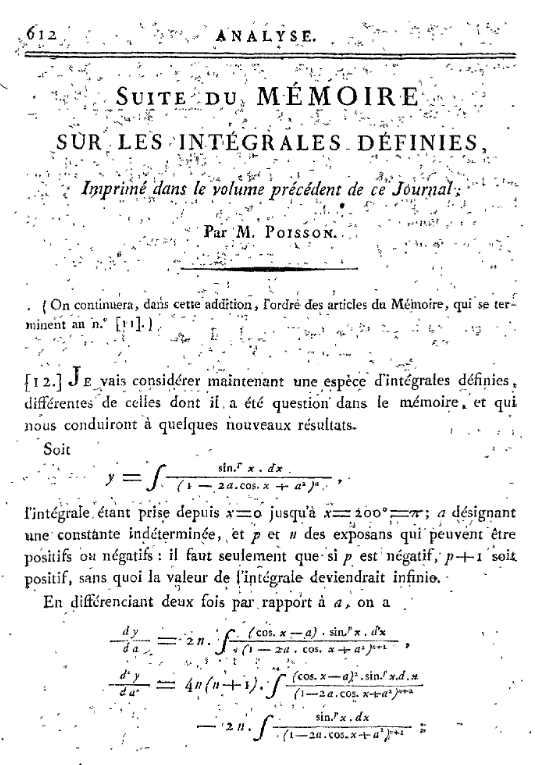
\includegraphics[scale=0.08]{illustrations/Journal_de_l_ecole_polytechnique_cahier_17_1815.png}
    % 
\includepdf[pages={3},scale=.4]{Journal_de_l_ecole_polytechnique_cahier_17_1815.pdf}
    \caption{\chevron{Suite du mémoire sur les intégrales définies}, Journal de l'École polytechnique, Cahier 17, X (1815), 612-631 (\url{https://gallica.bnf.fr/ark:/12148/bpt6k433673r/f614.item})}
\end{marginfigure}


\begin{subappendices}
\section{Théorèmes utilisés}

\begin{theo}[Intégration par parties généralisée, Source : \cite{acamanes}]\label{theo:ippgeneralisees}
    Soient $f$ et $g$ deux fonctions de classe $\mathscr{C}^1$ sur $I$. Si la fonction $fg$ a une limite finie en $a$ et en $b$, alors les intégrales
    \[
    \int_a^b f'(t)g(t) \d t \text{ et } \int_a^b f(t) g'(t) \d t
    \]
    sont de même nature. Si ces quantités sont convergentes, en notant
    \[
        [f(t)g(t)]_a^b = \lim_{x \to b^-} \big(f(x)g(x)\big) - \lim_{x \to a^+} \big(f(x)g(x)\big),
    \]
    on obtient la relation
    \[
    \int_a^b f'(t) g(t) \d t = \left[f(t)g(t)\right]_a^b - \int_a^b f(t) g'(t) \d t.
    \]
\end{theo}


\setchapterstyle{plain} % Output plain chapters from this point onwards

% \begin{subappendices}
\section{Diagrammes de décision}

% Diagrammes de decision
\subsection{Calculs d'intégrales}
%========
\chapter{Calculs d'intégrales}

\bigskip

\begin{center}
\begin{tikzpicture}[scale=0.75, every node/.style={transform shape}]
  % Place nodes
  \node [block] (init) {$\int_a^b f(t) \d t =~?$};
  %% Dérivées usuelles
  \node [decision, below=of init] (usuelle) {$f$ fonction usuelle};
  \node [cloud, right=of usuelle, yshift=1cm] (usuelle_oui) {$f(x) = c \rightsquigarrow \int_a^b f(t) \d t = \left[c t\right]_{a}^{b}$\\
  $f(x) = x^\alpha \rightsquigarrow \int_a^b f(t) \d t = \left[\frac{t^{\alpha+1}}{\alpha+1}\right]_{a}^{b},\, \alpha \neq -1$\\
  $f(x) = \frac{1}{x} \rightsquigarrow \int_a^b f(t) \d t = \left[\ln(t)\right]_{a}^{b}$\\
  $f(x) = \e^{\alpha x} \rightsquigarrow \int_a^b f(t) \d t = \left[\frac{\e^{\alpha x}}{\alpha}\right]_{a}^{b},\, \alpha \neq 0$\\
  };
  %% linearite
  \node [decision, text width=10em, below=of usuelle] (linearite) {$f(x) = a u'(x) + b v'(x)$};
  \node [cloud, right=of linearite] (linearite_oui) {$\int_a^b f(t) \d t = \left[a u(t) + b v(t)\right]_{a}^{b}$};
  %% puissance
  \node [decision, text width=10em, below=of linearite] (puissance) {$f(x) = u'(x) u(x)^\alpha$};
  \node [cloud, right=of puissance] (puissance_oui) {$\int_a^b f(t) \d t = \left[\frac{u(t)^{\alpha+1}}{\alpha+1}\right]_{a}^{b},\, \alpha \neq -1$};
  %% logarithme
  \node [decision, text width=10em, below=of puissance] (logarithme) {$f(x) = \frac{u'(x)}{u(x)}$};
  \node [cloud, right=of logarithme] (logarithme_oui) {$\int_a^b f(t) \d t = \left[\ln\abs{u(t)}\right]_{a}^{b}$};
  %% exponentielle
  \node [decision, text width=10em, below=of logarithme] (exponentielle) {$f(x) = u'(x) \e^{u(x)}$};
  \node [cloud, right=of exponentielle] (exponentielle_oui) {$\int_a^b f(t) \d t = \left[\e^{u(t)}\right]_{a}^{b}$};
  %% produit
  \node [decision, text width=10em, below=of exponentielle] (produit) {$f(x) = u'(x) \times v(x)$};
  \node [cloud, right=of produit] (produit_oui) {Intégration par parties\\
  $u$ et $v$ dérivables et de dérivées continues sur $[a, b]$\\
  $\int_a^b f(t) \d t = \left[u(t) v(t)\right]_{a}^{b} - \int_a^b u(t) v'(t) \d t$\\
  };

  
  % Draw edges
  \path [line] (init) --
      node [color=black, sloped, above] {}
      (usuelle);
  % usuelle
  \path [line] (usuelle) --
      node [color=black, sloped, above] {oui}
      (usuelle_oui);
  \path [line] (usuelle) --
      node [color=black, sloped, above] {non}
      (linearite);
  % linearite
  \path [line] (linearite) --
      node [color=black, sloped, above] {oui}
      (linearite_oui);
  \path [line] (linearite) --
      node [color=black, sloped, above] {non}
      (puissance);
  % \path [draw, very thick, color=black] (linearite_oui.east) --
      % ($(produit_oui.east) + (4,0)$);
  % % produit
  % \path [line] (produit) --
      % node [color=black, sloped, above] {oui}
      % (produit_oui);
  % \path [line] (produit) --
      % node [color=black, sloped, above] {non}
      % (quotient);
  % \path [draw, very thick, color=black] (produit_oui.east) --
      % ($(produit_oui.east) + (4,0)$);
  % % quotient
  % \path [line] (quotient) --
      % node [color=black, sloped, above] {oui}
      % (quotient_oui);
  % \path [line] (quotient) --
      % node [color=black, sloped, above] {non}
      % (puissance);
  % \path [draw, very thick, color=black] (quotient_oui.east) --
      % ($(produit_oui.east) + (4,0)$);
  % puissance
  \path [line] (puissance) --
      node [color=black, sloped, above] {oui}
      (puissance_oui);
  \path [line] (puissance) --
      node [color=black, sloped, above] {non}
      (logarithme);
  % \path [draw, very thick, color=black] (puissance_oui.east) --
      % ($(produit_oui.east) + (4,0)$);
  % logarithme
  \path [line] (logarithme) --
      node [color=black, sloped, above] {oui}
      (logarithme_oui);
  \path [line] (logarithme) --
      node [color=black, sloped, above] {non}
      (exponentielle);
  % \path [draw, very thick, color=black] (logarithme_oui.east) --
      % ($(produit_oui.east) + (4,0)$);
  % exponentielle
  \path [line] (exponentielle) --
      node [color=black, sloped, above] {oui}
      (exponentielle_oui);
  \path [line] (exponentielle) --
      node [color=black, sloped, above] {non}
      (produit);
  % \path [line] (exponentielle_oui.east) --
      % ($(produit_oui.east) + (4,0)$)
      % -- ($(init.east) + (13, 0)$) --
      % node [color=black, sloped, above] {Calcul de $u',\, v'$}
      % (init.east);
  % produit
  \path [line] (produit) --
      node [color=black, sloped, above] {oui}
      (produit_oui);
  \path [line] (produit_oui.east) --
      ($(produit_oui.east) + (3,0)$)
      to[bend right=50]
      ($(init.east) + (12,0)$) --
      node [color=black, sloped, above] {Calcul de la nouvelle intégrale} 
      (init.east);
      \end{tikzpicture}
      \end{center}
\subsection{Intégrales généralisées}
\todoarmand{Reprendre l'espacement entre les blocs}
\begin{center}
\begin{tikzpicture}[scale=1, every node/.style={transform shape}]

  \node [block] (init) {$\displaystyle\int_I f$ ?};
  \node [decision, below =of init] (regularite) {Régularité ?};
  \node [decision, right =of regularite] (decoupage) {$\interoo{a}{b}$\\$=$\\$\interof{a}{c} \cup \interfo{c}{b}$};
  \node [decision, below =of regularite] (reel) {$a \in \R$};
  \node [decision, right =of reel] (plg) {Prolongement \\ continu};
  \node [cloud, right =of plg] (cv) {Converge};
  \node [decision, below =of reel] (primitive) {$\displaystyle\int^x f = F(x)$};
  \node [decision, right =of primitive] (limfct) {$F(a) \to \ell \in \mathbb{R}$};
  \node [decision, below =of primitive] (positive) {$f \geqslant 0$};
  \node [decision, right =of positive] (comparaison) {$f = O_a(g)$};
  \node [cloud, above right =of comparaison, yshift=-1.7cm] (dv) {diverge${}^\ast$};
  \node [decision, left =of positive] (integrable) {$\displaystyle\int_I |f|$};
  \node [decision, below =of positive] (chgtvar) {Changement \\ de variables};
  \node [block, right =of chgtvar] (chgtvarint) {$\displaystyle\int_J |\varphi'|  \cdot f \circ \varphi$\\ converge ?};
  \node [decision, below =of chgtvar] (ipp) {\textsc{i.p.p.}};
  \node [block, right =of ipp] (ippint) {$\displaystyle\int_I u' v$\\ converge ?};
  \node [cloud, left =of ipp, xshift=2cm] (etc) {Autres idées ?};

  % Draw edges
  \path [line] (init) -- (regularite);
  \path [line] ($(regularite)!0.5!(reel)$) coordinate (rrm)
      (regularite) -- node [above] {\contour{white}{$1$ pt}}
                      node [below] {\contour{white}{$\interof{a}{c}$, $\interfo{c}{a}$}}
      (reel);
  \path [line] (regularite) -- node [above] {plusieurs} node [below] {pts} (decoupage);
  \path [draw, very thick] (decoupage) |- (rrm);
  \path [line] (reel) -- node [midway] {\contour{white}{oui}} (plg);
  \path [line] (plg) -- node [midway] {\contour{white}{oui}} (cv);
  \path [line] ($(reel)!0.5!(primitive)$) coordinate (rpm)
    (reel) -- node [near start, sloped, above] {non} (primitive);
  \path [draw, very thick] (plg) |- node [near start, sloped, above] {non} (rpm);
  \path [line] (primitive) -- node [midway] {\contour{white}{oui}} (limfct);
  \path [line] ($(primitive)!0.5!(positive)$) coordinate (ppm)
    (primitive) -- node [near start, sloped, below] {non} (positive);
  \path [line] ([yshift=5pt]limfct.east) -| node [near start, above] {$\ell\in\R$} (cv);
  \path [line] ([yshift=-5pt] limfct.east) -| node [near end, yshift=3pt] {\contour{white}{$\ell\in \{-\infty, +\infty\}$}} (dv);
  \path [draw, very thick] (limfct) |- node [near start, sloped, above] {non} (ppm);
  \path [line] ([yshift=5pt] positive.west) -- node [above] {non (1)} ([yshift=5pt] integrable.east);
  \path [line] ([yshift=-5pt] integrable.east) -- ([yshift=-5pt] positive.west);
  \path [line] (positive) -- (comparaison);
  \path [line] ([yshift=5pt] comparaison.east) -| node [near end, yshift=-5pt] {\contour{white}{$f \sim_a g$ et $\displaystyle\int_I |g|$ diverge}} % node [near start, below] {$\displaystyle\int_I |g|$ diverge} 
  (dv);
  \path [line] ([yshift=-5pt] comparaison.east) -| node [below, sloped, near end] {$\int_I |g|$ converge} (cv);
  \path [line] ($(positive)!0.5!(chgtvar)$) coordinate (pcm)
      (positive) -- node [sloped, below] {non (2)} (chgtvar);


  \path [draw, very thick] (comparaison.south) |- (pcm);
  \path [line] (chgtvar) -- node [midway] {\contour{white}{$\mathscr{C}^1$ bijectif}} (chgtvarint);
  \path [line] (chgtvarint.south west) -- node [midway, sloped] {\contour{white}{non}} (ipp.north east);
  \path [line] (ipp) -- node [above] {crochet} node [below] {converge} (ippint);
  \path [line] (ippint.east) -- ([xshift=5.7cm]ippint.east) |- (init.east);
  \path [line] (ipp.west) -- (etc.east);
  \path [line] (chgtvarint.east) -- ([xshift=5cm]chgtvarint.east) |- (init.east);\node [block] (init) {$\displaystyle\int_I f$ ?};
  \node [decision, below =of init] (regularite) {Régularité ?};

\end{tikzpicture}
\end{center}
%
$\ast$ Si $g = o_a(f)$ sont positives et $\int_a g$ diverge, alors $\int_a f$ diverge.

\end{subappendices}

 %\end{subappendices}

\setchapterstyle{kao} % Choose the default chapter heading style


% Diagrammes de decision
% %========
\chapter{Calculs d'intégrales}

\bigskip

\begin{center}
\begin{tikzpicture}[scale=0.75, every node/.style={transform shape}]
  % Place nodes
  \node [block] (init) {$\int_a^b f(t) \d t =~?$};
  %% Dérivées usuelles
  \node [decision, below=of init] (usuelle) {$f$ fonction usuelle};
  \node [cloud, right=of usuelle, yshift=1cm] (usuelle_oui) {$f(x) = c \rightsquigarrow \int_a^b f(t) \d t = \left[c t\right]_{a}^{b}$\\
  $f(x) = x^\alpha \rightsquigarrow \int_a^b f(t) \d t = \left[\frac{t^{\alpha+1}}{\alpha+1}\right]_{a}^{b},\, \alpha \neq -1$\\
  $f(x) = \frac{1}{x} \rightsquigarrow \int_a^b f(t) \d t = \left[\ln(t)\right]_{a}^{b}$\\
  $f(x) = \e^{\alpha x} \rightsquigarrow \int_a^b f(t) \d t = \left[\frac{\e^{\alpha x}}{\alpha}\right]_{a}^{b},\, \alpha \neq 0$\\
  };
  %% linearite
  \node [decision, text width=10em, below=of usuelle] (linearite) {$f(x) = a u'(x) + b v'(x)$};
  \node [cloud, right=of linearite] (linearite_oui) {$\int_a^b f(t) \d t = \left[a u(t) + b v(t)\right]_{a}^{b}$};
  %% puissance
  \node [decision, text width=10em, below=of linearite] (puissance) {$f(x) = u'(x) u(x)^\alpha$};
  \node [cloud, right=of puissance] (puissance_oui) {$\int_a^b f(t) \d t = \left[\frac{u(t)^{\alpha+1}}{\alpha+1}\right]_{a}^{b},\, \alpha \neq -1$};
  %% logarithme
  \node [decision, text width=10em, below=of puissance] (logarithme) {$f(x) = \frac{u'(x)}{u(x)}$};
  \node [cloud, right=of logarithme] (logarithme_oui) {$\int_a^b f(t) \d t = \left[\ln\abs{u(t)}\right]_{a}^{b}$};
  %% exponentielle
  \node [decision, text width=10em, below=of logarithme] (exponentielle) {$f(x) = u'(x) \e^{u(x)}$};
  \node [cloud, right=of exponentielle] (exponentielle_oui) {$\int_a^b f(t) \d t = \left[\e^{u(t)}\right]_{a}^{b}$};
  %% produit
  \node [decision, text width=10em, below=of exponentielle] (produit) {$f(x) = u'(x) \times v(x)$};
  \node [cloud, right=of produit] (produit_oui) {Intégration par parties\\
  $u$ et $v$ dérivables et de dérivées continues sur $[a, b]$\\
  $\int_a^b f(t) \d t = \left[u(t) v(t)\right]_{a}^{b} - \int_a^b u(t) v'(t) \d t$\\
  };

  
  % Draw edges
  \path [line] (init) --
      node [color=black, sloped, above] {}
      (usuelle);
  % usuelle
  \path [line] (usuelle) --
      node [color=black, sloped, above] {oui}
      (usuelle_oui);
  \path [line] (usuelle) --
      node [color=black, sloped, above] {non}
      (linearite);
  % linearite
  \path [line] (linearite) --
      node [color=black, sloped, above] {oui}
      (linearite_oui);
  \path [line] (linearite) --
      node [color=black, sloped, above] {non}
      (puissance);
  % \path [draw, very thick, color=black] (linearite_oui.east) --
      % ($(produit_oui.east) + (4,0)$);
  % % produit
  % \path [line] (produit) --
      % node [color=black, sloped, above] {oui}
      % (produit_oui);
  % \path [line] (produit) --
      % node [color=black, sloped, above] {non}
      % (quotient);
  % \path [draw, very thick, color=black] (produit_oui.east) --
      % ($(produit_oui.east) + (4,0)$);
  % % quotient
  % \path [line] (quotient) --
      % node [color=black, sloped, above] {oui}
      % (quotient_oui);
  % \path [line] (quotient) --
      % node [color=black, sloped, above] {non}
      % (puissance);
  % \path [draw, very thick, color=black] (quotient_oui.east) --
      % ($(produit_oui.east) + (4,0)$);
  % puissance
  \path [line] (puissance) --
      node [color=black, sloped, above] {oui}
      (puissance_oui);
  \path [line] (puissance) --
      node [color=black, sloped, above] {non}
      (logarithme);
  % \path [draw, very thick, color=black] (puissance_oui.east) --
      % ($(produit_oui.east) + (4,0)$);
  % logarithme
  \path [line] (logarithme) --
      node [color=black, sloped, above] {oui}
      (logarithme_oui);
  \path [line] (logarithme) --
      node [color=black, sloped, above] {non}
      (exponentielle);
  % \path [draw, very thick, color=black] (logarithme_oui.east) --
      % ($(produit_oui.east) + (4,0)$);
  % exponentielle
  \path [line] (exponentielle) --
      node [color=black, sloped, above] {oui}
      (exponentielle_oui);
  \path [line] (exponentielle) --
      node [color=black, sloped, above] {non}
      (produit);
  % \path [line] (exponentielle_oui.east) --
      % ($(produit_oui.east) + (4,0)$)
      % -- ($(init.east) + (13, 0)$) --
      % node [color=black, sloped, above] {Calcul de $u',\, v'$}
      % (init.east);
  % produit
  \path [line] (produit) --
      node [color=black, sloped, above] {oui}
      (produit_oui);
  \path [line] (produit_oui.east) --
      ($(produit_oui.east) + (3,0)$)
      to[bend right=50]
      ($(init.east) + (12,0)$) --
      node [color=black, sloped, above] {Calcul de la nouvelle intégrale} 
      (init.east);
      \end{tikzpicture}
      \end{center}
% \begin{center}
\begin{tikzpicture}[scale=1, every node/.style={transform shape}]

  \node [block] (init) {$\displaystyle\int_I f$ ?};
  \node [decision, below =of init] (regularite) {Régularité ?};
  \node [decision, right =of regularite] (decoupage) {$\interoo{a}{b}$\\$=$\\$\interof{a}{c} \cup \interfo{c}{b}$};
  \node [decision, below =of regularite] (reel) {$a \in \R$};
  \node [decision, right =of reel] (plg) {Prolongement \\ continu};
  \node [cloud, right =of plg] (cv) {Converge};
  \node [decision, below =of reel] (primitive) {$\displaystyle\int^x f = F(x)$};
  \node [decision, right =of primitive] (limfct) {$F(a) \to \ell \in \mathbb{R}$};
  \node [decision, below =of primitive] (positive) {$f \geqslant 0$};
  \node [decision, right =of positive] (comparaison) {$f = O_a(g)$};
  \node [cloud, above right =of comparaison, yshift=-1.7cm] (dv) {diverge${}^\ast$};
  \node [decision, left =of positive] (integrable) {$\displaystyle\int_I |f|$};
  \node [decision, below =of positive] (chgtvar) {Changement \\ de variables};
  \node [block, right =of chgtvar] (chgtvarint) {$\displaystyle\int_J |\varphi'|  \cdot f \circ \varphi$\\ converge ?};
  \node [decision, below =of chgtvar] (ipp) {\textsc{i.p.p.}};
  \node [block, right =of ipp] (ippint) {$\displaystyle\int_I u' v$\\ converge ?};
  \node [cloud, left =of ipp, xshift=2cm] (etc) {Autres idées ?};

  % Draw edges
  \path [line] (init) -- (regularite);
  \path [line] ($(regularite)!0.5!(reel)$) coordinate (rrm)
      (regularite) -- node [above] {\contour{white}{$1$ pt}}
                      node [below] {\contour{white}{$\interof{a}{c}$, $\interfo{c}{a}$}}
      (reel);
  \path [line] (regularite) -- node [above] {plusieurs} node [below] {pts} (decoupage);
  \path [draw, very thick] (decoupage) |- (rrm);
  \path [line] (reel) -- node [midway] {\contour{white}{oui}} (plg);
  \path [line] (plg) -- node [midway] {\contour{white}{oui}} (cv);
  \path [line] ($(reel)!0.5!(primitive)$) coordinate (rpm)
    (reel) -- node [near start, sloped, above] {non} (primitive);
  \path [draw, very thick] (plg) |- node [near start, sloped, above] {non} (rpm);
  \path [line] (primitive) -- node [midway] {\contour{white}{oui}} (limfct);
  \path [line] ($(primitive)!0.5!(positive)$) coordinate (ppm)
    (primitive) -- node [near start, sloped, below] {non} (positive);
  \path [line] ([yshift=5pt]limfct.east) -| node [near start, above] {$\ell\in\R$} (cv);
  \path [line] ([yshift=-5pt] limfct.east) -| node [near end, yshift=3pt] {\contour{white}{$\ell\in \{-\infty, +\infty\}$}} (dv);
  \path [draw, very thick] (limfct) |- node [near start, sloped, above] {non} (ppm);
  \path [line] ([yshift=5pt] positive.west) -- node [above] {non (1)} ([yshift=5pt] integrable.east);
  \path [line] ([yshift=-5pt] integrable.east) -- ([yshift=-5pt] positive.west);
  \path [line] (positive) -- (comparaison);
  \path [line] ([yshift=5pt] comparaison.east) -| node [near end, yshift=-5pt] {\contour{white}{$f \sim_a g$ et $\displaystyle\int_I |g|$ diverge}} % node [near start, below] {$\displaystyle\int_I |g|$ diverge} 
  (dv);
  \path [line] ([yshift=-5pt] comparaison.east) -| node [below, sloped, near end] {$\int_I |g|$ converge} (cv);
  \path [line] ($(positive)!0.5!(chgtvar)$) coordinate (pcm)
      (positive) -- node [sloped, below] {non (2)} (chgtvar);


  \path [draw, very thick] (comparaison.south) |- (pcm);
  \path [line] (chgtvar) -- node [midway] {\contour{white}{$\mathscr{C}^1$ bijectif}} (chgtvarint);
  \path [line] (chgtvarint.south west) -- node [midway, sloped] {\contour{white}{non}} (ipp.north east);
  \path [line] (ipp) -- node [above] {crochet} node [below] {converge} (ippint);
  \path [line] (ippint.east) -- ([xshift=5.7cm]ippint.east) |- (init.east);
  \path [line] (ipp.west) -- (etc.east);
  \path [line] (chgtvarint.east) -- ([xshift=5cm]chgtvarint.east) |- (init.east);\node [block] (init) {$\displaystyle\int_I f$ ?};
  \node [decision, below =of init] (regularite) {Régularité ?};

\end{tikzpicture}
\end{center}
%
$\ast$ Si $g = o_a(f)$ sont positives et $\int_a g$ diverge, alors $\int_a f$ diverge.


% \printbibliography[heading=bibintoc, title=Références]

% % \printindex % Output the index

\end{document}
